\documentclass[11pt,titlepage,a4paper,oneside]{book}

%% --- Encodage et langue ---
\usepackage[T1]{fontenc}
\usepackage[utf8]{inputenc}
\usepackage{lmodern}
\usepackage[french]{babel}
\usepackage[babel=true]{csquotes}

%% --- Mise en page ---
\usepackage[a4paper, top=25mm, bottom=25mm, left=35mm, right=25mm]{geometry}
\usepackage{setspace}
\onehalfspacing
\usepackage{microtype}
\emergencystretch=2em

%% --- Mathématiques ---
\usepackage{amsmath}
\usepackage{amssymb}
\usepackage{latexsym}
\everymath{\displaystyle}

%% --- Graphiques ---
\usepackage{graphicx}
\usepackage{overpic}
\usepackage{color}
\usepackage{xcolor}
\usepackage{epsfig}
\graphicspath{{figures/}}

%% --- Tableaux ---
\usepackage{booktabs}
\usepackage{multirow}
\usepackage{tabularx}
\usepackage[table]{xcolor}
\usepackage{float}
\usepackage{lscape}
\usepackage{rotate}
\setlength\belowcaptionskip{0.25cm}

\usepackage{tikz}
\usetikzlibrary{calc,positioning,shapes.geometric}

%% --- Texte ---
\usepackage{fancybox}
\usepackage{tcolorbox}
\usepackage{verbatim}
\usepackage{enumitem}
\usepackage{calc}

%% --- Headers ---
\usepackage{mychapter,mymacros}
\input{PhS_Header}

%% --- TOC ---
\usepackage{minitoc}
\dominitoc
\setcounter{minitocdepth}{2}

%% --- Algo ---
\usepackage{algorithm}
\usepackage{algorithmicx}
\usepackage{algpseudocode}

%% --- Bibliographie ---
\usepackage[backend=biber, style=numeric]{biblatex}
\addbibresource{Thesis-report.bib}
\addbibresource{webographie.bib}

%% --- PDF ---
\usepackage{makeidx}
\usepackage{hyperref}
\usepackage{pdfpages}

%% --- IMPORTANT (corrigé) ---
\usepackage{tikz}
\usepackage{fontawesome5}

%% --- Couleurs ---
\definecolor{grisclair}{gray}{0.2}
\definecolor{light-gary}{gray}{0.95}
\definecolor{lgray}{gray}{0.85}
\definecolor{gris}{gray}{0.45}

%% --- Environnements ---
\newtheorem{exmp}{Example}[section]
\newenvironment{remarque}{\textbf{Remarque :}}{}
\newlength{\longueurequation}
\newlength{\longueurrestante}

\newcommand{\me}[1]{%
  \longueurrestante=\linegoal%
  \settowidth{\longueurequation}{$#1$}%
  \ifthenelse{\longueurequation>\longueurrestante}%
    {\begin{displaymath}#1\end{displaymath}}{$#1$}%
}

%%%%%%%%%%%%%%%%%%%%%%%%%%%%%%%%%%%%%%%%%%%%%%%%%%%%%%%%%%%%%%%%%%%%%%
\begin{document}

\includepdf{Chapitres/Page_garde_BC.pdf}
\thispagestyle{empty}

%%%%%%%%%%%%%%%%%%%%%%%%%%%%%%%%%%%%%%%%%%%%%%%%%%%%%%%%%%%%%%%%%%%%%%%%%%%
\chapter*{Déclaration sur l'utilisation de l'Intelligence Artificielle Générative}
%%%%%%%%%%%%%%%%%%%%%%%%%%%%%%%%%%%%%%%%%%%%%%%%%%%%%%%%%%%%%%%%%%%%%%%%%%%
Nous déclarons par la présente avoir utilisé des outils d'intelligence artificielle générative (IAG) comme suit :
\begin{enumerate}
    \item \textbf{Reformulation} : Nous avons utilisé ........ pour reformuler et affiner notre texte, en garantissant sa clarté et son originalité. Nous avons systématiquement vérifié et parfois modifié les résultats de l'IAG.
    \item \textbf{Débogage de code} : Nous avons utilisé ..... comme assistant de développement pour identifier les erreurs potentielles, optimiser la structure du code et suggérer des améliorations algorithmiques. Chaque suggestion a été soigneusement évaluée et adaptée à nos besoins spécifiques.
\end{enumerate}

\par Ces outils d'IAG ont été utilisés comme technologies de support pour améliorer notre rapport, les processus fondamentaux de recherche, de rédaction et de résolution de problèmes demeurant les nôtres.

\begin{tcolorbox}[title=\textbf{Attention},    
colback=yellow!10,
    colframe=red!75!black,
    colbacktitle=red!85!black,
    coltitle=white,
    fonttitle=\large\bfseries,
    boxrule=0.5mm]
Vous devez déclarer toutes les intelligences artificielles génératives utilisées, tant pour la rédaction du rapport que pour la réalisation de l'application. Cette déclaration doit être exhaustive et inclure :
\begin{itemize}
   \item Les outils d'IA utilisés pour la génération de texte
   \item Les assistants IA utilisés pour la génération ou la révision de code
   \item Les modèles d'IA utilisés pour la création de visuels ou de maquettes
   \item Toute autre utilisation d'IA générative dans le cadre de ce projet
\end{itemize}
Cette déclaration doit apparaître dans une section dédiée de votre rapport.
\end{tcolorbox}
\thispagestyle{empty}
\strut
\thispagestyle{empty}

\include{Chapitres/dedication}
\thispagestyle{empty}

%%%%%%%%%%%%%%%%%%%%%%%%%%%%%%%%%%%%%%%%%%%%%%%%%%%%%%%%%%%%%%%%%%%%%%%%%%%
\chapter*{Remerciements}
\label{sec:Acknowledgements}
\thispagestyle{empty}
%%%%%%%%%%%%%%%%%%%%%%%%%%%%%%%%%%%%%%%%%%%%%%%%%%%%%%%%%%%%%%%%%%%%%%%%%%%
Je tiens tout d'abord à exprimer ma profonde gratitude à ...


\thispagestyle{empty}

%%%%%%%%%%%%%%%%%%%%%%%%%%%%%%%%%%%%%%%%%%%%%%%%%%%%%%%%%%%%%%%%%%%%%%%%%%%
\newpage
\begin{center}
\textbf{Abstract}
\end{center}
%%%%%%%%%%%%%%%%%%%%%%%%%%%%%%%%%%%%%%%%%%%%%%%%%%%%%%%%%%%%%%%%%%%%%%%%%%%

Un résumé de votre PFE en Anglais

%%%%%%%%%%%%%%%%%%%%%%%%%%%%%%%%%%%%%%%%%%%%%%%%%%%%%%%%%%%%%%%%%%%%%%%%%%%
\begin{center}
\textbf{Résumé}
\end{center}
%%%%%%%%%%%%%%%%%%%%%%%%%%%%%%%%%%%%%%%%%%%%%%%%%%%%%%%%%%%%%%%%%%%%%%%%%%%

Un résumé de votre PFE en Français

\thispagestyle{empty}
\strut
\begin{tcolorbox}[
   title=Important,
   colback=blue!5,
   colframe=blue!75,
   coltitle=white,
   fonttitle=\bfseries
]
Cette page contenant l'abstract et le résumé doit être imprimée au verso du rapport, sur la face opposée à la page de garde.
\medskip
\textbf{Note :} Assurez-vous que cette page soit correctement positionnée lors de l'impression du document final.
\end{tcolorbox}

\pagestyle{headings}

\pagenumbering{roman}
\tableofcontents
\listoftables
\thispagestyle{empty}
\listoffigures
\thispagestyle{empty}

\include{Chapitres/Notations}

\pagenumbering{arabic}

\chapter*{Introduction}
\addstarredchapter{Introduction}
%%%%%%%%%%%%%%%%%%%%%%%%%%%%%%%%%%%%%%%%%%%%%%%%%%%%%%%%%%%%%%%%%%%%%%%%

L'introduction précède le corps du mémoire. Cette partie essentielle permet
d'introduire le lecteur au sujet traité et de présenter les enjeux principaux.
Le texte se doit d'être accrocheur afin de susciter l'intérêt du lecteur pour
la suite. C'est un travail rédactionnel qui nécessite une attention particulière
pour produire un mémoire original et démontrer son implication dans la recherche.

Le mémoire est organisé comme suit :
Le premier chapitre présente le projet décisionnel dans son contexte général.
Le deuxième chapitre identifie les besoins d'affaires et expose l'architecture technique retenue.
Le troisième chapitre traite de la modélisation conceptuelle et physique de l'entrepôt de données.
Le quatrième chapitre détaille le processus d'intégration des données.
Le cinquième chapitre présente la conception, le développement et le déploiement de la plateforme décisionnelle.

\begin{tcolorbox}[
    enhanced,
    title={\textbf{Attention : Règles de ponctuation en français}},
    colback=yellow!10,
    colframe=red!75!black,
    colbacktitle=red!85!black,
    coltitle=white,
    fonttitle=\large\bfseries,
    boxrule=0.5mm
]

\textbf{Règles de ponctuation française :}

\begin{itemize}[leftmargin=*]
    \item Le point (.) : 
        \begin{itemize}
            \item Pas d'espace avant
            \item Un espace après
            \item Suivi d'une majuscule pour nouvelle phrase
        \end{itemize}
    
    \item La virgule (,) :
        \begin{itemize}
            \item Pas d'espace avant
            \item Un espace après
            \item Sépare les éléments d'une énumération ou les propositions
        \end{itemize}
    
    \item Le point-virgule (;) :
        \begin{itemize}
            \item Une espace fine avant avec \verb|~|
            \item Un espace après
            \item Sépare deux propositions liées par le sens
        \end{itemize}
    
    \item Les deux-points (:) :
        \begin{itemize}
            \item Une espace fine avant avec \verb|~|
            \item Un espace après
            \item Introduisent une énumération, une citation ou une explication
        \end{itemize}
    
    \item Les points de suspension (...) :
        \begin{itemize}
            \item Pas d'espace avant
            \item Un espace après
            \item Exactement trois points
        \end{itemize}
    
    \item Les points d'exclamation (!) et d'interrogation (?) :
        \begin{itemize}
            \item Une espace fine avant avec \verb|~|
            \item Un espace après
            \item Pas de point après ces signes
        \end{itemize}
    
    \item Les guillemets français (« ») :
        \begin{itemize}
            \item Une espace fine après l'ouverture
            \item Une espace fine avant la fermeture
            \item Utilisés pour les citations directes
        \end{itemize}
    
    \item Les parenthèses () et les crochets [] :
        \begin{itemize}
            \item Pas d'espace à l'intérieur
            \item Collés au mot qu'ils encadrent
            \item Un espace avant l'ouverture et après la fermeture
        \end{itemize}
\end{itemize}

\textbf{Note importante :} En typographie française, on distingue l'espace normal de l'espace fine. L'espace fine est utilisée avant les signes de ponctuation doubles (; : ! ? »), tandis que l'espace normal est utilisé après tous les signes de ponctuation.

\end{tcolorbox}


%%%%%%%%%%%%%%%%%%%%%%%%%%%%%%%%%%%%%%%%%%%%%%%%%%%%%%%%%%%%%%%%%%%%%%%%%%
\chapter{Titre du chapitre}
\label{Chapitre1}
\addtocontents{mtc}{\protect\renewcommand{\protect\insertminitoc}{}}
%%%%%%%%%%%%%%%%%%%%%%%%%%%%%%%%%%%%%%%%%%%%%%%%%%%%%%%%%%%%%%%%%%%%%%%%%%
\section{Introduction}
\label{sec:Introduction1}
%%%%%%%%%%%%%%%%%%%%%%%%%%%%%%%%%%%%%%%%%%%%%%%%%%%%%%%%%%%%%%%%%%%%%%
Ce premier chapitre .... 

Voilà un exemple de citation à partir de la webographie \cite{stackoverflow:latex} et un exemple de citation à partir de la bibliographe \cite{Severson2019}.

\begin{tcolorbox}[
   title=Important,
   colback=blue!5,
   colframe=blue!75,
   coltitle=white,
   fonttitle=\bfseries
]
L'introduction d'un chapitre doit suivre la structure suivante :

1. Introduction générale du contexte
   \begin{itemize}
      \item Présentation du domaine général
      \item Contextualisation du sujet
   \end{itemize}

2. Introduction spécifique du chapitre
   \begin{itemize}
      \item Présentation des concepts clés
      \item Énoncé de la problématique spécifique
   \end{itemize}

3. Plan du chapitre
   \begin{itemize}
      \item Présentation des différentes sections
      \item Annonce de la structure et de la progression logique
   \end{itemize}
   \textbf{Note:} Respectez cette stucture pour les introductions de tous vos chapitres.
\end{tcolorbox}

%%%%%%%%%%%%%%%%%%%%%%%%%%%%%%%%%%%%%%%%%%%%%%%%%%%%%%%%%%%%%%%%%%%%%%%%%%
\section{Présentation de l'établissement d'accueil}
\label{scetion1}
%%%%%%%%%%%%%%%%%%%%%%%%%%%%%%%%%%%%%%%%%%%%%%%%%%%%%%%%%%%%%%%%%%%%%%%%%%
Fournir une brève présentation de l'établissement d'accueil.

La Figure \ref{fig_ESEN} présente le logo de l'ESEN. Comme pour toute figure dans ce document, une description détaillée et une référence explicite sont nécessaires pour guider le lecteur dans sa compréhension.


\begin{figure}[H]
    \centering
    
\includegraphics[width=0.5\textwidth]{ESEN.png}
    \caption{Logo de l'ESEN}
    \label{fig_ESEN}
\end{figure}


%%%%%%%%%%%%%%%%%%%%%%%%%%%%%%%%%%%%%%%%%%%%%%%%%%%%%%%%%%%%%%%%%%%%%%%%%%
\section{Section 2}
%%%%%%%%%%%%%%%%%%%%%%%%%%%%%%%%%%%%%%%%%%%%%%%%%%%%%%%%%%%%%%%%%%%%%%%%%%
\textbf{Remarque:} Vous pouvez générer les tableaux avec \href{https://www.tablesgenerator.com/}{tablesgenerator.com}.

\begin{table}[H]
\centering
\caption{Titre du tableay}
\label{tab1}
\begin{tabular}{|p{3cm}|p{8cm}|}
\hline
\textbf{Colonne 1} & \textbf{Colonne 2} \\
\hline
Texte & Texte \\
\hline
\dots & \dots \\
\hline
\end{tabular}
\label{tab:ventes}
\end{table}
\begin{tcolorbox}[
   title=Important,
   colback=blue!5,
   colframe=blue!75,
   coltitle=white,
   fonttitle=\bfseries
]
Dans la rédaction de votre document, il est essentiel de respecter les conventions suivantes :
\begin{itemize}
   \item Chaque tableau et figure doit être décrit et référencé explicitement dans le texte
   \item Évitez les expressions imprécises comme ``ci-dessous'' ou ``ci-dessus''
   \item Utilisez toujours la commande \verb|\ref{}| pour faire référence aux éléments, par exemple :
   \begin{quote}
              \textit{``Comme le montre la Figure 1.1 (avec la commande \backslash ref\{\}),\hspace{0.2cm}les\hspace{0.2cm}résultats\hspace{0.2cm}indiquent...''}
       
       \textit{``Les données présentées dans le Tableau~i,j démontrent...''}
   \end{quote}

   \item Cette pratique permet une navigation plus claire et facilite la lecture du document
\end{itemize}
\end{tcolorbox}
%%%%%%%%%%%%%%%%%%%%%%%%%%%%%%%%%%%%%%%%%%%%%%%%%%%%%%%%%%%%%%%%%%%%%%%%%%
\subsection{Sous-section 1}
\dots
%%%%%%%%%%%%%%%%%%%%%%%%%%%%%%%%%%%%%%%%%%%%%%%%%%%%%%%%%%%%%%%%%%%%%%%%%%


%%%%%%%%%%%%%%%%%%%%%%%%%%%%%%%%%%%%%%%%%%%%%%%%%%%%%%%%%%%%%%%%%%%%%%%%%%
\subsection{Sous-section 2}
\dots
%%%%%%%%%%%%%%%%%%%%%%%%%%%%%%%%%%%%%%%%%%%%%%%%%%%%%%%%%%%%%%%%%%%%%%%%%%

%%%%%%%%%%%%%%%%%%%%%%%%%%%%%%%%%%%%%%%%%%%%%%%%%%%%%%%%%%%%%%%%%%%%%%%%%%
\section{Section 3}
\dots
%%%%%%%%%%%%%%%%%%%%%%%%%%%%%%%%%%%%%%%%%%%%%%%%%%%%%%%%%%%%%%%%%%%%%%%%%%

%%%%%%%%%%%%%%%%%%%%%%%%%%%%%%%%%%%%%%%%%%%%%%%%%%%%%%%%%%%%%%%%%%%%%%%%%%
\section{Conclusion}
%%%%%%%%%%%%%%%%%%%%%%%%%%%%%%%%%%%%%%%%%%%%%%%%%%%%%%%%%%%%%%%%%%%%%%%%%%
N'oubliez pas de conclure vos chapitres et de faire le lien avec le chapitre suivant.

%%%%%%%%%%%%%%%%%%%%%%%%%%%%%%%%%%%%%%%%%%%%%%%%%%%%%%%%%%%%%%%%%%%%%%%%%%%
\chapter{Étude de marché}
\label{Chapitre_2}
%%%%%%%%%%%%%%%%%%%%%%%%%%%%%%%%%%%%%%%%%%%%%%%%%%%%%%%%%%%%%%%%%%%%%%%%%%%

\textit{Ce chapitre ne se contente pas de décrire un marché~: il démontre l'existence d'une inefficience opérationnelle structurelle, non adressée, dont Vocallia constitue la réponse directe et défendable. L'analyse croise deux dynamiques complémentaires --- la réalité contrainte du commerce électronique tunisien et la maturité accélérée de l'IA vocale mondiale --- pour établir que l'opportunité est réelle, temporellement bornée et accessible à un premier entrant bien positionné. La méthodologie est pluridisciplinaire~: analyse PESTEL, forces de Porter, cadre TAM/SAM/SOM, étude exploratoire terrain, benchmark concurrentiel et cartographie des parties prenantes. Chaque couche analytique converge vers une même conclusion~: Vocallia répond à un besoin non optionnel, sur un marché captif, dans un horizon d'exécution qui ne restera pas ouvert indéfiniment.}

%%%%%%%%%%%%%%%%%%%%%%%%%%%%%%%%%%%%%%%%%%%%%%%%%%%%%%%%%%%%%%%%%%%%%%%%%%%
\section{Analyse macro-environnementale --- Cadre PESTEL}
\label{section2.1}
%%%%%%%%%%%%%%%%%%%%%%%%%%%%%%%%%%%%%%%%%%%%%%%%%%%%%%%%%%%%%%%%%%%%%%%%%%%

L'analyse PESTEL révèle un alignement remarquable de signaux favorables à l'émergence de Vocallia. Chaque dimension examinée --- politique, économique, sociale, technologique, écologique et légale --- renforce la même conclusion~: les conditions de fond sont réunies et le moment d'entrée sur le marché est optimal.

%%%%%%%%%%%%%%%%%%%%%%%%%%%%%%%%%%%%%%%%%%%%%%%%%%%%%%%%%%%%%%%%%%%%%%%%%%%
\subsection{Environnement politique et légal}
\label{section2.1.1}
%%%%%%%%%%%%%%%%%%%%%%%%%%%%%%%%%%%%%%%%%%%%%%%%%%%%%%%%%%%%%%%%%%%%%%%%%%%

Le Startup Act (Loi n\degre{}2018-20) offre aux structures labellisées des avantages concrets et immédiatement mobilisables~: subventions mensuelles jusqu'à 5\,000~dinars, congé entrepreneurial, exonérations fiscales pluriannuelles et accès facilité à des comptes en devises technologiques. Ce dispositif réduit directement le coût d'amorçage et améliore la compétitivité tarifaire dès le lancement.

Sur le plan réglementaire, la loi n\degre{}2004-63 sur la protection des données personnelles encadre le traitement des enregistrements vocaux. Vocallia intègre cette contrainte dès la conception (\emph{compliance by design})~: consentement explicite en début d'appel, rétention des données limitée à 30~jours, démarche de validation auprès de l'INPDP prévue avant tout déploiement commercial. La loi n\degre{}2000-83 sur le commerce électronique renforce par ailleurs la légitimité des services B2B numériques.

Ce cadre réglementaire, loin de constituer un simple coût de gestion, fonctionne en réalité comme une barrière à l'entrée au bénéfice de Vocallia. Toute solution internationale souhaitant pénétrer le marché tunisien devra investir dans une mise en conformité locale spécifique, sans bénéficier du Startup Act ni de la crédibilité institutionnelle que Vocallia construit dès l'origine. La rigueur réglementaire adoptée \emph{ab initio} crée ainsi un avantage compétitif défendable vis-à-vis des acteurs globaux, tout en réduisant le risque juridique perçu par les marchands partenaires --- accélérant de facto l'adoption commerciale.

%%%%%%%%%%%%%%%%%%%%%%%%%%%%%%%%%%%%%%%%%%%%%%%%%%%%%%%%%%%%%%%%%%%%%%%%%%%
\subsection{Environnement économique}
\label{section2.1.2}
%%%%%%%%%%%%%%%%%%%%%%%%%%%%%%%%%%%%%%%%%%%%%%%%%%%%%%%%%%%%%%%%%%%%%%%%%%%

Le e-commerce tunisien affiche une dynamique de croissance soutenue et durable~: 1\,126 sites marchands actifs en 2024, un volume de transactions de 1\,241,2~millions de dinars (BCT, 2024), et une progression de 41,6~\% du chiffre d'affaires entre juin 2022 et juin 2023, à 538,8~millions de dinars. Cette croissance n'est pas cyclique~: elle traduit une adoption progressive et durable des comportements d'achat numériques.

Mais le fait économique le plus structurant pour Vocallia est celui-ci~: \textbf{84~\% des transactions e-commerce tunisiennes sont réglées en espèces à la livraison (\emph{cash on delivery}).} Cette réalité rend la confirmation téléphonique préalable à l'expédition quasi-systématique --- et non optionnelle. Chaque commande expédiée sans confirmation expose le marchand à un retour non anticipé~: frais de transport aller-retour, manutention, réemballage et immobilisation temporaire du stock. En ordre de grandeur, le coût unitaire d'un colis retourné se situe entre 4 et 8~DT selon la catégorie de produit et la zone géographique de livraison.

Pour un e-commerçant de petite taille traitant 10 à 15 commandes par jour --- profil représentatif de la majorité des marchands tunisiens --- avec un taux de retour de l'ordre de 20 à 30~\%, la perte mensuelle liée aux livraisons échouées peut être estimée entre \textbf{300 et 700~DT}. À cela s'ajoute le coût de la main-d'\oe uvre affectée aux appels de confirmation~: qu'il s'agisse du gérant lui-même ou d'un employé dédié, ce poste représente entre 400 et 700~DT par mois --- pour une tâche répétitive, chronophage et parfaitement automatisable. Ces estimations restent des ordres de grandeur prudents~; elles suffisent néanmoins à établir que le problème n'est pas marginal~: même dans l'hypothèse basse, le coût cumulé des retours et de la gestion manuelle représente une charge mensuelle de 700 à 1\,400~DT --- significative pour une PME dont les marges opérationnelles sont étroites, et suffisante pour justifier économiquement le recours à une solution d'automatisation.

Le constat est arithmétique~: à mesure que le volume de commandes croît, la confirmation manuelle devient non scalable --- chaque palier de croissance impose un recrutement supplémentaire que les marges du secteur ne peuvent absorber. L'automatisation n'est plus une option d'optimisation~: elle devient une condition de survie opérationnelle.

\begin{figure}[H]
    \centering
    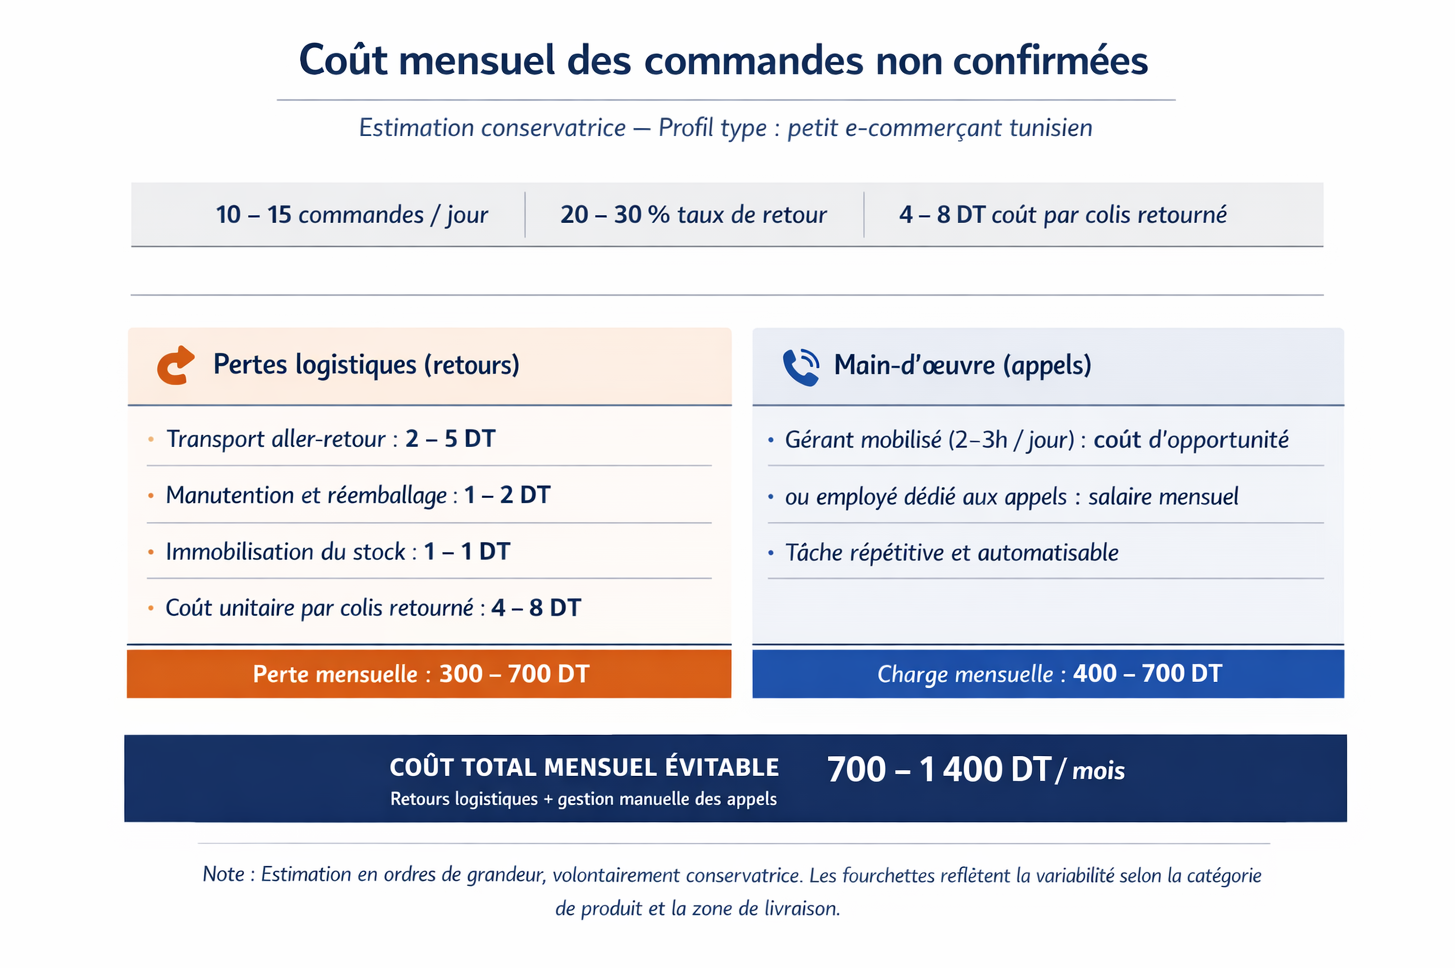
\includegraphics[width=0.92\textwidth]{figures/cout-commande-non-confirmee.png}
    \caption{Estimation du coût mensuel des commandes non confirmées --- Profil type d'un petit e-commerçant tunisien}
    \label{fig:cout-commande-non-confirmee}
\end{figure}

Le \emph{cash on delivery} n'est pas une anomalie appelée à disparaître~: il est ancré dans la méfiance du consommateur tunisien envers le paiement en ligne et dans l'absence d'infrastructure de confiance numérique généralisée. Tant que cette réalité persiste --- horizon incertain à moyen terme --- la confirmation téléphonique reste obligatoire, et donc automatisable. Plus décisif encore~: la croissance de 41,6~\% du secteur amplifie mécaniquement ce besoin, puisque chaque nouvelle commande génère un appel de confirmation supplémentaire. Le marché adressable de Vocallia croît ainsi sans effort commercial additionnel.

\textit{Source~: BCT, Bulletin sur les paiements en chiffres en Tunisie, exercice 2024 (mars 2025)~; BCT, Rapport sur les paiements 2022-2023~; estimation Vocallia sur la base des variables terrain, 2025.}

%%%%%%%%%%%%%%%%%%%%%%%%%%%%%%%%%%%%%%%%%%%%%%%%%%%%%%%%%%%%%%%%%%%%%%%%%%%
\subsection{Environnement social et démographique}
\label{section2.1.3}
%%%%%%%%%%%%%%%%%%%%%%%%%%%%%%%%%%%%%%%%%%%%%%%%%%%%%%%%%%%%%%%%%%%%%%%%%%%

La Tunisie compte 12,3~millions d'habitants en 2024, avec un taux de pénétration d'Internet de 66~\% (INS, 2022). Selon le baromètre MDWEB (vague~4, 2023), 75~\% des internautes ont déjà acheté en ligne, dont plus de la moitié au moins une fois par mois. Cette base d'acheteurs croissante alimente mécaniquement le volume de commandes des marchands, et donc le nombre d'appels de confirmation à passer. Il existe un seuil --- généralement situé autour de 50 à 80 commandes quotidiennes --- au-delà duquel la gestion manuelle des appels cesse d'être un choix organisationnel et devient un goulet d'étranglement~: le marchand ne peut plus croître sans automatiser ou recruter, et les marges du secteur interdisent le second. Le taux de chômage de 16,4~\% (INS, 2024), combiné à une pression à la hausse sur les coûts salariaux, renforce l'attractivité économique de l'automatisation pour des PME dont les marges opérationnelles restent étroites.

La dynamique d'ensemble est celle d'un cercle vicieux, représenté en figure~\ref{fig:cercle-vicieux}~: la croissance du marché génère davantage de commandes, donc davantage d'appels, ce qui sature le gérant, provoque des livraisons échouées, érode les marges et empêche le recrutement --- ramenant le marchand au point de départ. Chaque heure passée au téléphone à confirmer des commandes est une heure non investie dans la croissance --- et dans un marché en expansion de 41,6~\% par an, le coût de cette inaction se compose trimestre après trimestre.

\begin{figure}[H]
    \centering
    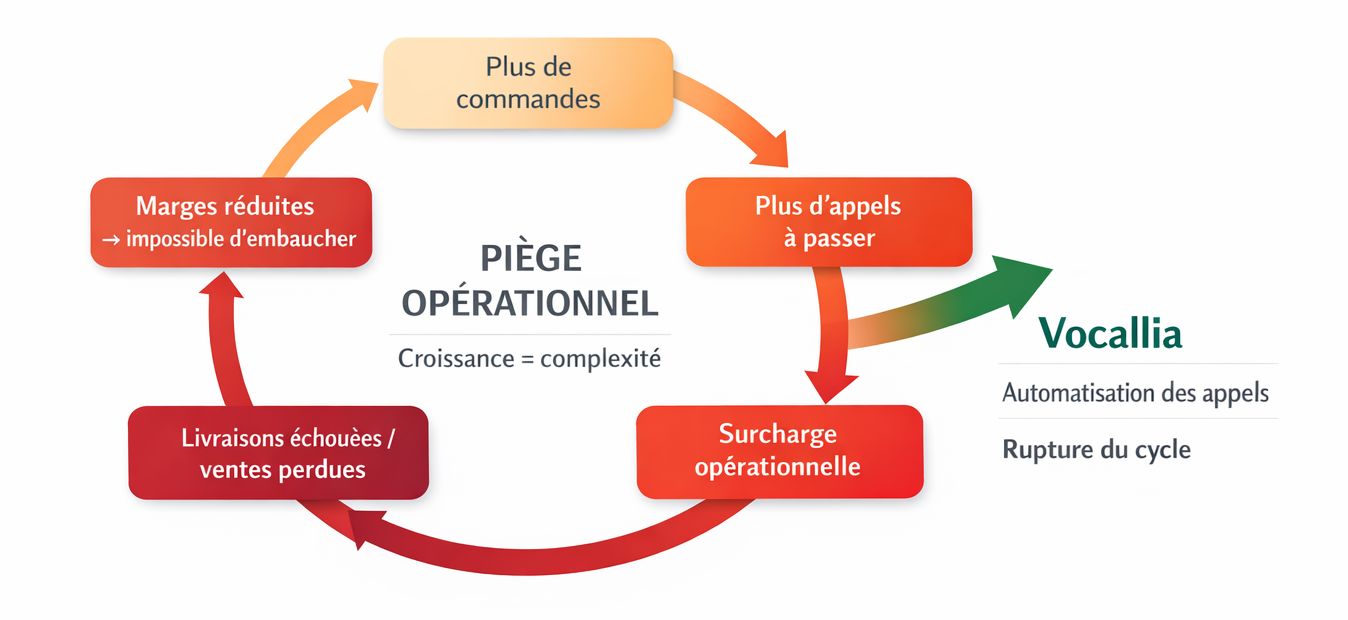
\includegraphics[width=0.78\textwidth]{figures/cercle-vicieux-marchand.png}
    \caption{Le cercle vicieux du marchand e-commerce sans automatisation}
    \label{fig:cercle-vicieux}
\end{figure}

Le positionnement ROI de Vocallia repose sur deux axes complémentaires~: la réduction des coûts directs mesurables (salaire, retours logistiques) et la libération du temps stratégique du dirigeant --- argument décisif dans un segment où la surcharge opérationnelle constitue le principal frein à la croissance.

\textit{Source~: INS, Enquête sur la population et l'emploi, 2024~; MDWEB, Baromètre e-commerce vague~4, 2023.}

%%%%%%%%%%%%%%%%%%%%%%%%%%%%%%%%%%%%%%%%%%%%%%%%%%%%%%%%%%%%%%%%%%%%%%%%%%%
\subsection{Environnement technologique}
\label{section2.1.4}
%%%%%%%%%%%%%%%%%%%%%%%%%%%%%%%%%%%%%%%%%%%%%%%%%%%%%%%%%%%%%%%%%%%%%%%%%%%

Le marché mondial de l'IA conversationnelle atteindra 41,39~milliards de dollars d'ici 2030, depuis 11,58~milliards en 2024 (CAGR de 23,7~\%, Grand View Research, 2024). Le segment des agents vocaux IA croît encore plus vite~: 34,8~\% par an entre 2024 et 2034 (Market.us, 2024), confirmé par Technavio à 37,2~\% sur 2024-2029. Cette dynamique traduit non pas une mode, mais une transition technologique de fond dans la gestion de la relation client.

Cette transition est rendue possible par la conjonction de trois maturités techniques simultanées~: la reconnaissance vocale (STT), portée notamment par Whisper d'OpenAI --- avec des limites persistantes sur le darija qui constituent précisément la niche de Vocallia~; les modèles de langage (LLM) accessibles via API à coût décroissant~; et la synthèse vocale (TTS), dont la naturalité progresse rapidement. Les contraintes techniques résiduelles --- latence cible inférieure à 800~ms, gestion des hallucinations sur cas-limites --- sont gérées par une architecture de \emph{fallback} vers un agent humain et par un périmètre fonctionnel volontairement restreint au lancement.

Vocallia entre sur le marché au moment précis où la technologie vocale IA est suffisamment mature pour être viable, et suffisamment récente pour que le marché local soit encore vierge --- ce qui constitue la définition même d'un point d'entrée optimal. Dans 18 à 24~mois, cet avantage temporel se réduira~: soit les API globales progresseront significativement sur l'arabe dialectal, soit des concurrents locaux auront émergé. Chaque mois d'avance se traduit en données propriétaires accumulées, en clients intégrés et en réputation marché --- trois actifs que nul entrant futur ne pourra racheter. L'urgence d'exécution n'est donc pas tactique~: elle est technologiquement et concurrentiellement fondée.

\textit{Source~: Grand View Research, Conversational AI Market Report, 2024~; Market.us, Voice AI Agents Market, 2024~; Technavio, Voice AI Agents Market Forecast 2025-2029.}

%%%%%%%%%%%%%%%%%%%%%%%%%%%%%%%%%%%%%%%%%%%%%%%%%%%%%%%%%%%%%%%%%%%%%%%%%%%
\subsection{Environnement écologique}
\label{section2.1.5}
%%%%%%%%%%%%%%%%%%%%%%%%%%%%%%%%%%%%%%%%%%%%%%%%%%%%%%%%%%%%%%%%%%%%%%%%%%%

Le modèle opérationnel de Vocallia génère un bilan environnemental indirect favorable~: en réduisant les expéditions non confirmées, la solution diminue les émissions logistiques liées aux retours. Le recours à une infrastructure cloud mutualisée produit une empreinte carbone par interaction nettement inférieure à celle d'un centre d'appels physique. À terme, un déploiement sur serveurs locaux (OVH Tunisie ou infrastructure privée) est envisagé pour les secteurs sensibles, renforçant simultanément la souveraineté des données et la maîtrise de l'empreinte numérique. Cet impact environnemental positif constitue par ailleurs un levier d'éligibilité aux programmes de financement à dimension ESG --- critère d'accès croissant aux appels à projets institutionnels et aux fonds d'investissement à impact.

%%%%%%%%%%%%%%%%%%%%%%%%%%%%%%%%%%%%%%%%%%%%%%%%%%%%%%%%%%%%%%%%%%%%%%%%%%%
\subsection{Environnement légal --- Éthique de l'IA vocale et protection des données}
\label{section2.1.6}
%%%%%%%%%%%%%%%%%%%%%%%%%%%%%%%%%%%%%%%%%%%%%%%%%%%%%%%%%%%%%%%%%%%%%%%%%%%

Vocallia opère dans un espace réglementaire en cours de structuration. Trois principes éthiques et légaux sont intégrés dès la conception du produit, sans compromis. \textbf{Premièrement}, le consentement explicite~: chaque appel s'ouvre par une annonce claire de sa nature automatisée, conformément à la loi n\degre{}2004-63 --- protection simultanée du client final et du marchand contre tout risque de contentieux. \textbf{Deuxièmement}, la minimisation des données~: conservation des enregistrements vocaux et transcriptions limitée à 30~jours par défaut, avec suppression sur demande. \textbf{Troisièmement}, le droit au transfert humain~: chaque scénario d'appel intègre un mécanisme de redirection vers un agent humain dès que la requête dépasse les capacités du système, garantissant la qualité de l'expérience sans risque de blocage.

À mesure que les régulations autour de l'IA vocale se durciront --- tendance mondiale irréversible --- les acteurs n'ayant pas intégré ces exigences dès l'origine subiront des coûts de mise en conformité élevés et des délais d'adaptation. Vocallia, ayant construit sa conformité comme fondation opérationnelle et non comme ajout tardif, transforme chaque renforcement réglementaire futur en avantage concurrentiel supplémentaire vis-à-vis des entrants moins rigoureux.

\begin{figure}[H]
    \centering
    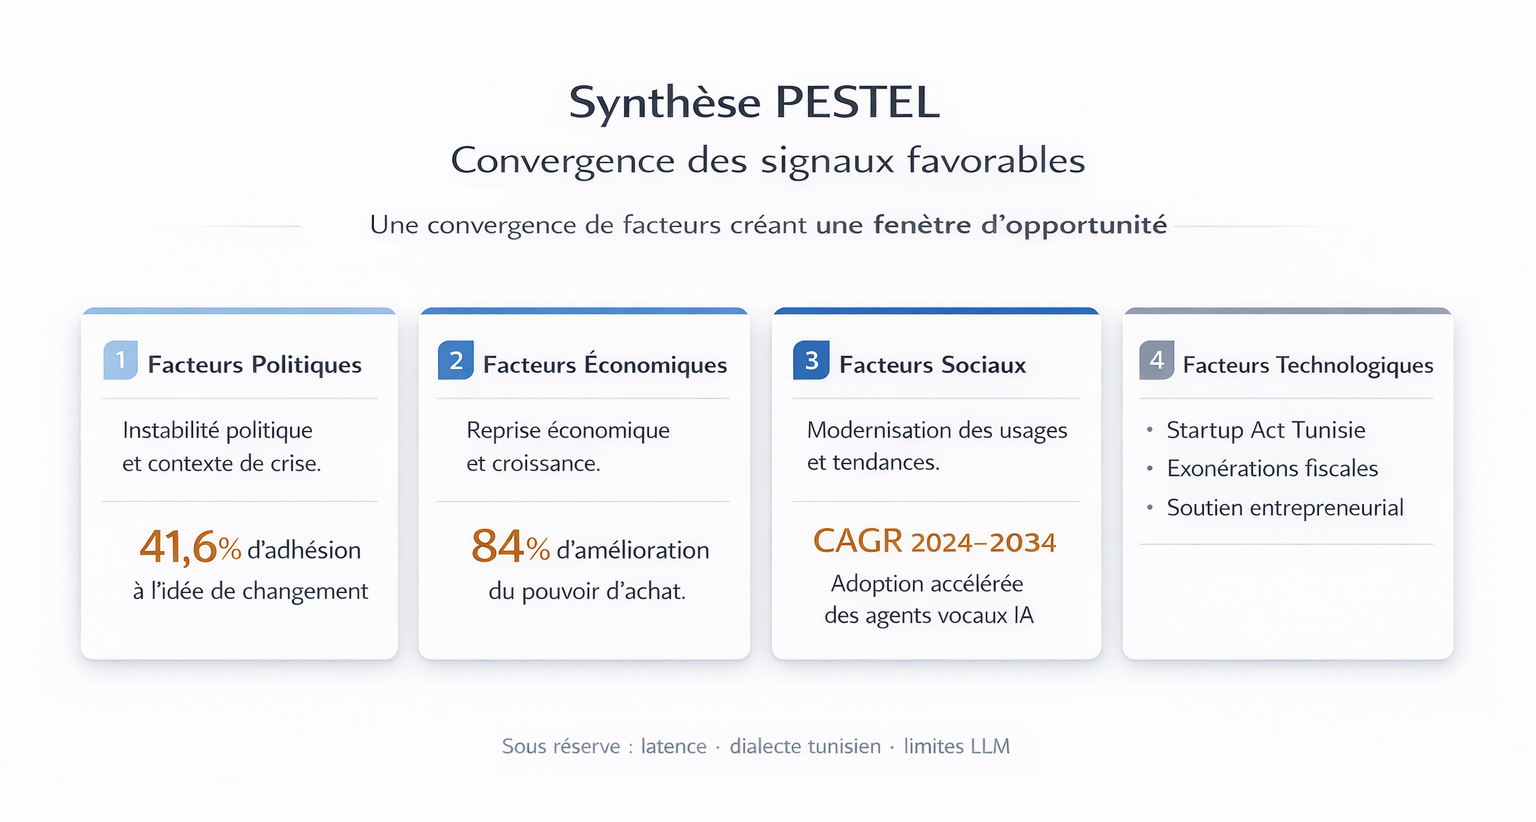
\includegraphics[width=0.95\textwidth]{figures/pestel-convergences.png}
    \caption{Synthèse PESTEL~: convergence des signaux favorables pour Vocallia}
    \label{fig:pestel-convergences}
\end{figure}

L'environnement macro étant caractérisé, il convient d'examiner la dynamique concurrentielle du secteur lui-même --- c'est l'objet de l'analyse sectorielle qui suit.

%%%%%%%%%%%%%%%%%%%%%%%%%%%%%%%%%%%%%%%%%%%%%%%%%%%%%%%%%%%%%%%%%%%%%%%%%%%
\section{Analyse sectorielle --- Les cinq forces de Porter}
\label{section2.2}
%%%%%%%%%%%%%%%%%%%%%%%%%%%%%%%%%%%%%%%%%%%%%%%%%%%%%%%%%%%%%%%%%%%%%%%%%%%

Appliqué au marché de l'automatisation vocale B2B en Tunisie, le modèle de Porter (1979) révèle un secteur fondamentalement attractif à court terme, dont les vulnérabilités sont identifiées, gérées et en partie transformées en leviers stratégiques par Vocallia. La figure~\ref{fig:porter-five-forces} synthétise le niveau de chaque force~; les sous-sections qui suivent en détaillent les mécanismes.

\begin{figure}[H]
    \centering
    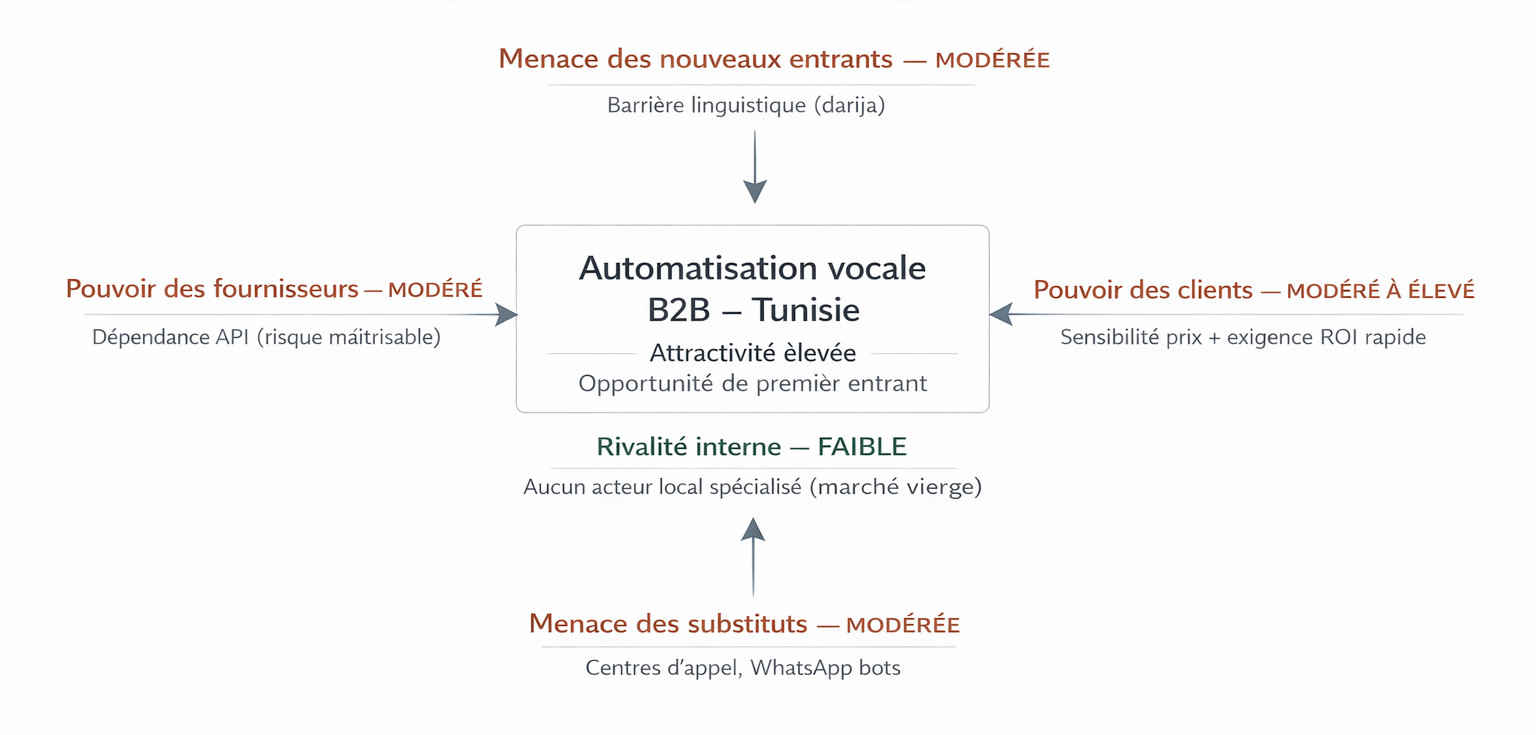
\includegraphics[width=0.82\textwidth]{figures/porter-five-forces-vocallia.png}
    \caption{Synthèse des cinq forces de Porter --- Marché de l'automatisation vocale B2B en Tunisie}
    \label{fig:porter-five-forces}
\end{figure}

%%%%%%%%%%%%%%%%%%%%%%%%%%%%%%%%%%%%%%%%%%%%%%%%%%%%%%%%%%%%%%%%%%%%%%%%%%%
\subsection{Force 1 --- Rivalité interne (faible)}
\label{section2.2.1}
%%%%%%%%%%%%%%%%%%%%%%%%%%%%%%%%%%%%%%%%%%%%%%%%%%%%%%%%%%%%%%%%%%%%%%%%%%%

Aucun acteur local ne propose aujourd'hui de solution d'agent vocal IA spécialisée pour les e-commerçants tunisiens. La rivalité directe est nulle. Cette situation crée une opportunité de premier entrant dont la valeur est inversement proportionnelle à sa durée~: dans un horizon de 18 à 36~mois, si Vocallia démontre la viabilité du modèle, des concurrents locaux ou des solutions internationales adaptées émergeront. La stratégie de défense est claire~: convertir cette avance temporelle en actifs durables --- base clients active, corpus de données propriétaires, réputation marché. Le premier acteur à atteindre la masse critique crédentielle --- 30 à 50~clients actifs, plusieurs dizaines de milliers d'appels traités, intégrations déployées --- s'imposera comme standard de référence et bénéficiera d'un effet réseau de réputation que la concurrence ne pourra dupliquer qu'au prix d'un investissement considérable.

%%%%%%%%%%%%%%%%%%%%%%%%%%%%%%%%%%%%%%%%%%%%%%%%%%%%%%%%%%%%%%%%%%%%%%%%%%%
\subsection{Force 2 --- Menace des nouveaux entrants (modérée)}
\label{section2.2.2}
%%%%%%%%%%%%%%%%%%%%%%%%%%%%%%%%%%%%%%%%%%%%%%%%%%%%%%%%%%%%%%%%%%%%%%%%%%%

Les barrières à l'entrée sont réelles mais non permanentes. La plus significative est linguistique~: la maîtrise du darija --- dialecte non standardisé, caractérisé par un code-switching arabe/français dense et une variabilité phonologique régionale --- exige des données d'entraînement locales spécifiques qu'aucun acteur global ne possède. Le risque principal est la désintermédiation technologique~: si des fournisseurs globaux comme OpenAI améliorent leur couverture de l'arabe dialectal, la barrière linguistique s'érode partiellement. Ce risque est contenu par l'accumulation active d'un corpus propriétaire de données vocales en darija --- actif immatériel non reproductible sans historique opérationnel local.

La barrière linguistique constitue ainsi le point de départ, non le point d'arrivée de la défendabilité de Vocallia. Sa pérennité dépend de la capacité à la transformer en un fossé de données auto-entretenu, dont le mécanisme de \emph{flywheel} est détaillé en figure~\ref{fig:flywheel-vocallia}. L'apprentissage continu produit un effet de composition~: chaque itération du modèle améliore la capacité du système à extraire de la valeur des données futures, créant un écart de performance qui s'accélère plutôt qu'il ne se stabilise. Un concurrent entrant dans 24~mois ne pourra pas acheter cet historique --- il devra le reconstruire entièrement, avec les erreurs et le temps que cela implique.

%%%%%%%%%%%%%%%%%%%%%%%%%%%%%%%%%%%%%%%%%%%%%%%%%%%%%%%%%%%%%%%%%%%%%%%%%%%
\subsection{Force 3 --- Pouvoir de négociation des clients (modéré à élevé)}
\label{section2.2.3}
%%%%%%%%%%%%%%%%%%%%%%%%%%%%%%%%%%%%%%%%%%%%%%%%%%%%%%%%%%%%%%%%%%%%%%%%%%%

Les e-commerçants tunisiens sont des PME à forte sensibilité prix et à exigence de ROI rapide. Ce pouvoir de négociation est toutefois limité par l'absence d'alternative directe~: sans concurrent comparable, le client ne peut pas «~faire jouer la concurrence~». La stratégie d'entrée de Vocallia --- pilote à faible engagement initial --- réduit le risque perçu et abaisse la friction à l'adoption. Une fois l'intégration technique déployée (connexion API, scripts personnalisés, synchronisation des commandes), les coûts de changement deviennent significatifs~: migrer vers une solution concurrente implique de tout recommencer --- formation, paramétrage, historique des appels, personnalisation des flux. Ces \emph{switching costs} ne sont pas statiques~: ils s'accroissent avec la durée de la relation, à mesure que l'historique d'appels et les données de performance accumulées deviennent des actifs opérationnels dont le client dépend quotidiennement.

%%%%%%%%%%%%%%%%%%%%%%%%%%%%%%%%%%%%%%%%%%%%%%%%%%%%%%%%%%%%%%%%%%%%%%%%%%%
\subsection{Force 4 --- Pouvoir de négociation des fournisseurs (modéré)}
\label{section2.2.4}
%%%%%%%%%%%%%%%%%%%%%%%%%%%%%%%%%%%%%%%%%%%%%%%%%%%%%%%%%%%%%%%%%%%%%%%%%%%

Vocallia dépend de fournisseurs d'API globaux (OpenAI, ElevenLabs, Twilio) dont les tarifs sont standardisés et peu négociables en phase d'amorçage. Ce risque est contenu par une architecture multi-fournisseurs permettant la substitution rapide en cas de hausse tarifaire ou d'interruption de service. À mesure que le volume d'appels croît, les économies d'échelle sur les API réduisent le coût par appel et élargissent les marges opérationnelles. La dépendance fournisseurs est donc une contrainte d'amorçage, gérée par \emph{design}, qui se renverse avec la croissance~: le \emph{scaling} du volume transforme Vocallia en client significatif pour ses \emph{providers}, ouvrant des conditions préférentielles et améliorant durablement les marges.

%%%%%%%%%%%%%%%%%%%%%%%%%%%%%%%%%%%%%%%%%%%%%%%%%%%%%%%%%%%%%%%%%%%%%%%%%%%
\subsection{Force 5 --- Menace des substituts (modérée)}
\label{section2.2.5}
%%%%%%%%%%%%%%%%%%%%%%%%%%%%%%%%%%%%%%%%%%%%%%%%%%%%%%%%%%%%%%%%%%%%%%%%%%%

Trois catégories de substituts sont identifiables~: les agents humains internes (coût élevé, scalabilité nulle), les centres d'appels externalisés (coût variable élevé, perte de contrôle relationnel), et les chatbots textuels WhatsApp/Messenger (déploiement facile, mais canal non équivalent au vocal pour la confirmation de commandes). Aucun ne combine scalabilité illimitée, disponibilité 24h/24, coût faible par interaction et conversation vocale en dialecte tunisien. Les chatbots WhatsApp Business constituent la menace la plus crédible à court terme, mais leur limite est structurelle~: le canal textuel génère des taux de réponse et de conversion inférieurs au vocal, où la voix --- même synthétisée --- crée un niveau d'engagement que le texte ne peut reproduire. Vocallia devra démontrer cette supériorité par des données chiffrées lors de la phase pilote.

\begin{tcolorbox}[colback=gray!8, colframe=gray!50, title=\textbf{Attractivité sectorielle --- Verdict Porter}, fonttitle=\bfseries]
\textbf{Le secteur est fondamentalement attractif aujourd'hui, et cette attractivité est temporaire.} Rivalité directe nulle, barrière linguistique défendable, substituts incomplets~: les conditions d'entrée sont exceptionnellement favorables. Les deux risques à surveiller --- désintermédiation technologique et émergence de nouveaux entrants capitalisés --- partagent la même réponse stratégique~: l'accumulation accélérée de données propriétaires et de clients actifs. Chaque jour d'opération construit une position que nul entrant futur ne pourra reprendre sans investir plusieurs fois la mise initiale de Vocallia.
\end{tcolorbox}

L'attractivité sectorielle étant établie, la question suivante est celle de la taille du marché capturable --- et de la trajectoire commerciale réaliste à trois ans.

%%%%%%%%%%%%%%%%%%%%%%%%%%%%%%%%%%%%%%%%%%%%%%%%%%%%%%%%%%%%%%%%%%%%%%%%%%%
\section{Quantification du marché cible --- Cadre TAM / SAM / SOM}
\label{section2.3}
%%%%%%%%%%%%%%%%%%%%%%%%%%%%%%%%%%%%%%%%%%%%%%%%%%%%%%%%%%%%%%%%%%%%%%%%%%%

Le cadre TAM/SAM/SOM permet de distinguer le potentiel théorique d'un marché de la cible commerciale réaliste à court terme. Les estimations ci-après reposent sur les données officielles de la BCT (2024) et les résultats de l'étude exploratoire Muvaka (avril 2025). Elles sont volontairement conservatrices~: elles excluent le commerce informel via réseaux sociaux et l'extension à d'autres secteurs, qui constituent des vecteurs d'\emph{upside} non intégrés dans les projections de base.

%%%%%%%%%%%%%%%%%%%%%%%%%%%%%%%%%%%%%%%%%%%%%%%%%%%%%%%%%%%%%%%%%%%%%%%%%%%
\subsection{TAM --- Marché total adressable}
\label{section2.3.1}
%%%%%%%%%%%%%%%%%%%%%%%%%%%%%%%%%%%%%%%%%%%%%%%%%%%%%%%%%%%%%%%%%%%%%%%%%%%

Le TAM de Vocallia recouvre l'ensemble des entités tunisiennes ayant un besoin régulier et récurrent d'appels clients sortants. La BCT recensait 1\,126 sites marchands actifs en 2024. Le baromètre MDWEB (vague~4, 2023) suggère que le volume des transactions informelles via réseaux sociaux serait d'une ampleur comparable au marché formel --- hypothèse cohérente avec la structure duale du commerce tunisien. En intégrant les e-commerçants informels, les agences, cabinets médicaux, services de livraison et centres de formation, le TAM est estimé à \textbf{plus de 8\,000 entités potentielles}. L'architecture modulaire de la solution --- scripts paramétrables par secteur --- permet d'adresser ces verticaux sans refonte technologique majeure, transformant le TAM d'une estimation statique en un marché expansible par \emph{design}.

\textit{Source~: BCT, Bulletin sur les paiements 2024~; MDWEB, Baromètre e-commerce vague~4, 2023.}

%%%%%%%%%%%%%%%%%%%%%%%%%%%%%%%%%%%%%%%%%%%%%%%%%%%%%%%%%%%%%%%%%%%%%%%%%%%
\subsection{SAM --- Marché serviceable}
\label{section2.3.2}
%%%%%%%%%%%%%%%%%%%%%%%%%%%%%%%%%%%%%%%%%%%%%%%%%%%%%%%%%%%%%%%%%%%%%%%%%%%

Le SAM est délimité aux e-commerçants dont la volumétrie d'appels justifie économiquement le recours à une solution SaaS B2B, et dont la structure organisationnelle est suffisamment formalisée pour l'adopter. Les données Muvaka (22 répondants, avril 2025) indiquent que 63,7~\% des répondants traitent plus de 5 appels de confirmation par jour --- seuil à partir duquel l'automatisation devient rentable dès le premier mois. En extrapolant prudemment à la base officielle de 1\,126 marchands actifs (BCT 2024), le SAM est estimé entre \textbf{700 et 900 e-commerçants}. Ce chiffre sous-estime vraisemblablement le marché réel, dans la mesure où il exclut l'ensemble du commerce informel.

%%%%%%%%%%%%%%%%%%%%%%%%%%%%%%%%%%%%%%%%%%%%%%%%%%%%%%%%%%%%%%%%%%%%%%%%%%%
\subsection{SOM --- Marché capturable à 3 ans}
\label{section2.3.3}
%%%%%%%%%%%%%%%%%%%%%%%%%%%%%%%%%%%%%%%%%%%%%%%%%%%%%%%%%%%%%%%%%%%%%%%%%%%

Le SOM représente la cible commerciale réaliste à trois ans. L'objectif est de capter entre 5 et 8~\% du SAM, soit \textbf{40 à 70 clients actifs en fin d'année~3}. À un revenu mensuel récurrent moyen de 120~DT par client, le SOM se traduit par un chiffre d'affaires annuel récurrent cible entre \textbf{57\,600~DT et 100\,800~DT} --- avant toute extension sectorielle.

Ces projections sont délibérément prudentes~: elles reposent sur un rythme d'acquisition de 1 à 2 nouveaux clients par mois, sans croissance organique par recommandation. Le SOM projeté représente la borne basse crédible d'un scénario sans levier externe, et constitue le socle à partir duquel chaque extension sectorielle --- santé, immobilier, logistique, formation --- représente un multiplicateur de revenus sans coût marginal élevé. À horizon cinq ans, la confirmation de commandes constitue le cas d'usage d'ancrage --- le point d'entrée à partir duquel Vocallia a vocation à devenir une infrastructure conversationnelle complète~: relance de paniers abandonnés, enquêtes de satisfaction, prise de rendez-vous médicaux, qualification de leads immobiliers. Chaque vertical ajouté réutilise le même socle technologique, le même corpus linguistique et la même base de clients, transformant un outil mono-usage en plateforme à revenus composés.

\begin{figure}[H]
    \centering
    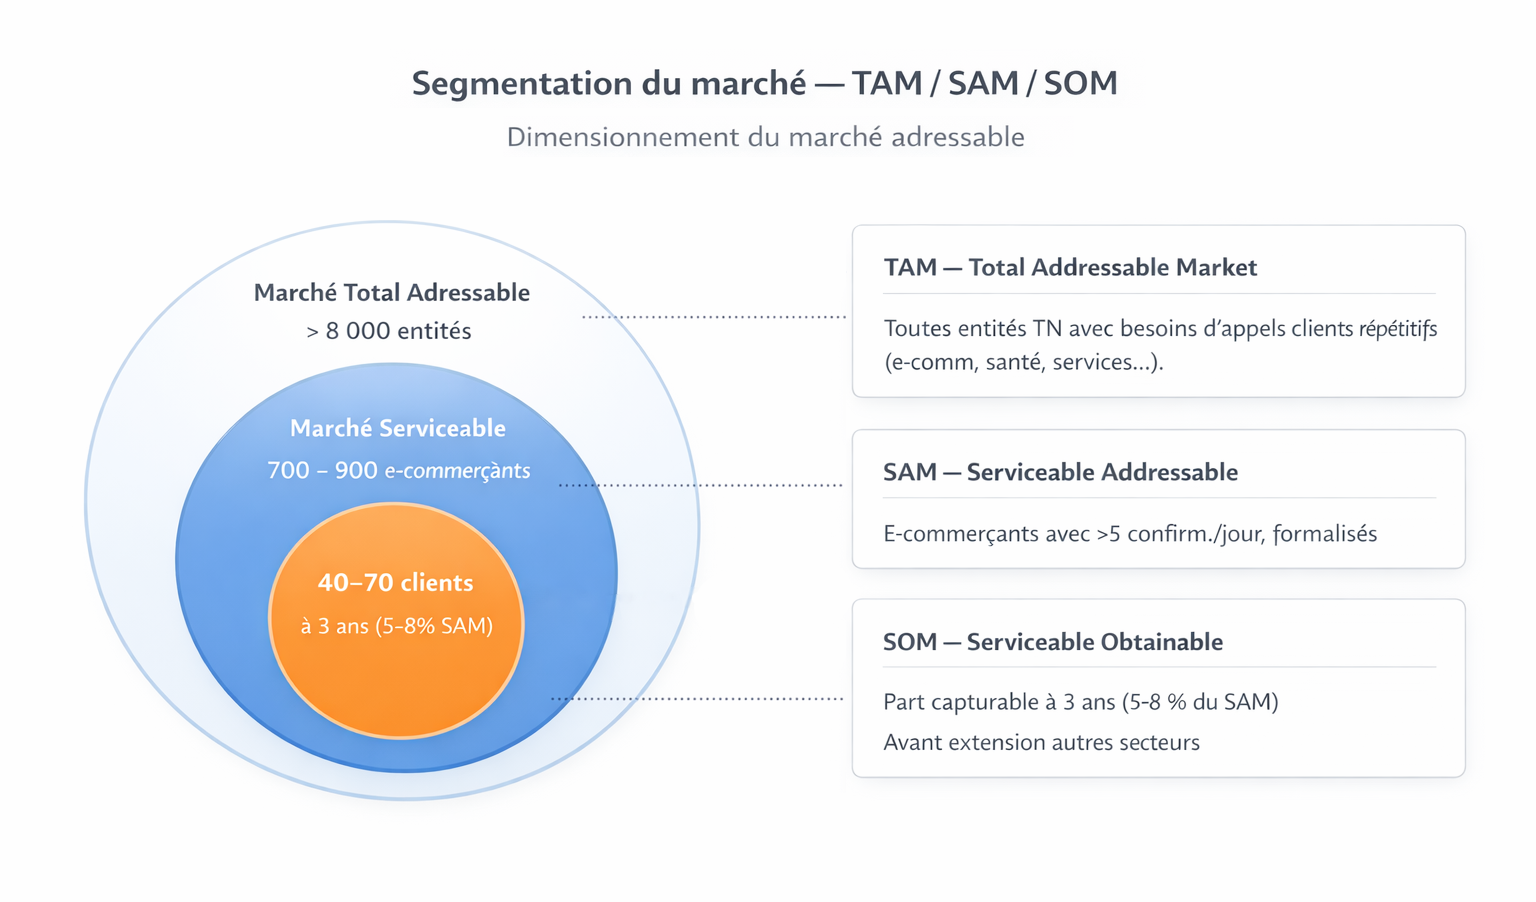
\includegraphics[width=\textwidth]{figures/tam-sam-som-vocallia.png}
    \caption{Représentation visuelle du TAM, SAM et SOM de Vocallia (2025)}
    \label{fig:tam-sam-som-vocallia}
\end{figure}

Les estimations quantitatives qui précèdent reposent sur des données secondaires. Pour les confronter à la réalité du terrain, une étude exploratoire a été conduite directement auprès des e-commerçants.

%%%%%%%%%%%%%%%%%%%%%%%%%%%%%%%%%%%%%%%%%%%%%%%%%%%%%%%%%%%%%%%%%%%%%%%%%%%
\section{Étude exploratoire terrain --- Phase Muvaka (avril 2025)}
\label{section2.4}
%%%%%%%%%%%%%%%%%%%%%%%%%%%%%%%%%%%%%%%%%%%%%%%%%%%%%%%%%%%%%%%%%%%%%%%%%%%

Avant de figer l'identité commerciale sous le nom Vocallia, une phase d'exploration de marché a été conduite en avril 2025 sous la marque de test Muvaka. Ce choix méthodologique, inspiré des pratiques du \emph{Lean Startup} (Ries, 2011), visait à tester la réceptivité du marché sans biais d'identité de marque, et à recueillir des données primaires directement auprès des e-commerçants tunisiens dans leur réalité opérationnelle.

Avec 22 répondants, les résultats constituent une étude exploratoire qualitative, non une validation statistique généralisable. Leur valeur réside dans la cohérence interne des signaux observés et leur convergence avec les données macroéconomiques établies dans les sections précédentes.

%%%%%%%%%%%%%%%%%%%%%%%%%%%%%%%%%%%%%%%%%%%%%%%%%%%%%%%%%%%%%%%%%%%%%%%%%%%
\subsection{Dispositif de collecte}
\label{section2.4.1}
%%%%%%%%%%%%%%%%%%%%%%%%%%%%%%%%%%%%%%%%%%%%%%%%%%%%%%%%%%%%%%%%%%%%%%%%%%%

Le dispositif combinait une \emph{landing page} de capture d'intérêt, un formulaire structuré de 9 questions et deux campagnes Meta Ads (Facebook / Instagram) complémentaires, déployées sur 7 jours avec un budget total de 20~euros --- démarche de validation à coût marginal, cohérente avec le stade d'amorçage.

%%%%%%%%%%%%%%%%%%%%%%%%%%%%%%%%%%%%%%%%%%%%%%%%%%%%%%%%%%%%%%%%%%%%%%%%%%%
\subsection{Résultats des campagnes Meta Ads}
\label{section2.4.2}
%%%%%%%%%%%%%%%%%%%%%%%%%%%%%%%%%%%%%%%%%%%%%%%%%%%%%%%%%%%%%%%%%%%%%%%%%%%

Deux campagnes aux objectifs complémentaires ont mesuré à la fois l'attractivité du message et la capacité à générer des leads qualifiés.

\begin{figure}[H]
    \centering
    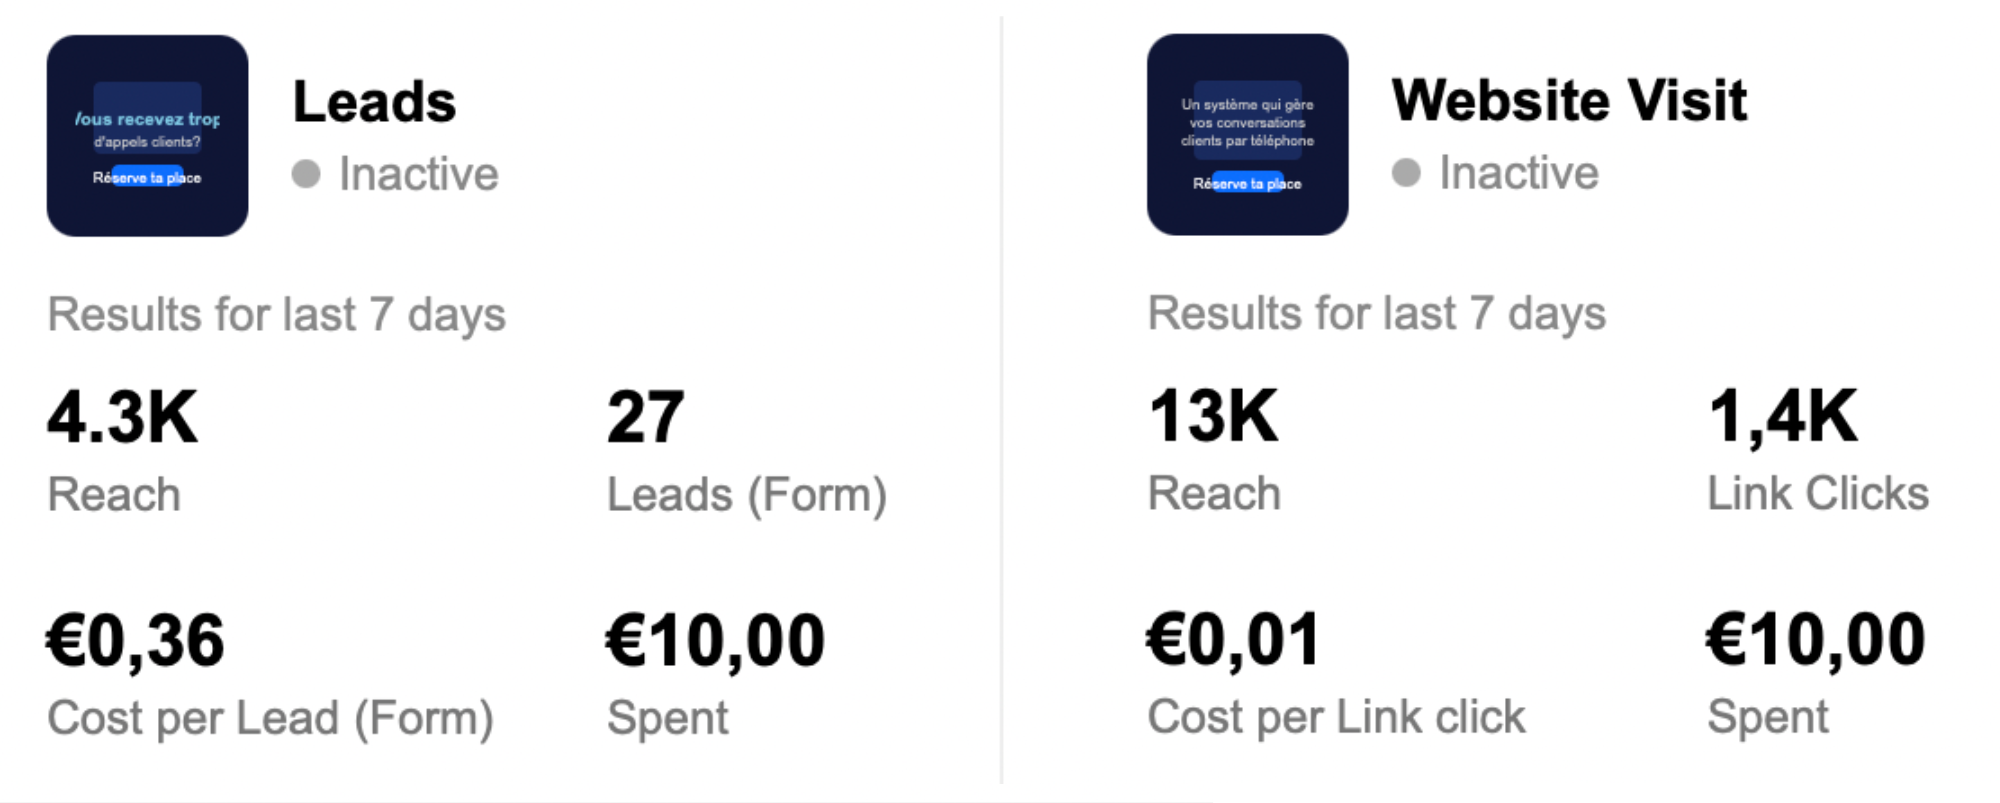
\includegraphics[width=0.78\textwidth]{figures/meta-ads-results.png}
    \caption{Résultats des campagnes Meta Ads --- Phase Muvaka (7 jours)}
    \label{fig:meta-ads-results}
\end{figure}

\textbf{Lecture analytique.} Le taux de clic de 10,9~\% (clics/\emph{reach}) sur la campagne \emph{Website Visit} dépasse de 7 à 20 fois les benchmarks B2B observés sur Meta Ads (0,5 -- 1,5~\%)~: c'est un signal de résonance forte du message auprès de l'audience ciblée. Le coût par lead de 0,36~\euro{} représente moins de 10~\% des moyennes B2B sectorielles (3 -- 15~\euro{}), indiquant une adéquation précise entre le ciblage et la douleur adressée. Ces résultats doivent être interprétés avec la prudence imposée par le budget limité et la durée courte de la campagne --- ils constituent néanmoins des signaux d'adéquation marché-message parmi les plus favorables qu'une phase exploratoire puisse produire à ce niveau de coût.

%%%%%%%%%%%%%%%%%%%%%%%%%%%%%%%%%%%%%%%%%%%%%%%%%%%%%%%%%%%%%%%%%%%%%%%%%%%
\subsection{Analyse des résultats du formulaire (22 répondants, e-commerçants actifs)}
\label{section2.4.3}
%%%%%%%%%%%%%%%%%%%%%%%%%%%%%%%%%%%%%%%%%%%%%%%%%%%%%%%%%%%%%%%%%%%%%%%%%%%

Le formulaire ciblait quatre dimensions~: profil du répondant, réalité du problème opérationnel, réceptivité à la solution et sensibilité prix.

\begin{table}[H]
\centering
\caption{Résultats du formulaire de recherche Muvaka --- 22 répondants}
\smallskip
\begin{tabular}{|p{2.8cm}|p{4.2cm}|p{4.8cm}|}
\hline
\textbf{Dimension} & \textbf{Résultat observé} & \textbf{Interprétation stratégique} \\
\hline
Ancienneté & 68,2~\% actifs depuis 3 ans ou plus & Marchands expérimentés~: ils connaissent le problème, ils ont déjà tout essayé \\
\hline
Volume appels/jour & 54,6~\% déclarent 6 appels ou plus & Charge opérationnelle récurrente, seuil de rentabilité de l'automatisation atteint \\
\hline
Gestion des appels & 52,4~\% par le gérant, 42,9~\% par un employé & Coût d'opportunité maximal~: ressources décisionnelles mobilisées sur du répétitif \\
\hline
Perte d'opportunités & \textbf{77,3~\% déclarent avoir perdu des ventes} & La friction opérationnelle se traduit directement en chiffre d'affaires perdu \\
\hline
Intérêt IA dialecte TN & 85~\% score 4 ou 5/5 & Réceptivité forte --- la barrière n'est pas culturelle mais technologique \\
\hline
Disposition à tester & \textbf{90,9~\% répondent Oui à un pilote} & Risque commercial d'acquisition quasi nul en phase de lancement \\
\hline
Sensibilité prix & 40,9~\% acceptent 50--150 DT/mois & Zone de pricing viable, cohérente avec le modèle SaaS projeté \\
\hline
\end{tabular}
\end{table}


Trois chiffres concentrent l'essentiel de la validation terrain. La figure~\ref{fig:kpi-muvaka} les isole pour en faire ressortir la force~: problème confirmé, solution désirée, adoption acquise.

\begin{figure}[H]
    \centering
    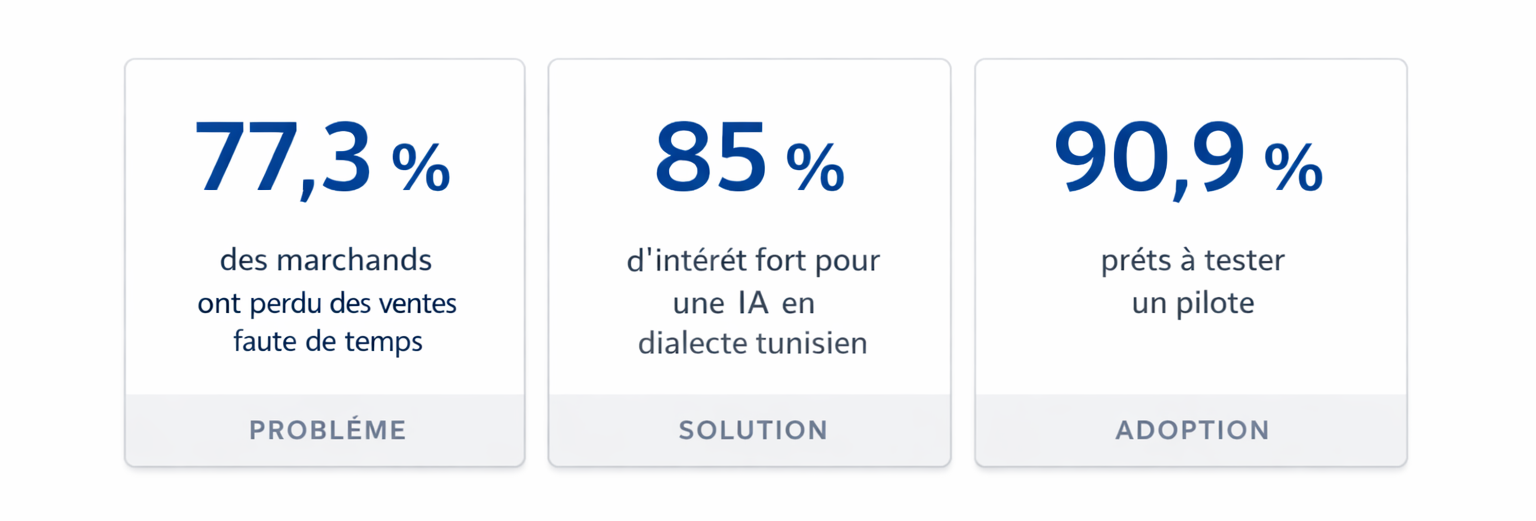
\includegraphics[width=0.95\textwidth]{figures/kpi-muvaka-triptyque.png}
    \caption{Triptyque de validation Muvaka --- Les trois signaux décisifs}
    \label{fig:kpi-muvaka}
\end{figure}

Le taux de 77,3~\% de marchands déclarant avoir perdu des ventes faute de temps transforme un problème d'efficacité en un \textbf{problème de chiffre d'affaires directement quantifiable} --- l'argument ROI le plus puissant disponible en démonstration B2B. Associé à 90,9~\% de disposition à tester un pilote, ce résultat révèle un marché non pas à convaincre, mais à équiper.

%%%%%%%%%%%%%%%%%%%%%%%%%%%%%%%%%%%%%%%%%%%%%%%%%%%%%%%%%%%%%%%%%%%%%%%%%%%
\subsection{Analyse des verbatims --- expression spontanée du problème}
\label{section2.4.4}
%%%%%%%%%%%%%%%%%%%%%%%%%%%%%%%%%%%%%%%%%%%%%%%%%%%%%%%%%%%%%%%%%%%%%%%%%%%

La question ouverte «~Quel est votre principal problème avec les appels clients~?~» (17 répondants) a généré des réponses spontanées en dialecte tunisien d'une clarté saisissante.

\begin{table}[H]
\centering
\caption{Verbatims --- expression spontanée du problème (dialecte tunisien)}
\smallskip
\begin{tabular}{|p{3.5cm}|p{3.5cm}|p{4cm}|}
\hline
\textbf{Verbatim (dialecte)} & \textbf{Traduction} & \textbf{Friction identifiée} \\
\hline
\og{}Ma yahezouch alik baad l confirmation\fg{} & Le client ne répond plus après confirmation & Annulation post-confirmation~: coût double \\
\hline
\og{}Tadhi3 wakt\fg{} & Perte de temps significative & Coût d'opportunité chronique \\
\hline
\og{}Totlob barcha marrat ou inajim yenssel ba3d\fg{} & Trop de tentatives sans résultat & Joignabilité faible, épuisement opérationnel \\
\hline
\og{}Ki manakhlatsh njawb, il annule mayhezesh\fg{} & Si on ne répond pas, la commande est annulée & Perte directe de CA par défaut de réactivité \\
\hline
\og{}Sa3t ma yefhemkch kol mara w kifeh\fg{} & Qualité variable de chaque échange & Absence de standardisation, risque image \\
\hline
\end{tabular}
\end{table}


Ces cinq verbatims couvrent l'intégralité du spectre de la friction~: non-joignabilité, perte de temps, annulation post-confirmation, perte de CA par défaut de réactivité, et variabilité qualitative. Leur expression spontanée en darija confirme que Vocallia doit parler la langue du problème --- littéralement. La maîtrise du dialecte n'est pas une fonctionnalité~: c'est la condition de l'adoption. Ces témoignages révèlent en creux une vérité plus large~: la question pour ces marchands n'est plus de savoir \emph{s'ils} automatiseront la confirmation, mais \emph{quand} --- et avec quel outil.

Au total, l'étude Muvaka valide simultanément les trois hypothèses fondamentales de tout modèle d'investissement \emph{early-stage}~: le problème est réel et douloureux~; la solution est désirée~; le prix est acceptable. L'étape suivante est leur confirmation à plus grande échelle --- mais la direction est établie avec un niveau de certitude suffisant pour déclencher l'exécution.

\medskip
La demande étant validée par le terrain, il reste à établir que l'espace concurrentiel est effectivement vide --- et à comprendre pourquoi il l'est.

%%%%%%%%%%%%%%%%%%%%%%%%%%%%%%%%%%%%%%%%%%%%%%%%%%%%%%%%%%%%%%%%%%%%%%%%%%%
\section{Analyse concurrentielle --- Benchmark local et international}
\label{section2.5}
%%%%%%%%%%%%%%%%%%%%%%%%%%%%%%%%%%%%%%%%%%%%%%%%%%%%%%%%%%%%%%%%%%%%%%%%%%%

L'analyse concurrentielle est conduite à deux niveaux~: le marché tunisien, pour cartographier les alternatives existantes et leurs limites~; le marché international, pour situer Vocallia face aux solutions d'IA vocale de référence mondiale.

%%%%%%%%%%%%%%%%%%%%%%%%%%%%%%%%%%%%%%%%%%%%%%%%%%%%%%%%%%%%%%%%%%%%%%%%%%%
\subsection{Alternatives disponibles sur le marché tunisien}
\label{section2.5.1}
%%%%%%%%%%%%%%%%%%%%%%%%%%%%%%%%%%%%%%%%%%%%%%%%%%%%%%%%%%%%%%%%%%%%%%%%%%%

Trois catégories de solutions existent sur le marché tunisien~: agents humains internes, centres d'appels externalisés, et outils de messagerie automatisée. \textbf{Aucun acteur ne propose à ce jour d'agent vocal IA en dialecte tunisien pour les e-commerçants.} Cette lacune reflète la complexité linguistique du darija et l'absence jusqu'ici d'une équipe locale capable de l'adresser techniquement.

\begin{table}[H]
\centering
\caption{Comparaison des alternatives sur le marché tunisien}
\smallskip
\begin{tabular}{|p{3cm}|l|l|l|l|}
\hline
\textbf{Critère} & \textbf{Agents internes} & \textbf{Call centers} & \textbf{Chatbots} & \textbf{Vocallia} \\
\hline
Appel vocal sortant & Oui & Oui (humain) & Non & Oui (IA) \\
\hline
Dialecte tunisien & Oui & Oui (humain) & Partiel & Oui (natif) \\
\hline
Scalabilité & Très limitée & Limitée & Élevée & Élevée \\
\hline
Coût / appel & Élevé & Élevé & Très faible & Faible \\
\hline
Traçabilité & Faible & Faible & Modérée & Élevée \\
\hline
Disponibilité 24h/24 & Non & Non & Oui & Oui \\
\hline
\end{tabular}
\end{table}


%%%%%%%%%%%%%%%%%%%%%%%%%%%%%%%%%%%%%%%%%%%%%%%%%%%%%%%%%%%%%%%%%%%%%%%%%%%
\subsection{Benchmark international --- solutions Voice AI globales}
\label{section2.5.2}
%%%%%%%%%%%%%%%%%%%%%%%%%%%%%%%%%%%%%%%%%%%%%%%%%%%%%%%%%%%%%%%%%%%%%%%%%%%

Les plateformes d'agents vocaux IA internationales --- Bland.ai, Vapi.ai, Retell, ElevenLabs --- ont émergé ces deux dernières années, portées par la démocratisation des API de langage et de synthèse vocale. Elles constituent la référence technologique mondiale, mais aucune n'adresse le marché tunisien.

\begin{table}[H]
\centering
\caption{Benchmark international --- solutions Voice AI globales}
\smallskip
\begin{tabular}{|p{2.8cm}|l|l|l|l|l|}
\hline
\textbf{Critère} & \textbf{Bland.ai} & \textbf{Vapi.ai} & \textbf{Retell} & \textbf{ElevenLabs} & \textbf{Vocallia} \\
\hline
Dialecte arabe TN & Non & Non & Non & Partiel & Oui \\
\hline
Code-switching AR/FR & Non & Non & Non & Non & Oui \\
\hline
Coût / appel 2 min & 0,18~\$ & 0,14~\$ & 0,14~\$ & 0,24~\$ & 0,10~\$ \\
\hline
Déploiement local & Non & Non & Non & Non & Prévu \\
\hline
Support MENA/TN & Non & Non & Non & Non & Oui \\
\hline
Pricing PME en DT & Non & Non & Non & Non & Oui \\
\hline
\end{tabular}
\end{table}


La figure~\ref{fig:radar-positionnement} traduit visuellement la dominance de Vocallia sur l'ensemble des critères pertinents pour le marché tunisien. Les acteurs internationaux ne sont pas des concurrents directs --- ils sont des fournisseurs de technologie générique incapables d'adresser la dimension linguistique, opérationnelle et économique du marché local sans un investissement dédié qu'aucun d'eux n'a engagé.

\begin{figure}[H]
    \centering
    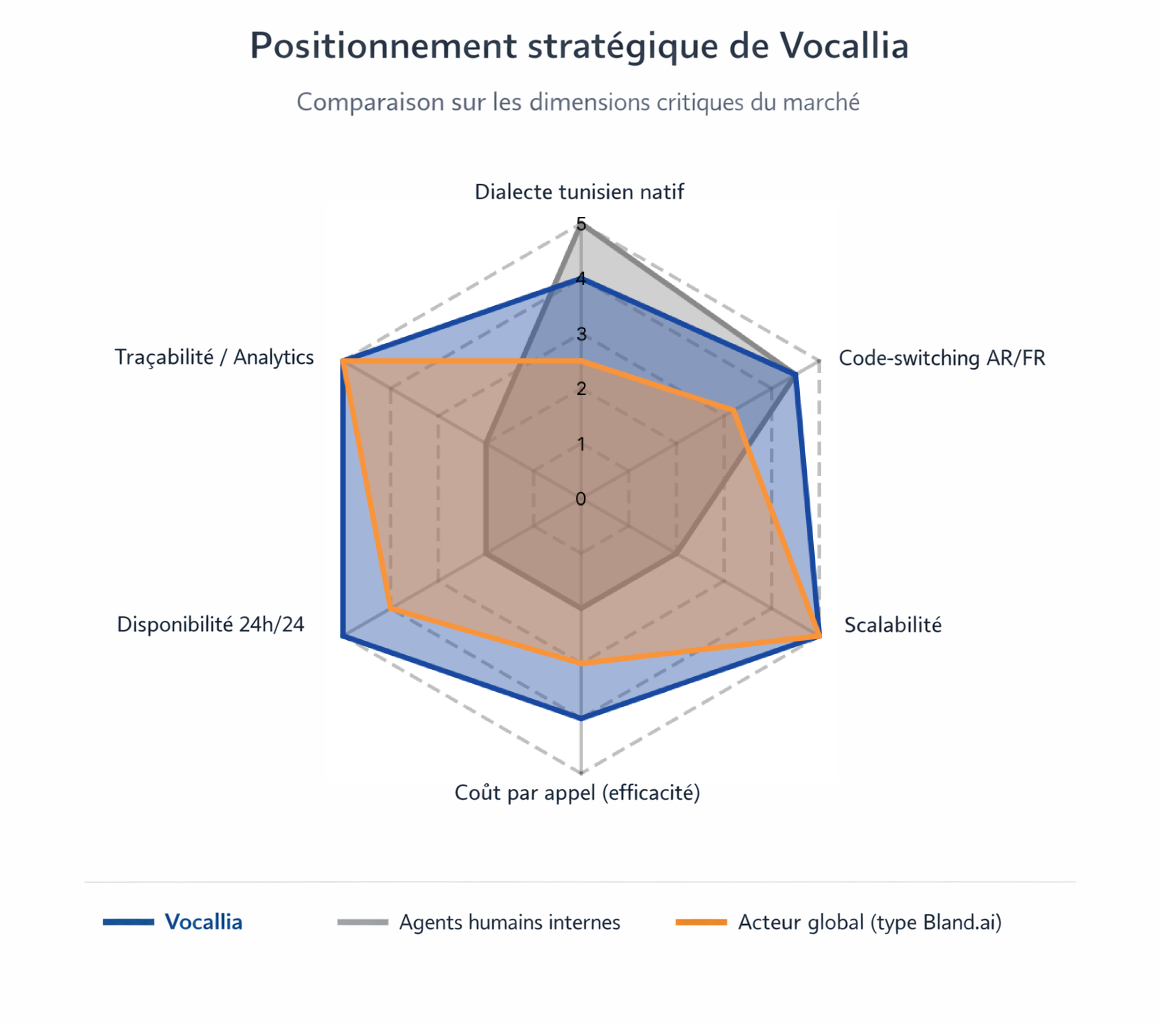
\includegraphics[width=0.75\textwidth]{figures/radar-positionnement-vocallia.png}
    \caption{Positionnement concurrentiel multidimensionnel --- Vocallia vs. alternatives}
    \label{fig:radar-positionnement}
\end{figure}

Le fossé concurrentiel qui en résulte repose sur quatre piliers auto-renforçants, dont le mécanisme central --- le \emph{flywheel} de données --- est représenté en figure~\ref{fig:flywheel-vocallia}.

\begin{figure}[H]
    \centering
    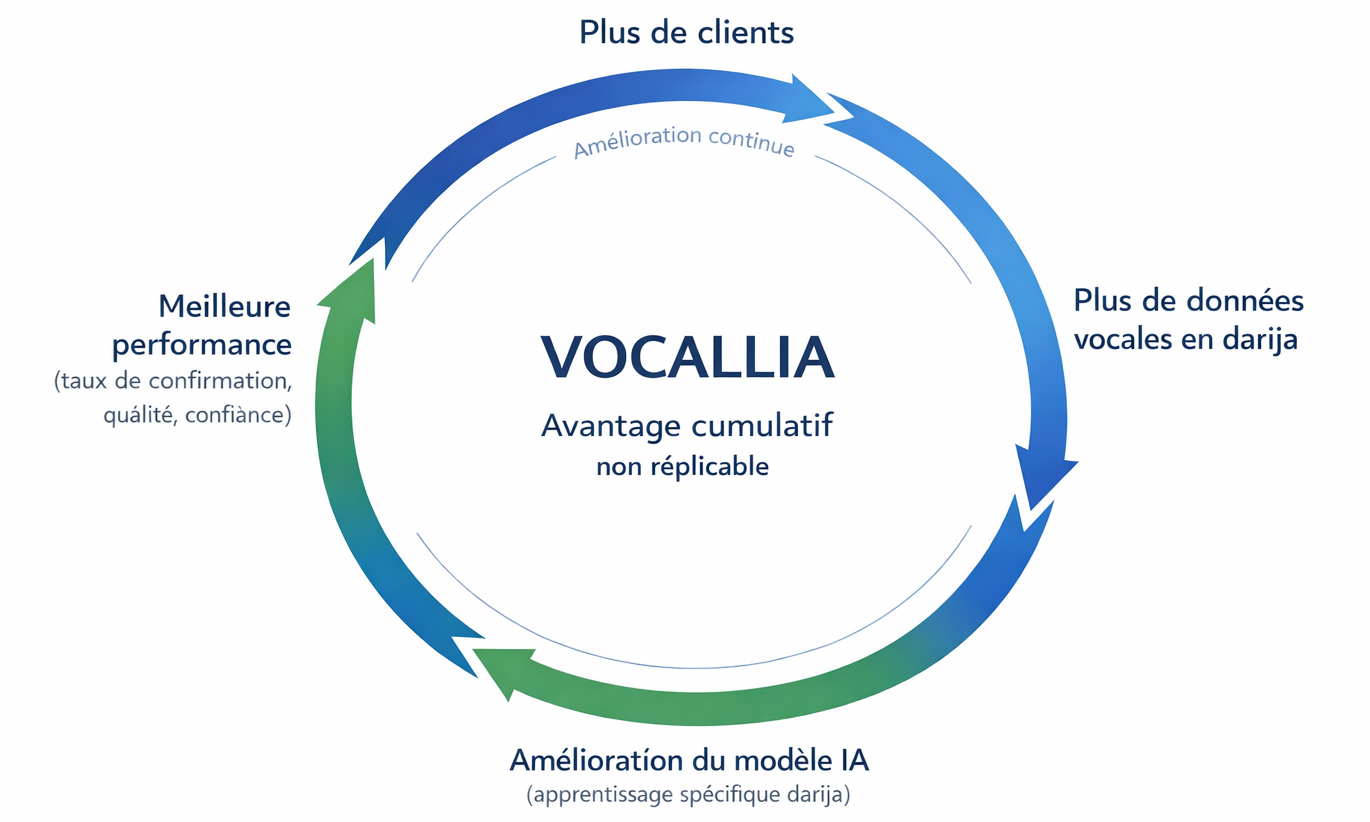
\includegraphics[width=0.68\textwidth]{figures/flywheel-vocallia.png}
    \caption{Mécanisme de \emph{flywheel} --- L'avantage concurrentiel auto-renforçant de Vocallia}
    \label{fig:flywheel-vocallia}
\end{figure}

\begin{tcolorbox}[colback=gray!8, colframe=gray!50, title=\textbf{Fossé concurrentiel de Vocallia --- Architecture du \emph{Moat}}, fonttitle=\bfseries]
Le fossé concurrentiel de Vocallia repose sur quatre piliers complémentaires et auto-renforçants, qui ensemble forment une position défendable sur un horizon de 3 à 5~ans.

La \textbf{barrière linguistique} constitue l'avantage immédiat~: le dialecte tunisien, non standardisé, à code-switching arabe/français dense, est une langue que les modèles globaux ne maîtrisent pas sans données locales. Cette maîtrise ne s'achète pas~: elle se construit par accumulation d'exemples réels et d'itérations sur le terrain.

Le \textbf{corpus de données propriétaires} génère un avantage croissant~: chaque appel traité enrichit un corpus exclusif et non reproductible. À 10\,000 appels, l'écart est significatif. À 100\,000 appels, il est infranchissable. Chaque point de précision gagné se traduit directement en livraisons échouées évitées --- et donc en valeur économique mesurable.

Le \textbf{mécanisme de \emph{flywheel}} (figure~\ref{fig:flywheel-vocallia}) produit un avantage exponentiel~: données $\rightarrow$ amélioration du modèle $\rightarrow$ meilleures performances $\rightarrow$ nouveaux clients $\rightarrow$ davantage de données.

Enfin, les \textbf{intégrations locales et \emph{switching costs}} assurent la rétention~: les intégrations avec les workflows tunisiens, combinées à la personnalisation des scripts, créent des coûts de changement significatifs et croissants. Chaque client intégré est un client structurellement fidélisé.

\medskip
\noindent Ensemble, ces quatre piliers positionnent Vocallia comme le seul acteur capable d'adresser simultanément la dimension linguistique, opérationnelle, économique et réglementaire du marché tunisien --- avantage compétitif défendable et auto-renforçant sur un horizon de trois à cinq ans.
\end{tcolorbox}

%%%%%%%%%%%%%%%%%%%%%%%%%%%%%%%%%%%%%%%%%%%%%%%%%%%%%%%%%%%%%%%%%%%%%%%%%%%
\section{Identification et cartographie des parties prenantes}
\label{section2.6}
%%%%%%%%%%%%%%%%%%%%%%%%%%%%%%%%%%%%%%%%%%%%%%%%%%%%%%%%%%%%%%%%%%%%%%%%%%%

La cartographie des parties prenantes identifie les acteurs qui conditionnent le développement de Vocallia, leurs attentes et la nature de leur influence sur la trajectoire du projet.

\begin{table}[H]
\centering
\caption{Cartographie des parties prenantes --- Vocallia}
\smallskip
\begin{tabular}{|p{2.5cm}|p{2cm}|p{4cm}|p{4cm}|}
\hline
\textbf{Partie prenante} & \textbf{Type} & \textbf{Attentes principales} & \textbf{Nature de l'influence} \\
\hline
E-commerçants (B2B) & Client direct & ROI mesurable, intégration fluide, prix accessible & \textbf{Déterminante}~: adoption = validation commerciale et génération de données \\
\hline
Clients finaux (acheteurs) & Utilisateur indirect & Appel naturel, bref, en dialecte local & Forte~: expérience négative = image dégradée pour le marchand partenaire \\
\hline
Providers API (OpenAI, ElevenLabs, Twilio) & Fournisseur & Volume d'appels, respect des CGU & Modérée~: contraintes tarifaires et quotas techniques \\
\hline
INPDP & Régulateur & Conformité loi 2004-63, licéité du traitement vocal & Modérée à élevée~: conditionne l'autorisation opérationnelle \\
\hline
Investisseurs / Startup Act & Financeur & Traction, croissance, équipe, défendabilité du modèle & \textbf{Élevée}~: conditionne le financement et la vitesse d'exécution \\
\hline
Équipe fondatrice & Interne & Vision, ressources, exécution & \textbf{Déterminante}~: la qualité d'exécution est le principal facteur de succès \\
\hline
\end{tabular}
\end{table}

Deux parties prenantes conditionnent la trajectoire à court terme de manière asymétrique. Les e-commerçants clients sont le moteur primaire~: chaque client acquis valide le modèle, génère des données propriétaires et produit un revenu récurrent. L'INPDP constitue le verrou réglementaire~: l'engager proactivement avant le déploiement commercial transforme une contrainte potentielle en signal de crédibilité vis-à-vis des investisseurs et des clients institutionnels. La priorité opérationnelle des six premiers mois est ainsi clairement établie~: acquérir les premiers clients pilotes et obtenir la validation réglementaire --- dans cet ordre de levier, mais en parallèle d'exécution.

%%%%%%%%%%%%%%%%%%%%%%%%%%%%%%%%%%%%%%%%%%%%%%%%%%%%%%%%%%%%%%%%%%%%%%%%%%%
\section{Carte d'empathie --- Profil du client cible}
\label{section2.7}
%%%%%%%%%%%%%%%%%%%%%%%%%%%%%%%%%%%%%%%%%%%%%%%%%%%%%%%%%%%%%%%%%%%%%%%%%%%

La carte d'empathie (Osterwalder \& Pigneur, 2010~; Dave Gray, 2010) permet de dépasser la description fonctionnelle du client pour appréhender sa réalité vécue. Pour Vocallia, le profil cible est le gérant ou responsable opérationnel d'une boutique e-commerce tunisienne traitant 10 à 50 commandes par jour~: un entrepreneur dont la croissance est freinée non par l'absence de demande, mais par une incapacité opérationnelle à traiter le volume d'interactions clients avec les ressources disponibles.

\begin{figure}[H]
    \centering
    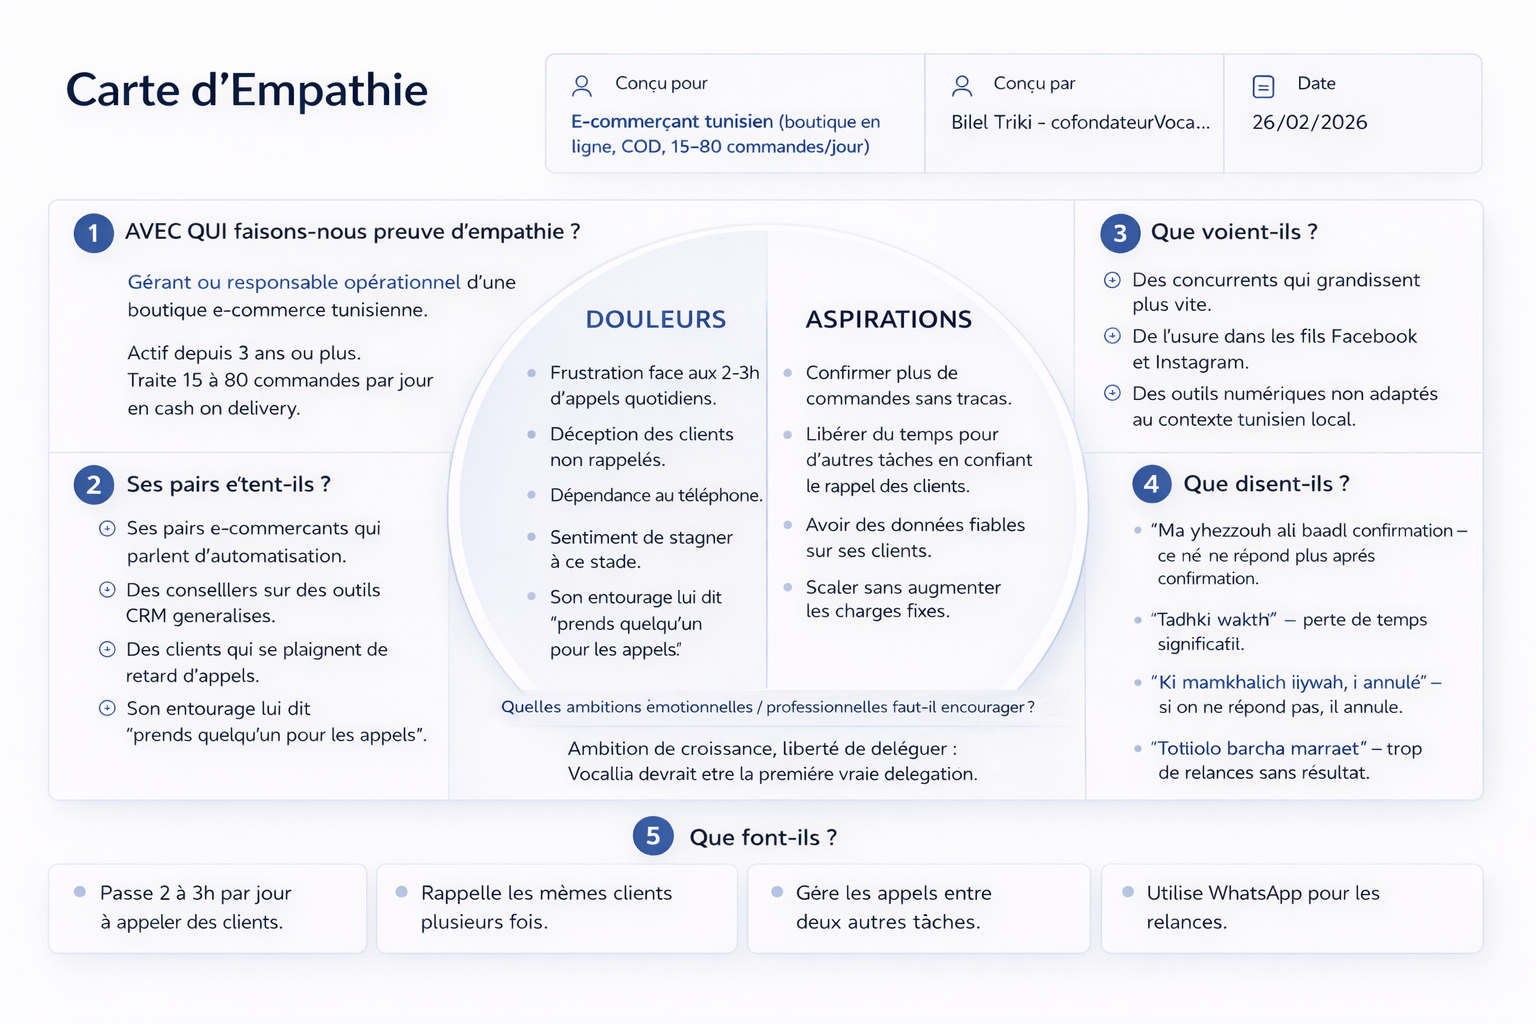
\includegraphics[width=\textwidth]{carte-empathie-vocallia.png}
    \caption{Carte d'empathie --- Profil du client cible Vocallia}
    \label{fig:empathie-vocallia}
\end{figure}

\textit{Source~: Inspiré de Dave Gray, Empathy Map Canvas (2010) --- enrichi des données de l'étude exploratoire Muvaka (collecte avril 2025).}

Ce profil éclaire un impératif stratégique fondamental~: le client cible ne cherche pas une solution d'IA --- il cherche à récupérer du temps, à ne plus perdre de ventes et à sortir du cycle épuisant des appels répétitifs. L'argument de vente de Vocallia n'est pas technologique --- il est économique et humain~: «~Combien de ventes avez-vous perdues ce mois-ci par manque de temps pour rappeler~?~» La réponse à cette question, documentée par les données Muvaka (77,3~\% de marchands concernés), est le meilleur commercial que Vocallia puisse avoir.

%%%%%%%%%%%%%%%%%%%%%%%%%%%%%%%%%%%%%%%%%%%%%%%%%%%%%%%%%%%%%%%%%%%%%%%%%%%
\section{Conclusion}
\label{conclusion2}
%%%%%%%%%%%%%%%%%%%%%%%%%%%%%%%%%%%%%%%%%%%%%%%%%%%%%%%%%%%%%%%%%%%%%%%%%%%

L'analyse de marché conduite dans ce chapitre établit quatre conclusions qui fondent la thèse d'investissement de Vocallia.

\textbf{Le marché est captif.} Avec 84~\% des transactions réglées en \emph{cash on delivery} et une croissance sectorielle de 41,6~\%, la confirmation téléphonique n'est pas un choix --- c'est une obligation opérationnelle dont l'intensité croît avec le volume. Même pour un petit marchand traitant 10 à 15 commandes par jour, le coût cumulé des retours et de la gestion manuelle des appels représente entre 700 et 1\,400~DT par mois (figure~\ref{fig:cout-commande-non-confirmee}) --- charge significative pour une PME aux marges étroites, et suffisante pour justifier le recours à l'automatisation.

\textbf{La demande est validée.} 77,3~\% des marchands interrogés associent le problème à une perte directe de chiffre d'affaires, 85~\% expriment un intérêt fort pour une IA en dialecte tunisien, 90,9~\% acceptent un pilote (figure~\ref{fig:kpi-muvaka}). Signal directionnel suffisant pour déclencher l'exécution.

\textbf{L'espace concurrentiel est vide --- et temporairement.} Aucune solution ne combine voix IA, darija natif, code-switching et pricing PME (figure~\ref{fig:radar-positionnement}). Le fossé de Vocallia --- données propriétaires, \emph{flywheel}, \emph{switching costs} --- se compose avec le temps. Mais il ne se construit que si la position est occupée maintenant.

\textbf{La fenêtre est ouverte --- mais bornée.} IA vocale mature, coûts API décroissants, Startup Act mobilisable, marché vierge. Dans 18 à 36~mois, ces conditions auront changé (figure~\ref{fig:timeline-fenetre}).

\begin{figure}[H]
    \centering
    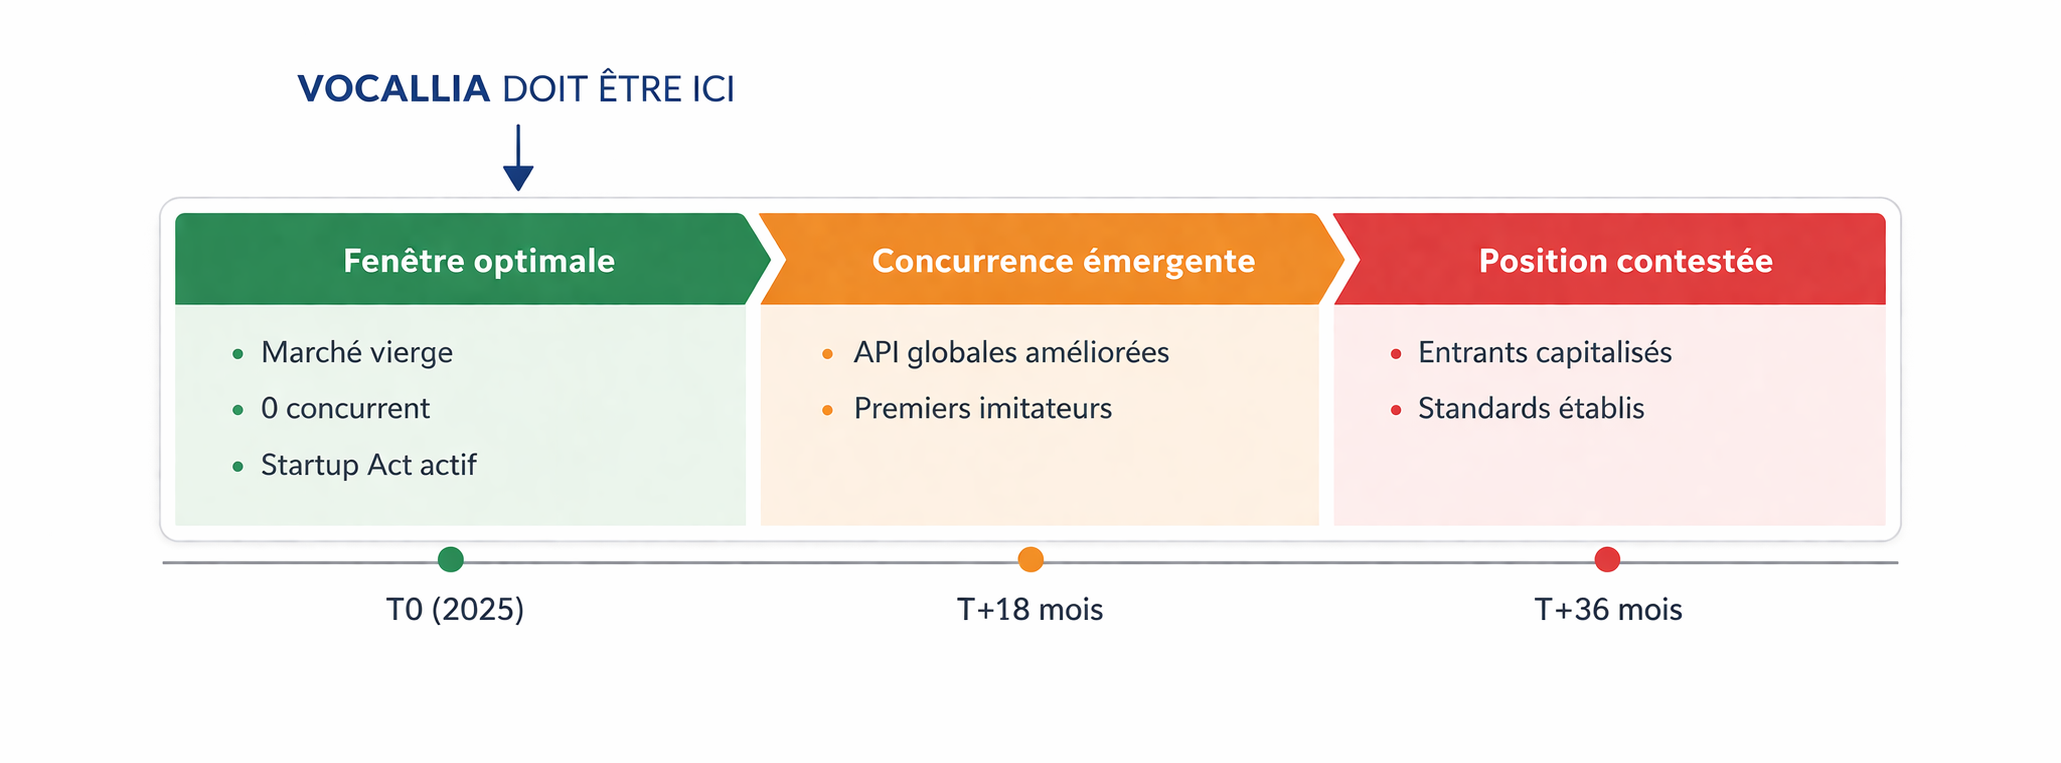
\includegraphics[width=0.95\textwidth]{figures/timeline-fenetre-execution.png}
    \caption{Fenêtre d'exécution de Vocallia --- Urgence temporelle et dynamique concurrentielle}
    \label{fig:timeline-fenetre}
\end{figure}

Vocallia ne se positionne pas comme un outil ponctuel, mais comme la première brique d'une infrastructure conversationnelle en dialecte tunisien --- un actif dont la valeur croît avec chaque interaction, chaque client, chaque verticale. Le marché ne demande pas si cette transition aura lieu~: il demande qui l'opérera en premier.

\begin{tcolorbox}[colback=gray!8, colframe=gray!50, title=\textbf{Thèse d'investissement}, fonttitle=\bfseries]
\begin{center}
\emph{Inefficience non optionnelle. Marché captif en croissance. Espace concurrentiel vide. Fossé défendable qui se renforce par l'usage. La question n'est pas de savoir si le e-commerce tunisien automatisera la confirmation vocale --- mais si Vocallia sera celui qui imposera le standard. La fenêtre est ouverte. Elle ne le restera pas.}
\end{center}
\end{tcolorbox}

\begin{quote}
\textit{Le chapitre suivant traduit ces fondations analytiques en stratégie commerciale opérationnelle~: segmentation, ciblage, proposition de valeur (Value Proposition Canvas), architecture de pricing et modèle économique SaaS --- en mobilisant les outils de la finance entrepreneuriale pour démontrer la viabilité et le potentiel de Vocallia à l'horizon trois ans.}
\end{quote}
%%%%%%%%%%%%%%%%%%%%%%%%%%%%%%%%%%%%%%%%%%%%%%%%%%%%%%%%%%%%%%%%%%%%%%%%%%%
\chapter{Étude de la viabilité commerciale}
\label{Chapitre_3}
%%%%%%%%%%%%%%%%%%%%%%%%%%%%%%%%%%%%%%%%%%%%%%%%%%%%%%%%%%%%%%%%%%%%%%%%%%%

\textit{Démontrer la viabilité commerciale d'une solution ne se limite pas à identifier un besoin ou à décrire un produit : cela exige de prouver que l'offre est monétisable, scalable et défendable dans un contexte concurrentiel donné. Ce chapitre construit la stratégie commerciale de Vocallia selon une chaîne logique unique où chaque décision découle de la précédente et prépare la suivante : la segmentation identifie à qui vendre en premier ; le positionnement formule pourquoi ces clients choisiront Vocallia ; le Value Proposition Canvas vérifie que le produit répond précisément à leurs douleurs ; l'analyse SWOT fixe les priorités d'exécution ; le modèle économique organise la capture de valeur ; le marketing mix et le go-to-market en déploient les leviers opérationnels ; la tarification, les unit economics et les projections financières en démontrent la rentabilité. L'ensemble constitue un plan d'action commercial directement opérationnel, destiné à guider les premières années d'activité de Vocallia.}

%%%%%%%%%%%%%%%%%%%%%%%%%%%%%%%%%%%%%%%%%%%%%%%%%%%%%%%%%%%%%%%%%%%%%%%%%%%
\section{Segmentation et ciblage}
\label{section3.1}
%%%%%%%%%%%%%%%%%%%%%%%%%%%%%%%%%%%%%%%%%%%%%%%%%%%%%%%%%%%%%%%%%%%%%%%%%%%

La segmentation est l'acte fondateur de toute stratégie commerciale : elle détermine à qui l'on s'adresse, dans quel ordre, et avec quels arguments. Pour Vocallia, cette décision est d'autant plus critique que le marché e-commerce tunisien est hétérogène --- il mêle des structures formalisées aux boutiques informelles sur réseaux sociaux, des marchands numériquement matures à ceux qui découvrent les outils digitaux. En phase d'amorçage, se tromper de cible initiale ne ralentit pas la croissance : cela tue le projet. Concentrer les ressources sur le segment où la douleur est la plus aiguë, la capacité à payer la plus immédiate et le cycle de vente le plus court est une condition de survie.

%%%%%%%%%%%%%%%%%%%%%%%%%%%%%%%%%%%%%%%%%%%%%%%%%%%%%%%%%%%%%%%%%%%%%%%%%%%
\subsection{Segmentation multicritères}
\label{section3.1.1}
%%%%%%%%%%%%%%%%%%%%%%%%%%%%%%%%%%%%%%%%%%%%%%%%%%%%%%%%%%%%%%%%%%%%%%%%%%%

La segmentation de Vocallia repose sur une approche multicritères combinant des dimensions opérationnelles, comportementales et économiques. Elle s'appuie sur les données collectées lors de l'étude exploratoire terrain (22 répondants, avril 2025) et sur l'analyse du marché e-commerce tunisien (BCT, 2024). Six critères structurants ont été retenus, chacun constituant un filtre discriminant pour évaluer l'intensité du besoin, la capacité d'adoption et la solvabilité de chaque segment.

\begin{table}[H]
\centering
\caption{Segmentation multicritères --- Vocallia (2025)}
\vspace{4pt}
\begin{tabularx}{\textwidth}{|>{\raggedright\arraybackslash}p{3cm}|>{\raggedright\arraybackslash}X|>{\raggedright\arraybackslash}X|>{\raggedright\arraybackslash}X|}
\hline
\textbf{Critère} & \textbf{Segment A \newline Cible prioritaire} & \textbf{Segment B \newline Cible secondaire} & \textbf{Segment C \newline Hors cible initiale} \\
\hline
Volume commandes/jour & $>$ 15 commandes & 6 à 15 commandes & $<$ 5 commandes \\
\hline
Mode de paiement dominant & Cash on delivery (COD) exclusif & COD et prépaiement mixte & Prépaiement majoritaire \\
\hline
Ancienneté de la boutique & 3 ans et plus & 1 à 3 ans & Moins de 1 an \\
\hline
Gestion des appels & Gérant ou employé dédié & Gérant seul, sans ressource & Externalisé ou inexistant \\
\hline
Appétence digitale & Utilise déjà des outils SaaS & Utilisateur partiel, curieux & Faible maturité digitale \\
\hline
Budget mensuel estimé & 100--300 DT/mois & 50--100 DT/mois & $<$ 50 DT/mois \\
\hline
Intensité du besoin & \textbf{Critique} --- le problème est coûteux et quotidien & \textbf{Réelle} --- le problème est présent mais supportable & \textbf{Faible} --- pas de friction opérationnelle identifiée \\
\hline
Priorité commerciale & \textbf{Haute} & Moyenne & \textbf{Absente au lancement} \\
\hline
\end{tabularx}
\end{table}

La matrice de priorisation (figure~\ref{fig:matrice_segments}) synthétise visuellement cette hiérarchisation en croisant l'intensité du besoin avec la capacité à payer de chaque segment.

\begin{figure}[H]
\centering
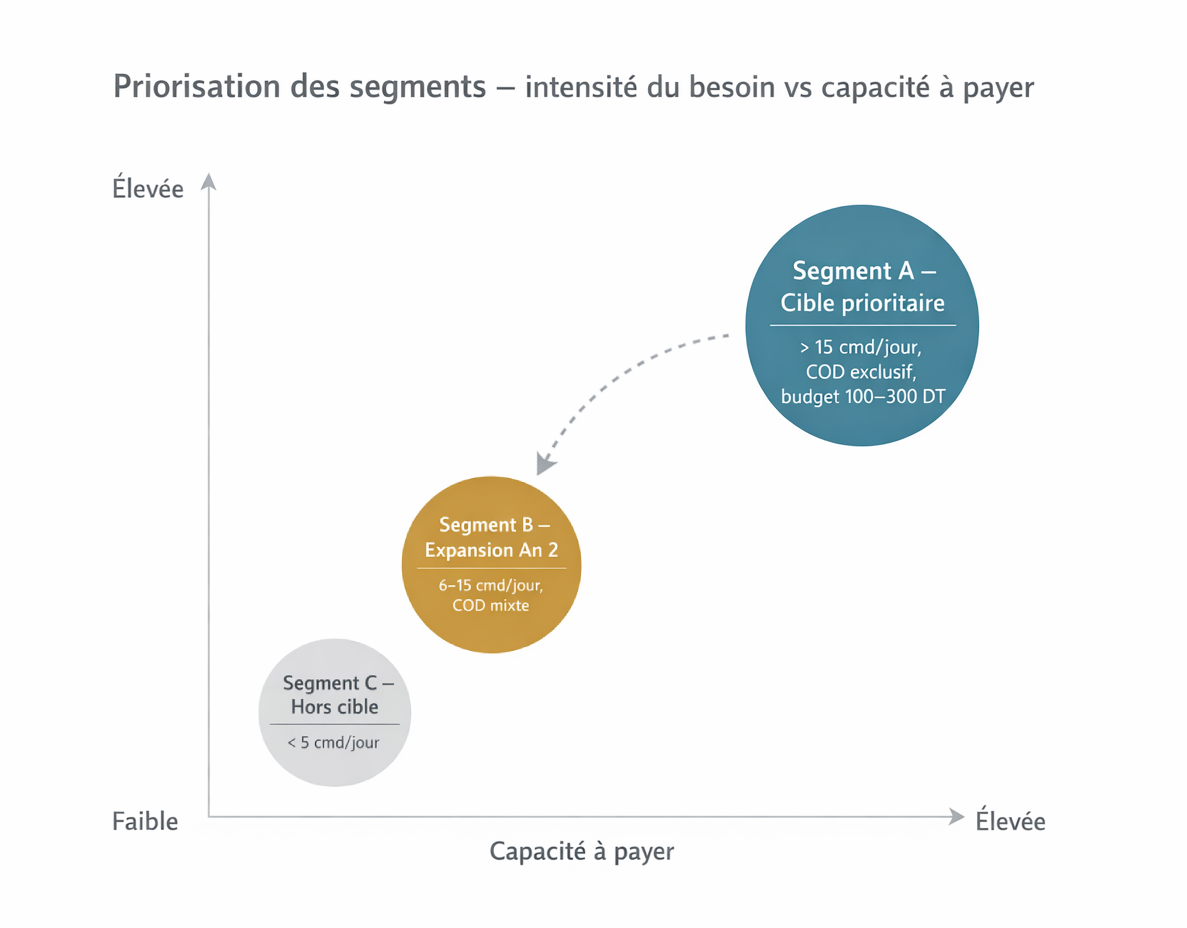
\includegraphics[width=0.82\textwidth]{figures/matrice_priorisation_segments.png}
\caption{Priorisation des segments --- intensité du besoin vs capacité à payer}
\label{fig:matrice_segments}
\end{figure}

\noindent\textbf{Lecture stratégique de la segmentation.} Le Segment A est le seul où Vocallia génère de la valeur dès le premier mois, avec un risque commercial minimal et un cycle de vente court. Le Segment B représente un réservoir de croissance naturel à moyen terme : ces marchands basculeront lorsque les résultats du Segment A fourniront les preuves sociales nécessaires. Le Segment C est délibérément exclu au lancement : le coût d'acquisition y serait disproportionné, le risque de churn élevé, et l'impact sur les métriques SaaS destructeur dans une phase où chaque point de crédibilité compte.

Cette hiérarchisation conditionne l'intégralité de la stratégie qui suit : le positionnement sera formulé pour le Segment A, la proposition de valeur calibrée sur ses douleurs, le pricing ancré dans sa zone de confort budgétaire, et le go-to-market optimisé pour son cycle de décision.

%%%%%%%%%%%%%%%%%%%%%%%%%%%%%%%%%%%%%%%%%%%%%%%%%%%%%%%%%%%%%%%%%%%%%%%%%%%
\subsection{Personas commerciaux}
\label{section3.1.2}
%%%%%%%%%%%%%%%%%%%%%%%%%%%%%%%%%%%%%%%%%%%%%%%%%%%%%%%%%%%%%%%%%%%%%%%%%%%

Au-delà des segments, la stratégie commerciale est orientée par deux personas représentatifs, construits à partir des données qualitatives de l'étude terrain. Ces profils ne sont pas des archétypes théoriques : ils incarnent des réalités opérationnelles documentées, et servent de guide aussi bien pour la conception produit que pour les argumentaires de vente.

\begin{figure}[H]
\centering
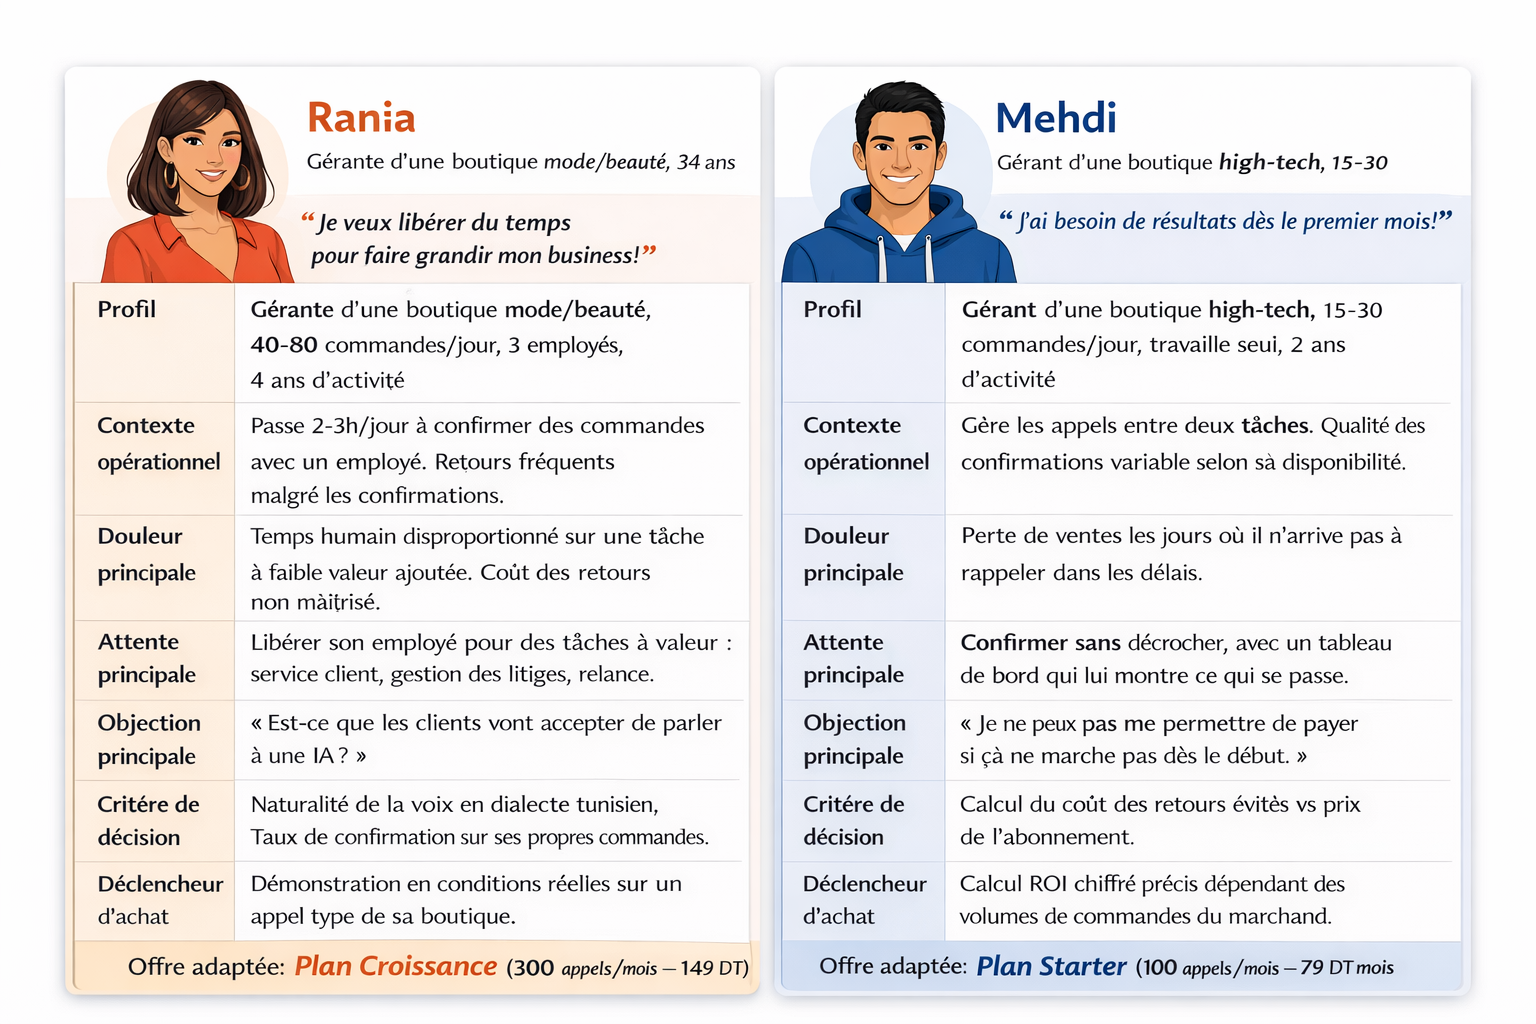
\includegraphics[width=\textwidth]{figures/personas_vocallia.png}
\caption{Personas commerciaux --- Vocallia}
\label{fig:personas}
\end{figure}

\noindent\textbf{Interprétation stratégique des personas.} Les deux profils structurent des approches commerciales distinctes, mais convergent vers un même impératif : la preuve par le résultat. Avec Rania, le levier de conversion est la libération de capacité opérationnelle et la réduction mesurable des coûts --- un argument qui se traduit directement en économies chiffrées sur le dashboard. Avec Mehdi, le levier est la tranquillité opérationnelle et la rapidité du gain perçu, condition non négociable pour déclencher l'achat chez un dirigeant qui investit sur ses fonds propres. Dans les deux cas, le moment de bascule du cycle de vente est le même : l'écoute d'un appel réel en dialecte tunisien, validé comme le déclencheur de conversion le plus puissant lors de la phase Muvaka. Ce constat oriente directement le positionnement : Vocallia doit se vendre comme une performance opérationnelle audible et mesurable, pas comme une promesse technologique.

%%%%%%%%%%%%%%%%%%%%%%%%%%%%%%%%%%%%%%%%%%%%%%%%%%%%%%%%%%%%%%%%%%%%%%%%%%%
\section{Positionnement stratégique}
\label{section3.2}
%%%%%%%%%%%%%%%%%%%%%%%%%%%%%%%%%%%%%%%%%%%%%%%%%%%%%%%%%%%%%%%%%%%%%%%%%%%

Le positionnement est la décision stratégique la plus structurante du plan commercial : il détermine comment la marque veut être perçue, par rapport à qui, et sur quelle promesse irréductible. La segmentation a identifié le Segment A comme cible prioritaire ; les personas ont révélé que le critère de décision est la performance opérationnelle mesurable, pas l'innovation technologique. Le positionnement de Vocallia en découle directement. Dans un marché où aucun concurrent local direct n'existe encore, ce positionnement n'est pas défensif --- il est fondateur. L'enjeu n'est pas de se différencier d'un concurrent, mais de définir la catégorie avant que quiconque ne tente de l'occuper.

\medskip
\noindent\textbf{Énoncé de positionnement.} \textit{Vocallia est la première infrastructure locale d'automatisation vocale intelligente pour les e-commerçants tunisiens : elle confirme vos commandes en dialecte tunisien, 24h/24, à un coût marginal faible, avec une traçabilité complète --- pour que vous confirmiez plus, perdiez moins, et vous concentriez sur ce qui fait vraiment croître votre activité.}

\medskip
Ce positionnement repose sur trois piliers stratégiques distincts et défendables à moyen terme (figure~\ref{fig:positionnement_piliers}).

\begin{figure}[H]
\centering
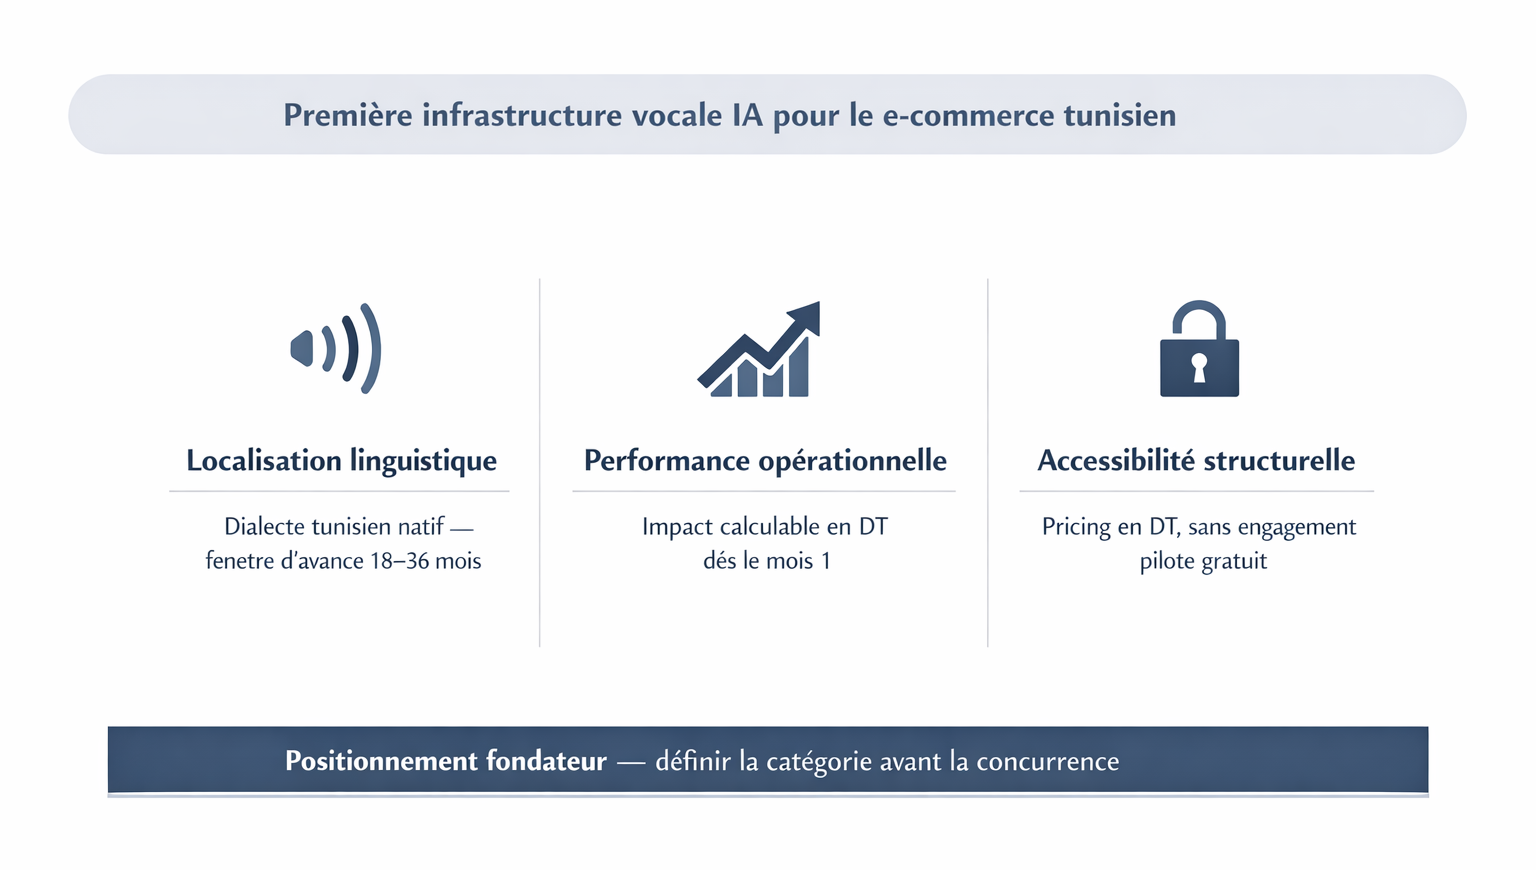
\includegraphics[width=\textwidth]{figures/positionnement_3piliers.png}
\caption{Positionnement stratégique Vocallia --- trois piliers défendables}
\label{fig:positionnement_piliers}
\end{figure}

La \textbf{localisation linguistique} --- maîtrise du dialecte tunisien (darija) et du code-switching arabe/français --- constitue une barrière à l'entrée que les acteurs globaux (Bland.ai, Vapi.ai, Retell AI) ne peuvent franchir sans un investissement local spécifique, coûteux et long. Cette barrière offre une fenêtre d'avance de 18 à 36 mois, suffisante pour construire une base de clients, un corpus de données d'appels locales et une réputation terrain irremplaçables.

L'\textbf{orientation performance opérationnelle} positionne Vocallia non comme une technologie, mais comme un levier de performance dont l'impact est calculable en dinars dès le premier mois d'usage. Cette posture --- partenaire de croissance plutôt que fournisseur technologique --- est décisive pour des PME dont le budget est contraint et dont la patience pour un outil sans résultat visible est nulle.

L'\textbf{accessibilité structurelle} --- pricing en dinars tunisiens, sans engagement long terme, avec un pilote gratuit --- élimine les trois principaux freins à l'adoption identifiés sur le terrain : le risque financier, la méfiance envers un outil nouveau, et l'absence de référence locale. Ces éléments ne sont pas des concessions --- ils font partie intégrante de la promesse de marque et structurent le modèle d'acquisition décrit dans les sections suivantes.

\medskip
Ce positionnement à trois piliers formule une promesse. La section suivante vérifie, à travers le Value Proposition Canvas, que cette promesse est effectivement tenue par le produit : chaque pilier doit correspondre à une douleur documentée, et chaque fonctionnalité doit y répondre avec précision.

%%%%%%%%%%%%%%%%%%%%%%%%%%%%%%%%%%%%%%%%%%%%%%%%%%%%%%%%%%%%%%%%%%%%%%%%%%%
\section{Proposition de valeur --- Value Proposition Canvas}
\label{section3.3}
%%%%%%%%%%%%%%%%%%%%%%%%%%%%%%%%%%%%%%%%%%%%%%%%%%%%%%%%%%%%%%%%%%%%%%%%%%%

Le Value Proposition Canvas (Osterwalder, Pigneur, Bernarda \& Smith, 2014) met en correspondance explicite le profil du client avec la carte de valeur du produit. Il sert ici de test de cohérence : le positionnement promet localisation, performance et accessibilité --- le VPC vérifie que le produit délivre sur ces trois axes. Toute fonctionnalité sans douleur correspondante serait superflue ; toute promesse sans ancrage terrain serait un risque commercial.

%%%%%%%%%%%%%%%%%%%%%%%%%%%%%%%%%%%%%%%%%%%%%%%%%%%%%%%%%%%%%%%%%%%%%%%%%%%
\subsection{Profil client}
\label{section3.3.1}
%%%%%%%%%%%%%%%%%%%%%%%%%%%%%%%%%%%%%%%%%%%%%%%%%%%%%%%%%%%%%%%%%%%%%%%%%%%

\begin{table}[H]
\centering
\caption{Profil client --- Value Proposition Canvas Vocallia}
\vspace{4pt}
\begin{tabularx}{\textwidth}{|>{\raggedright\arraybackslash}p{2.5cm}|>{\raggedright\arraybackslash}X|>{\raggedright\arraybackslash}X|}
\hline
\textbf{Dimension} & \textbf{Description détaillée} & \textbf{Preuve terrain} \\
\hline
\textbf{Jobs à accomplir} & Confirmer les commandes avant expédition. Gérer les demandes d'information client (délai, suivi). Maintenir la relation client pendant la livraison. Piloter le taux de retour. & Structurel : 84~\% des transactions en COD (BCT, 2024). Besoin quotidien, non délégable sans risque. \\
\hline
\textbf{Douleurs (Pains)} & Temps excessif mobilisé sur des appels répétitifs à faible valeur. Clients injoignables générant des retours coûteux. Annulations post-confirmation non anticipées. Qualité variable des échanges humains. Absence totale de données sur les raisons d'annulation. & 77,3~\% ont perdu des opportunités de vente (étude terrain, avr. 2025). Coût logistique d'un retour estimé à 12 DT (transport aller-retour). \\
\hline
\textbf{Gains attendus (Gains)} & Augmenter le taux de confirmation sans recruter. Libérer du temps pour des tâches à valeur. Réduire le taux de retour. Disposer d'un tableau de bord sur les annulations. Scaler l'activité sans augmenter les coûts fixes. & 90,9~\% se déclarent prêts à tester un pilote (étude terrain, avr. 2025). \\
\hline
\end{tabularx}
\end{table}

%%%%%%%%%%%%%%%%%%%%%%%%%%%%%%%%%%%%%%%%%%%%%%%%%%%%%%%%%%%%%%%%%%%%%%%%%%%
\subsection{Carte de valeur Vocallia}
\label{section3.3.2}
%%%%%%%%%%%%%%%%%%%%%%%%%%%%%%%%%%%%%%%%%%%%%%%%%%%%%%%%%%%%%%%%%%%%%%%%%%%

\begin{table}[H]
\centering
\caption{Carte de valeur --- Value Proposition Canvas Vocallia}
\vspace{4pt}
\begin{tabularx}{\textwidth}{|>{\raggedright\arraybackslash}p{2.5cm}|>{\raggedright\arraybackslash}X|>{\raggedright\arraybackslash}X|}
\hline
\textbf{Dimension} & \textbf{Réponse Vocallia} & \textbf{Alignement avec le profil client} \\
\hline
\textbf{Produits et services} & Agent vocal IA sortant, dialecte tunisien natif, disponible 24h/24, tableau de bord temps réel, transcriptions d'appels, intégration CRM via webhook, fallback humain automatique. & Couvre l'intégralité des Jobs identifiés sans intervention humaine constante. \\
\hline
\textbf{Analgésiques (Pain relievers)} & Appels automatiques $\rightarrow$ temps libéré. Script standardisé $\rightarrow$ qualité constante. Détection d'annulation $\rightarrow$ alerte immédiate. Fallback humain $\rightarrow$ aucun blocage conversationnel. Consentement vocal $\rightarrow$ conformité INPDP. & Adresse directement et précisément les 5 douleurs documentées sur le terrain. \\
\hline
\textbf{Créateurs de gains (Gain creators)} & Plus de commandes confirmées $=$ plus de CA. Réduction du taux de retour $=$ économies logistiques mesurables. Données sur les raisons d'annulation $=$ pilotage commercial. Scalabilité sans recrutement $=$ levier de croissance. & Répond aux 4 gains prioritaires exprimés par les personas Rania et Mehdi. \\
\hline
\end{tabularx}
\end{table}

%%%%%%%%%%%%%%%%%%%%%%%%%%%%%%%%%%%%%%%%%%%%%%%%%%%%%%%%%%%%%%%%%%%%%%%%%%%
\subsection{Représentation visuelle du Value Proposition Canvas}
\label{section3.3.3}
%%%%%%%%%%%%%%%%%%%%%%%%%%%%%%%%%%%%%%%%%%%%%%%%%%%%%%%%%%%%%%%%%%%%%%%%%%%

\begin{figure}[H]
\centering
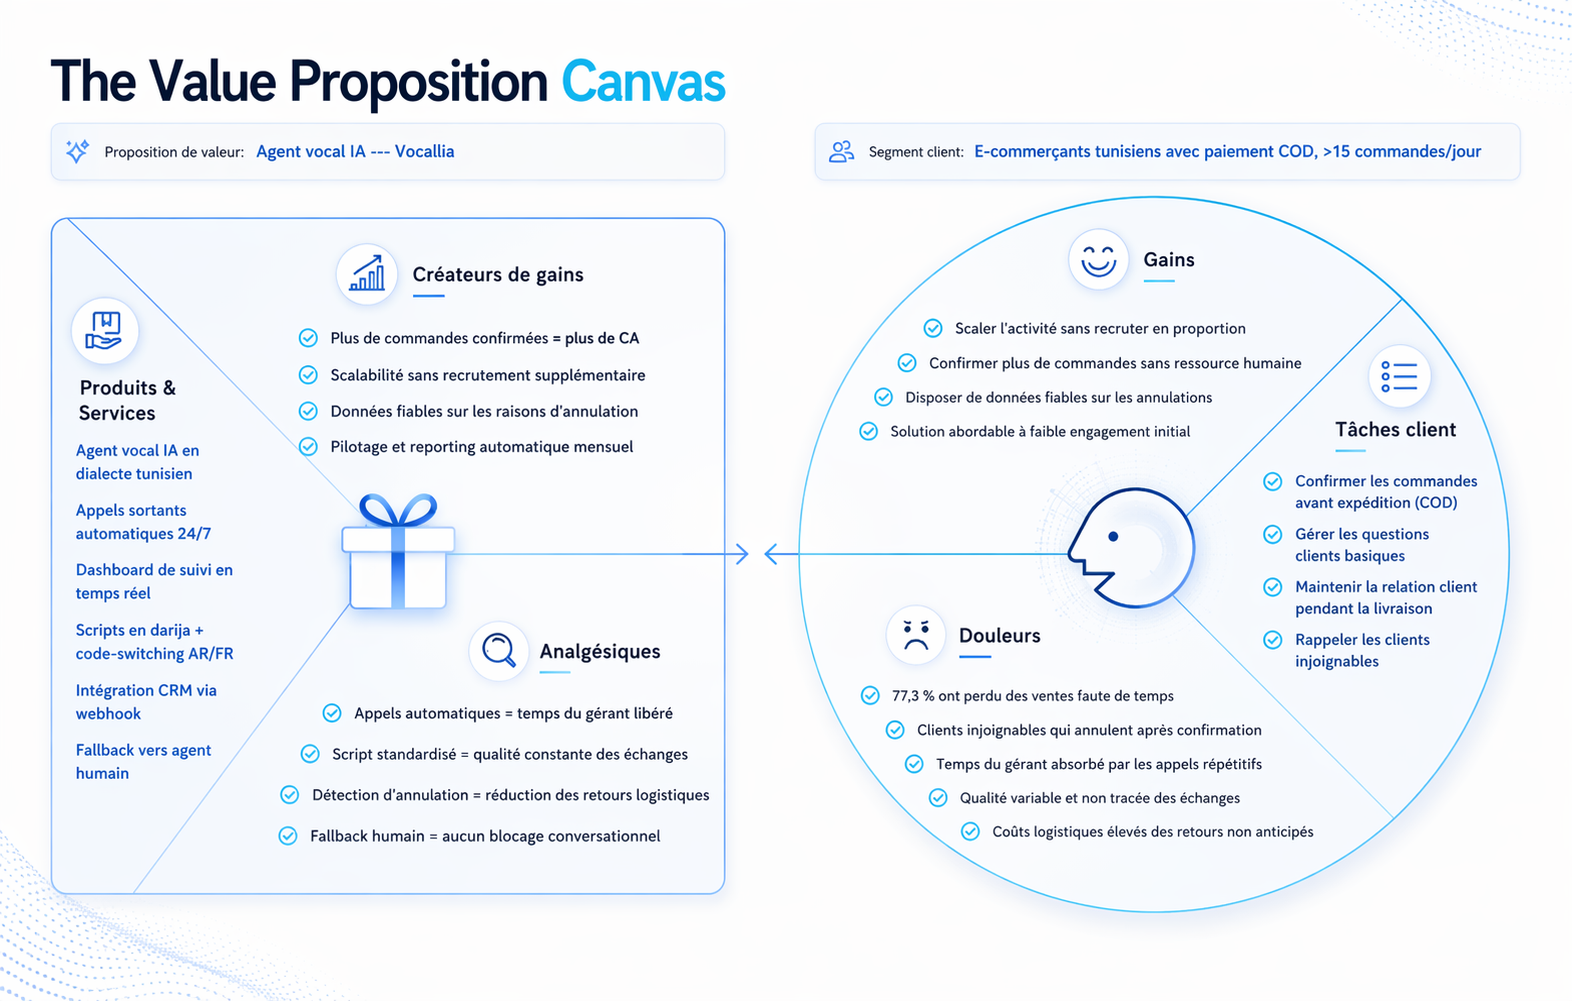
\includegraphics[width=\textwidth]{figures/value_proposition_canvas.png}
\caption{Value Proposition Canvas --- Vocallia (2025)}
\label{fig:vpc}
\end{figure}


\begin{tcolorbox}[colback=gray!8, colframe=gray!50, title=\textbf{Cohérence de la proposition de valeur}, fonttitle=\bfseries]
L'adéquation entre le profil client et la carte de valeur est forte et vérifiable sur les trois dimensions. Le problème opérationnel (confirmation en COD) est direct, quotidien et mesurable en coût. Chaque douleur documentée trouve une réponse fonctionnelle précise dans le produit. Les gains attendus sont quantifiables : commandes confirmées, taux de retour, capacité opérationnelle libérée. Cette triple cohérence --- besoin structurel, réponse précise, valeur mesurable --- valide le positionnement formulé en section~\ref{section3.2} et réduit significativement le risque d'exécution commerciale. Lorsqu'une offre est alignée sur une douleur quotidienne et coûteuse, la vente ne repose pas sur la persuasion mais sur la démonstration --- ce qui change fondamentalement l'économie d'acquisition et la prédictibilité de la conversion.
\end{tcolorbox}

%%%%%%%%%%%%%%%%%%%%%%%%%%%%%%%%%%%%%%%%%%%%%%%%%%%%%%%%%%%%%%%%%%%%%%%%%%%
\section{Analyse SWOT}
\label{section3.4}
%%%%%%%%%%%%%%%%%%%%%%%%%%%%%%%%%%%%%%%%%%%%%%%%%%%%%%%%%%%%%%%%%%%%%%%%%%%

La proposition de valeur étant validée, la question suivante est : dans quelles conditions sera-t-elle déployée~? L'analyse SWOT fournit la réponse en identifiant les forces à exploiter immédiatement, les vulnérabilités à compenser, et les fenêtres d'opportunité à saisir avant qu'elles ne se referment.

\begin{table}[H]
\centering
\caption{Analyse SWOT --- Vocallia (2025)}
\vspace{4pt}
\begin{tabularx}{\textwidth}{|>{\raggedright\arraybackslash}X|>{\raggedright\arraybackslash}X|}
\hline
\textbf{FORCES (internes)} & \textbf{FAIBLESSES (internes)} \\
\hline
\begin{itemize}[leftmargin=*, noitemsep, topsep=3pt, parsep=0pt]
  \item Premier entrant sur un segment non contesté
  \item Maîtrise native du dialecte tunisien et du code-switching AR/FR
  \item Validation terrain documentée : 90,9~\% prêts à tester
  \item Modèle SaaS à marge brute structurellement élevée ($>$70~\%)
  \item Architecture multi-fournisseurs résiliente et substituable
  \item Conformité INPDP intégrée dès la conception
  \item Coût d'acquisition très faible validé (0,36~\euro{}/lead, phase Muvaka)
\end{itemize}
&
\begin{itemize}[leftmargin=*, noitemsep, topsep=3pt, parsep=0pt]
  \item Notoriété et réputation nulles au lancement
  \item Dépendance structurelle aux APIs tierces (OpenAI, Twilio, ElevenLabs)
  \item Équipe réduite : exécution commerciale et technique simultanées difficiles
  \item Aucune référence client publiée au démarrage
  \item Risque de latence et de qualité dialectale sur certains sous-registres
  \item Absence de force de vente dédiée en phase initiale
\end{itemize} \\
\hline
\textbf{OPPORTUNITÉS (externes)} & \textbf{MENACES (externes)} \\
\hline
\begin{itemize}[leftmargin=*, noitemsep, topsep=3pt, parsep=0pt]
  \item Marché local quasi-vierge, aucun concurrent direct identifié
  \item Croissance e-commerce tunisien : $+$41,6~\%/an (BCT, 2023)
  \item 84~\% de transactions en COD $=$ besoin structurel et durable
  \item Startup Act : subventions, exonérations, accès devises
  \item CAGR Voice AI mondial de 34,8~\% (Market.us, 2024)
  \item Démocratisation des APIs LLM $\rightarrow$ réduction continue des coûts variables
  \item Réseau d'e-commerçants tunisiens dense et interconnecté (effet bouche-à-oreille)
\end{itemize}
&
\begin{itemize}[leftmargin=*, noitemsep, topsep=3pt, parsep=0pt]
  \item Désintermédiation si OpenAI améliore radicalement le support de l'arabe dialectal
  \item Entrée de concurrents internationaux mieux capitalisés à moyen terme
  \item Résistance culturelle au remplacement de l'appel humain
  \item Churn élevé si la valeur n'est pas démontrée dans les 30 premiers jours
  \item Évolution réglementaire INPDP sur les données vocales
  \item Dépendance à la stabilité tarifaire des fournisseurs d'API
\end{itemize} \\
\hline
\end{tabularx}
\end{table}


\medskip
\noindent\textbf{Lecture stratégique.} L'analyse SWOT impose quatre priorités d'action immédiates. Premièrement, \textbf{capitaliser sur la fenêtre de premier entrant} : la force linguistique n'est défendable que si Vocallia accumule rapidement des clients actifs, un corpus de données d'appels locales et une réputation terrain avant que les acteurs globaux ne comblent le gap dialectal. La fenêtre est estimée à 18--36 mois --- chaque mois sans client actif est un mois de protection gaspillé. Deuxièmement, \textbf{transformer l'absence de références en levier} en recrutant dès le lancement 3 à 5 marchands pilotes du Segment A disposés à témoigner publiquement : la faiblesse principale devient ainsi un accélérateur d'acquisition. Troisièmement, \textbf{neutraliser le risque de dépendance aux APIs} par l'architecture multi-fournisseurs déjà intégrée dans la conception technique. Quatrièmement, \textbf{faire des 90 premiers jours le moment de vérité} : des résultats mesurables dans ce délai sont le seul rempart efficace simultanément contre le churn et la résistance culturelle.

Ces quatre priorités convergent vers un même impératif d'exécution : accumuler rapidement des résultats clients exploitables commercialement. Le modèle économique doit en être le véhicule --- permettre une entrée sans risque pour le client tout en préservant la marge et la scalabilité pour Vocallia.

%%%%%%%%%%%%%%%%%%%%%%%%%%%%%%%%%%%%%%%%%%%%%%%%%%%%%%%%%%%%%%%%%%%%%%%%%%%
\section{Modèle économique}
\label{section3.5}
%%%%%%%%%%%%%%%%%%%%%%%%%%%%%%%%%%%%%%%%%%%%%%%%%%%%%%%%%%%%%%%%%%%%%%%%%%%

Le modèle économique traduit la proposition de valeur en mécanisme de capture de revenus. Il articule trois logiques : comment le produit crée de la valeur, comment cette valeur atteint le client, et comment Vocallia en monétise une part de façon durable et scalable. Les contraintes sont claires : l'analyse SWOT impose une entrée sans risque pour le client ; la structure de coûts doit rester dominée par les variables pour protéger la marge à toute échelle. Le modèle retenu est hybride : abonnement récurrent (subscription) et facturation à l'usage (usage-based pricing).

%%%%%%%%%%%%%%%%%%%%%%%%%%%%%%%%%%%%%%%%%%%%%%%%%%%%%%%%%%%%%%%%%%%%%%%%%%%
\subsection{Structure des revenus}
\label{section3.5.1}
%%%%%%%%%%%%%%%%%%%%%%%%%%%%%%%%%%%%%%%%%%%%%%%%%%%%%%%%%%%%%%%%%%%%%%%%%%%

\begin{table}[H]
\centering
\caption{Structure des revenus --- Vocallia}
\vspace{4pt}
\begin{tabularx}{\textwidth}{|>{\raggedright\arraybackslash}p{2.5cm}|>{\raggedright\arraybackslash}X|>{\raggedright\arraybackslash}X|>{\raggedright\arraybackslash}p{1.8cm}|}
\hline
\textbf{Source} & \textbf{Description} & \textbf{Logique stratégique} & \textbf{Horizon} \\
\hline
Abonnement mensuel SaaS & Forfait incluant un volume d'appels (Starter / Croissance / Pro) & Revenus récurrents prévisibles. Base du MRR. & Lancement \\
\hline
Facturation à l'usage & Appels supplémentaires au-delà du forfait, à un coût unitaire dégressif & Aligne le coût sur la valeur créée. Réduit la friction à l'entrée. & Lancement \\
\hline
Setup fee / onboarding & Frais uniques de configuration, personnalisation des scripts et intégration CRM pour les comptes Pro & Couvre les coûts d'onboarding. Filtre les clients peu engagés. & Mois 3+ \\
\hline
\end{tabularx}
\end{table}

Ce modèle hybride est particulièrement adapté au contexte tunisien pour trois raisons convergentes. D'abord, il permet une entrée à faible risque financier pour le client (pilote gratuit, puis abonnement mensuel sans engagement), réduisant la résistance initiale à l'adoption --- un impératif identifié par la SWOT. Ensuite, la composante usage crée un alignement naturel entre la valeur perçue et le coût payé : un marchand qui confirme davantage de commandes paie proportionnellement plus, mais génère aussi davantage de revenus. Enfin, la prévisibilité du MRR offre à Vocallia la visibilité financière indispensable pour piloter sa trésorerie en phase d'amorçage sans recourir à un financement externe immédiat.

%%%%%%%%%%%%%%%%%%%%%%%%%%%%%%%%%%%%%%%%%%%%%%%%%%%%%%%%%%%%%%%%%%%%%%%%%%%
\subsection{Structure des coûts}
\label{section3.5.2}
%%%%%%%%%%%%%%%%%%%%%%%%%%%%%%%%%%%%%%%%%%%%%%%%%%%%%%%%%%%%%%%%%%%%%%%%%%%

Le coût variable d'un appel de 2 minutes est de 0,21 DT, réparti entre quatre composantes technologiques (figure~\ref{fig:cout_appel}). Les coûts fixes comprennent l'infrastructure cloud, les outils de développement et d'administration. Les coûts commerciaux couvrent l'acquisition (Meta Ads, SEO) et le support client. La dominance des coûts variables dans cette structure est un avantage structurel : elle protège la marge en phase de faible volume et préserve la scalabilité en phase de croissance.

\begin{figure}[H]
\centering
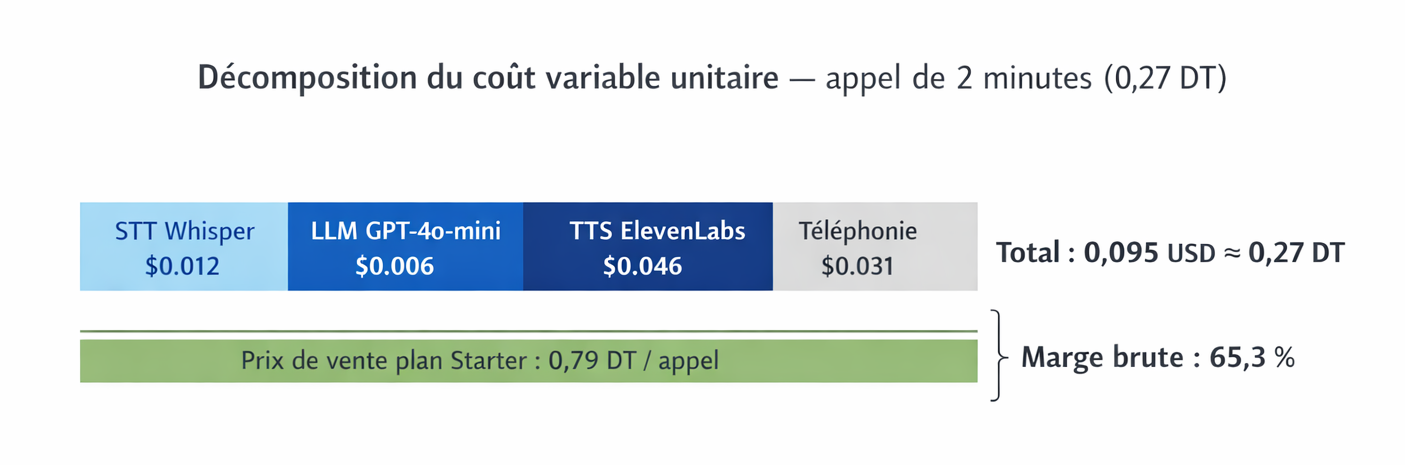
\includegraphics[width=0.92\textwidth]{figures/cout_variable_appel.png}
\caption{Décomposition du coût variable unitaire --- appel de 2 minutes (0,21 DT)}
\label{fig:cout_appel}
\end{figure}

%%%%%%%%%%%%%%%%%%%%%%%%%%%%%%%%%%%%%%%%%%%%%%%%%%%%%%%%%%%%%%%%%%%%%%%%%%%
\subsection{Business Model Canvas}
\label{section3.5.3}
%%%%%%%%%%%%%%%%%%%%%%%%%%%%%%%%%%%%%%%%%%%%%%%%%%%%%%%%%%%%%%%%%%%%%%%%%%%

Le Business Model Canvas (Osterwalder \& Pigneur, 2010) synthétise en une vue l'ensemble des décisions prises dans les sections précédentes --- segments, proposition de valeur, canaux, architecture de revenus --- et les confronte aux ressources, activités et partenariats nécessaires à l'exécution. L'enjeu n'est pas de remplir neuf cases, mais de vérifier que le modèle tient debout quand tous ses blocs sont mis en tension simultanément.

\begin{figure}[H]
    \centering
    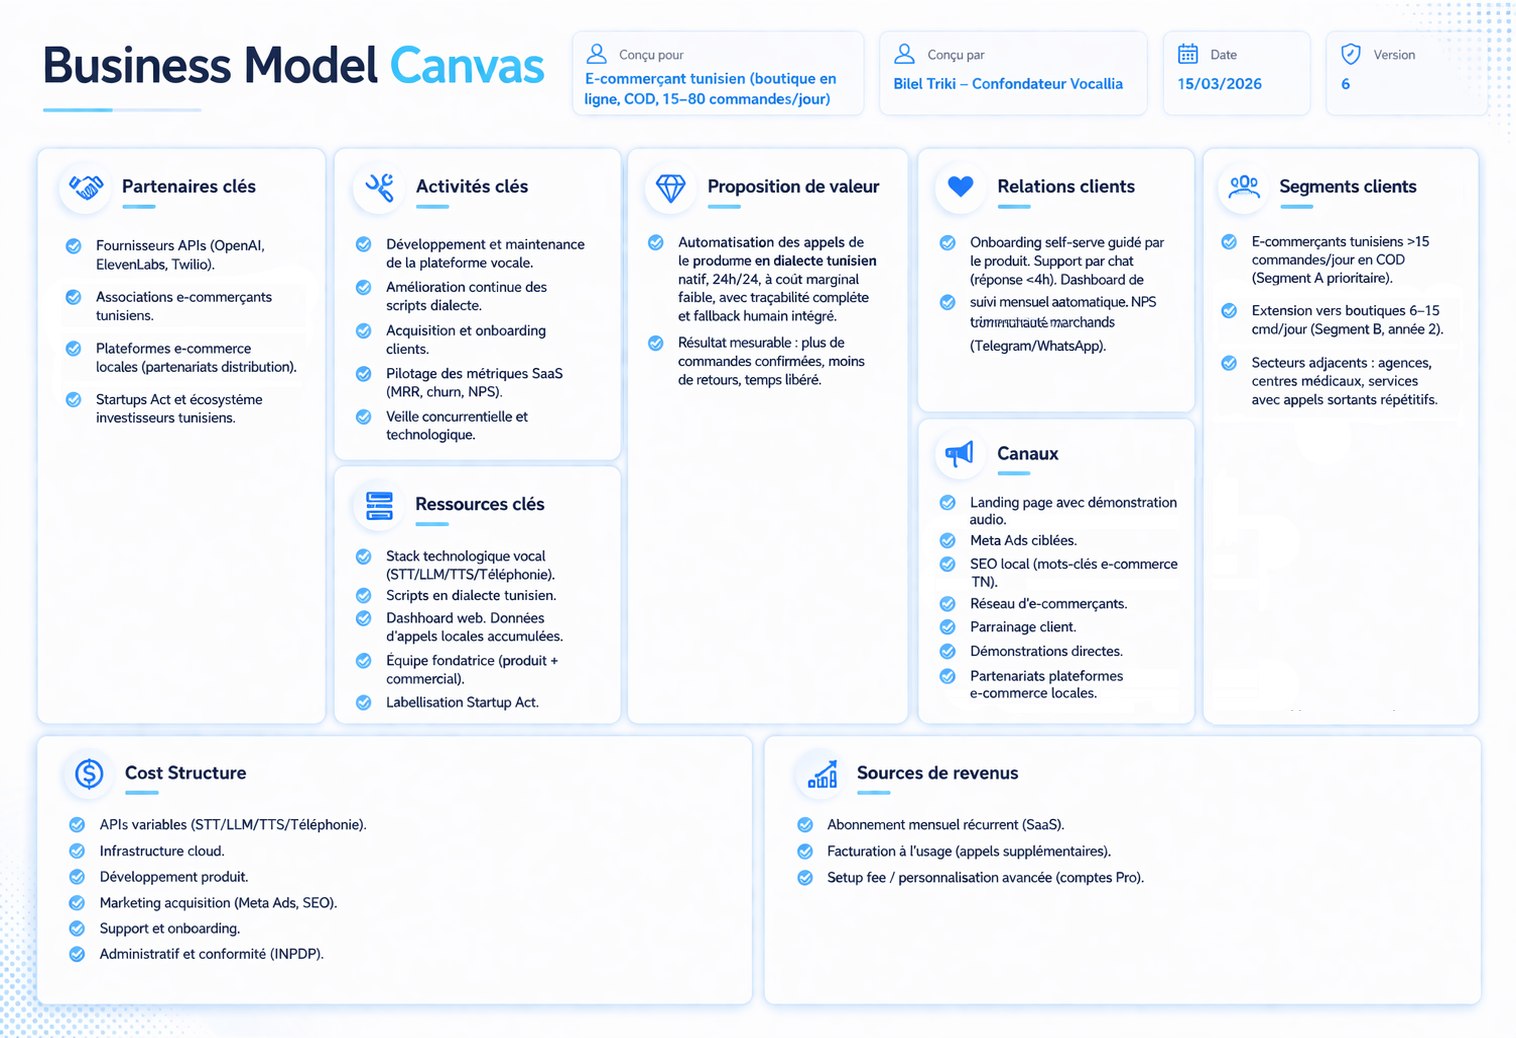
\includegraphics[width=\textwidth]{figures/bmc-vocallia.png}
    \caption{Business Model Canvas de Vocallia}
    \label{fig:bmc-vocallia}
\end{figure}

Les neuf blocs du BMC se résument comme suit. Les \textbf{segments de clientèle} ciblent en priorité les e-commerçants tunisiens à fort volume COD (Segment A), avec une extension vers les PME de services en année 2. La \textbf{proposition de valeur} repose sur l'automatisation des appels de confirmation en dialecte tunisien, avec dashboard de suivi intégré. Les \textbf{canaux} combinent vente directe B2B, acquisition digitale (Meta Ads, SEO) et réseau de partenaires. La \textbf{relation client} est conçue pour être majoritairement auto-gérée par le produit : onboarding guidé, démonstration personnalisée, suivi via tableau de bord. Les \textbf{sources de revenus} comprennent les abonnements mensuels (trois paliers), la facturation à l'usage et les frais d'intégration Pro. Les \textbf{ressources clés} sont l'infrastructure vocale, les modèles IA adaptés au dialecte tunisien, et les compétences en développement et intégration. Les \textbf{activités clés} couvrent le développement de la plateforme, l'amélioration continue des scripts, l'intégration e-commerce et l'acquisition client. Les \textbf{partenaires clés} --- OpenAI, ElevenLabs, Twilio --- sont gérés via une architecture multi-fournisseurs substituable. La \textbf{structure de coûts} est dominée par les variables (APIs), avec des coûts fixes limités à l'infrastructure cloud et au développement.

\medskip
\noindent\textbf{Lecture analytique du BMC.} Le modèle tient par un alignement fort entre trois blocs : la proposition de valeur répond à un problème structurel (confirmation COD), quotidien, et directement monétisable ; les canaux sont peu coûteux et empiriquement validés (CPL de 0,36~\euro{} en phase Muvaka) ; la relation client est conçue pour être auto-gérée par le produit, ce qui rend le modèle opérable avec une équipe de deux personnes en phase d'amorçage. La structure de coûts, dominée par les variables (APIs), confère au modèle sa propriété la plus précieuse : la scalabilité sans dégradation de marge. Le principal risque structurel est la concentration des partenaires clés --- trois fournisseurs d'APIs dont la défaillance ou la hausse tarifaire impacterait directement la rentabilité. L'architecture multi-fournisseurs, intégrée dès la conception, en est la réponse.

Le modèle étant structurellement viable, la section suivante en déploie les leviers opérationnels.

%%%%%%%%%%%%%%%%%%%%%%%%%%%%%%%%%%%%%%%%%%%%%%%%%%%%%%%%%%%%%%%%%%%%%%%%%%%
\section{Stratégie marketing opérationnelle --- cadre 8P}
\label{section3.6}
%%%%%%%%%%%%%%%%%%%%%%%%%%%%%%%%%%%%%%%%%%%%%%%%%%%%%%%%%%%%%%%%%%%%%%%%%%%

\subsection{Plan marketing opérationnel --- Marketing mix 8P}

Le plan marketing opérationnel de Vocallia s'articule autour du cadre élargi des
huit leviers du marketing mix (8P), développé à partir du modèle de
McCarthy (1960) et enrichi par Booms et Bitner (1981) pour les services.
Ce cadre structure les décisions opérationnelles de Vocallia selon trois
dimensions indissociables : la dimension technologique (solution SaaS), la
dimension de service (automatisation conversationnelle) et la dimension
relationnelle (accompagnement des e-commerçants tunisiens). Chaque levier
est décliné en décisions précises, actions concrètes et indicateurs mesurables.

% ------------------------------------------------------------
\subsubsection{Produit (\textit{Product}) --- Une infrastructure vocale intelligente,
pas un simple outil}
% ------------------------------------------------------------

\paragraph{Positionnement produit.}
Vocallia n'est pas un chatbot vocal générique. C'est une infrastructure
d'automatisation conversationnelle spécialisée, conçue pour un cas d'usage
précis --- la confirmation téléphonique des commandes e-commerce --- dans un
contexte linguistique spécifique, le dialecte tunisien avec code-switching
arabe/français. Cette spécialisation, cohérente avec le positionnement défini en
section~\ref{section3.2}, constitue le premier avantage concurrentiel défendable
du produit.

\paragraph{Architecture fonctionnelle.}
Le produit repose sur un pipeline vocal en cinq étapes séquentielles :
\begin{enumerate}
    \item \textbf{Déclenchement automatique} : à la réception d'une commande via
    webhook (Shopify, WooCommerce, API personnalisée), l'agent Vocallia initie
    l'appel sortant sans intervention humaine.
    \item \textbf{Reconnaissance vocale} (\textit{Speech-to-Text}) : conversion
    de la réponse du client en texte, via Whisper (OpenAI) avec ajustements pour
    le dialecte tunisien.
    \item \textbf{Compréhension et décision} (\textit{LLM}) : analyse de
    l'intention du client (confirmation, annulation, demande d'information,
    silence), génération de la réponse adaptée.
    \item \textbf{Synthèse vocale} (\textit{Text-to-Speech}) : conversion du
    texte généré en voix naturelle via ElevenLabs ou Azure Neural TTS.
    \item \textbf{Remontée des résultats} : mise à jour du statut de commande
    dans le système du marchand, notification en temps réel sur le tableau de bord.
\end{enumerate}

\paragraph{Offre produit structurée en trois paliers.}
La gamme est conçue selon une logique de \textit{good-better-best}, permettant à
chaque segment de trouver une entrée adaptée à son volume et à ses besoins :

\begin{itemize}
    \item \textbf{Plan Starter (79~DT/mois)} : 100~appels inclus, dialecte
    tunisien natif, dashboard de base, intégration webhook standard. Conçu pour
    les boutiques traitant 5 à 15~commandes par jour.
    \item \textbf{Plan Croissance (149~DT/mois)} : 300~appels inclus, dashboard
    complet avec export, rapports hebdomadaires automatiques, support prioritaire.
    Pour les boutiques à 15--50~commandes par jour.
    \item \textbf{Plan Pro (299~DT/mois)} : 800~appels inclus, intégration CRM
    avancée, scripts conversationnels personnalisés, rapport mensuel analytique,
    account manager dédié. Pour les structures à fort volume ($>$~50~commandes/jour).
\end{itemize}

\paragraph{Roadmap produit.}
Au-delà du cas d'usage initial (confirmation de commande), la feuille de route
produit prévoit l'extension vers d'autres scénarios conversationnels : relance
après abandon de panier (trimestre~3), rappel de rendez-vous pour les secteurs
de la santé et des services (année~2), qualification de leads entrants (année~2),
et service après-vente automatisé (année~3). Cette vision multi-cas d'usage
renforce la valeur à long terme du produit et réduit le risque de dépendance à
un unique segment.

\paragraph{Métriques produit.}
Les indicateurs de performance produit suivis sont : le taux de confirmation par
appel (objectif~$>$~70~\%), la durée moyenne d'appel (objectif~$<$~90~secondes),
la latence de réponse de l'agent (objectif~$<$~800~ms), le taux de déviation vers
un agent humain (objectif~$<$~15~\%), et le Net Promoter Score mensuel collecté
auprès des marchands (objectif~$>$~40).

% ------------------------------------------------------------
\subsubsection{Prix (\textit{Price}) --- Un pricing ancré sur la valeur créée,
pas sur les coûts}
% ------------------------------------------------------------

\paragraph{Philosophie tarifaire.}
La stratégie de prix de Vocallia est fondée sur la valeur créée pour le client,
et non sur une logique de coût majoré. Cette approche, recommandée pour les
startups SaaS B2B en phase d'amorçage (Anderson et al., \textit{Value-Based
Pricing}, 2010), permet de capturer une part de la valeur générée plutôt que
de se positionner sur la seule compétitivité tarifaire --- et donc de protéger
la marge à mesure que les coûts d'API diminuent.

\paragraph{Justification économique du pricing côté fournisseur.}
Le coût variable total d'un appel de deux minutes est estimé à environ 0,27~DT
(cf. figure~\ref{fig:cout_appel}). Sur cette base,
le plan Starter (79~DT pour 100~appels, soit 0,79~DT par appel) génère une marge
brute d'environ 65,3~\%. Ce niveau demeure élevé pour une offre SaaS en phase
d'amorçage, tout en préservant une structure de coûts compatible avec la scalabilité
du modèle.

\paragraph{Justification économique côté client.}
Pour un marchand traitant 150~commandes par mois avec un taux de retour de 15~\%
et un coût logistique de 12~DT par retour non anticipé, le coût mensuel
des retours s'élève à 270~DT. Si Vocallia réduit ce taux de 30~\% --- hypothèse
conservatrice basée sur l'amélioration du taux de joignabilité --- l'économie
mensuelle atteint 81~DT, soit davantage que le plan Starter (79~DT). L'abonnement
s'autofinance par la seule réduction des pertes logistiques, sans même comptabiliser
le temps opérationnel libéré pour le gérant.

\paragraph{Politique tarifaire complémentaire.}
En complément de l'abonnement mensuel, deux mécanismes tarifaires sont prévus :
\begin{itemize}
    \item \textbf{Appels supplémentaires} : facturation unitaire au-delà du
    forfait (0,90~DT/appel pour Starter, 0,70~DT pour Croissance, 0,50~DT pour
    Pro), alignant le coût marginal sur la valeur créée.
    \item \textbf{Setup fee} : frais uniques de configuration pour le plan Pro
    (500~DT), couvrant le paramétrage du CRM, la personnalisation des scripts et
    la formation initiale du marchand.
\end{itemize}

\paragraph{Pilote d'entrée sans engagement.}
Une offre d'entrée à risque nul complète le dispositif : 50~appels gratuits sur les vraies
commandes du client, sans carte bancaire requise. Ce mécanisme, inspiré du
modèle \textit{Product-Led Growth} (Wuebben, 2021), supprime la barrière
psychologique à l'entrée et permet au produit de se vendre lui-même avant
toute transaction commerciale.

% ------------------------------------------------------------
\subsubsection{Distribution (\textit{Place}) --- Un modèle 100~\% digital,
pensé pour une adoption sans friction}
% ------------------------------------------------------------

\paragraph{Canal unique : SaaS cloud.}
La distribution de Vocallia est entièrement dématérialisée. Il n'existe pas de
version physique du produit, pas de déplacement commercial requis, et pas
d'installation locale nécessaire dans la configuration standard. Cette approche
est cohérente avec le profil des clients cibles --- des e-commerçants actifs en
ligne --- et avec les contraintes budgétaires d'une startup en amorçage.

\paragraph{Parcours d'activation client.}
Le parcours complet d'un nouveau client se déroule en quatre étapes, toutes
réalisables sans contact humain :
\begin{enumerate}
    \item \textbf{Inscription} sur la landing page (email + numéro de téléphone),
    accès immédiat au pilote gratuit.
    \item \textbf{Configuration guidée} : assistant d'onboarding en 5~étapes
    pour connecter la source de commandes (webhook ou import CSV).
    \item \textbf{Activation} : premier appel envoyé automatiquement dès la
    réception d'une commande de test. Temps de mise en service cible~: moins de
    20~minutes.
    \item \textbf{Upgrade} : proposition automatique de passage au plan payant
    après consommation des 50~appels gratuits, avec affichage du résultat
    obtenu pendant le pilote.
\end{enumerate}

\paragraph{Déploiement géographique progressif.}
La stratégie de distribution suit une logique de concentration géographique
initiale, privilégiant les gouvernorats à forte densité de e-commerçants :
Grand Tunis (Tunis, Ariana, Ben Arous, Manouba) en priorité, suivi de Sfax et
Sousse en phase 2. Cette concentration permet d'optimiser les efforts de
support et de construire des effets de réseau locaux (bouche-à-oreille entre
marchands d'un même secteur géographique).

\paragraph{Option déploiement on-premise.}
Pour les secteurs sensibles (banque, santé, assurances), une option de
déploiement sur infrastructure privée est documentée et proposée sur devis.
Cette flexibilité architecturale répond aux exigences de souveraineté des
données et constitue un argument commercial différenciant pour les comptes Pro.

% ------------------------------------------------------------
\subsubsection{Communication (\textit{Promotion}) --- Une stratégie de preuve
à faible coût d'acquisition}
% ------------------------------------------------------------

\paragraph{Philosophie de communication.}
La stratégie de communication repose sur un principe central :
\textbf{montrer plutôt que promettre}. Dans un marché où la méfiance envers les
promesses technologiques est réelle, chaque canal est conçu comme un vecteur
de preuve concrète --- un extrait d'appel réel vaut plus que dix arguments.

\paragraph{Canal 1 --- Meta Ads (Facebook / Instagram).}
Les campagnes publicitaires Meta constituent le canal d'acquisition principal
en phase de lancement. Les données de la phase exploratoire Muvaka (avril~2025)
ont démontré la viabilité de ce canal : coût par lead de 0,36~\euro{} pour un budget
de 10~\euro{}, taux de clic de 10,9~\% sur la campagne Website Visit --- des résultats
significativement plus favorables que les benchmarks B2B habituels sur
Meta Ads (3--15~\euro{} par lead).

La stratégie publicitaire est structurée en trois phases~:
\begin{itemize}
    \item \textbf{Phase Teasing (semaines~1--2)} : vidéo courte (15~secondes)
    montrant un extrait d'appel IA en dialecte tunisien, sans révéler le produit.
    Objectif : générer la curiosité et mesurer l'engagement.
    \item \textbf{Phase Lancement (semaines~3--6)} : campagne Leads avec
    formulaire intégré proposant le pilote gratuit. Ciblage : e-commerçants
    tunisiens, 25--45~ans, intérêts e-commerce et business.
    \item \textbf{Phase Rétention (mois~2 et au-delà)} : retargeting des
    visiteurs non convertis, témoignages clients pilotes, contenu éducatif sur
    la valeur de l'automatisation vocale.
\end{itemize}

\paragraph{Canal 2 --- Content marketing et SEO local.}
Une stratégie de contenu éducatif est déployée sur deux supports~:
\begin{itemize}
    \item \textbf{Blog Vocallia} : articles optimisés pour le référencement
    naturel sur des requêtes spécifiques (exemples : \og{}automatiser les appels
    commande Tunisie\fg{}, \og{}réduire les retours colis e-commerce\fg{}, \og{}agent IA
    tunisien\fg{}). Objectif~: capter le trafic en phase de recherche active sans
    coût publicitaire.
    \item \textbf{Vidéos tutoriels} (YouTube / Facebook) : démonstrations
    pratiques de l'interface Vocallia, cas d'usage filmés avec de vrais marchands,
    FAQ en dialecte tunisien. Ces formats répondent aux objections les plus
    fréquentes identifiées dans l'étude terrain (\og{}est-ce que l'IA parle vraiment
    tunisien~?\fg{}, \og{}comment mes clients vont réagir~?\fg{}).
\end{itemize}

\paragraph{Canal 3 --- Démonstration directe.}
Le mécanisme de conversion le plus puissant est la démonstration en temps réel :
lors d'un premier contact, l'équipe déclenche un appel vers le téléphone du
prospect, simulant une confirmation de commande en dialecte tunisien. L'effet
de surprise et la naturalité de l'échange court-circuitent les objections
rationnelles --- c'est le moment de bascule identifié par les personas.

\paragraph{Canal 4 --- Programme de parrainage (\textit{referral}).}
Un mécanisme de recommandation structuré est mis en place dès le premier mois
d'activité~: tout client actif ayant recommandé Vocallia à un autre marchand
bénéficie d'un mois offert (valeur~: 79 à 299~DT selon son plan), et le filleul
reçoit son pilote étendu à 100~appels au lieu de 50. Ce mécanisme exploite la
dynamique communautaire des e-commerçants tunisiens, qui partagent activement
leurs pratiques opérationnelles dans des groupes Facebook et WhatsApp dédiés.

\paragraph{Canal 5 --- Partenariats éducatifs et institutionnels.}
Des partenariats sont développés avec les structures d'accompagnement des
entrepreneurs numériques tunisiens~: incubateurs (Flat6Labs, StartupBootcamp
Africa), associations d'e-commerçants, chambres de commerce régionales. Ces
partenariats permettent d'accéder à des audiences qualifiées sans coût
publicitaire direct et renforcent la crédibilité institutionnelle du projet.

% ------------------------------------------------------------
\subsubsection{Personnel (\textit{People}) --- Une équipe restreinte,
un produit qui assume le rôle commercial}
% ------------------------------------------------------------

\paragraph{Structure initiale de l'équipe.}
En cohérence avec le modèle \textit{Product-Led Growth} adopté, l'équipe
commerciale de Vocallia est volontairement restreinte en phase d'amorçage.
Le produit lui-même assume une grande partie du rôle commercial~: l'onboarding
est automatisé, la preuve de valeur est intégrée au pilote, et la
conversion est déclenchée par le dashboard de suivi des résultats.

L'équipe initiale se compose de~:
\begin{itemize}
    \item \textbf{Le porteur de projet} (CEO) : vision stratégique, développement
    commercial, gestion des partenariats, démonstrations directes auprès des
    prospects prioritaires.
    \item \textbf{Le co-fondateur technique} (CTO) : développement et maintenance
    du pipeline vocal, gestion des API, amélioration continue des modèles.
    \item \textbf{Support client} (freelance ou temps partiel, à partir du
    mois~3) : onboarding des nouveaux clients, réponse aux questions techniques,
    suivi des comptes Pro.
\end{itemize}

\paragraph{Formation et qualité de service.}
L'ensemble de l'équipe est formé sur les spécificités de la relation client
B2B dans le contexte tunisien~: compréhension des cycles de décision des PME,
maîtrise des objections liées à l'IA vocale, capacité à réaliser une
démonstration produit en conditions réelles. Un guide de vente interne est
rédigé et mis à jour mensuellement, intégrant les nouvelles objections rencontrées
sur le terrain et les réponses les plus efficaces.

\paragraph{Évolution de l'équipe.}
La croissance de l'équipe est conditionnée à l'atteinte des jalons commerciaux~:
recrutement d'un commercial terrain au-delà de 50~clients actifs, recrutement
d'un chargé de \textit{customer success} au-delà de 100~clients actifs.

% ------------------------------------------------------------
\subsubsection{Processus (\textit{Process}) --- Minimiser le délai entre
la découverte et la première preuve de valeur}
% ------------------------------------------------------------

\paragraph{Cartographie du parcours client.}
Le processus client de Vocallia est conçu pour minimiser le \textit{Time to Value}
(TTV) --- le délai entre la découverte du produit et la première preuve de valeur
perçue par le client. Cet indicateur est critique pour la rétention~: plus il
est court, plus le taux de conversion du pilote vers le plan payant est élevé
(OpenView Partners, \textit{PLG Benchmark}, 2024).

Le parcours se décompose en sept étapes mesurées~:

\begin{enumerate}
    \item \textbf{Découverte} (publicité, bouche-à-oreille, SEO) $\rightarrow$ atterrissage
    sur la landing page.
    \item \textbf{Inscription} (email + téléphone) $\rightarrow$ accès immédiat au tableau
    de bord. Durée cible~: moins de 2~minutes.
    \item \textbf{Configuration} (connexion de la source de commandes)
    $\rightarrow$ assistant guidé en 5~étapes. Durée cible~: moins de 15~minutes.
    \item \textbf{Premier appel} $\rightarrow$ déclenché automatiquement sur la prochaine
    commande reçue. Durée cible depuis l'inscription~: moins de 24~heures.
    \item \textbf{Consultation du tableau de bord} $\rightarrow$ visualisation des résultats.
    Premier signal de rétention~: le client revient consulter son dashboard.
    \item \textbf{Consommation du pilote} (50~appels) $\rightarrow$ proposition automatique
    d'upgrade avec affichage des résultats obtenus.
    \item \textbf{Conversion payante} $\rightarrow$ choix du plan adapté au volume, activation
    de la facturation.
\end{enumerate}

\paragraph{Gestion des cas d'erreur.}
Tout scénario d'appel qui dépasse les capacités de l'agent IA déclenche
automatiquement une notification au marchand (SMS + notification dashboard) avec
le détail de l'échange et la recommandation d'un rappel humain. Ce mécanisme
de \textit{graceful fallback} garantit qu'aucune commande n'est perdue en cas
de limitation de l'IA et renforce la confiance du marchand dans le système.

\paragraph{Processus d'amélioration continue.}
Les transcriptions d'appels (anonymisées, avec consentement) alimentent un
cycle d'amélioration mensuel : identification des patterns d'échec, mise à jour
des scripts, test A/B sur un sous-ensemble de clients. Ce processus crée un
avantage cumulatif --- chaque appel enrichit le corpus local --- que les
concurrents entrants ne pourront pas répliquer instantanément.

% ------------------------------------------------------------
\subsubsection{Preuves physiques (\textit{Physical Evidence}) --- Rendre
visible et mesurable la valeur créée}
% ------------------------------------------------------------

\paragraph{Le défi des services immatériels.}
L'un des défis fondamentaux de la commercialisation d'un service IA est son
caractère immatériel : le client ne voit pas l'agent travailler, il ne perçoit
que les résultats. Les \textit{physical evidences} --- preuves tangibles de
la qualité du service --- jouent un rôle critique pour instaurer la
confiance (Zeithaml et al., \textit{Services Marketing}, 2018) et constituent
le mécanisme de rétention principal de Vocallia.

\paragraph{Tableau de bord comme preuve principale.}
Le dashboard Vocallia est conçu comme l'interface de confiance principale du
marchand. Il doit répondre à une question fondamentale en moins de 10~secondes~:
\og{}est-ce que Vocallia m'a été utile ce mois-ci~?\fg{} Pour cela, il affiche en
premier plan quatre indicateurs clés~: commandes confirmées automatiquement,
temps opérationnel libéré, retours potentiellement évités, et taux de
joignabilité des clients.

\paragraph{Rapport mensuel automatique.}
À la fin de chaque mois, un rapport synthétique est généré et envoyé par email
au marchand. Ce document d'une page présente les métriques clés du mois, la
comparaison avec le mois précédent, et une recommandation automatique
(augmenter le volume d'appels, étendre à d'autres cas d'usage, passer au palier
supérieur). Ce rapport crée un rendez-vous mensuel régulier entre Vocallia et
son client, renforçant l'ancrage de la solution dans les habitudes opérationnelles
et réduisant le risque de churn passif.

\paragraph{Transcriptions et enregistrements.}
Chaque appel génère une transcription consultable dans le tableau de bord.
Le marchand peut écouter l'appel, lire la transcription et vérifier que l'échange
a été conduit conformément à ses attentes. Cette transparence totale est à la
fois une preuve de qualité et un outil d'ajustement~: si le marchand identifie
une formulation inadaptée, il peut la signaler et demander une mise à jour du script.

% ------------------------------------------------------------
\subsubsection{Partenariats (\textit{Partners}) --- Construire un écosystème
de crédibilité et d'accès}
% ------------------------------------------------------------

\paragraph{Partenaires technologiques.}
Les partenaires technologiques de Vocallia sont les fournisseurs d'API qui
constituent le pipeline vocal~: OpenAI (Whisper et GPT-4o-mini), ElevenLabs
(synthèse vocale), Twilio (téléphonie). Ces partenariats sont gérés selon une
architecture multi-fournisseurs permettant la substitution rapide d'un provider
en cas de hausse tarifaire ou d'interruption de service, limitant la
dépendance stratégique identifiée dans l'analyse SWOT.

\paragraph{Partenaires commerciaux.}
Deux catégories de partenaires commerciaux sont ciblées~:
\begin{itemize}
    \item \textbf{Plateformes e-commerce locales} (agrégateurs de boutiques
    tunisiennes, prestataires de logistique e-commerce) qui peuvent référencer
    Vocallia comme solution complémentaire. Un accord de \textit{referral} est
    proposé~: commission de 15~\% sur la première année de chaque client apporté.
    \item \textbf{Agences digitales et consultants} accompagnant des e-commerçants
    tunisiens dans leur transformation numérique. Ces intermédiaires ont une
    relation de confiance avec les marchands et peuvent recommander Vocallia
    dans le cadre d'une offre de service élargie.
\end{itemize}

\paragraph{Partenaires institutionnels.}
Des partenariats sont développés avec les structures d'appui à l'entrepreneuriat
numérique~: Startup Act (labellisation et accès aux avantages fiscaux),
incubateurs (Flat6Labs Tunisia, Cogite), associations professionnelles des
e-commerçants tunisiens. Ces partenariats renforcent la légitimité du projet
et ouvrent des accès à des réseaux qualifiés.

\paragraph{Tableau de synthèse --- plan marketing opérationnel 8P.}

\begin{figure}[H]
    \centering
    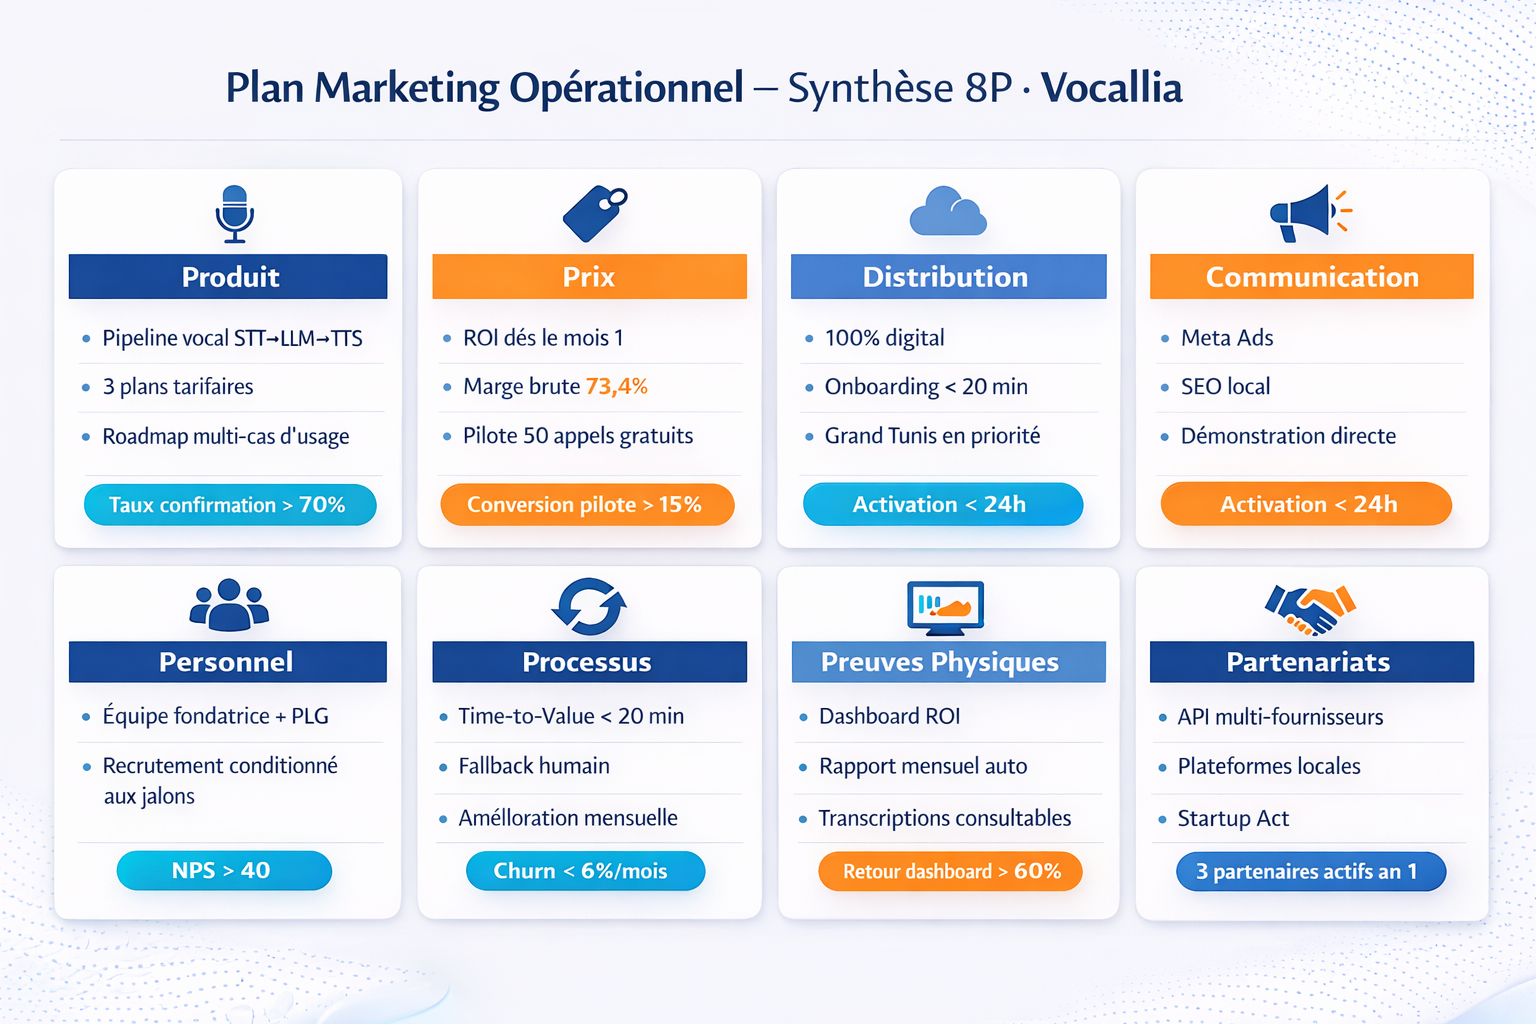
\includegraphics[width=\textwidth]{figures/marketing_8p_vocallia.png}
    \caption{Synthèse du plan marketing opérationnel Vocallia (8P)}
    \label{fig:marketing_8p}
\end{figure}

\medskip
Les huit leviers étant définis, la section suivante en organise le déploiement séquentiel à travers la stratégie go-to-market et le tunnel de conversion.

%%%%%%%%%%%%%%%%%%%%%%%%%%%%%%%%%%%%%%%%%%%%%%%%%%%%%%%%%%%%%%%%%%%%%%%%%%%
\section{Stratégie go-to-market et tunnel commercial}
\label{section3.7}
%%%%%%%%%%%%%%%%%%%%%%%%%%%%%%%%%%%%%%%%%%%%%%%%%%%%%%%%%%%%%%%%%%%%%%%%%%%

La stratégie go-to-market de Vocallia s'appuie sur le modèle Product-Led Growth (PLG), dans lequel le produit lui-même --- et non une force de vente --- constitue le principal vecteur d'acquisition, de conversion et de rétention. Ce modèle, adopté par 58~\% des entreprises B2B SaaS en 2024 (OpenView Partners, 2024), est le seul viable dans le contexte de Vocallia : budget marketing limité, marché de PME qui exigent une preuve avant tout engagement, et nécessité de convertir rapidement les marchands du Segment A pour atteindre le seuil de rentabilité identifié dans les projections.

%%%%%%%%%%%%%%%%%%%%%%%%%%%%%%%%%%%%%%%%%%%%%%%%%%%%%%%%%%%%%%%%%%%%%%%%%%%
\subsection{Entonnoir de conversion PLG}
\label{section3.7.1}
%%%%%%%%%%%%%%%%%%%%%%%%%%%%%%%%%%%%%%%%%%%%%%%%%%%%%%%%%%%%%%%%%%%%%%%%%%%

\begin{table}[H]
\centering
\caption{Entonnoir de conversion PLG --- Vocallia}
\vspace{4pt}
\begin{tabularx}{\textwidth}{|>{\raggedright\arraybackslash}p{2cm}|>{\raggedright\arraybackslash}X|>{\raggedright\arraybackslash}X|>{\raggedright\arraybackslash}p{2.2cm}|}
\hline
\textbf{Étape} & \textbf{Mécanisme} & \textbf{Objectif} & \textbf{KPI cible} \\
\hline
Découverte & Meta Ads ciblées (e-commerçants TN), SEO local, bouche à oreille réseau & Générer des leads qualifiés à faible coût & CPL $<$ 5 DT \\
\hline
Intérêt & Landing page avec démonstration audio d'un appel réel en dialecte tunisien & Créer le déclic \og{}ça marche vraiment en tunisien\fg{} & Conv. LP $>$ 8~\% \\
\hline
Activation & 50 appels gratuits sans engagement sur les vraies commandes du client & Prouver la valeur sur données réelles & Activation $>$ 70~\% \\
\hline
Conversion & Dashboard affichant les résultats chiffrés du pilote en DT & Transformer les données en décision d'achat & Free-to-paid $>$ 15~\% \\
\hline
Rétention & Rapport mensuel automatique, NPS, amélioration continue des scripts & Ancrer l'usage et réduire le churn & Churn mensuel $<$ 6~\% \\
\hline
Expansion & Upsell vers palier supérieur si volume dépassé. Recommandation à d'autres marchands. & Croître via les clients existants & NRR $>$ 110~\% \\
\hline
\end{tabularx}
\end{table}


%%%%%%%%%%%%%%%%%%%%%%%%%%%%%%%%%%%%%%%%%%%%%%%%%%%%%%%%%%%%%%%%%%%%%%%%%%%
\subsection{Tunnel commercial détaillé}
\label{section3.7.2}
%%%%%%%%%%%%%%%%%%%%%%%%%%%%%%%%%%%%%%%%%%%%%%%%%%%%%%%%%%%%%%%%%%%%%%%%%%%

L'entonnoir PLG se déploie opérationnellement en un tunnel commercial en six phases, chacune conçue pour réduire l'incertitude du marchand à chaque étape et le rapprocher de la conversion par les faits, pas par le discours.

\textbf{Phase 1 --- Prospection.} Identification des e-commerçants actifs à fort volume COD via Meta Ads, groupes Facebook e-commerce tunisiens, réseaux professionnels locaux. Critères de qualification : $>$15 commandes/jour, COD dominant, gérant joignable. Objectif : 20 à 30 leads qualifiés par mois en régime de croisière.

\textbf{Phase 2 --- Qualification.} Contact initial par message personnalisé, avec une question d'accroche centrée sur le problème : \og{}Combien de commandes perdez-vous par semaine faute d'avoir pu rappeler à temps ?\fg{}. Le taux de réponse à ce type de message orienté problème est supérieur à un discours centré sur les fonctionnalités.

\textbf{Phase 3 --- Démonstration.} Envoi d'un lien vers la landing page avec échantillon audio. Option : simulation en direct de 15 minutes sur un script adapté au profil du marchand. C'est le point de bascule --- en quelques secondes, la naturalité de la voix en dialecte tunisien dissipe les objections.

\textbf{Phase 4 --- Pilote.} Activation des 50 appels gratuits. Le marchand fournit ses premières commandes du jour. Vocallia confirme en automatique. Le fondateur reste disponible pour un suivi quotidien pendant les 7 premiers jours.

\textbf{Phase 5 --- Closing.} Présentation du dashboard à la fin du pilote : appels effectués, taux de confirmation, économies estimées en DT. La conversion est déclenchée par les chiffres du client lui-même. Proposition du plan adapté au volume observé.

\textbf{Phase 6 --- Onboarding et expansion.} Configuration complète des scripts, intégration CRM si applicable, formation au dashboard. À 90 jours, déclenchement de la demande de témoignage et de recommandation. À 6 mois, analyse de la montée en charge et proposition d'upsell vers le palier supérieur.

\medskip
La stratégie go-to-market étant définie, les sections suivantes en vérifient la viabilité financière. C'est ici que la démonstration de viabilité commerciale atteint son point culminant : la politique tarifaire prouve que le pricing est simultanément attractif et rentable ; les unit economics prouvent que le modèle d'acquisition est soutenable à l'échelle ; les projections financières prouvent que l'ensemble converge vers la rentabilité dans un délai maîtrisé.

%%%%%%%%%%%%%%%%%%%%%%%%%%%%%%%%%%%%%%%%%%%%%%%%%%%%%%%%%%%%%%%%%%%%%%%%%%%
\section{Stratégie de tarification}
\label{section3.8}
%%%%%%%%%%%%%%%%%%%%%%%%%%%%%%%%%%%%%%%%%%%%%%%%%%%%%%%%%%%%%%%%%%%%%%%%%%%

La politique de prix est le point de convergence de toute la stratégie commerciale : c'est elle qui traduit la proposition de valeur en transaction et qui détermine si le modèle est simultanément attractif pour le client, rentable pour Vocallia, et crédible face aux investisseurs. Le pricing est construit à partir de trois contraintes simultanées : la sensibilité prix déclarée sur le terrain, le coût unitaire réel par appel, et les ratios de référence de l'industrie SaaS. Ce triple ancrage élimine le risque d'un pricing arbitraire.

%%%%%%%%%%%%%%%%%%%%%%%%%%%%%%%%%%%%%%%%%%%%%%%%%%%%%%%%%%%%%%%%%%%%%%%%%%%
\subsection{Grille tarifaire --- trois paliers}
\label{section3.8.1}
%%%%%%%%%%%%%%%%%%%%%%%%%%%%%%%%%%%%%%%%%%%%%%%%%%%%%%%%%%%%%%%%%%%%%%%%%%%

\begin{table}[H]
\centering
\caption{Grille tarifaire Vocallia --- trois paliers}
\vspace{4pt}
\begin{tabularx}{\textwidth}{|>{\raggedright\arraybackslash}p{3.2cm}|>{\raggedright\arraybackslash}X|>{\raggedright\arraybackslash}X|>{\raggedright\arraybackslash}X|}
\hline
& \textbf{Starter} & \textbf{Croissance} & \textbf{Pro} \\
\hline
Prix mensuel & \textbf{79 DT} & \textbf{149 DT} & \textbf{299 DT} \\
\hline
Appels inclus/mois & 100 appels & 300 appels & 800 appels \\
\hline
Appel supplémentaire & 0,90 DT/appel & 0,70 DT/appel & 0,50 DT/appel \\
\hline
Dialecte tunisien & Oui & Oui & Oui \\
\hline
Dashboard & Basique & Complet & Complet $+$ export CSV \\
\hline
Intégration CRM & Non & Via webhook & Via webhook $+$ support dédié \\
\hline
Setup fee & Offert & Offert & 500 DT (unique) \\
\hline
Profil cible & Boutiques 5--15 cmd/jour & Boutiques 15--50 cmd/jour & Boutiques $>$50 cmd/jour \\
\hline
\end{tabularx}
\end{table}


%%%%%%%%%%%%%%%%%%%%%%%%%%%%%%%%%%%%%%%%%%%%%%%%%%%%%%%%%%%%%%%%%%%%%%%%%%%
\subsection{Justification économique du pricing}
\label{section3.8.2}
%%%%%%%%%%%%%%%%%%%%%%%%%%%%%%%%%%%%%%%%%%%%%%%%%%%%%%%%%%%%%%%%%%%%%%%%%%%

\noindent\textbf{Côté fournisseur --- marge brute.} Pour le plan Starter (79 DT / 100 appels) : coût variable $=$ 100 $\times$ 0,21 DT $=$ 21 DT. Marge brute $=$ 58 DT, soit \textbf{73,4~\%} --- au-dessus du seuil de référence SaaS de 70~\% (Bessemer Venture Partners, State of the Cloud, 2024). Pour le plan Croissance (149 DT / 300 appels) : coût variable $=$ 63 DT. Marge brute $=$ 86 DT, soit \textbf{57,7~\%}, compensée par le volume supérieur et la moindre intensité de support par client. Le plan Pro (299 DT / 800 appels) atteint un coût variable de 168 DT et une marge brute de 43,8~\%, mais intègre le setup fee de 500 DT et la facturation des dépassements à 0,50 DT/appel, ce qui rétablit la rentabilité globale du compte. La marge brute pondérée du portefeuille, dominée par les plans Starter et Croissance en phase de lancement, se situe au-dessus de 65~\%.

\medskip
\noindent\textbf{Côté client --- valeur créée supérieure au coût.} Pour un marchand à 150 commandes/mois avec un taux de retour de 15~\% (12 DT par retour), une réduction de 30~\% du taux de retour génère une économie de 81 DT --- supérieure au plan Starter à 79 DT. L'abonnement s'autofinance par les seules économies logistiques, sans même comptabiliser les gains opérationnels indirects.

\begin{tcolorbox}[colback=gray!8, colframe=gray!50, title=\textbf{Formule de valeur --- outil de closing commercial}, fonttitle=\bfseries]
\textbf{Économie mensuelle Vocallia} $=$ Commandes/mois $\times$ Taux de retour $\times$ Coût par retour $\times$ Taux de réduction attendu

\medskip
\textbf{Exemple :} 150 commandes $\times$ 15~\% $\times$ 12 DT $\times$ 30~\% $=$ \textbf{81 DT économisés/mois}

Plan Starter $=$ 79 DT/mois $\Rightarrow$ \textbf{L'abonnement s'autofinance dès le premier mois.}

\medskip
\noindent Cette formule est intégrée au dashboard et calculée automatiquement sur les données réelles du client pendant le pilote. C'est elle --- et non un argumentaire commercial --- qui déclenche la conversion.
\end{tcolorbox}

%%%%%%%%%%%%%%%%%%%%%%%%%%%%%%%%%%%%%%%%%%%%%%%%%%%%%%%%%%%%%%%%%%%%%%%%%%%
\section{Unit economics SaaS --- viabilité financière du modèle}
\label{section3.9}
%%%%%%%%%%%%%%%%%%%%%%%%%%%%%%%%%%%%%%%%%%%%%%%%%%%%%%%%%%%%%%%%%%%%%%%%%%%

Les unit economics sont le test décisif de la viabilité d'un modèle SaaS : ils répondent à une question simple --- chaque client acquis génère-t-il davantage de valeur qu'il n'en coûte à conquérir et à servir~? La politique tarifaire a établi que la marge brute dépasse 65~\% en pondéré. Cette section vérifie que cette marge se traduit en un modèle d'acquisition soutenable à l'échelle --- et fournit les métriques que tout investisseur examinera en premier.

%%%%%%%%%%%%%%%%%%%%%%%%%%%%%%%%%%%%%%%%%%%%%%%%%%%%%%%%%%%%%%%%%%%%%%%%%%%
\subsection{Calcul des métriques clés}
\label{section3.9.1}
%%%%%%%%%%%%%%%%%%%%%%%%%%%%%%%%%%%%%%%%%%%%%%%%%%%%%%%%%%%%%%%%%%%%%%%%%%%

\begin{table}[H]
\centering
\caption{Unit economics SaaS --- métriques clés Vocallia (scénario réaliste)}
\vspace{4pt}
\begin{tabularx}{\textwidth}{|>{\raggedright\arraybackslash}p{2.3cm}|>{\raggedright\arraybackslash}X|>{\raggedright\arraybackslash}p{2.5cm}|>{\raggedright\arraybackslash}X|}
\hline
\textbf{Métrique} & \textbf{Définition} & \textbf{Valeur cible} & \textbf{Base de calcul} \\
\hline
ARPU & Revenu moyen mensuel par client actif & 120 DT/mois & Mix des 3 paliers, dominance plan Croissance \\
\hline
Churn mensuel & Taux d'attrition mensuel & 5 -- 8~\% & Benchmark SaaS B2B PME : 5--10~\%/mois \\
\hline
LTV & Valeur vie client (ARPU / churn) & 1\,500 -- 2\,400 DT & 120 / 0,08 à 120 / 0,05 \\
\hline
CAC & Coût d'acquisition d'un client payant & $<$ 150 DT & 0,36~\euro{}/lead $\times$ taux conv. 15~\% $\approx$ 2,4~\euro{}/client qualifié \\
\hline
Ratio LTV:CAC & Viabilité du modèle d'acquisition & 10:1 à 16:1 & Benchmark minimal SaaS : 3:1 \\
\hline
CAC Payback & Mois pour récupérer le CAC & $<$ 2 mois & CAC 150 DT / ARPU 120 DT \\
\hline
MRR cible An 1 & MRR en fin d'année 1 & 4\,800 -- 6\,000 DT & 40--50 clients $\times$ 120 DT \\
\hline
\end{tabularx}
\end{table}


\medskip
La figure~\ref{fig:ltv_cac} met en perspective le ratio LTV:CAC projeté de Vocallia par rapport aux benchmarks de référence de l'industrie SaaS.

\begin{figure}[H]
\centering
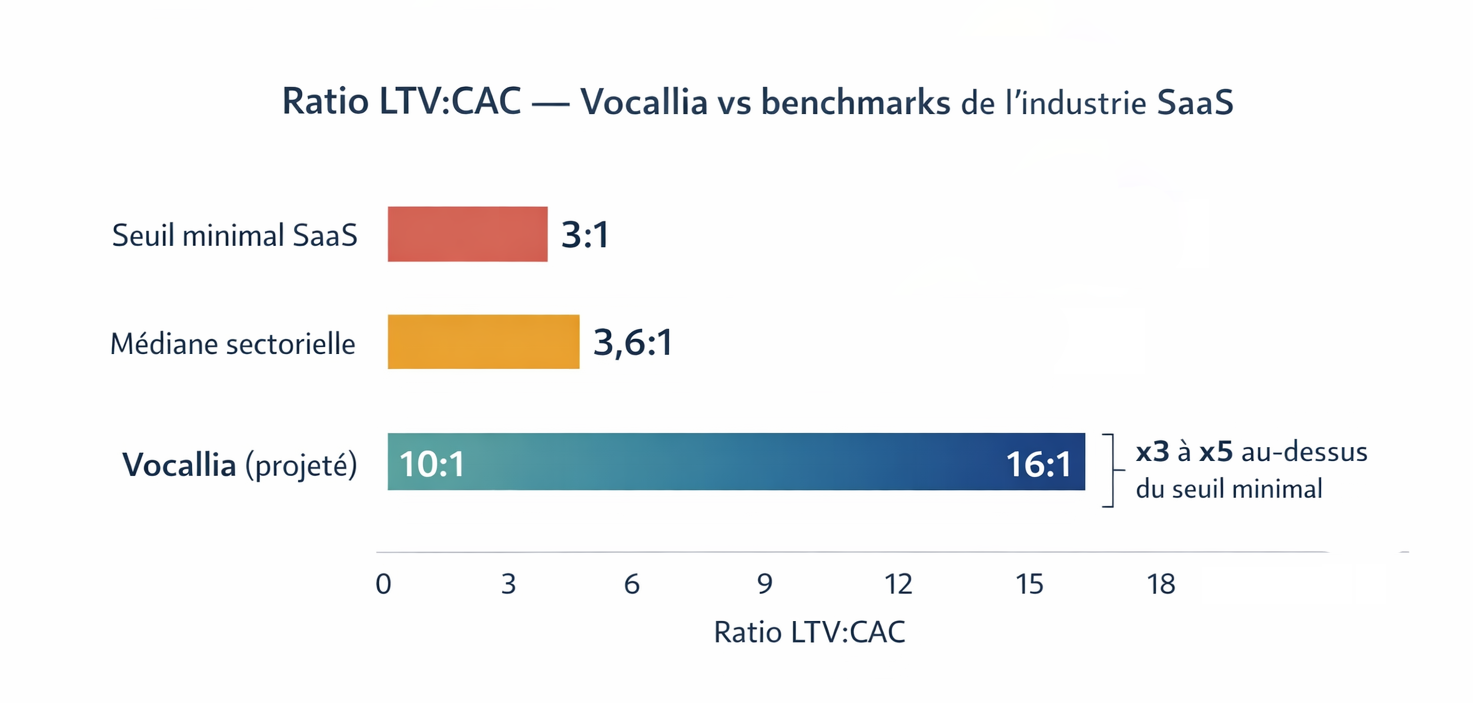
\includegraphics[width=0.92\textwidth]{figures/ltv_cac_benchmark.png}
\caption{Ratio LTV:CAC --- Vocallia vs benchmarks de l'industrie SaaS}
\label{fig:ltv_cac}
\end{figure}

\begin{tcolorbox}[colback=gray!8, colframe=gray!50, title=\textbf{Interprétation des unit economics}, fonttitle=\bfseries]
Un ratio LTV:CAC projeté entre 10:1 et 16:1 place Vocallia très au-dessus du seuil minimal de 3:1 recommandé par les investisseurs SaaS (Benchmarkit, 2024), et au-dessus de la médiane sectorielle de 3,6:1. Cette asymétrie repose sur deux caractéristiques structurelles du marché --- et non sur des hypothèses optimistes. Premièrement, le coût d'acquisition est empiriquement faible : le CPL de 0,36~\euro{} validé en phase Muvaka est 8 à 40 fois inférieur aux benchmarks B2B sur Meta Ads, un écart qui s'explique par la nouveauté de l'offre sur un marché sans concurrent direct. Deuxièmement, la valeur vie client est soutenue par un besoin non reportable : un e-commerçant en COD qui ne confirme pas ses commandes perd de l'argent chaque jour --- il n'a pas le luxe de suspendre son abonnement.

\medskip
Le facteur de risque principal est le churn. Une attrition mensuelle supérieure à 10~\% comprimerait la LTV sous 1\,200 DT et le ratio sous 8:1 --- encore viable, mais avec une marge de manœuvre réduite. C'est pourquoi le pilote gratuit, le dashboard et le rapport mensuel ne sont pas des fonctionnalités secondaires : ce sont les mécanismes de rétention qui protègent la LTV et, par conséquent, l'ensemble de l'économie du modèle.

\medskip
\noindent Ces métriques confirment que le modèle d'acquisition est financièrement soutenable. Les projections suivantes en vérifient la trajectoire sur trois ans.
\end{tcolorbox}

%%%%%%%%%%%%%%%%%%%%%%%%%%%%%%%%%%%%%%%%%%%%%%%%%%%%%%%%%%%%%%%%%%%%%%%%%%%
\section{Projections financières prévisionnelles --- trois scénarios}
\label{section3.10}
%%%%%%%%%%%%%%%%%%%%%%%%%%%%%%%%%%%%%%%%%%%%%%%%%%%%%%%%%%%%%%%%%%%%%%%%%%%

Les projections financières sont le dernier maillon de la chaîne de preuve : elles traduisent la segmentation, le pricing, les unit economics et le go-to-market en trajectoires de croissance chiffrées sur trente-six mois. Construites selon trois scénarios d'adoption (Maurya, 2012), elles permettent de vérifier que le modèle reste viable même dans l'hypothèse la plus conservatrice --- et d'identifier le seuil de clients actifs à partir duquel Vocallia devient rentable.

\medskip
\noindent\textbf{Hypothèses communes aux trois scénarios.} ARPU moyen de 120 DT/mois. Churn mensuel de 6~\%. Coût variable par appel de 0,21 DT. Charges fixes mensuelles : 1\,200 DT (an 1), 2\,000 DT (an 2), 3\,500 DT (an 3), reflétant une montée progressive des dépenses de structure avec la croissance.

%%%%%%%%%%%%%%%%%%%%%%%%%%%%%%%%%%%%%%%%%%%%%%%%%%%%%%%%%%%%%%%%%%%%%%%%%%%
\subsection{Tableau de projections sur 3 ans}
\label{section3.10.1}
%%%%%%%%%%%%%%%%%%%%%%%%%%%%%%%%%%%%%%%%%%%%%%%%%%%%%%%%%%%%%%%%%%%%%%%%%%%

\begin{table}[H]
\centering
\caption{Projections financières sur 3 ans --- trois scénarios Vocallia}
\vspace{4pt}
\begin{tabularx}{\textwidth}{|>{\raggedright\arraybackslash}p{3.8cm}|>{\raggedright\arraybackslash}X|>{\raggedright\arraybackslash}X|>{\raggedright\arraybackslash}X|}
\hline
\textbf{Indicateur} & \textbf{Scénario prudent} & \textbf{Scénario central} & \textbf{Scénario ambitieux} \\
\hline
\multicolumn{4}{|l|}{\textit{\textbf{Année 1}}} \\
\hline
Clients actifs (fin an 1) & 20 clients & 40 clients & 65 clients \\
MRR (fin an 1) & 2\,400 DT & 4\,800 DT & 7\,800 DT \\
CA annuel & $\sim$22\,000 DT & $\sim$45\,000 DT & $\sim$72\,000 DT \\
Résultat net & $-$8\,000 DT & $-$2\,000 DT & $+$14\,000 DT \\
\hline
\multicolumn{4}{|l|}{\textit{\textbf{Année 2}}} \\
\hline
Clients actifs (fin an 2) & 35 clients & 70 clients & 120 clients \\
MRR (fin an 2) & 4\,200 DT & 8\,400 DT & 14\,400 DT \\
CA annuel & $\sim$40\,000 DT & $\sim$80\,000 DT & $\sim$140\,000 DT \\
Résultat net & $-$3\,000 DT & $+$16\,000 DT & $+$56\,000 DT \\
\hline
\multicolumn{4}{|l|}{\textit{\textbf{Année 3}}} \\
\hline
Clients actifs (fin an 3) & 50 clients & 100 clients & 180 clients \\
MRR (fin an 3) & 6\,000 DT & 12\,000 DT & 21\,600 DT \\
CA annuel & $\sim$60\,000 DT & $\sim$120\,000 DT & $\sim$220\,000 DT \\
Résultat net & $+$9\,000 DT & $+$48\,000 DT & $+$128\,000 DT \\
\hline
\textbf{Seuil de rentabilité} & \textbf{An 3 --- T1} & \textbf{An 2 --- T3} & \textbf{An 1 --- T4} \\
\hline
\end{tabularx}
\end{table}


\medskip
La figure~\ref{fig:mrr_evolution} illustre la trajectoire du MRR pour chacun des trois scénarios, avec le seuil de rentabilité opérationnelle matérialisé.

\begin{figure}[H]
\centering
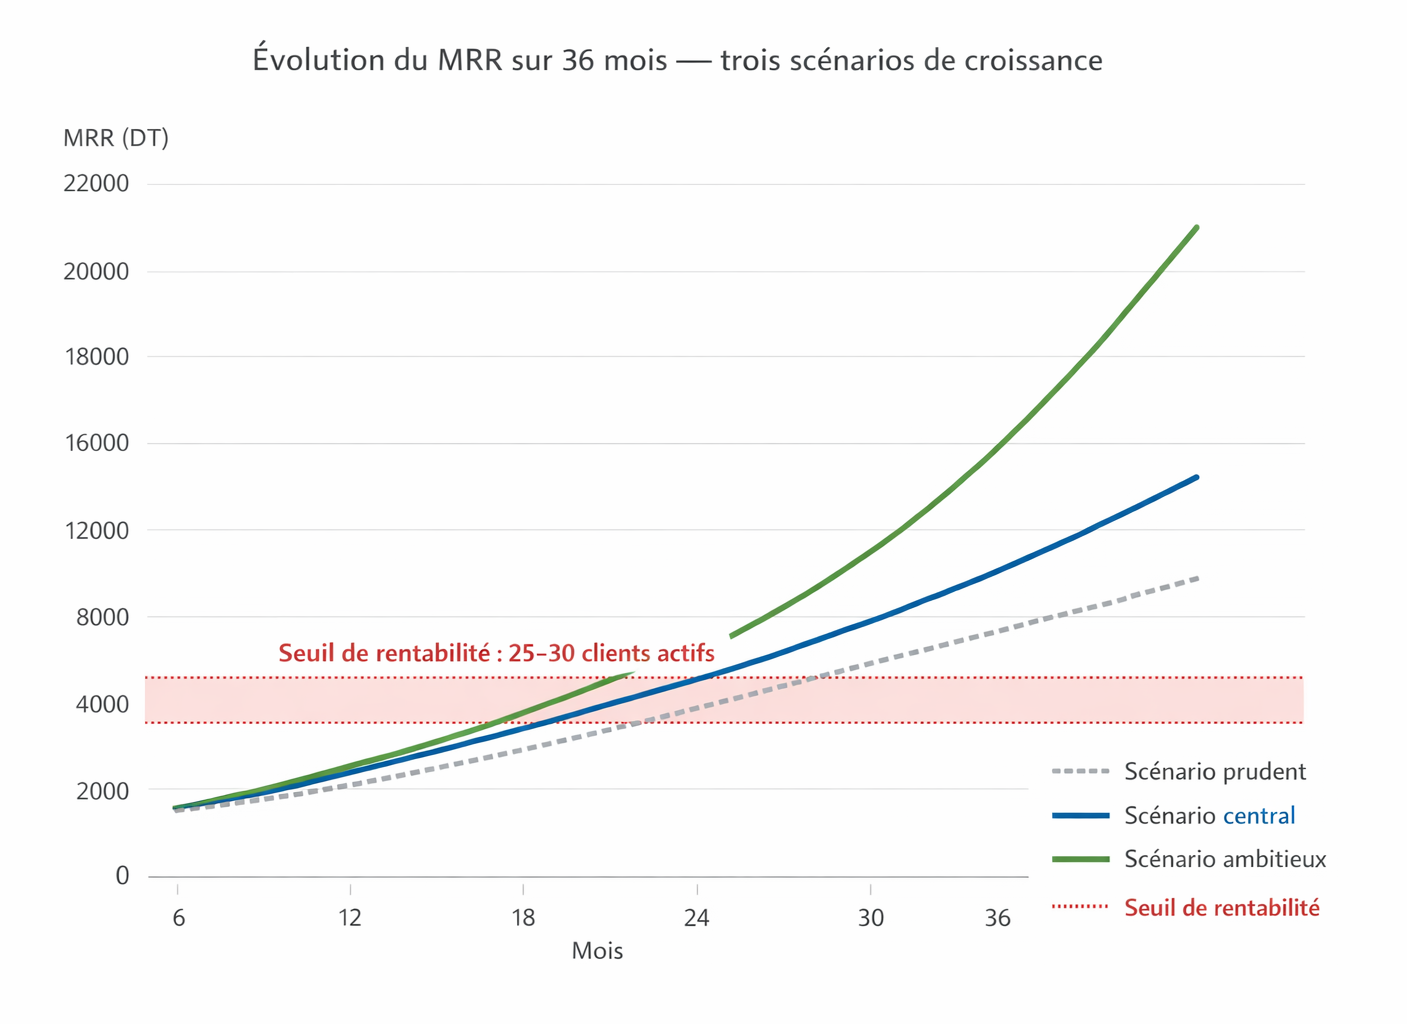
\includegraphics[width=\textwidth]{figures/mrr_evolution_36mois.png}
\caption{Évolution du MRR sur 36 mois --- trois scénarios de croissance}
\label{fig:mrr_evolution}
\end{figure}

%%%%%%%%%%%%%%%%%%%%%%%%%%%%%%%%%%%%%%%%%%%%%%%%%%%%%%%%%%%%%%%%%%%%%%%%%%%
\subsection{Lecture stratégique des scénarios}
\label{section3.10.2}
%%%%%%%%%%%%%%%%%%%%%%%%%%%%%%%%%%%%%%%%%%%%%%%%%%%%%%%%%%%%%%%%%%%%%%%%%%%

Le \textbf{scénario prudent} (20 clients en an 1) correspond à un rythme d'acquisition de 1 à 2 nouveaux clients par mois, avec un churn non encore maîtrisé. La rentabilité n'est atteinte qu'en début d'année 3. Ce scénario reste viable à condition de maintenir les charges fixes sous contrôle strict et de ne pas recruter avant que le MRR couvre les coûts fixes. Il représente le plancher de survie --- le scénario dans lequel le projet ne meurt pas, mais ne décolle pas non plus.

Le \textbf{scénario central} (40 clients en an 1, 100 en an 3) est le scénario de référence. Il suppose un rythme de 3 à 4 nouveaux clients par mois, cohérent avec un budget Meta Ads de 500 DT/mois et un taux de conversion free-to-paid de 15~\%. La rentabilité est atteinte au troisième trimestre de l'année 2 et le MRR dépasse 12\,000 DT en fin d'année 3 --- un niveau qui permet le réinvestissement en produit et en équipe.

Le \textbf{scénario ambitieux} (65 clients en an 1) suppose une diffusion accélérée par le bouche-à-oreille dans le réseau des e-commerçants ou par un partenariat de distribution avec une plateforme locale. La rentabilité est atteinte dès le quatrième trimestre de l'année 1. Ce scénario n'est pas irréaliste : il requiert un taux de recommandation élevé et un NPS supérieur à 50, deux conditions atteignables si la qualité dialectale et la fiabilité du service sont au rendez-vous.

\begin{tcolorbox}[colback=gray!8, colframe=gray!50, title=\textbf{Seuil critique opérationnel}, fonttitle=\bfseries]
Dans tous les scénarios, le seuil de rentabilité mensuelle est atteint à partir de \textbf{25 à 30 clients actifs}, soit un MRR de 3\,000 à 3\,600 DT. Ce chiffre est la milestone absolue du projet : en deçà, Vocallia consomme de la trésorerie ; au-delà, elle génère du profit réinvestissable. Il justifie rétrospectivement chaque décision de la chaîne stratégique : la concentration sur le Segment A (cycle de vente court), le pilote gratuit (accélérateur d'activation), le modèle PLG (coût d'acquisition minimal), le pricing à 79 DT (zone de confort validée). Toutes ces décisions sont calibrées pour atteindre 25 clients actifs dans les 12 premiers mois --- un objectif que même le scénario prudent atteint avant le mois 18.
\end{tcolorbox}

%%%%%%%%%%%%%%%%%%%%%%%%%%%%%%%%%%%%%%%%%%%%%%%%%%%%%%%%%%%%%%%%%%%%%%%%%%%
\section{Facteurs d'adoption et obstacles commerciaux}
\label{section3.11}
%%%%%%%%%%%%%%%%%%%%%%%%%%%%%%%%%%%%%%%%%%%%%%%%%%%%%%%%%%%%%%%%%%%%%%%%%%%

L'adoption d'une solution IA vocale par des PME e-commerce tunisiennes ne suit pas une logique linéaire. Elle s'inscrit dans la courbe de diffusion des innovations de Rogers (1962) : innovateurs (2,5~\%), adopteurs précoces (13,5~\%), majorité précoce (34~\%), majorité tardive (34~\%), retardataires (16~\%). La stratégie de Vocallia vise d'abord les adopteurs précoces --- profil Segment A --- avant de traverser le \og{}gouffre\fg{} vers la majorité précoce. Le tableau suivant identifie chaque facteur d'adoption ou de résistance et y associe la réponse stratégique déployée dans les sections précédentes.

\begin{table}[H]
\centering
\caption{Facteurs d'adoption et obstacles commerciaux --- Vocallia}
\vspace{4pt}
\begin{tabularx}{\textwidth}{|>{\raggedright\arraybackslash}p{3cm}|>{\raggedright\arraybackslash}p{1.8cm}|>{\raggedright\arraybackslash}p{1.5cm}|>{\raggedright\arraybackslash}X|}
\hline
\textbf{Facteur} & \textbf{Nature} & \textbf{Impact} & \textbf{Réponse stratégique} \\
\hline
Autofinancement visible dès le 1er mois & Accélérateur & Élevé & Formule de valeur chiffrée intégrée au dashboard, calculée sur données réelles \\
\hline
Naturalité du dialecte tunisien & Accélérateur & Très élevé & Démonstration audio sur appel réel avant tout engagement commercial \\
\hline
Pilote sans engagement financier & Accélérateur & Élevé & 50 appels gratuits : suppression totale du risque perçu à l'entrée \\
\hline
Références clients locales publiées & Accélérateur & Moyen & Recruter 3--5 ambassadeurs pilotes dès le lancement, avec témoignages vidéo \\
\hline
Résistance au changement (appel humain habituel) & Frein & Élevé & Démonstration comparative IA vs appel humain sur même script, métriques à l'appui \\
\hline
Crainte que l'IA soit mal perçue par les clients finaux & Frein & Moyen & Transparence dans les scripts + statistiques de satisfaction client post-appel \\
\hline
Sensibilité prix des PME tunisiennes & Frein & Élevé & Plan Starter à 79 DT aligné sur la zone de confort terrain. Pilote gratuit. \\
\hline
Absence de référence au lancement & Frein & Moyen & Partenariat 5 marchands pilotes avec études de cas publiées sur le site \\
\hline
Dépendance à la qualité du dialecte & Risque & Élevé & Amélioration continue des scripts, fine-tuning des prompts, boucle de feedback client \\
\hline
\end{tabularx}
\end{table}

%%%%%%%%%%%%%%%%%%%%%%%%%%%%%%%%%%%%%%%%%%%%%%%%%%%%%%%%%%%%%%%%%%%%%%%%%%%
\section{Conclusion}
\label{conclusion3}
%%%%%%%%%%%%%%%%%%%%%%%%%%%%%%%%%%%%%%%%%%%%%%%%%%%%%%%%%%%%%%%%%%%%%%%%%%%

Ce chapitre a construit la viabilité commerciale de Vocallia selon une chaîne stratégique où chaque décision découle de la précédente et en renforce la suivante. Quatre conclusions s'imposent.

\textbf{Le modèle est monétisable maintenant.} Le Segment A --- e-commerçants tunisiens à fort volume COD --- subit une douleur quotidienne et coûteuse à laquelle aucune solution locale ne répond. Le positionnement, la proposition de valeur et le pricing ont été calibrés sur ce segment. L'abonnement Starter à 79 DT génère une marge brute de 73,4~\% côté fournisseur et s'autofinance côté client, et 63,6~\% des répondants terrain acceptent un prix dans cette zone. La monétisation ne dépend pas d'une éducation du marché : le besoin est structurel et le client le sait.

\textbf{Le modèle scale.} Une marge brute pondérée supérieure à 65~\%, une structure de coûts dominée par les variables, et un modèle hybride abonnement/usage qui aligne revenus et valeur créée. Chaque client supplémentaire améliore la marge sans augmenter les coûts fixes. Le ratio LTV:CAC entre 10:1 et 16:1 --- avec un CAC payback inférieur à 2 mois et un coût d'acquisition 8 à 40 fois inférieur aux benchmarks sectoriels --- confirme que le modèle d'acquisition est soutenable bien au-delà du marché tunisien initial.

\textbf{Le modèle est défendable.} La barrière linguistique (dialecte tunisien natif + code-switching) offre une fenêtre d'avance de 18 à 36 mois. Chaque client actif enrichit le corpus de données d'appels locales, chaque mois d'usage augmente les coûts de migration vers un concurrent, et le réseau de témoignages se densifie. La défendabilité n'est pas statique : elle se renforce avec le temps.

\textbf{L'exécution est réaliste.} Le seuil de rentabilité opérationnelle --- 25 à 30 clients --- est atteignable dans les 12 à 18 premiers mois avec le modèle PLG déployé. Même dans le scénario le plus conservateur, le projet atteint l'équilibre en début d'année 3. Dans le scénario central, le MRR dépasse 12\,000 DT en fin d'année 3, ouvrant la voie au réinvestissement en produit et en expansion géographique.

\begin{quote}
\textit{Le chapitre suivant examinera la viabilité technique de Vocallia : architecture vocale, stack technologique, flux d'appel, latence, gestion des cas limites, besoins fonctionnels et non-fonctionnels, et ressources nécessaires au déploiement opérationnel de la solution.}
\end{quote}
%%%%%%%%%%%%%%%%%%%%%%%%%%%%%%%%%%%%%%%%%%%%%%%%%%%%%%%%%%%%%%%%%%%%%%%%%%%
\chapter{Étude de la viabilité technique}
\label{Chapitre_4}
%%%%%%%%%%%%%%%%%%%%%%%%%%%%%%%%%%%%%%%%%%%%%%%%%%%%%%%%%%%%%%%%%%%%%%%%%%%
\section{Introduction}
\label{sec:intro_chap4}
%%%%%%%%%%%%%%%%%%%%%%%%%%%%%%%%%%%%%%%%%%%%%%%%%%%%%%%%%%%%%%%%%%%%%%%%%%%

Les chapitres précédents ont établi que Vocallia répond à un besoin structurel, sur un marché captif, selon un modèle économique scalable et défendable. Ces conclusions ne valent toutefois qu'à une condition sine qua non~: que la solution soit techniquement réalisable, opérationnellement fiable et industriellement déployable avec les technologies disponibles aujourd'hui. Une infrastructure conversationnelle vocale en dialecte tunisien, capable de soutenir des appels sortants en temps quasi réel, avec une qualité dialectale suffisante pour ne pas dégrader l'expérience client, ne se résume pas à un assemblage d'API~: elle exige une orchestration rigoureuse, une gestion fine de la latence, une résilience face aux défaillances de fournisseurs tiers et une conformité réglementaire intégrée dès la conception.

Ce chapitre démontre, étape par étape, que cette exigence peut être tenue. L'analyse procède par couches successives~: des exigences fonctionnelles et non fonctionnelles à l'architecture globale, puis aux modules logiques, au pipeline conversationnel et à l'orchestration IA, jusqu'aux dimensions transverses que sont la sécurité, la scalabilité, l'observabilité et le déploiement. Chaque décision technique est justifiée par les objectifs produit définis aux chapitres~2 et~3~: maîtrise du darija, soutenabilité du coût par appel, fiabilité opérationnelle, traçabilité complète et conformité INPDP. Le chapitre se conclut par l'examen lucide des limites techniques résiduelles et des mécanismes de mitigation associés. L'objectif n'est pas de décrire une stack — c'est de prouver que l'architecture choisie rend Vocallia non seulement faisable, mais durablement opérable et évolutive.

%%%%%%%%%%%%%%%%%%%%%%%%%%%%%%%%%%%%%%%%%%%%%%%%%%%%%%%%%%%%%%%%%%%%%%%%%%%
\section{Exigences et contraintes techniques}
\label{sec:exigences_techniques}
%%%%%%%%%%%%%%%%%%%%%%%%%%%%%%%%%%%%%%%%%%%%%%%%%%%%%%%%%%%%%%%%%%%%%%%%%%%

La définition rigoureuse des exigences techniques est la condition initiale de toute architecture cohérente. Trois familles d'exigences structurent la conception de Vocallia~: les exigences fonctionnelles, qui décrivent ce que le système doit faire~; les exigences non fonctionnelles, qui définissent comment il doit le faire~; et les contraintes spécifiques au projet, qui bornent l'espace des solutions techniquement et réglementairement acceptables.

\subsection{Exigences fonctionnelles}
\label{subsec:exigences_fonctionnelles}

Les exigences fonctionnelles découlent directement du parcours client défini en section~3.7 et de la promesse produit formulée en section~3.2. Elles couvrent six familles de capacités. La première concerne la \textbf{gestion des organisations et des utilisateurs}~: création de comptes marchands, hiérarchie de rôles (administrateur, opérateur, lecture seule), invitation de collaborateurs, gestion d'équipes par organisation. La deuxième porte sur la \textbf{gestion des campagnes et des appels}~: réception des commandes via webhook, planification d'appels sortants, paramétrage de scripts par campagne, gestion des relances, file d'attente avec priorisation. La troisième regroupe les \textbf{capacités conversationnelles}~: reconnaissance vocale en darija avec code-switching arabe/français, compréhension d'intentions (confirmation, annulation, demande d'information, indisponibilité), génération de réponses naturelles, synthèse vocale en dialecte tunisien. La quatrième couvre les \textbf{intégrations métier}~: connecteurs natifs avec les principales plateformes e-commerce (Shopify, WooCommerce), API REST pour intégrations personnalisées, webhooks de remontée de statut. La cinquième concerne le \textbf{tableau de bord et le reporting}~: visualisation des appels en quasi-temps réel, métriques agrégées (taux de confirmation, taux de joignabilité, durée moyenne), export de transcriptions, rapports mensuels automatisés. La sixième porte sur l'\textbf{administration et l'observabilité}~: gestion des secrets API, supervision des intégrations, journaux d'audit, alerting opérationnel.

\subsection{Exigences non fonctionnelles}
\label{subsec:exigences_non_fonctionnelles}

Les exigences non fonctionnelles définissent les seuils de qualité opérationnelle que l'architecture vise à garantir. Elles sont synthétisées dans le tableau~\ref{tab:exigences_nf}~: chacune est posée comme un objectif technique réaliste, à atteindre par les choix d'architecture détaillés dans la suite du chapitre.

\begin{table}[H]
\centering
\caption{Exigences non fonctionnelles — cibles techniques de Vocallia}
\label{tab:exigences_nf}
\begin{tabular}{|p{4cm}|p{5cm}|p{5cm}|}
\hline
\textbf{Dimension} & \textbf{Cible technique} & \textbf{Justification produit} \\
\hline
Latence conversationnelle & Délai de réponse de bout en bout visé autour d'une seconde par tour de parole & Seuil au-delà duquel l'échange est perçu comme artificiel et dégrade l'expérience client \\
\hline
Disponibilité du service & Cible élevée, compatible avec un usage e-commerce continu & Limiter au strict minimum les fenêtres d'indisponibilité affectant la confirmation des commandes \\
\hline
Scalabilité horizontale & Capacité à absorber la croissance du volume d'appels sans refonte & Permet d'accompagner la trajectoire commerciale projetée jusqu'au scénario ambitieux d'année~3 \\
\hline
Sécurité des données & Chiffrement en transit (TLS) et au repos sur les données sensibles & Conformité INPDP et standards de sécurité B2B exigés par les clients institutionnels \\
\hline
Multi-tenancy & Isolation logique stricte entre organisations & Indispensable pour un SaaS B2B servant plusieurs marchands potentiellement concurrents \\
\hline
Observabilité & Couverture logs, métriques et traces & Diagnostic rapide des incidents et amélioration continue des performances dialectales \\
\hline
Évolutivité fonctionnelle & Architecture modulaire à couplage faible & Permet l'ajout de nouveaux cas d'usage (relance, prise de RDV) sans refonte \\
\hline
\end{tabular}
\end{table}

\subsection{Contraintes spécifiques au projet}
\label{subsec:contraintes_projet}

Au-delà des exigences génériques d'un SaaS B2B, Vocallia opère sous quatre contraintes spécifiques qui ont guidé l'ensemble des choix architecturaux. La \textbf{contrainte linguistique} est la plus structurante~: aucun fournisseur d'API global ne maîtrise nativement le darija avec son code-switching arabe/français caractéristique. L'architecture doit donc intégrer des couches d'adaptation propriétaires (ingénierie de prompts, normalisation phonétique, post-traitement) sur des modèles génériques. La \textbf{contrainte réglementaire} impose une conformité ab initio à la loi n°2004-63 et aux exigences de l'INPDP~: consentement explicite, durée de rétention bornée à 30~jours, droit de suppression, traçabilité des traitements. La \textbf{contrainte économique} découle directement du modèle de tarification présenté en section~3.8~: le coût variable par appel de deux minutes, estimé à environ 0{,}27~DT, doit rester compatible avec un prix d'entrée du palier Starter de 0{,}79~DT par appel, afin de préserver une marge brute soutenable de l'ordre de 65~\% sur ce palier. La \textbf{contrainte de dépendance fournisseurs}, enfin, impose une architecture multi-fournisseurs ouvrant la possibilité de substituer un provider STT, LLM, TTS ou téléphonie en cas de hausse tarifaire ou d'interruption — exigence directement issue de l'analyse SWOT en section~3.4.

\begin{quote}
\textbf{Lecture stratégique des exigences.} Les quatre contraintes spécifiques agissent comme un \emph{filtre architectural}~: chaque décision technique du présent chapitre est évaluée à l'aune de sa capacité à respecter simultanément la cible de latence, la soutenabilité économique du plan Starter, la conformité INPDP et la substituabilité des fournisseurs. Une solution qui satisferait trois de ces quatre critères mais en échouerait un seul est rejetée. Cette discipline distingue une architecture viable d'un assemblage opportuniste de technologies.
\end{quote}

%%%%%%%%%%%%%%%%%%%%%%%%%%%%%%%%%%%%%%%%%%%%%%%%%%%%%%%%%%%%%%%%%%%%%%%%%%%
\section{Architecture technique globale}
\label{sec:architecture_globale}
%%%%%%%%%%%%%%%%%%%%%%%%%%%%%%%%%%%%%%%%%%%%%%%%%%%%%%%%%%%%%%%%%%%%%%%%%%%

L'architecture globale de Vocallia adopte un modèle en couches à responsabilités séparées, conçu pour maximiser la modularité, la testabilité et la substituabilité des composants externes. Cinq couches structurent le système, organisées de l'interface utilisateur jusqu'aux services tiers. La figure~\ref{fig:architecture_globale} en donne une vue synthétique~; les sous-sections qui suivent en commentent les choix les plus structurants.

\begin{figure}[H]
\centering
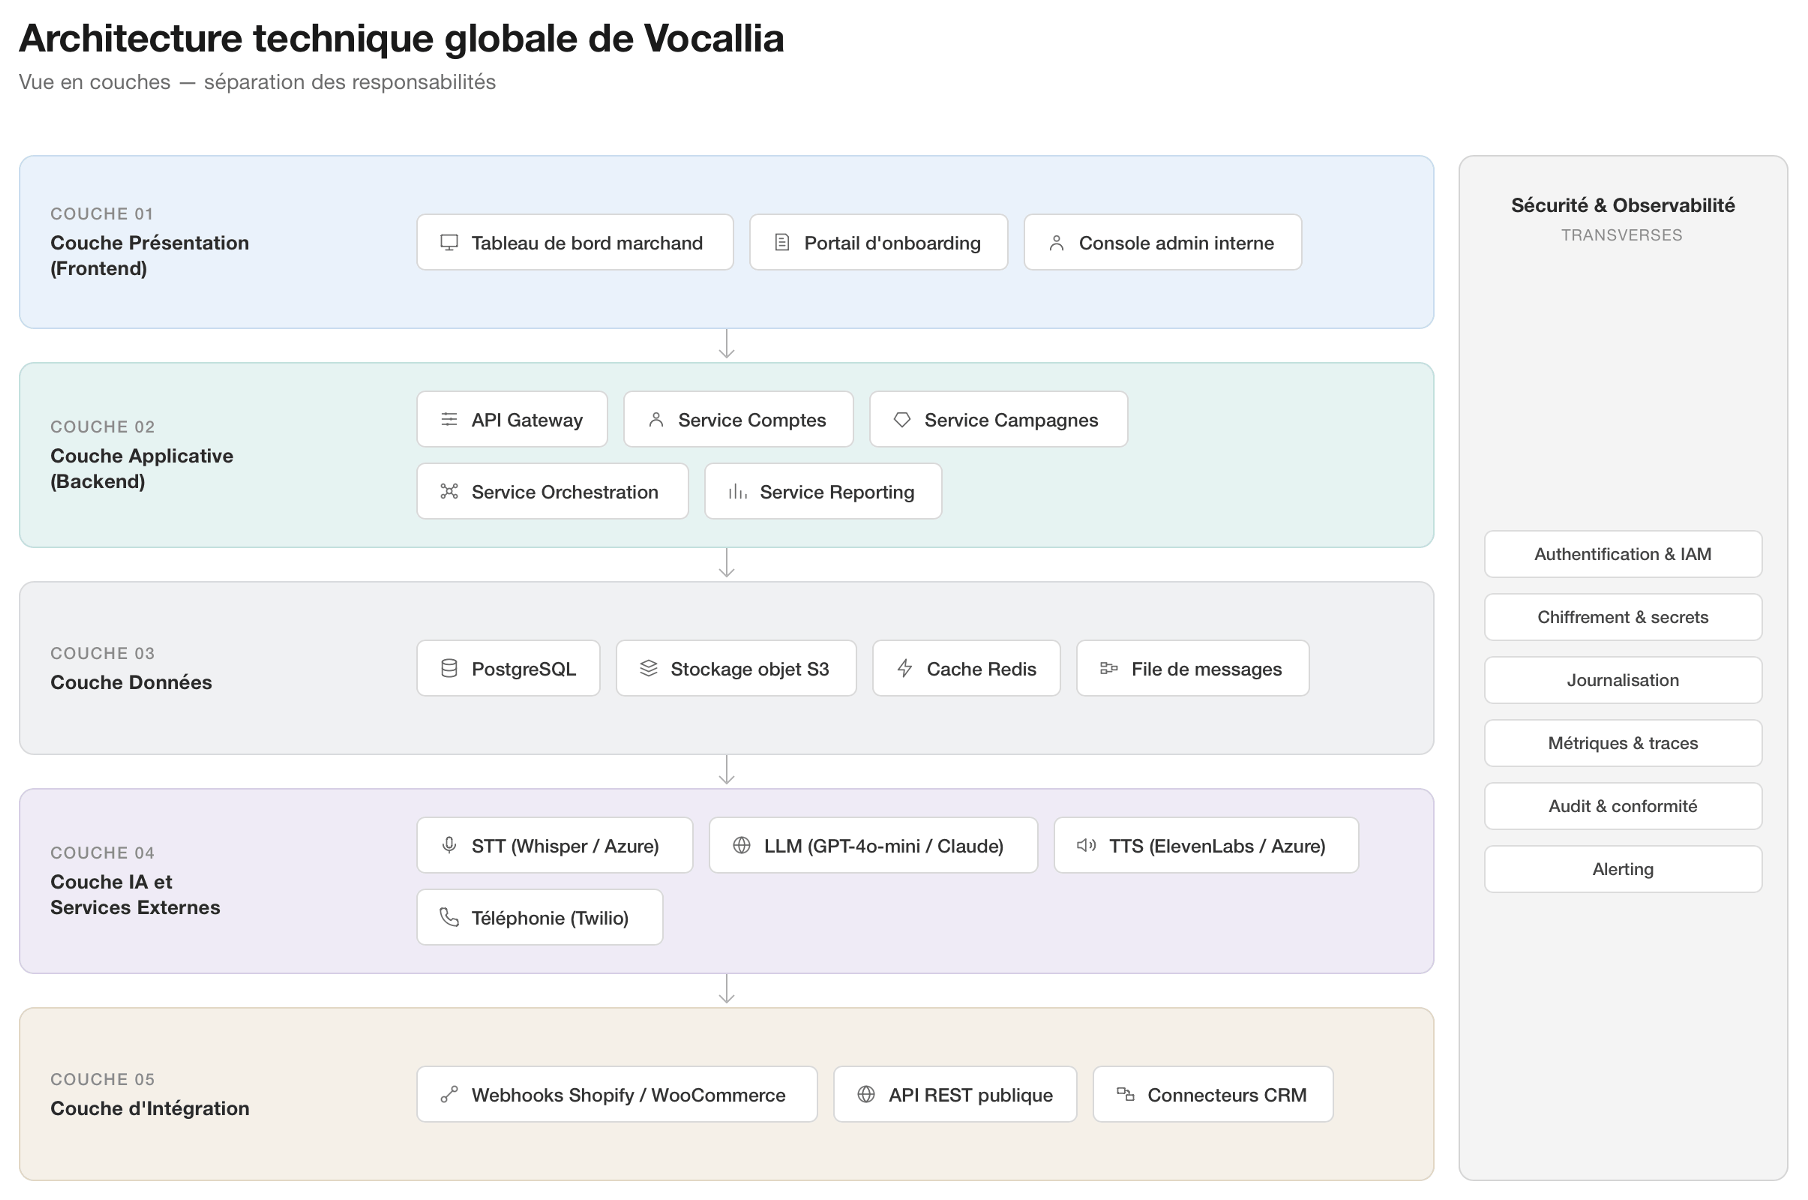
\includegraphics[width=\textwidth]{figures/architecture_globale_vocallia.png}
\caption{Architecture technique globale de Vocallia — vue en couches}
\label{fig:architecture_globale}
\end{figure}

\subsection{Couche présentation}
\label{subsec:couche_frontend}

La couche présentation regroupe les interfaces utilisateur destinées aux marchands et aux administrateurs~: tableau de bord web responsive, portail d'onboarding self-service et console interne de supervision. Elle communique exclusivement avec la couche applicative via une API REST sécurisée. Aucune logique métier ne réside côté client, ce qui garantit la portabilité future vers des applications mobiles ou des intégrations partenaires sans duplication de code critique.

\subsection{Couche applicative}
\label{subsec:couche_backend}

La couche applicative constitue le cœur fonctionnel du système. Elle est structurée autour d'une \textbf{API Gateway} centralisée qui authentifie, autorise et route les requêtes vers une constellation de services métier découplés~: gestion des comptes, gestion des campagnes, planification des appels, orchestration conversationnelle, reporting. Cette modularité autorise un déploiement et un dimensionnement indépendants de chaque service en fonction de sa charge réelle — l'orchestration conversationnelle, plus exigeante, étant scalée différemment du reporting, qui reste à charge faible et stable.

\subsection{Couche données}
\label{subsec:couche_donnees}

La couche données combine plusieurs typologies de stockage, chacune adaptée à sa fonction. Une \textbf{base de données relationnelle} (PostgreSQL) héberge les données transactionnelles structurées~: comptes, organisations, campagnes, statuts d'appels, transcriptions textuelles. Un \textbf{stockage objet} (compatible S3) abrite les enregistrements audio bruts, soumis à une politique de rétention de 30~jours par défaut. Un \textbf{cache distribué} (Redis ou équivalent) accélère les opérations à forte fréquence~: gestion de sessions, files d'attente, paramètres de configuration. Une \textbf{file de messages} (RabbitMQ, NATS ou équivalent) découple les déclencheurs d'appels du moteur d'exécution, permettant l'absorption de pics de charge sans dégradation perceptible côté marchand.

\subsection{Couche IA et services externes}
\label{subsec:couche_ia_externes}

La couche IA encapsule les appels aux fournisseurs externes derrière une interface d'abstraction unique. Trois familles de services sont mobilisées~: les \textbf{moteurs de reconnaissance vocale} (Whisper d'OpenAI à titre principal, avec adaptateurs vers Azure Speech ou Google Speech-to-Text en repli), les \textbf{modèles de langage} (GPT-4o-mini comme moteur de référence, avec adaptateurs vers Claude ou Mistral) et les \textbf{moteurs de synthèse vocale} (ElevenLabs en référence, avec Azure Neural TTS et Coqui en alternative). Cette abstraction est la traduction technique de l'exigence de substituabilité~: changer un fournisseur n'impacte qu'une classe d'adaptateur, jamais le code applicatif.

\subsection{Couche d'intégration}
\label{subsec:couche_integration}

La couche d'intégration assure les échanges bidirectionnels avec l'écosystème du marchand. Elle comprend des \textbf{connecteurs entrants} (webhooks Shopify, WooCommerce, API personnalisée pour systèmes propriétaires) qui déclenchent les campagnes d'appels, et des \textbf{connecteurs sortants} qui remontent les résultats vers le système du marchand (mise à jour de statut commande, alertes, synchronisation CRM). Le \textbf{module de téléphonie}, fondé sur Twilio à titre principal et conçu de manière abstraite pour permettre à terme un basculement vers un opérateur local, constitue l'interface critique vers le réseau téléphonique commuté.

\begin{quote}
\textbf{Cohérence architecture / objectifs produit.} Cette structure en cinq couches répond directement aux objectifs produit définis aux chapitres précédents. La séparation frontend / backend rend possible une distribution 100~\% digitale et un onboarding sans friction. La modularité des services applicatifs garantit l'évolutivité vers de nouveaux cas d'usage sans refonte. L'abstraction de la couche IA matérialise l'exigence de résilience multi-fournisseurs identifiée dans l'analyse SWOT. La couche d'intégration ouverte assure enfin la compatibilité avec l'écosystème e-commerce tunisien, condition d'adoption par des marchands déjà équipés.
\end{quote}

%%%%%%%%%%%%%%%%%%%%%%%%%%%%%%%%%%%%%%%%%%%%%%%%%%%%%%%%%%%%%%%%%%%%%%%%%%%
\section{Architecture logique et modulaire}
\label{sec:architecture_logique}
%%%%%%%%%%%%%%%%%%%%%%%%%%%%%%%%%%%%%%%%%%%%%%%%%%%%%%%%%%%%%%%%%%%%%%%%%%%

Là où l'architecture globale décrit la structure physique du système, l'architecture logique en décrit les responsabilités fonctionnelles. Vocallia est organisé en sept modules métier, conçus pour être faiblement couplés, indépendamment testables et évolutifs sans impact transversal. La figure~\ref{fig:architecture_logique} en propose la cartographie~; les sous-sections qui suivent ne reprennent pas exhaustivement chaque module, mais en précisent le rôle dans l'économie générale du système.

\begin{figure}[H]
\centering
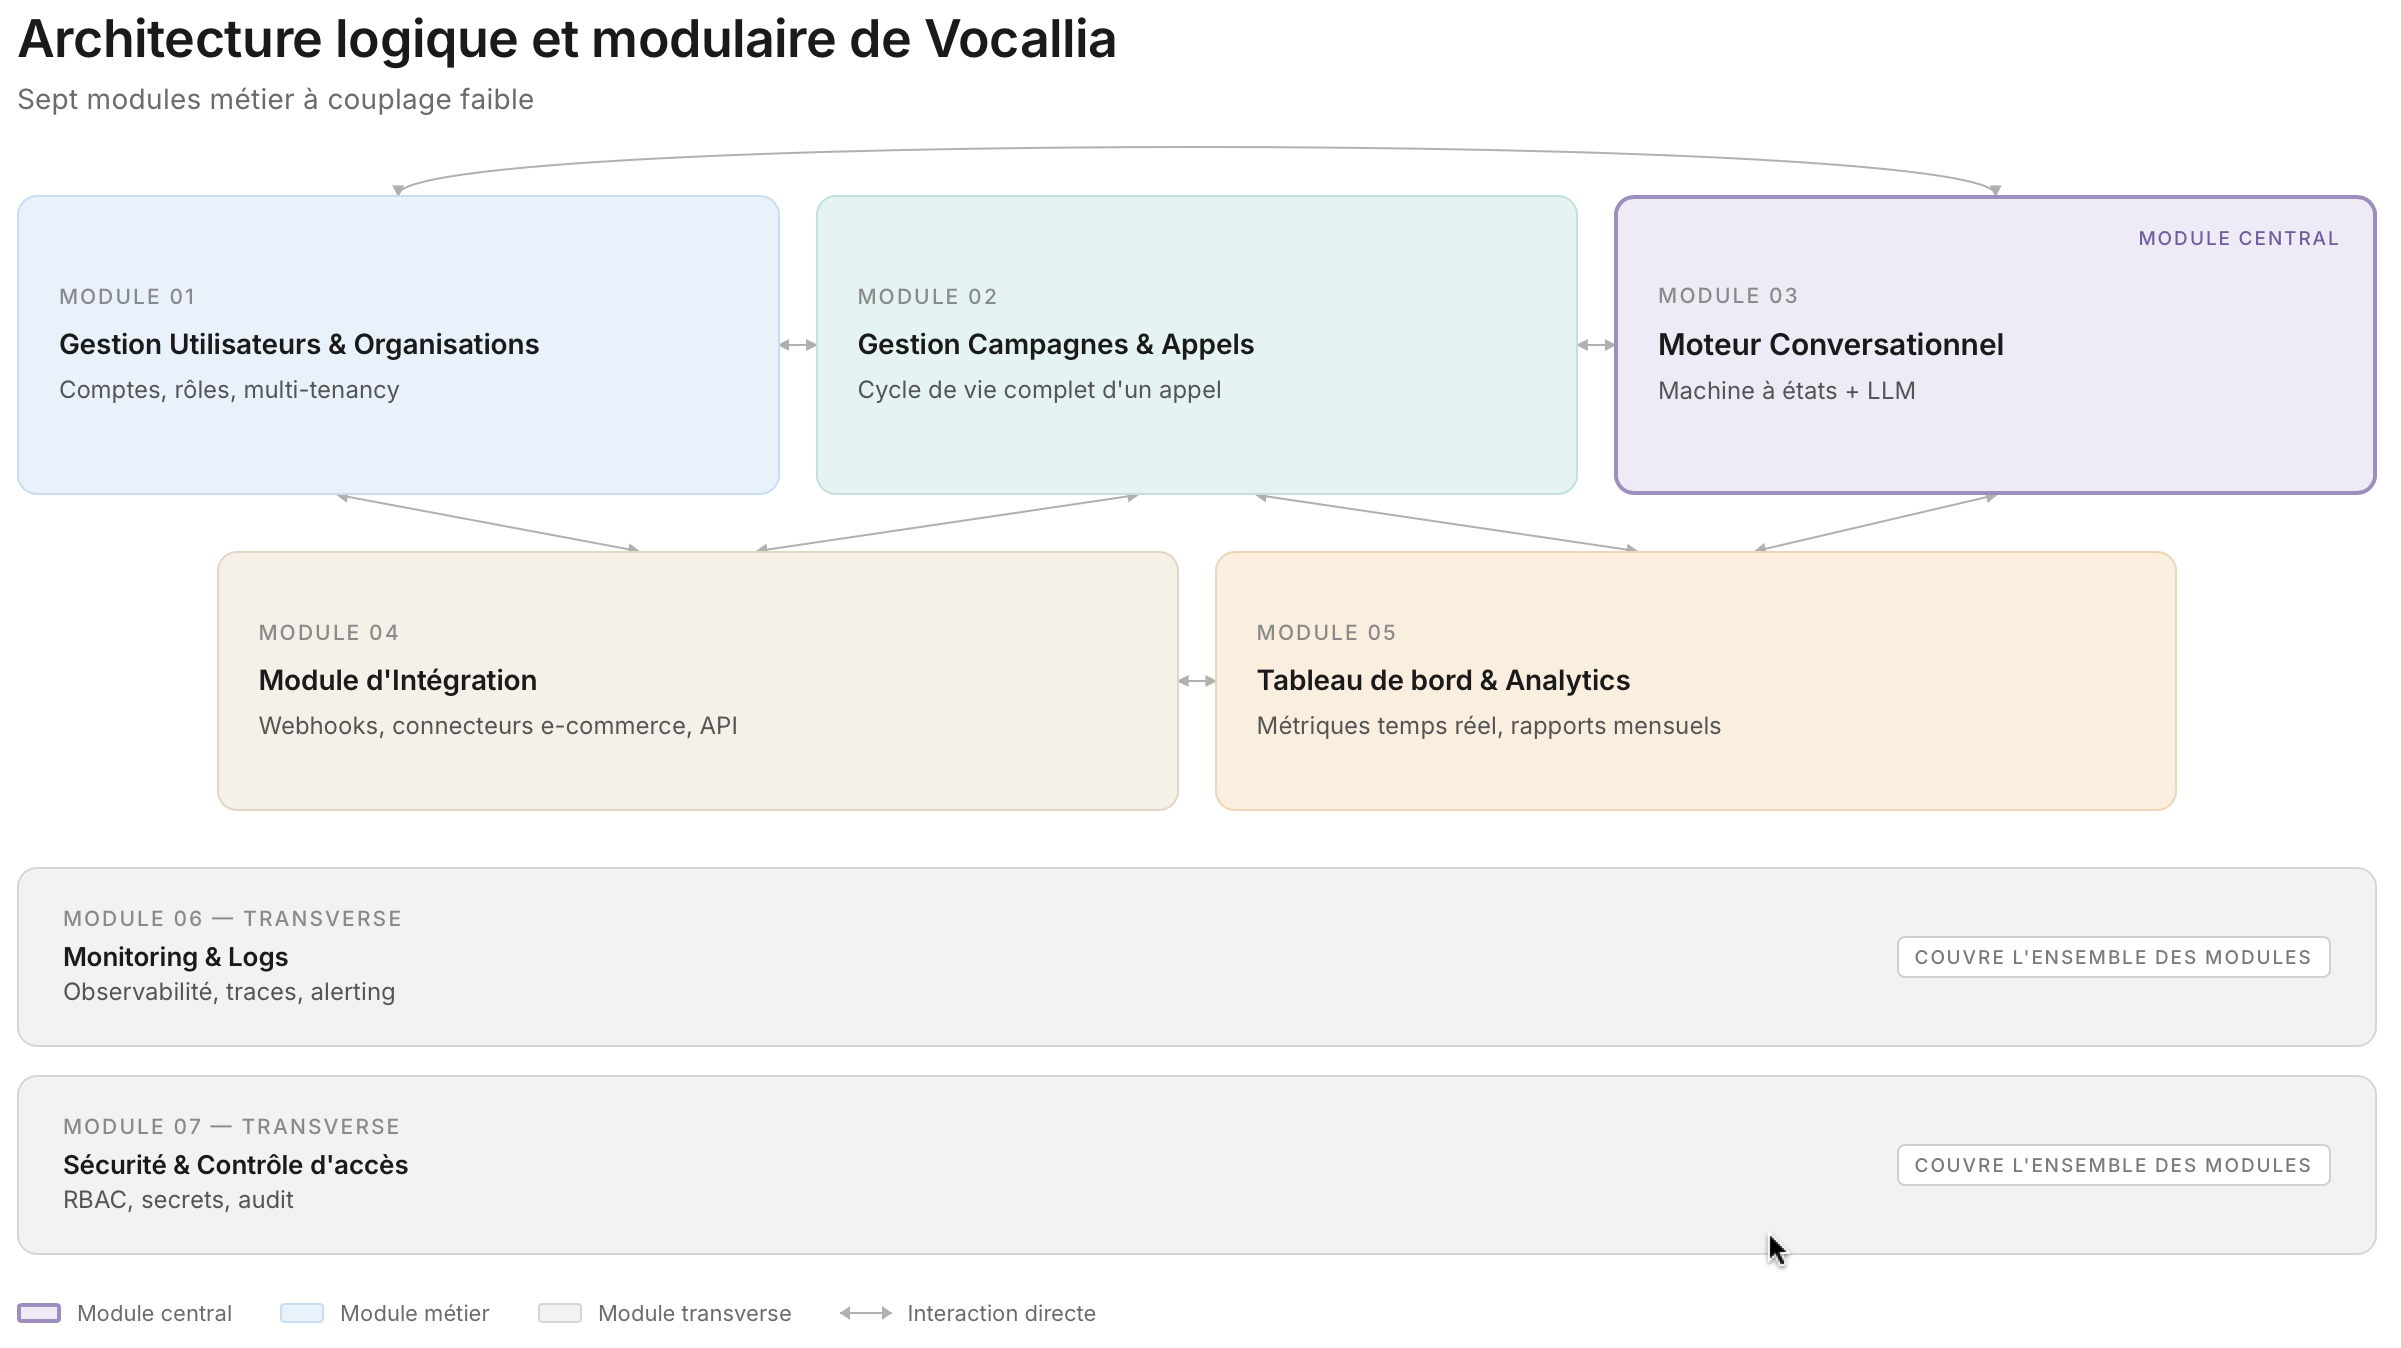
\includegraphics[width=\textwidth]{figures/architecture_logique_vocallia.png}
\caption{Architecture logique et modulaire de Vocallia — sept modules métier}
\label{fig:architecture_logique}
\end{figure}

\subsection{Modules d'identité et de campagnes}
\label{subsec:modules_id_campaigns}

Le module de \textbf{gestion des utilisateurs et des organisations} encapsule les opérations relatives à l'identité et constitue le socle de la multi-tenancy~: chaque ressource créée ailleurs est rattachée à une organisation, qui sert de frontière logique d'isolation pour toutes les requêtes ultérieures. Le module de \textbf{gestion des campagnes et des appels} orchestre le cycle de vie complet d'un appel — de la réception du webhook à la classification du résultat — et intègre la logique de relance automatique selon une stratégie d'intervalles configurable.

\subsection{Module moteur conversationnel}
\label{subsec:module_conversational}

Le moteur conversationnel est le composant le plus critique de l'architecture. Il implémente la machine à états du dialogue~: à chaque tour de parole, il reçoit la transcription du client, détermine l'intention, sélectionne la prochaine action et génère la réponse vocale. Sa structuration interne combine une couche déterministe (machine à états et règles métier) et une couche probabiliste (LLM pour l'interprétation des énoncés ambigus). Cette double nature, détaillée en section~\ref{sec:orchestration_ia}, garantit la prédictibilité du comportement sur les chemins critiques tout en préservant la souplesse conversationnelle attendue d'un agent vocal.

\subsection{Modules d'intégration, de tableau de bord et de monitoring}
\label{subsec:modules_horizontaux}

Le module d'\textbf{intégration} centralise les connexions aux systèmes externes du marchand~: gestion des webhooks entrants et sortants, transformations de format, gestion des erreurs (retry, dead-letter queue, alerting). Une bibliothèque de connecteurs natifs couvre les plateformes les plus courantes, tandis qu'une API générique permet l'intégration avec tout système exposant un endpoint REST. Le module de \textbf{tableau de bord et analytics} agrège, transforme et restitue les données opérationnelles aux marchands en quasi-temps réel, et alimente le rapport mensuel automatique présenté comme \emph{preuve physique} en section~3.6. Le module de \textbf{monitoring et logs}, transverse à l'ensemble du système, collecte logs, métriques et traces distribuées et déclenche les alertes pertinentes lorsque les seuils techniques sont franchis.

\subsection{Module de sécurité et contrôle d'accès}
\label{subsec:module_securite}

Le module de sécurité centralise les mécanismes transverses de protection~: gestion des tokens d'authentification, contrôle d'accès basé sur les rôles (RBAC), gestion des secrets API via un coffre-fort dédié, journalisation d'audit des actions sensibles et application des politiques de rétention. Sa conception isolée garantit que toute modification des règles de sécurité n'impacte qu'un point unique, réduisant le risque de configuration incohérente.

\begin{quote}
\textbf{Justification de la modularité.} Cette décomposition n'est pas un exercice théorique~: elle traduit en architecture la roadmap produit définie en section~3.6. L'extension future vers les cas d'usage de relance après abandon de panier, de prise de rendez-vous médicaux ou de qualification de leads ne nécessitera pas la création d'un nouveau système, mais l'instanciation de scénarios additionnels dans le moteur conversationnel et l'ajout de connecteurs dans le module d'intégration. Le socle technique est ainsi mutualisé entre tous les cas d'usage~: un seul corpus dialectal à enrichir, un seul tableau de bord à maintenir, une seule logique de sécurité à auditer. C'est cette mutualisation qui rend économiquement et techniquement crédible la transition d'un outil mono-usage vers une plateforme conversationnelle.
\end{quote}

%%%%%%%%%%%%%%%%%%%%%%%%%%%%%%%%%%%%%%%%%%%%%%%%%%%%%%%%%%%%%%%%%%%%%%%%%%%
\section{Pipeline conversationnel de Vocallia}
\label{sec:pipeline_conversationnel}
%%%%%%%%%%%%%%%%%%%%%%%%%%%%%%%%%%%%%%%%%%%%%%%%%%%%%%%%%%%%%%%%%%%%%%%%%%%

Le pipeline conversationnel est la séquence technique qui, à partir d'une commande reçue, produit un appel téléphonique automatisé en dialecte tunisien et restitue son résultat dans le système du marchand. Il constitue la chaîne de valeur technique de Vocallia~: chacun de ses maillons doit être individuellement performant, mais c'est l'orchestration de l'ensemble qui détermine la qualité perçue par le client final. La figure~\ref{fig:pipeline_conversationnel} en représente la séquence complète et le budget de latence cible. Les paragraphes qui suivent ne paraphrasent pas le schéma~: ils en explicitent les choix techniques les plus sensibles.

\begin{figure}[H]
\centering
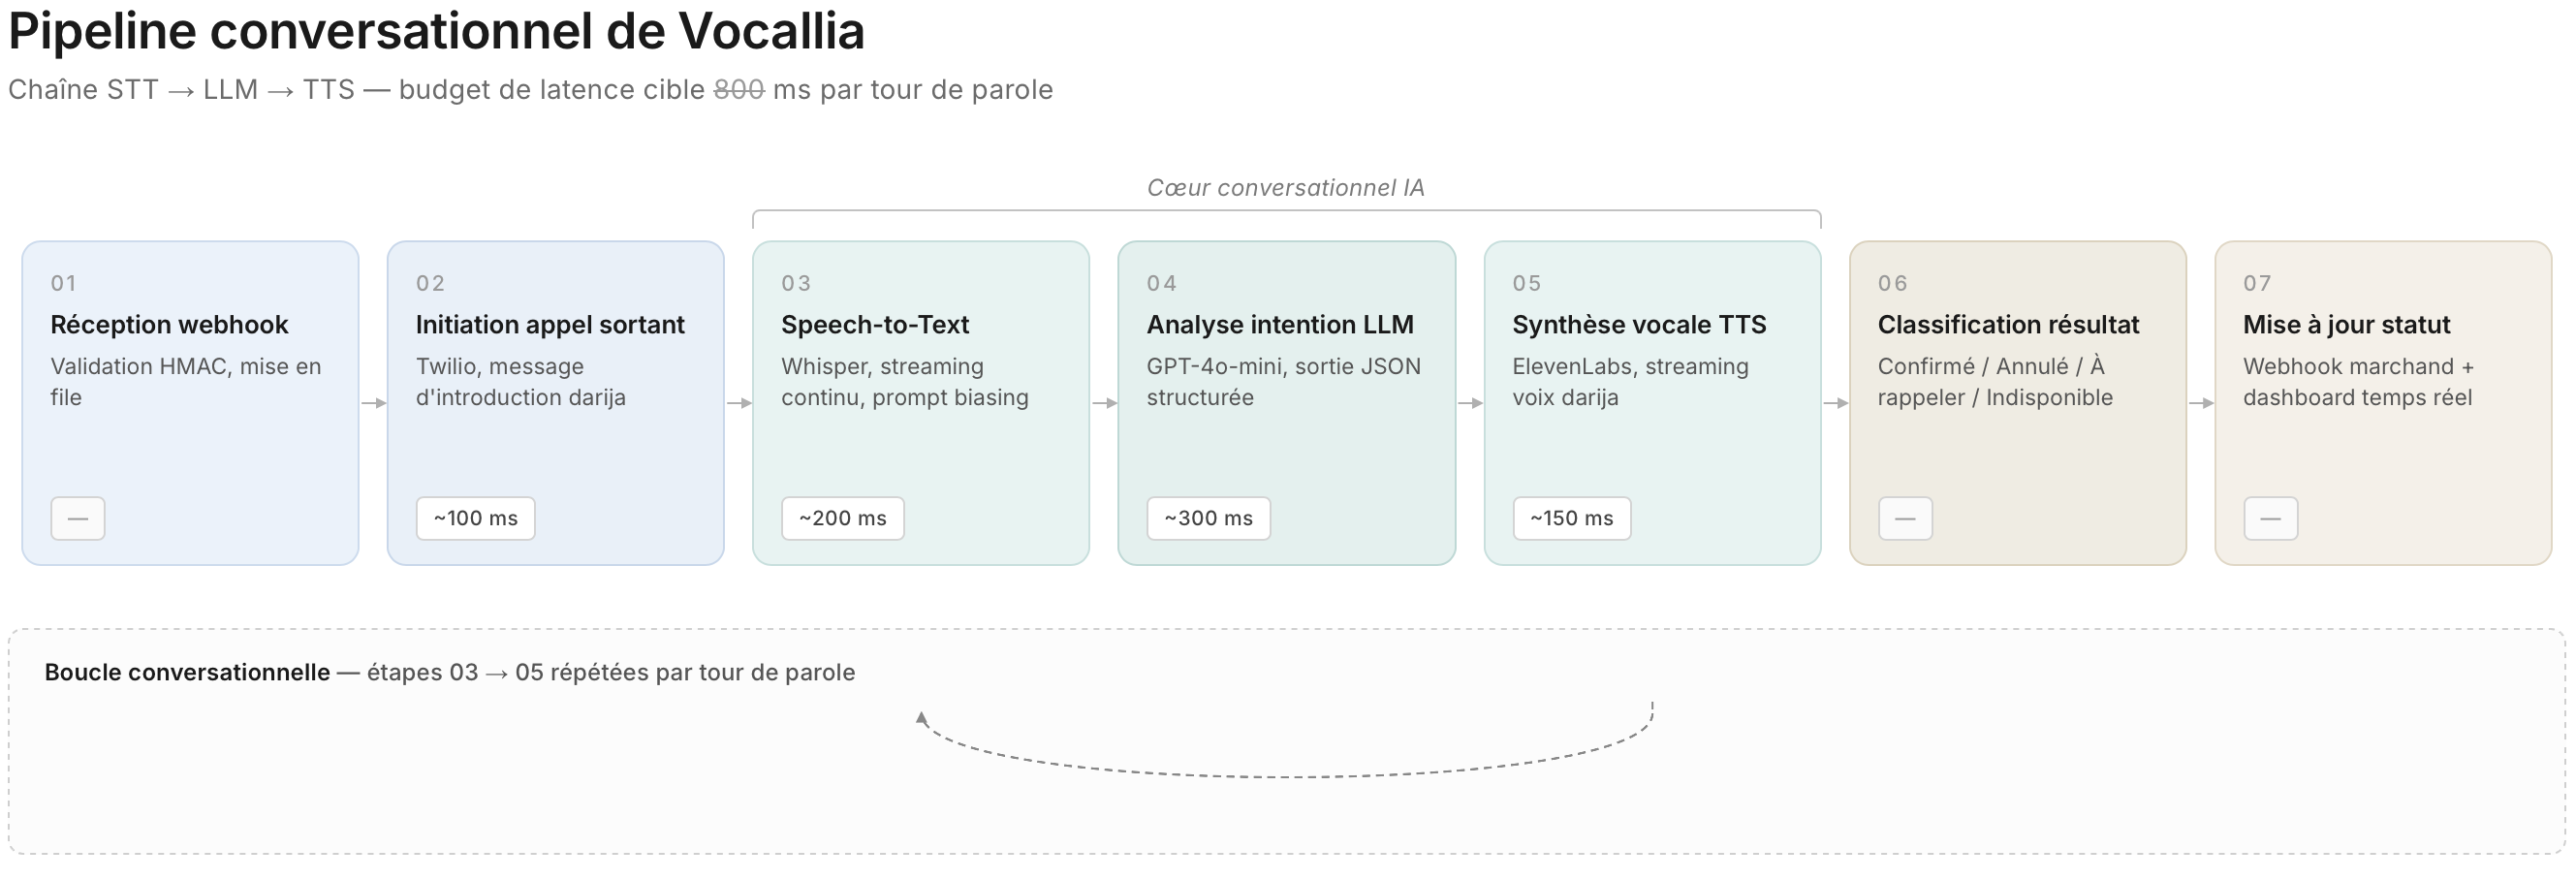
\includegraphics[width=\textwidth]{figures/pipeline_conversationnel_vocallia.png}
\caption{Pipeline conversationnel de Vocallia — chaîne STT $\to$ LLM $\to$ TTS et budget de latence}
\label{fig:pipeline_conversationnel}
\end{figure}

\subsection{Réception, déclenchement et message d'introduction}
\label{subsec:pipeline_amont}

À la réception d'une commande, un \textbf{webhook} est émis vers l'API de Vocallia. Le module d'intégration valide la signature (HMAC), authentifie l'organisation source, normalise les données et insère un job dans la file d'attente d'appels. Une réponse 200~OK est renvoyée immédiatement, garantissant que le webhook ne bloque pas le système du marchand même en cas de pic. Le worker d'exécution dépile ensuite le job, sélectionne la voix synthétique adaptée et déclenche l'appel sortant via l'API de téléphonie. Dès le décrochage, un \textbf{message d'introduction} en darija est diffusé pour signaler explicitement la nature automatisée de l'appel — exigence légale (loi n°2004-63) et bonne pratique conversationnelle qui réduit la confusion du destinataire.

\subsection{Reconnaissance vocale, analyse d'intention et synthèse vocale}
\label{subsec:pipeline_coeur}

Le flux audio du client est transmis au moteur STT en streaming continu. Whisper, principal moteur retenu, présente une couverture acceptable de l'arabe avec des limites documentées sur les sous-registres dialectaux les plus éloignés du standard. Vocallia compense ces limites par trois mécanismes complémentaires~: une \textbf{normalisation phonétique} en post-traitement, un \textbf{lexique de termes spécifiques} (noms de produits, vocabulaire e-commerce tunisien) injecté en \emph{prompt biasing} et un \textbf{score de confiance} évalué pour chaque énoncé. Lorsque la confiance descend sous un seuil défini, le moteur conversationnel déclenche une demande de clarification plutôt que d'inférer une intention non fiable.

Le texte transcrit est transmis au LLM avec un \textbf{prompt système} décrivant le contexte (commande, client, marchand), les intentions admises et les règles de réponse. Le modèle produit une sortie \textbf{structurée au format JSON} contenant l'intention détectée, les paramètres extraits, un score de confiance et une réponse textuelle. Cette structuration est délibérée~: elle permet d'appliquer des règles métier déterministes par-dessus la décision probabiliste du modèle, garantissant la prédictibilité sur les chemins critiques. La réponse est enfin transmise au TTS, configuré avec une voix adaptée au rendu darija. La synthèse fonctionne en \textbf{streaming bout en bout}~: l'audio est diffusé au client à mesure qu'il est généré, ce qui contracte significativement la latence perçue par rapport à une exécution séquentielle.

\subsection{Classification du résultat et restitution}
\label{subsec:pipeline_aval}

À l'issue de la conversation, le module de classification consolide les éléments collectés et attribue un résultat catégoriel à l'appel~: \emph{confirmé}, \emph{annulé}, \emph{à rappeler}, \emph{injoignable}, \emph{transféré à un humain} ou \emph{indéterminé}. Cette classification, qui combine intentions détectées et métadonnées techniques, est ensuite remontée en parallèle vers le \textbf{système du marchand} (mise à jour du statut de commande via webhook sortant) et vers le \textbf{tableau de bord} (mise à jour temps réel par WebSocket ou Server-Sent Events). La transcription complète et l'enregistrement audio sont stockés selon la politique de rétention configurée, et restent consultables par le marchand pour vérification ou ajustement des scripts.

\begin{quote}
\textbf{Budget de latence — analyse critique.} La cible globale d'environ une seconde par tour de parole est obtenue en allouant un budget par étape, indiqué sur la figure~\ref{fig:pipeline_conversationnel}. Cette répartition reste exigeante mais cohérente avec les performances publiées par les fournisseurs principaux. La marge de sécurité repose sur trois leviers~: le streaming bout en bout, la mise en cache des introductions vocales statiques et le dimensionnement adéquat de l'infrastructure d'inférence. Les tours de parole pour lesquels la latence dépasse la cible sont systématiquement journalisés~: ils alimentent le cycle d'amélioration continue plutôt que d'être traités comme des incidents isolés.
\end{quote}

%%%%%%%%%%%%%%%%%%%%%%%%%%%%%%%%%%%%%%%%%%%%%%%%%%%%%%%%%%%%%%%%%%%%%%%%%%%
\section{Orchestration IA et logique métier}
\label{sec:orchestration_ia}
%%%%%%%%%%%%%%%%%%%%%%%%%%%%%%%%%%%%%%%%%%%%%%%%%%%%%%%%%%%%%%%%%%%%%%%%%%%

L'orchestration IA est le maillon qui transforme un assemblage d'API en une expérience conversationnelle cohérente. Encapsulée dans le moteur conversationnel, elle conditionne l'ensemble de l'expérience produit~: une mauvaise orchestration produit une IA techniquement fonctionnelle mais commercialement inexploitable. La figure~\ref{fig:orchestration_ia} en synthétise les deux principes directeurs~: la coexistence d'une couche déterministe et d'une couche probabiliste, et un dispositif de fallback à trois niveaux.

\begin{figure}[H]
\centering
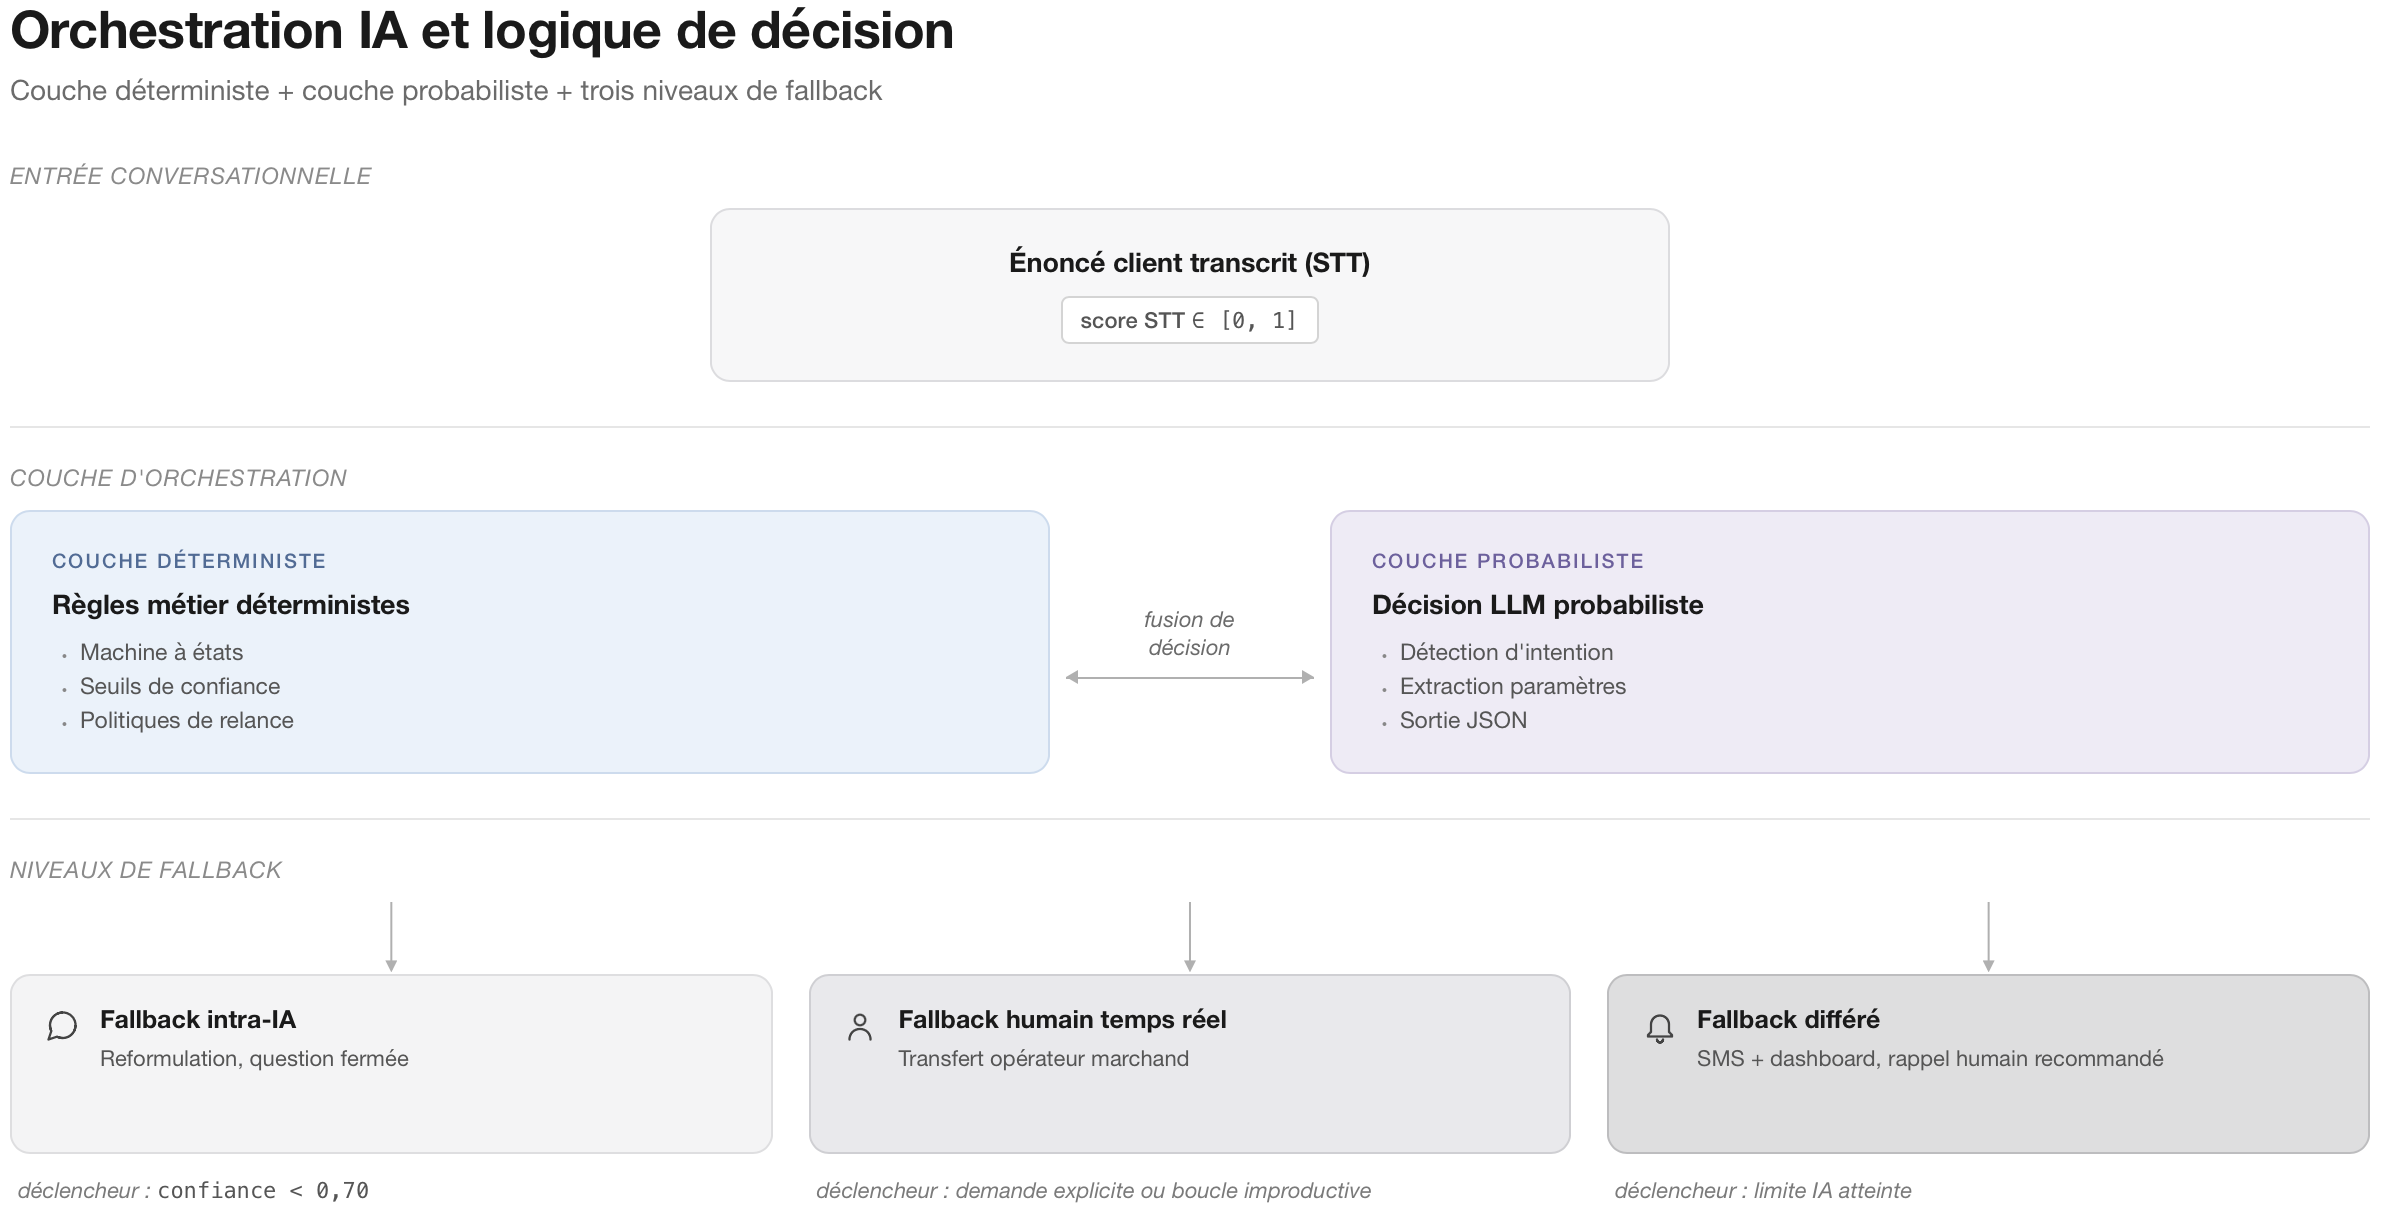
\includegraphics[width=\textwidth]{figures/orchestration_ia_vocallia.png}
\caption{Orchestration IA de Vocallia — couches de décision et niveaux de fallback}
\label{fig:orchestration_ia}
\end{figure}

\subsection{Coordination STT, LLM, TTS}
\label{subsec:orchestration_coord}

Les trois services ne sont pas appelés en série rigide mais coordonnés selon une logique adaptative. Le STT fonctionne en streaming continu, fournissant des transcriptions partielles à mesure que le client parle. Le moteur conversationnel détecte la fin d'énoncé (silence prolongé ou marqueur prosodique) et déclenche l'appel LLM. Pendant que le LLM raisonne, le moteur peut anticiper en envoyant au TTS le début d'une formule générique de transition (« \emph{matwasalsh, lehetna nchouf...} »), masquant ainsi efficacement la latence perçue. Cette technique de \emph{filler conversationnel}, courante dans les systèmes vocaux avancés, ramène la latence ressentie en deçà du seuil de gêne même lorsque la latence absolue dépasse temporairement la cible.

\subsection{Logique de décision et règles métier}
\label{subsec:orchestration_decision}

Le moteur conversationnel n'est pas un simple proxy vers le LLM. Il superpose à la décision probabiliste du modèle une couche de \textbf{règles métier déterministes} qui garantissent la prédictibilité du comportement sur les chemins critiques. À titre d'illustration~: si le LLM détecte une intention de \emph{confirmation} avec un score de confiance élevé et que le contenu de la commande lu au client a été acquitté, la commande est marquée confirmée sans nouvelle interrogation~; si le score est faible, une question de clarification fermée (« \emph{tetbet ?} » — « vous confirmez~? ») est déclenchée. Cette double couche — probabiliste pour la flexibilité linguistique, déterministe pour la rigueur métier — est la condition d'un système simultanément naturel et fiable.

\subsection{Mécanismes de fallback et escalade humaine}
\label{subsec:orchestration_fallback}

L'IA n'est pas conçue pour traiter tous les cas, mais pour traiter \emph{les cas pour lesquels elle est fiable} et pour reconnaître et escalader les autres. Trois niveaux de fallback sont implémentés. Le \textbf{premier niveau} déclenche une demande de clarification ou une reformulation lorsque la confiance STT ou LLM est trop faible. Le \textbf{deuxième niveau} transfère l'appel à un opérateur humain disponible côté marchand lorsque le client demande explicitement à parler à une personne, ou lorsque la conversation entre dans une boucle improductive. Le \textbf{troisième niveau} clôt l'appel proprement et notifie le marchand par SMS et notification dashboard, transcription à l'appui, en lui recommandant un rappel manuel. Ce dispositif à trois niveaux garantit qu'aucune commande n'est silencieusement perdue à cause d'une limitation de l'IA.

\subsection{Gestion des cas conversationnels difficiles}
\label{subsec:orchestration_edge_cases}

Cinq cas sont traités de manière explicite et systématique. Le \textbf{silence prolongé} déclenche une relance après un délai défini~; au troisième silence consécutif, l'appel est clos et marqué « indisponible — à rappeler ». L'\textbf{ambiguïté sémantique} déclenche systématiquement une question fermée disambiguante plutôt qu'un choix arbitraire. La \textbf{demande d'annulation} fait l'objet, au-delà de l'enregistrement de l'intention, d'une sollicitation optionnelle du motif (changement d'avis, prix, délai, autre), enrichissant l'analytique restituée au marchand — différenciation directe vis-à-vis des centres d'appels traditionnels. La \textbf{demande de modification de commande}, hors périmètre produit au lancement, n'est pas traitée par l'IA mais notifiée au marchand pour rappel commercial. La \textbf{demande d'information factuelle} est gérée par un \emph{knowledge base} configuré par le marchand~; toute question hors périmètre déclenche un fallback humain.

\begin{quote}
\textbf{Principe directeur de l'orchestration.} Le périmètre fonctionnel du moteur conversationnel au lancement est volontairement \emph{borné}~: il maîtrise un nombre fini de scénarios — la confirmation de commande étant le scénario d'ancrage — et reconnaît explicitement ses limites en dehors de ce périmètre. Cette discipline n'est pas une faiblesse, c'est la condition de la fiabilité. Un système qui fait peu mais le fait bien ouvre la voie à une extension progressive du périmètre, validée à chaque palier par les données opérationnelles.
\end{quote}

%%%%%%%%%%%%%%%%%%%%%%%%%%%%%%%%%%%%%%%%%%%%%%%%%%%%%%%%%%%%%%%%%%%%%%%%%%%
\section{Données, sécurité et conformité}
\label{sec:donnees_securite}
%%%%%%%%%%%%%%%%%%%%%%%%%%%%%%%%%%%%%%%%%%%%%%%%%%%%%%%%%%%%%%%%%%%%%%%%%%%

La sécurité des données et la conformité réglementaire ne sont pas des couches ajoutées en fin de conception~: elles sont des invariants architecturaux intégrés dès la conception. Cette section précise comment Vocallia traite les données qu'il manipule, comment il en protège la confidentialité et l'intégrité et comment il satisfait aux exigences légales applicables. La figure~\ref{fig:securite_donnees} en présente une vue consolidée.

\begin{figure}[H]
\centering
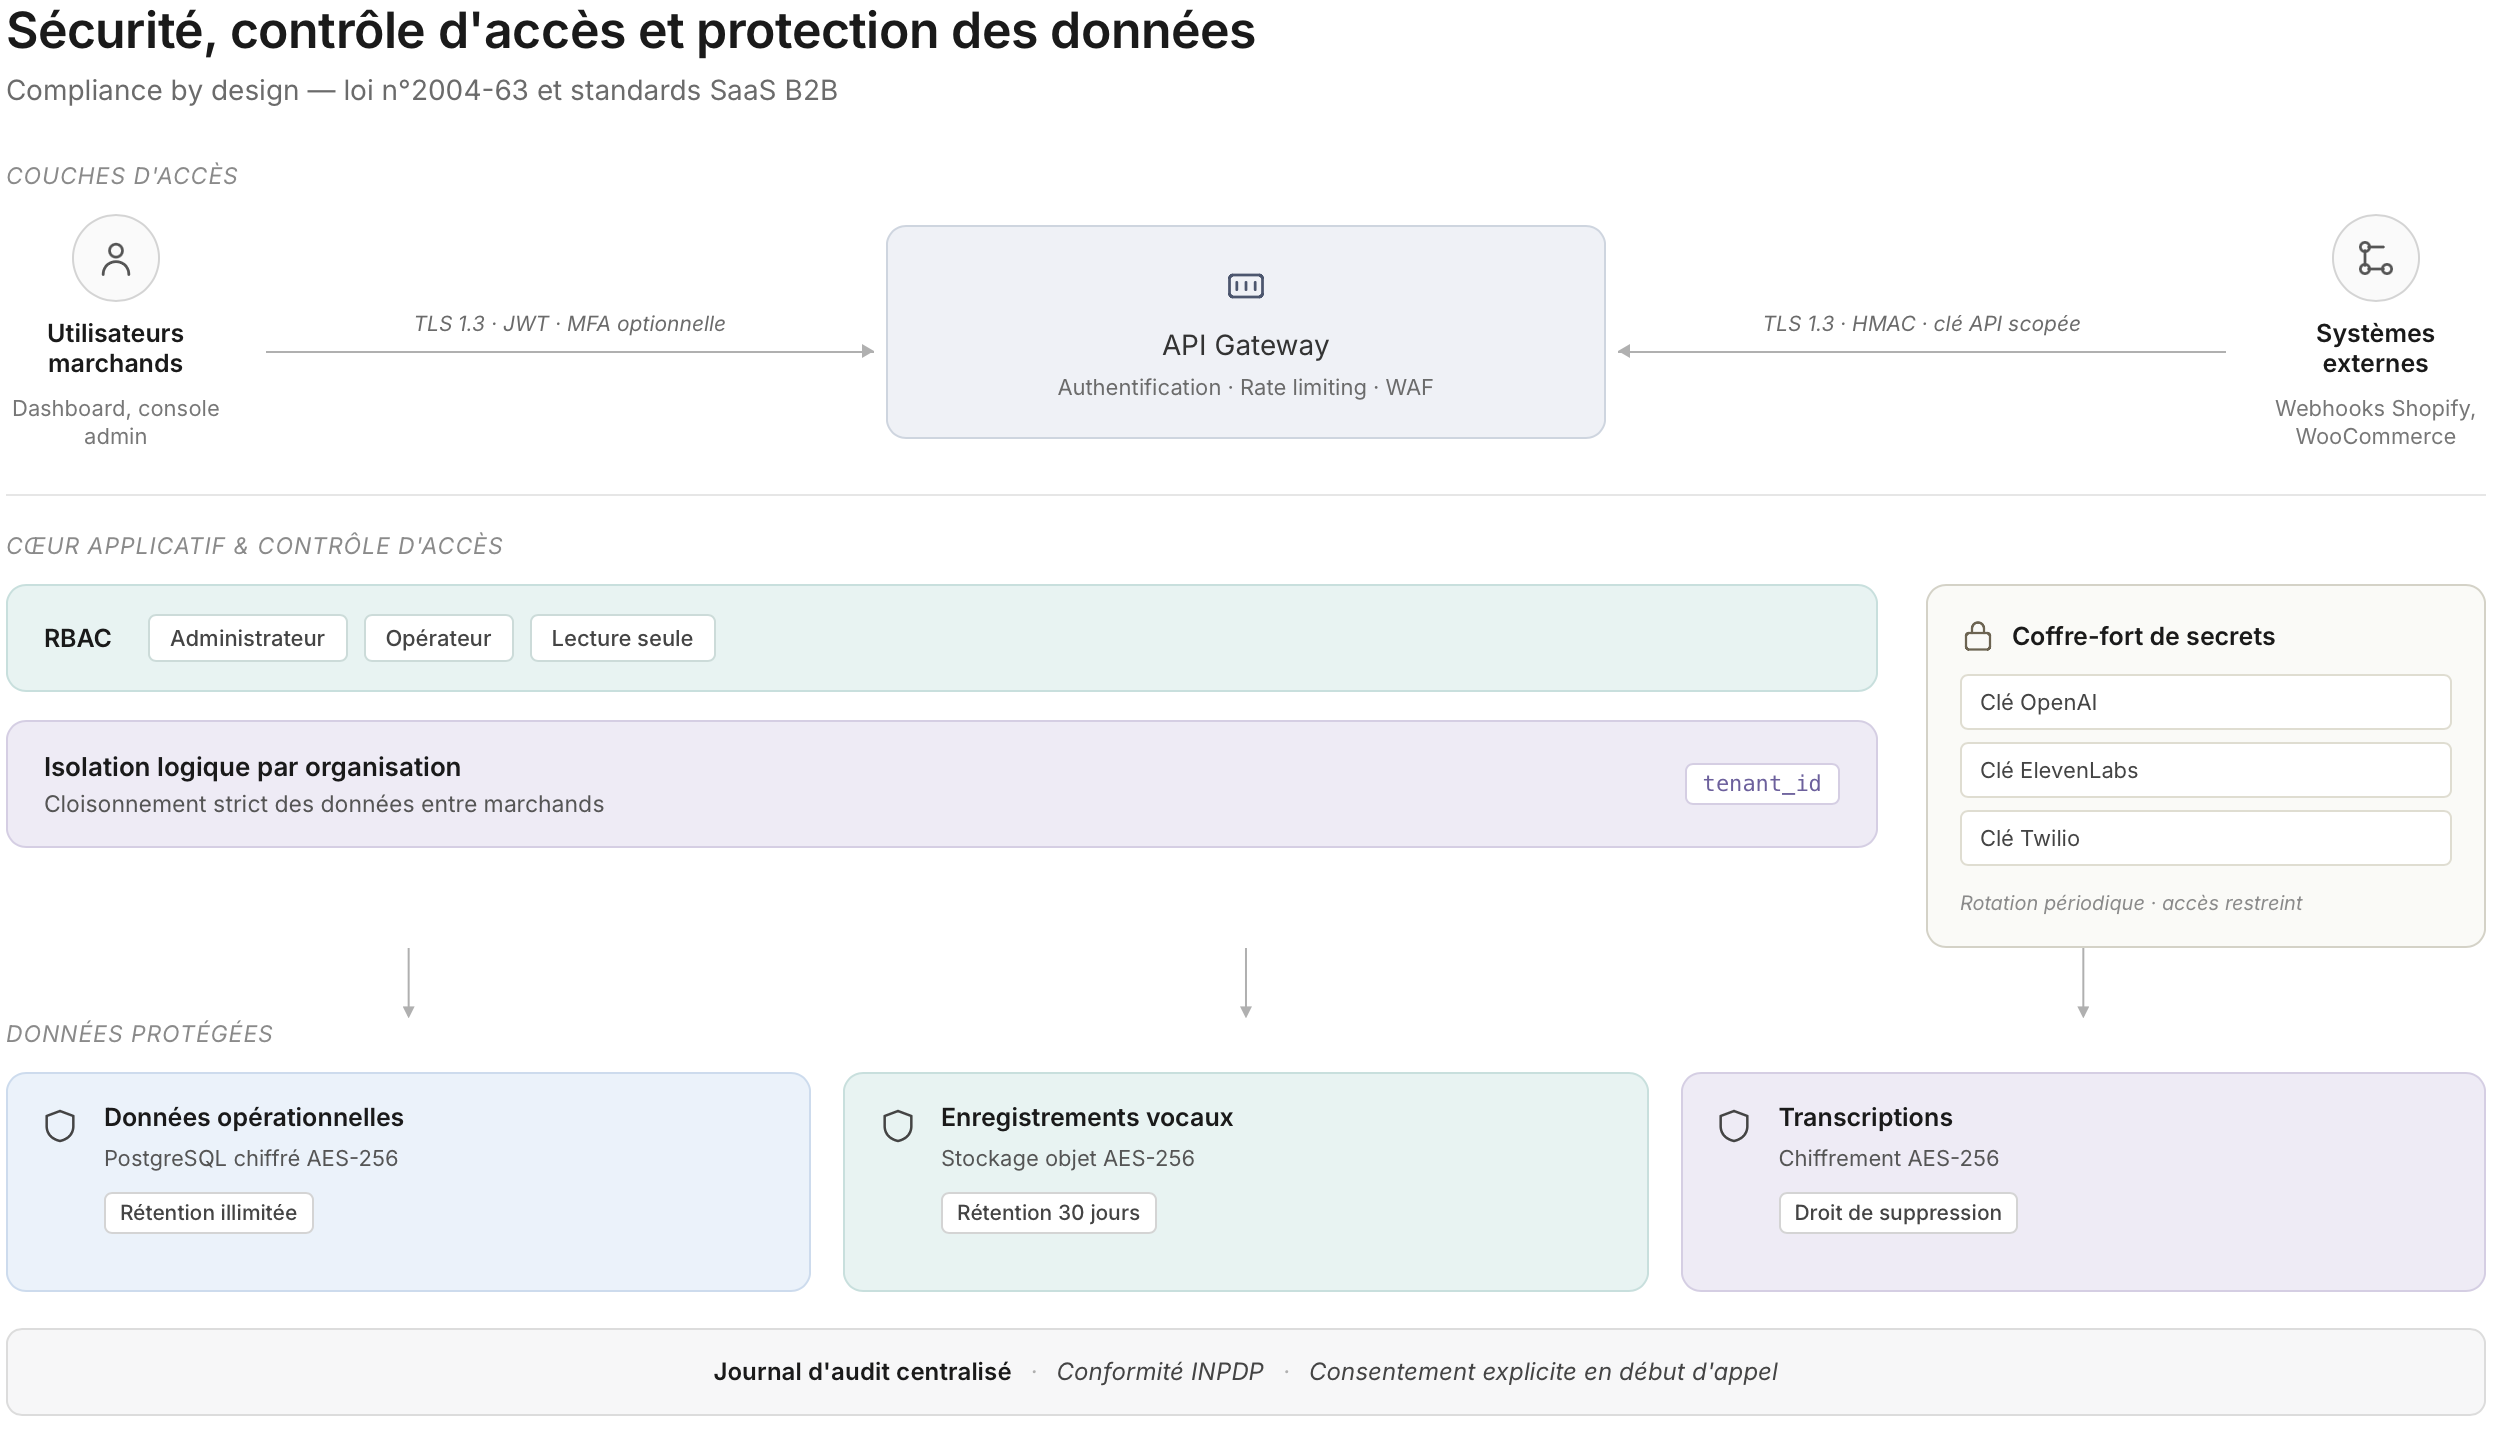
\includegraphics[width=\textwidth]{figures/securite_donnees_vocallia.png}
\caption{Architecture de sécurité et de protection des données — Vocallia}
\label{fig:securite_donnees}
\end{figure}

\subsection{Taxonomie des données manipulées}
\label{subsec:donnees_taxonomie}

Vocallia manipule cinq catégories de données, chacune soumise à des règles de traitement spécifiques. Les \textbf{données d'identité marchand} sont des données B2B classiques. Les \textbf{données opérationnelles} (commandes, statuts, métriques) appartiennent au patrimoine informationnel du marchand. Les \textbf{données personnelles des clients finaux} (numéros de téléphone, prénoms éventuels) sont les plus sensibles~: Vocallia y agit comme sous-traitant au sens de la loi n°2004-63, le marchand restant responsable du traitement. Les \textbf{enregistrements vocaux et transcriptions} constituent une catégorie particulière à laquelle la législation accorde une protection renforcée. Les \textbf{secrets techniques} (clés API, tokens, certificats) requièrent enfin une protection cryptographique systématique.

\subsection{Authentification, autorisation et isolation}
\label{subsec:donnees_authn_authz}

L'authentification des utilisateurs marchands repose sur un schéma email~/~mot de passe avec hachage robuste, complété d'une option de double authentification pour les comptes administrateur. Les sessions reposent sur des tokens JWT à durée de vie courte, accompagnés de tokens de rafraîchissement. L'authentification machine-to-machine (webhooks, API d'intégration) repose sur des clés API longues, scopées par organisation et par capacité, révocables individuellement. Au-dessus de l'authentification, un mécanisme de \textbf{contrôle d'accès basé sur les rôles} (RBAC) restreint chaque action aux rôles autorisés.

L'isolation logique entre clients constitue une exigence fondamentale d'un SaaS B2B~: aucun marchand ne doit jamais accéder aux données d'un autre. Vocallia implémente cette isolation par un pattern \emph{shared database, shared schema} avec rattachement systématique de chaque enregistrement à un identifiant d'organisation, et application de filtres au niveau de la couche d'accès aux données. Pour les comptes Pro relevant de secteurs sensibles, une option d'\textbf{isolation physique} (instance dédiée, base de données dédiée) est documentée et proposable sur devis.

\subsection{Gestion des secrets et protection des données vocales}
\label{subsec:donnees_secrets_vocal}

Les clés d'accès aux fournisseurs externes sont stockées dans un \textbf{coffre-fort de secrets} dédié (HashiCorp Vault, AWS Secrets Manager ou équivalent), jamais dans le code source ni dans des fichiers de configuration en clair. Aucune clé n'est exposée côté frontend~: tous les appels aux fournisseurs externes transitent par le backend, qui agit comme proxy sécurisé. Cette discipline élimine la classe de vulnérabilités la plus fréquente dans les architectures naïves.

Les enregistrements audio et transcriptions sont chiffrés au repos et en transit selon les standards éprouvés du secteur. Leur durée de rétention par défaut est de 30~jours, conforme à l'engagement réglementaire pris vis-à-vis de l'INPDP et explicitement annoncé aux clients finaux dans le message d'introduction d'appel. Cette rétention courte est aussi un choix d'architecture sécurité~: moins de données conservées signifie moins de surface d'attaque. Au-delà de la période de rétention, les données sont supprimées de manière irréversible. Une procédure d'effacement à la demande est prévue pour les clients finaux qui en feraient la requête via leur marchand.

\subsection{Conformité INPDP et logique réglementaire}
\label{subsec:donnees_inpdp}

La conformité à la loi n°2004-63 est intégrée par conception (\emph{compliance by design}) selon trois principes structurants. Le \textbf{consentement explicite} est obtenu en début d'appel par l'annonce de la nature automatisée et du droit du destinataire de demander un transfert humain — annonce non contournable et journalisée. La \textbf{minimisation des données} guide l'architecture~: aucune donnée sensible n'est collectée si elle n'est pas strictement nécessaire à la fonction. La \textbf{traçabilité des traitements} est assurée par un journal d'audit centralisé. Une démarche proactive d'engagement avec l'INPDP est prévue avant tout déploiement commercial à grande échelle.

\begin{quote}
\textbf{Sécurité comme avantage concurrentiel.} La rigueur sécurité et conformité décrite ici n'est pas un coût~: c'est un actif stratégique. Tout concurrent international souhaitant pénétrer le marché tunisien devra investir dans une conformité INPDP qu'il ne possède pas. Tout concurrent local moins rigoureux portera un risque juridique latent qui se matérialisera au premier contentieux. Vocallia, ayant intégré la conformité ab initio, transforme chaque renforcement réglementaire futur en avantage concurrentiel — exactement comme l'analyse PESTEL l'avait anticipé en section~2.1.
\end{quote}

%%%%%%%%%%%%%%%%%%%%%%%%%%%%%%%%%%%%%%%%%%%%%%%%%%%%%%%%%%%%%%%%%%%%%%%%%%%
\section{Scalabilité, résilience et observabilité}
\label{sec:scalabilite}
%%%%%%%%%%%%%%%%%%%%%%%%%%%%%%%%%%%%%%%%%%%%%%%%%%%%%%%%%%%%%%%%%%%%%%%%%%%

Une architecture peut être fonctionnellement correcte et néanmoins défaillir sous charge, lors de pannes externes, ou par incapacité à diagnostiquer ses propres dysfonctionnements. Trois propriétés transverses gouvernent la robustesse opérationnelle de Vocallia~: la scalabilité, la résilience et l'observabilité.

\subsection{Scalabilité de l'architecture}
\label{subsec:scal_architecture}

L'architecture de Vocallia est conçue pour scaler horizontalement, en ajoutant des instances de services plutôt qu'en augmentant la puissance d'une instance unique. Cinq choix structurels rendent ce scaling possible~: des \textbf{services applicatifs stateless}, dans lesquels aucune information de session n'est conservée localement~; une \textbf{file de messages} qui découple producteurs et consommateurs et absorbe les pics de charge~; un \textbf{cache distribué} qui réduit la pression sur la base de données~; une \textbf{séparation lecture/écriture} permettant de scaler les requêtes analytiques sans affecter les performances transactionnelles~; et un mécanisme d'\textbf{auto-scaling} qui ajuste le nombre d'instances en fonction de la charge mesurée. L'ensemble permet une montée en charge progressive cohérente avec la trajectoire commerciale projetée, sans refonte architecturale entre les paliers.

\subsection{Résilience et gestion des erreurs}
\label{subsec:scal_resilience}

La résilience de Vocallia repose sur le principe que toute dépendance externe peut défaillir, et qu'une défaillance ne doit jamais se propager en panne globale. Quatre mécanismes structurent cette résilience. Les \textbf{retries avec backoff exponentiel} sont implémentés sur tous les appels aux API externes, évitant l'effet d'avalanche en cas de saturation côté fournisseur. Les \textbf{circuit breakers} interrompent automatiquement les requêtes vers une dépendance en panne avérée, restaurant le trafic après une période de test. La \textbf{dead-letter queue} capture les jobs qui ont définitivement échoué après tous les retries, permettant leur analyse manuelle plutôt que leur perte silencieuse. Enfin, la \textbf{stratégie multi-fournisseurs} sur les couches IA et téléphonie ouvre la possibilité de basculer vers un fournisseur de secours en cas d'incident prolongé chez le fournisseur principal — exigence stratégique formalisée dans l'analyse SWOT.

\subsection{Observabilité opérationnelle}
\label{subsec:scal_observabilite}

L'observabilité repose sur les trois piliers classiques (Sridharan, 2018)~: les \textbf{logs}, les \textbf{métriques} et les \textbf{traces distribuées}. Vocallia instrumente l'ensemble de ses services pour produire ces trois types de signaux, agrégés dans une plateforme unifiée. Le tableau~\ref{tab:kpi_techniques} synthétise les principaux indicateurs surveillés en production et les actions associées en cas de dépassement.

\begin{table}[H]
\centering
\caption{Indicateurs techniques surveillés en production}
\label{tab:kpi_techniques}
\begin{tabular}{|p{5cm}|p{4cm}|p{5cm}|}
\hline
\textbf{Indicateur} & \textbf{Cible opérationnelle} & \textbf{Action en cas de dépassement} \\
\hline
Latence p95 par tour de parole & Proche de la cible & Alerte équipe technique, investigation \\
\hline
Taux d'erreur des appels API IA & Faible (<1~\%) & Bascule vers fournisseur secondaire \\
\hline
Taux d'échec de webhook entrant & Très faible & Investigation côté marchand ou Vocallia \\
\hline
Disponibilité globale du service & Élevée et continue & Post-mortem si non atteinte sur le mois \\
\hline
Taux de fallback humain involontaire & Maîtrisé & Analyse des causes, ajustement scripts \\
\hline
Score moyen de confiance STT & Élevé en moyenne & Ajustement du lexique et du \emph{prompt biasing} \\
\hline
\end{tabular}
\end{table}

Au-delà des indicateurs, des \textbf{alertes proactives} notifient l'équipe d'astreinte en cas de défaillance critique avant que les marchands n'en soient impactés. Cette posture proactive est essentielle dans un contexte SaaS B2B où chaque interruption non détectée se traduit en perte de confiance.

\begin{quote}
\textbf{Résilience face aux défaillances de fournisseurs externes.} Le scénario opérationnel le plus redouté n'est pas la défaillance interne, qu'une équipe maîtrisée peut diagnostiquer et corriger~; c'est la défaillance d'un fournisseur tiers sur lequel Vocallia n'a aucun levier direct. La réponse architecturale est triple~: substituabilité par design, dégradation gracieuse (le système continue de fonctionner avec une qualité réduite plutôt que de s'arrêter) et communication transparente vers les marchands. Cette discipline transforme un risque potentiel en simple incident géré.
\end{quote}

%%%%%%%%%%%%%%%%%%%%%%%%%%%%%%%%%%%%%%%%%%%%%%%%%%%%%%%%%%%%%%%%%%%%%%%%%%%
\section{Déploiement et exploitabilité}
\label{sec:deploiement}
%%%%%%%%%%%%%%%%%%%%%%%%%%%%%%%%%%%%%%%%%%%%%%%%%%%%%%%%%%%%%%%%%%%%%%%%%%%

Une architecture exploitable n'est pas seulement une architecture qui fonctionne~: c'est une architecture que l'on peut déployer rapidement, mettre à jour sans risque, faire évoluer sans dette accumulée et opérer avec une équipe restreinte. Ces propriétés sont particulièrement critiques pour Vocallia, dont l'équipe initiale est volontairement réduite (cf. section~3.6). La figure~\ref{fig:deploiement_monitoring} synthétise l'articulation entre pipeline de livraison, infrastructure cloud et dispositifs de résilience et d'observabilité.

\begin{figure}[H]
\centering
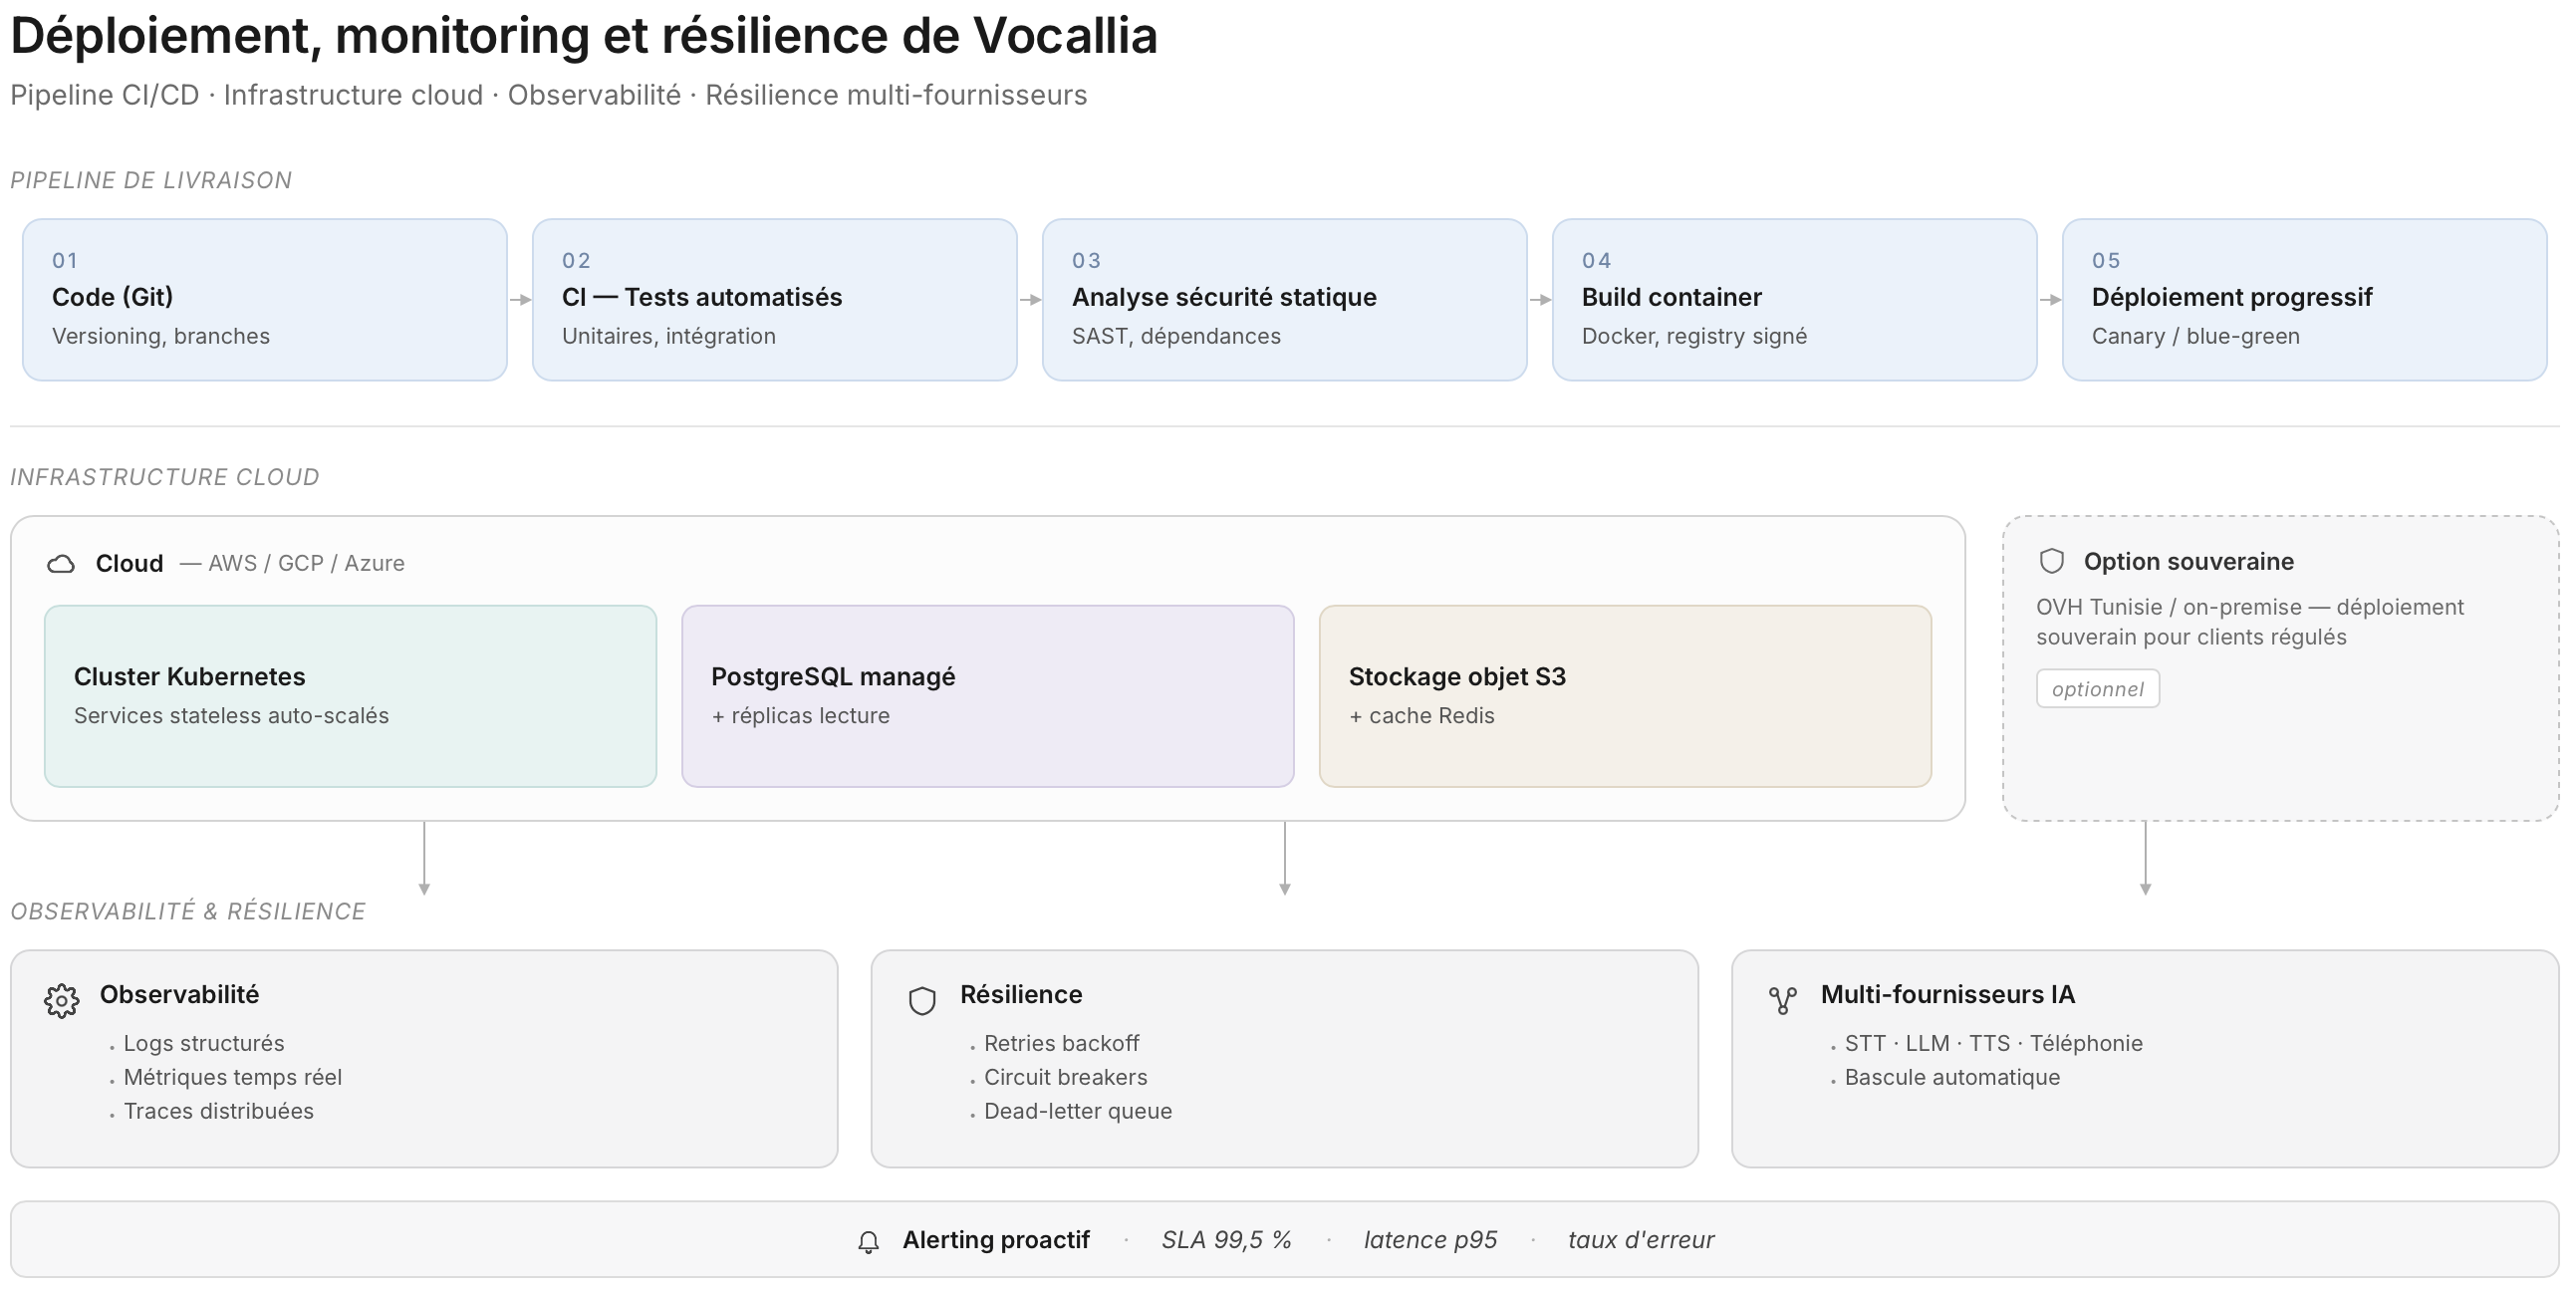
\includegraphics[width=\textwidth]{figures/deploiement_monitoring_vocallia.png}
\caption{Déploiement, monitoring et résilience de Vocallia}
\label{fig:deploiement_monitoring}
\end{figure}

\subsection{Approche cloud et infrastructure}
\label{subsec:deploiement_cloud}

Vocallia adopte une approche \emph{cloud-first} fondée sur des services managés. Le déploiement initial cible un fournisseur cloud unique (AWS, GCP ou Azure, selon les arbitrages tarifaires et de proximité régionale) avec une architecture neutre vis-à-vis du fournisseur~: l'usage de standards ouverts (Docker, Kubernetes, PostgreSQL, Redis) garantit qu'une migration future reste réalisable sans réécriture profonde. Pour les comptes institutionnels relevant de secteurs sensibles, une option de \textbf{déploiement souverain} sur infrastructure tunisienne (OVH Tunisie ou hébergement privé) est documentée. Cette option répond à la fois à des exigences éventuelles de souveraineté des données et aux préoccupations environnementales évoquées en section~2.1.

\subsection{Conditions de mise en production}
\label{subsec:deploiement_prod}

Le passage du MVP à la production opérationnelle est conditionné à une liste de critères techniques explicites~: couverture de tests automatisés sur les chemins critiques, monitoring complet déployé avec alertes configurées, procédures de \emph{runbook} documentées pour les incidents les plus probables, sauvegardes automatisées avec test de restauration validé, plan de continuité d'activité rédigé, audit de sécurité initial réalisé et procédure d'engagement INPDP initiée. Ces critères constituent une \textbf{checklist de production-readiness} dont le franchissement est une décision discrète, et non un glissement progressif.

\subsection{Maintenabilité et évolutivité}
\label{subsec:deploiement_maintenance}

Trois pratiques structurent la maintenabilité du système. L'\textbf{infrastructure as code} versionne l'ensemble de la configuration cloud, rendant les déploiements reproductibles et les modifications auditables. La \textbf{containerisation systématique} standardise les environnements de développement, de test et de production. Le \textbf{pipeline CI/CD} automatise tests, analyses statiques de qualité et de sécurité, et déploiements selon une stratégie progressive (\emph{canary} ou \emph{blue/green}) qui permet de détecter les régressions avant qu'elles n'affectent l'ensemble des marchands. L'évolutivité fonctionnelle est assurée par la modularité décrite en section~\ref{sec:architecture_logique}~: l'ajout d'un nouveau cas d'usage consiste essentiellement en l'ajout d'un scénario conversationnel et d'un connecteur d'intégration, sans toucher aux modules transverses.

\subsection{Trajectoire MVP-vers-production}
\label{subsec:deploiement_mvp}

La trajectoire technique de Vocallia s'articule en trois phases. La \textbf{phase MVP} (mois~1 à~3) délivre un système monolithique léger couvrant le scénario unique de confirmation de commande, intégré à une seule plateforme et déployé sur une infrastructure cloud minimale. La \textbf{phase pilote} (mois~3 à~6) introduit la modularisation progressive (extraction des services critiques), enrichit les intégrations, déploie le monitoring complet et engage la procédure INPDP. La \textbf{phase production} (à partir du mois~6) bascule sur l'architecture cible décrite dans le présent chapitre, avec multi-fournisseurs actifs, isolation multi-tenant durcie et observabilité complète. Cette trajectoire garantit que chaque investissement technique est calé sur un palier d'usage qui le justifie économiquement — discipline d'architecture frugale cohérente avec les contraintes de financement définies au chapitre précédent.

%%%%%%%%%%%%%%%%%%%%%%%%%%%%%%%%%%%%%%%%%%%%%%%%%%%%%%%%%%%%%%%%%%%%%%%%%%%
\section{Limites techniques et mesures de mitigation}
\label{sec:limites_mitigation}
%%%%%%%%%%%%%%%%%%%%%%%%%%%%%%%%%%%%%%%%%%%%%%%%%%%%%%%%%%%%%%%%%%%%%%%%%%%

Aucune architecture n'est sans limite. La rigueur d'un projet technique se mesure à sa capacité à identifier explicitement ses points de fragilité et à associer à chacun une mesure de mitigation crédible. Le tableau~\ref{tab:limites_mitigation} synthétise les cinq limites principales de Vocallia et la stratégie de mitigation associée.

\begin{table}[H]
\centering
\caption{Limites techniques de Vocallia et mesures de mitigation}
\label{tab:limites_mitigation}
\begin{tabular}{|p{3.5cm}|p{4.5cm}|p{6cm}|}
\hline
\textbf{Limite} & \textbf{Nature du risque} & \textbf{Mesures de mitigation} \\
\hline
Variabilité dialectale & Variations régionales et générationnelles du darija mal couvertes par les modèles génériques & \emph{Prompt biasing} avec lexique tunisien~; constitution d'un corpus propriétaire à partir des appels traités~; cycle d'amélioration mensuel des scripts~; fallback humain en cas de confiance faible \\
\hline
Latence cumulée & Le pipeline STT~$\to$~LLM~$\to$~TTS peut dépasser ponctuellement la cible de latence & Streaming bout en bout~; mise en cache des introductions vocales~; \emph{filler conversationnels} masquant la latence~; surveillance p95 et alerting \\
\hline
Dépendance fournisseurs tiers & Hausse tarifaire, interruption de service ou changement de CGU des API externes & Architecture multi-fournisseurs avec adaptateurs interchangeables~; circuit breakers~; possibilité de bascule vers fournisseur secondaire \\
\hline
Fiabilité de la téléphonie sortante & Échec de connexion, qualité audio dégradée, blocage par opérateurs anti-spam & Stratégie de retry sur appels échoués~; surveillance des taux par opérateur destinataire~; partenariat futur potentiel avec opérateur local \\
\hline
Volatilité des prix d'API IA & Modification des tarifs OpenAI / ElevenLabs impactant la marge brute & Veille tarifaire continue~; possibilité de bascule vers alternatives (Claude, Mistral, Coqui)~; économies d'échelle avec la croissance du volume \\
\hline
\end{tabular}
\end{table}

Au-delà du tableau, deux principes transverses gouvernent la posture de Vocallia face à ces limites. Le premier est la \textbf{transparence assumée}~: aucune limite n'est dissimulée aux marchands. Lorsqu'une interaction sort du périmètre de fiabilité de l'IA, le marchand est notifié et le rappel humain est explicitement recommandé. Cette transparence préserve efficacement la confiance, bien plus qu'une promesse universelle qui se révélerait fausse. Le second est la \textbf{conversion progressive des limites en avantages compétitifs}~: chaque appel traité enrichit le corpus dialectal propriétaire de Vocallia. Ce qui constitue aujourd'hui une limite — couverture imparfaite des sous-registres dialectaux — devient demain un actif que les concurrents entrants ne pourront pas répliquer instantanément, exactement le mécanisme de \emph{flywheel} décrit en figure~2.9 du chapitre~2.

\begin{quote}
\textbf{Discipline face aux limites.} La force d'une architecture ne réside pas dans l'absence de limites — qui serait illusoire — mais dans le fait que chaque limite est identifiée explicitement, surveillée techniquement, mitigée concrètement et inscrite dans une dynamique d'amélioration mesurable. Aucune des cinq limites ci-dessus n'est rédhibitoire pour le lancement~; toutes sont instrumentées et adressées par une mesure de mitigation directement opérationnelle.
\end{quote}

%%%%%%%%%%%%%%%%%%%%%%%%%%%%%%%%%%%%%%%%%%%%%%%%%%%%%%%%%%%%%%%%%%%%%%%%%%%
\section{Conclusion}
\label{sec:conclusion_chap4}
%%%%%%%%%%%%%%%%%%%%%%%%%%%%%%%%%%%%%%%%%%%%%%%%%%%%%%%%%%%%%%%%%%%%%%%%%%%

L'analyse technique conduite dans ce chapitre établit quatre conclusions qui valident la viabilité technique de Vocallia.

\textbf{La solution est techniquement réalisable avec les technologies actuelles.} Chacun des composants du pipeline conversationnel — reconnaissance vocale, modèle de langage, synthèse vocale, téléphonie programmable — est aujourd'hui disponible en mode service à des conditions économiques compatibles avec le pricing défini en section~3.8. Le coût variable par appel de deux minutes, estimé autour de 0{,}27~DT, est cohérent avec un prix d'entrée Starter de 0{,}79~DT par appel et préserve une marge brute soutenable de l'ordre de 65~\%. La latence cible reste atteignable grâce au streaming et à une orchestration soignée, et la couverture dialectale est suffisante au lancement avec les mécanismes de mitigation mis en place.

\textbf{L'architecture est cohérente avec les objectifs produit.} La modularité en sept blocs métier traduit directement la roadmap d'extension multi-cas d'usage. La séparation en cinq couches techniques garantit l'évolutivité, la testabilité et la substituabilité des fournisseurs. La conception multi-tenant et la conformité INPDP intégrée ab initio sont les conditions techniques de la promesse commerciale formulée aux marchands. Aucune décision technique n'est gratuite~: chacune découle d'une exigence produit ou d'une contrainte explicitement identifiée.

\textbf{Les risques techniques sont identifiés, surveillés et adressés.} Les cinq limites principales — variabilité dialectale, latence, dépendance fournisseurs, fiabilité téléphonique, volatilité tarifaire — sont chacune associées à une mesure de mitigation opérationnelle. La résilience est assurée par la redondance multi-fournisseurs, les retries, les circuit breakers et la dégradation gracieuse. L'observabilité complète permet le diagnostic rapide et l'amélioration continue. Aucun risque technique identifié ne constitue un obstacle rédhibitoire au lancement.

\textbf{L'architecture est évolutive, pas figée.} La trajectoire MVP~$\to$~pilote~$\to$~production permet de calibrer chaque investissement technique sur le palier d'usage qui le justifie. La modularité interne autorise l'ajout de nouveaux cas d'usage sans refonte. L'option de déploiement souverain ouvre l'accès aux secteurs institutionnels sensibles. Le système est conçu pour grandir avec Vocallia, pas pour être réécrit à chaque palier.

L'ensemble de ces éléments converge vers une conclusion sans ambiguïté~: \emph{Vocallia est techniquement viable}. L'architecture proposée n'est ni surdimensionnée pour le lancement ni sous-dimensionnée pour la croissance~; elle est calibrée sur la trajectoire commerciale projetée au chapitre précédent, et conçue pour servir la promesse produit définie au chapitre~3, dans les contraintes de marché établies au chapitre~2.

Le chapitre suivant prolonge cette analyse sur le terrain de la viabilité financière et de l'exécution opérationnelle~: budget initial, plan de financement, chronogramme de lancement, jalons critiques, et conditions de transformation de la solution technique en activité économique pérenne.
%%%%%%%%%%%%%%%%%%%%%%%%%%%%%%%%%%%%%%%%%%%%%%%%%%%%%%%%%%%%%%%%%%%%%%%%%%%
\chapter{Étude de la viabilité financière et plan d'exécution}
\label{Chapitre_5}
%%%%%%%%%%%%%%%%%%%%%%%%%%%%%%%%%%%%%%%%%%%%%%%%%%%%%%%%%%%%%%%%%%%%%%%%%%%
\section{Introduction}
\label{sec:intro_chap5}
%%%%%%%%%%%%%%%%%%%%%%%%%%%%%%%%%%%%%%%%%%%%%%%%%%%%%%%%%%%%%%%%%%%%%%%%%%%

Les chapitres précédents ont successivement démontré que Vocallia répondait à un besoin de marché identifié et quantifié (chapitre~2), qu'il pouvait être structuré en un modèle commercial scalable et défendable (chapitre~3), et qu'il reposait sur une architecture technique réalisable, résiliente et conforme aux contraintes réglementaires locales (chapitre~4). Reste un dernier test, le plus exigeant aux yeux d'un jury comme d'un investisseur~: la viabilité financière. Une opportunité de marché, aussi réelle soit-elle, ne se transforme en entreprise pérenne que si la trajectoire économique projetée est cohérente, les hypothèses calibrées avec prudence, et les jalons d'exécution alignés sur la capacité d'investissement disponible.

L'objet de ce chapitre n'est pas de chiffrer des coûts ou des revenus pour eux-mêmes, mais d'évaluer dans quelles conditions Vocallia peut franchir, sans rupture financière, la séquence MVP~$\to$~pilote~$\to$~production identifiée au chapitre~4, tout en restant fidèle aux fondations du modèle économique posées au chapitre~3. L'analyse procède en trois temps. Elle pose d'abord les hypothèses financières structurantes, l'investissement initial nécessaire et la structure de coûts d'exploitation. Elle construit ensuite des projections de revenus, un compte de résultat prévisionnel et un seuil de rentabilité, déclinés selon trois scénarios — prudent, central et ambitieux — afin de tester la robustesse du modèle. Elle examine enfin le plan de financement, les indicateurs de rentabilité, le plan d'exécution opérationnelle, l'impact attendu et la cartographie des risques.

Toutes les valeurs chiffrées de ce chapitre sont présentées comme des \emph{estimations indicatives}, à valider à mesure de l'avancement du projet. Elles s'appuient sur les coûts unitaires établis au chapitre~4 — coût variable d'environ 0{,}27~DT par appel de deux minutes, soutenant une marge brute de l'ordre de 65~\% sur le palier Starter — et sur des hypothèses prudentes pour une clientèle PME tunisienne en phase d'amorçage. Lorsque les données disponibles ne permettent pas un calcul rigoureux, les éléments sont présentés comme des hypothèses à valider, et non comme des certitudes. Cette discipline est, in fine, la meilleure défense du chapitre~: un plan financier crédible n'est pas un plan optimiste, c'est un plan dont chaque chiffre peut être discuté, contesté et défendu.

%%%%%%%%%%%%%%%%%%%%%%%%%%%%%%%%%%%%%%%%%%%%%%%%%%%%%%%%%%%%%%%%%%%%%%%%%%%
\section{Hypothèses financières et cadre de projection}
\label{sec:hypotheses_financieres}
%%%%%%%%%%%%%%%%%%%%%%%%%%%%%%%%%%%%%%%%%%%%%%%%%%%%%%%%%%%%%%%%%%%%%%%%%%%

\subsection{Logique de lancement et horizon de projection}
\label{subsec:logique_lancement}

L'horizon retenu pour la projection financière est de \textbf{36~mois} à compter du lancement opérationnel, en cohérence avec la trajectoire commerciale modélisée au chapitre~3 et avec la trajectoire technique du chapitre~4 (MVP~$\to$~pilote~$\to$~production). Trois raisons justifient cet horizon. D'abord, il correspond à la durée typique d'un cycle d'amorçage SaaS B2B, suffisamment long pour observer une trajectoire de revenus récurrents mais suffisamment court pour rester crédible sans extrapolation hasardeuse. Ensuite, il coïncide avec la fenêtre concurrentielle de 18 à 36~mois identifiée au chapitre~2~: c'est dans cet intervalle que Vocallia doit chercher à convertir son avance temporelle en actifs durables. Enfin, il permet de séquencer les jalons financiers de manière lisible — couverture progressive des charges fixes, équilibre opérationnel, et, à terme, génération éventuelle de cash réinvestissable.

\subsection{Hypothèses financières clés}
\label{subsec:hypotheses_cles}

L'ensemble des projections du chapitre repose sur un socle d'hypothèses explicitement formulées et reliées aux chapitres antérieurs. Le tableau~\ref{tab:hypotheses_financieres} les synthétise.

\begin{table}[H]
\centering
\caption{Hypothèses financières clés — Vocallia (horizon 36 mois)}
\label{tab:hypotheses_financieres}
\begin{tabular}{|p{4.5cm}|p{5cm}|p{5cm}|}
\hline
\textbf{Catégorie} & \textbf{Hypothèse retenue} & \textbf{Source / justification} \\
\hline
Plan d'entrée Starter & 79~DT/mois pour 100 appels inclus & Chapitre~3, section~3.8 \\
\hline
Prix unitaire effectif Starter & $\sim$0{,}79~DT par appel & Forfait~/~appels inclus \\
\hline
Coût variable moyen par appel (2~min) & $\sim$0{,}27~DT & Chapitre~4, structure de coûts API \\
\hline
Marge brute du plan Starter & $\sim$65~\% & Calcul direct $(0{,}79 - 0{,}27)/0{,}79$ \\
\hline
ARPU pondéré (mix des 3 paliers) & $\sim$120~DT/mois & Chapitre~3, section~3.9 \\
\hline
Contribution moyenne par client actif & $\sim$78~DT/mois & ARPU~$\times$~marge brute \\
\hline
Churn mensuel cible & 5 à 8~\% & Hypothèse prudente pour clientèle PME en amorçage \\
\hline
LTV/CAC visé & supérieur à 3~:~1 & Seuil minimal généralement attendu en SaaS B2B \\
\hline
CAC payback visé & inférieur à 6 mois & Discipline d'exécution PLG \\
\hline
Charges fixes mensuelles (an~1) & $\sim$1\,200~DT & Équipe restreinte, infra mutualisée \\
\hline
Charges fixes mensuelles (an~3) & $\sim$3\,500~DT & Montée progressive de l'équipe \\
\hline
Régime fiscal & Startup Act (exonération initiale) & Loi n°2018-20 \\
\hline
\end{tabular}
\end{table}

\paragraph{Synthèse analytique.} Ces hypothèses ne sont ni audacieuses ni promotionnelles~: elles reprennent les valeurs déjà défendues dans les chapitres précédents et les inscrivent dans un cadre quantitatif unifié. Toute lecture critique du présent chapitre peut donc remonter, hypothèse par hypothèse, vers la justification d'origine — condition académique d'une projection financière sérieuse. Les valeurs proposées doivent être lues comme des ordres de grandeur prudents, à recalibrer dès que les premières données opérationnelles seront disponibles.

\subsection{Logique de scénarios}
\label{subsec:logique_scenarios}

À l'image du chapitre~3, trois scénarios encadrent la projection. Le \textbf{scénario prudent} suppose un rythme d'acquisition lent (1 à 2 nouveaux clients payants par mois), un churn proche de la borne haute et une montée en charge limitée sur les paliers supérieurs. Le \textbf{scénario central} reflète la trajectoire considérée comme la plus probable~: 3 à 4 acquisitions mensuelles, churn autour de 6~\%, mix progressif Starter~$\to$~Croissance. Le \textbf{scénario ambitieux} traduit l'effet d'une diffusion accélérée par le bouche-à-oreille des e-commerçants tunisiens et l'activation rapide des partenariats de distribution. Aucun de ces scénarios ne suppose une rupture technologique externe ni un investissement publicitaire massif~: ils restent dans le périmètre des moyens internes raisonnablement mobilisables par une startup en phase d'amorçage.

%%%%%%%%%%%%%%%%%%%%%%%%%%%%%%%%%%%%%%%%%%%%%%%%%%%%%%%%%%%%%%%%%%%%%%%%%%%
\section{Investissement initial}
\label{sec:investissement_initial}
%%%%%%%%%%%%%%%%%%%%%%%%%%%%%%%%%%%%%%%%%%%%%%%%%%%%%%%%%%%%%%%%%%%%%%%%%%%

L'investissement initial vise à amener Vocallia de l'état de projet à l'état de produit pilote opérationnel auprès des premiers clients payants. Il est dimensionné selon une logique \emph{minimum viable financing}~: couvrir strictement les besoins critiques pour franchir le premier palier de validation commerciale (5 à 10 clients pilotes actifs), et différer toute dépense non indispensable à un stade ultérieur où elle pourra, le cas échéant, être financée par les revenus générés. La figure~\ref{fig:budget_initial} en présente la décomposition.

\begin{figure}[H]
\centering
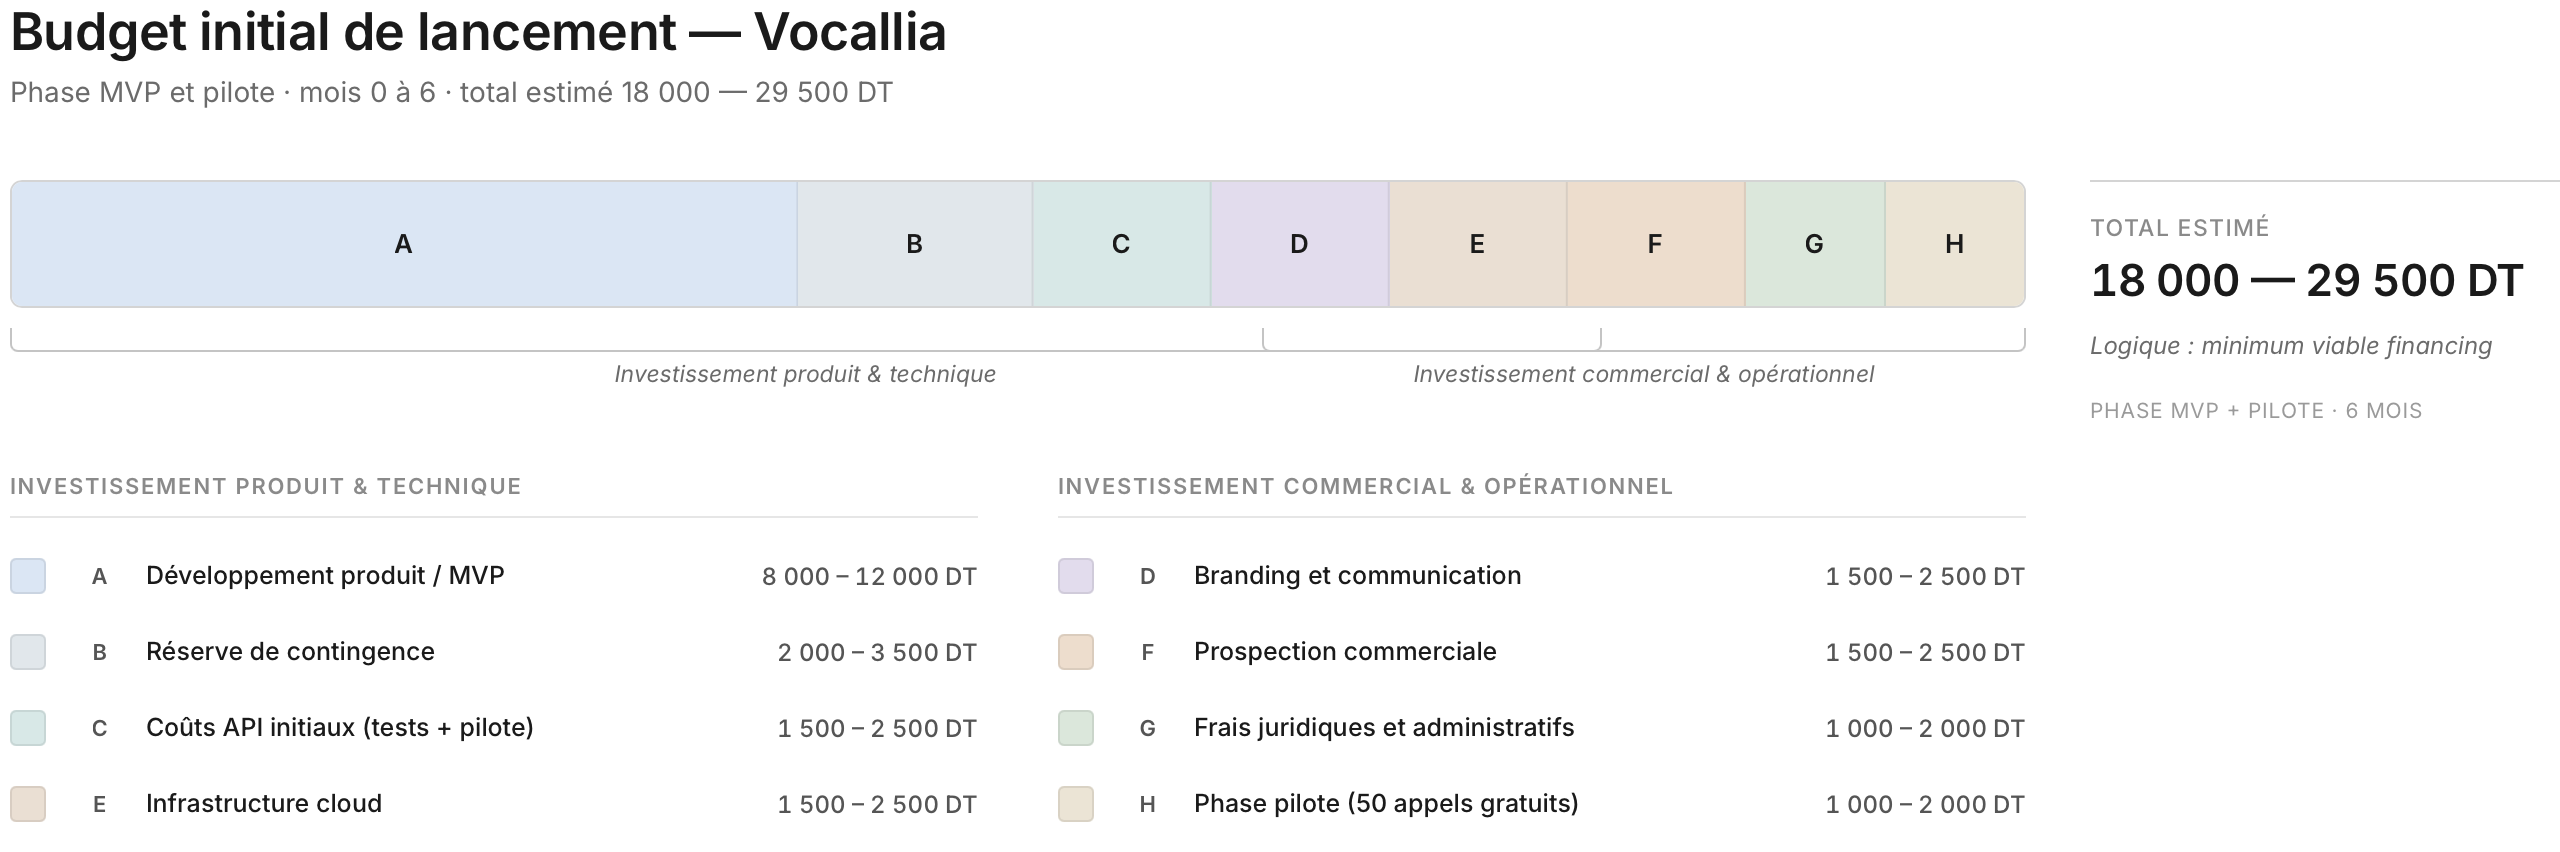
\includegraphics[width=\textwidth]{figures/budget-initial-lancement-vocallia.png}
\caption{Budget initial de lancement — phase MVP et pilote (mois 0--6)}
\label{fig:budget_initial}
\end{figure}

\begin{table}[H]
\centering
\caption{Investissement initial estimé — phase MVP et pilote (mois 0 à 6)}
\label{tab:investissement_initial}
\begin{tabular}{|p{5cm}|p{3cm}|p{6cm}|}
\hline
\textbf{Poste} & \textbf{Budget (DT)} & \textbf{Nature et justification} \\
\hline
Développement produit / MVP & 8\,000 — 12\,000 & Construction du pipeline conversationnel, dashboard, intégrations Shopify / WooCommerce \\
\hline
Infrastructure cloud et configuration technique & 1\,500 — 2\,500 & Mise en place initiale (Docker, Kubernetes managé, base de données, monitoring) \\
\hline
Coûts API initiaux (tests, calibrage, pilote) & 1\,500 — 2\,500 & STT, LLM, TTS et téléphonie sur volume de tests et premiers appels pilotes \\
\hline
Frais juridiques et administratifs & 1\,000 — 2\,000 & Constitution juridique, labellisation Startup Act, démarche INPDP préliminaire \\
\hline
Branding et communication & 1\,500 — 2\,500 & Identité visuelle, site web, landing page, vidéos de démonstration \\
\hline
Prospection commerciale initiale & 1\,500 — 2\,500 & Campagnes Meta Ads, outils CRM, déplacements, démonstrations directes \\
\hline
Phase pilote (50 appels gratuits par marchand) & 1\,000 — 2\,000 & Coût opérationnel des pilotes offerts (Product-Led Growth) \\
\hline
Réserve de contingence (10—15~\%) & 2\,000 — 3\,500 & Couverture des aléas techniques, juridiques et commerciaux \\
\hline
\textbf{Total estimé} & \textbf{18\,000 — 29\,500} & Budget de lancement minimum viable \\
\hline
\end{tabular}
\end{table}

\paragraph{Lecture stratégique.} Trois caractéristiques rendent cet investissement défendable. D'abord, une part significative du coût (développement produit) peut être valorisée comme contribution en nature des fondateurs, ce qui réduit le besoin de cash externe immédiat. Ensuite, le budget de prospection est calibré sur des canaux à coût marginal observé en phase exploratoire — la phase Muvaka d'avril 2025 ayant produit un coût par lead (CPL) de l'ordre de 0{,}36~euro, indicateur de \emph{génération de leads} et non de coût d'acquisition client confirmé, qui devra être validé une fois le premier cycle de conversion mesuré. Enfin, la réserve de contingence de l'ordre de 10 à 15~\% protège contre les aléas sans gonfler artificiellement le besoin de financement initial.

%%%%%%%%%%%%%%%%%%%%%%%%%%%%%%%%%%%%%%%%%%%%%%%%%%%%%%%%%%%%%%%%%%%%%%%%%%%
\section{Charges d'exploitation et structure de coûts}
\label{sec:charges_exploitation}
%%%%%%%%%%%%%%%%%%%%%%%%%%%%%%%%%%%%%%%%%%%%%%%%%%%%%%%%%%%%%%%%%%%%%%%%%%%

La structure de coûts de Vocallia présente une caractéristique stratégique majeure~: elle est \textbf{dominée par les coûts variables}, indexés sur le volume d'appels traités. Cette propriété, déjà soulignée au chapitre~3, est la condition mathématique de la scalabilité du modèle~: chaque client supplémentaire peut être servi sans déclencher de saut significatif de coûts fixes, sous réserve que la hausse soit absorbée par les capacités existantes de l'équipe. La figure~\ref{fig:structure_charges} en visualise la répartition.

\begin{figure}[H]
\centering
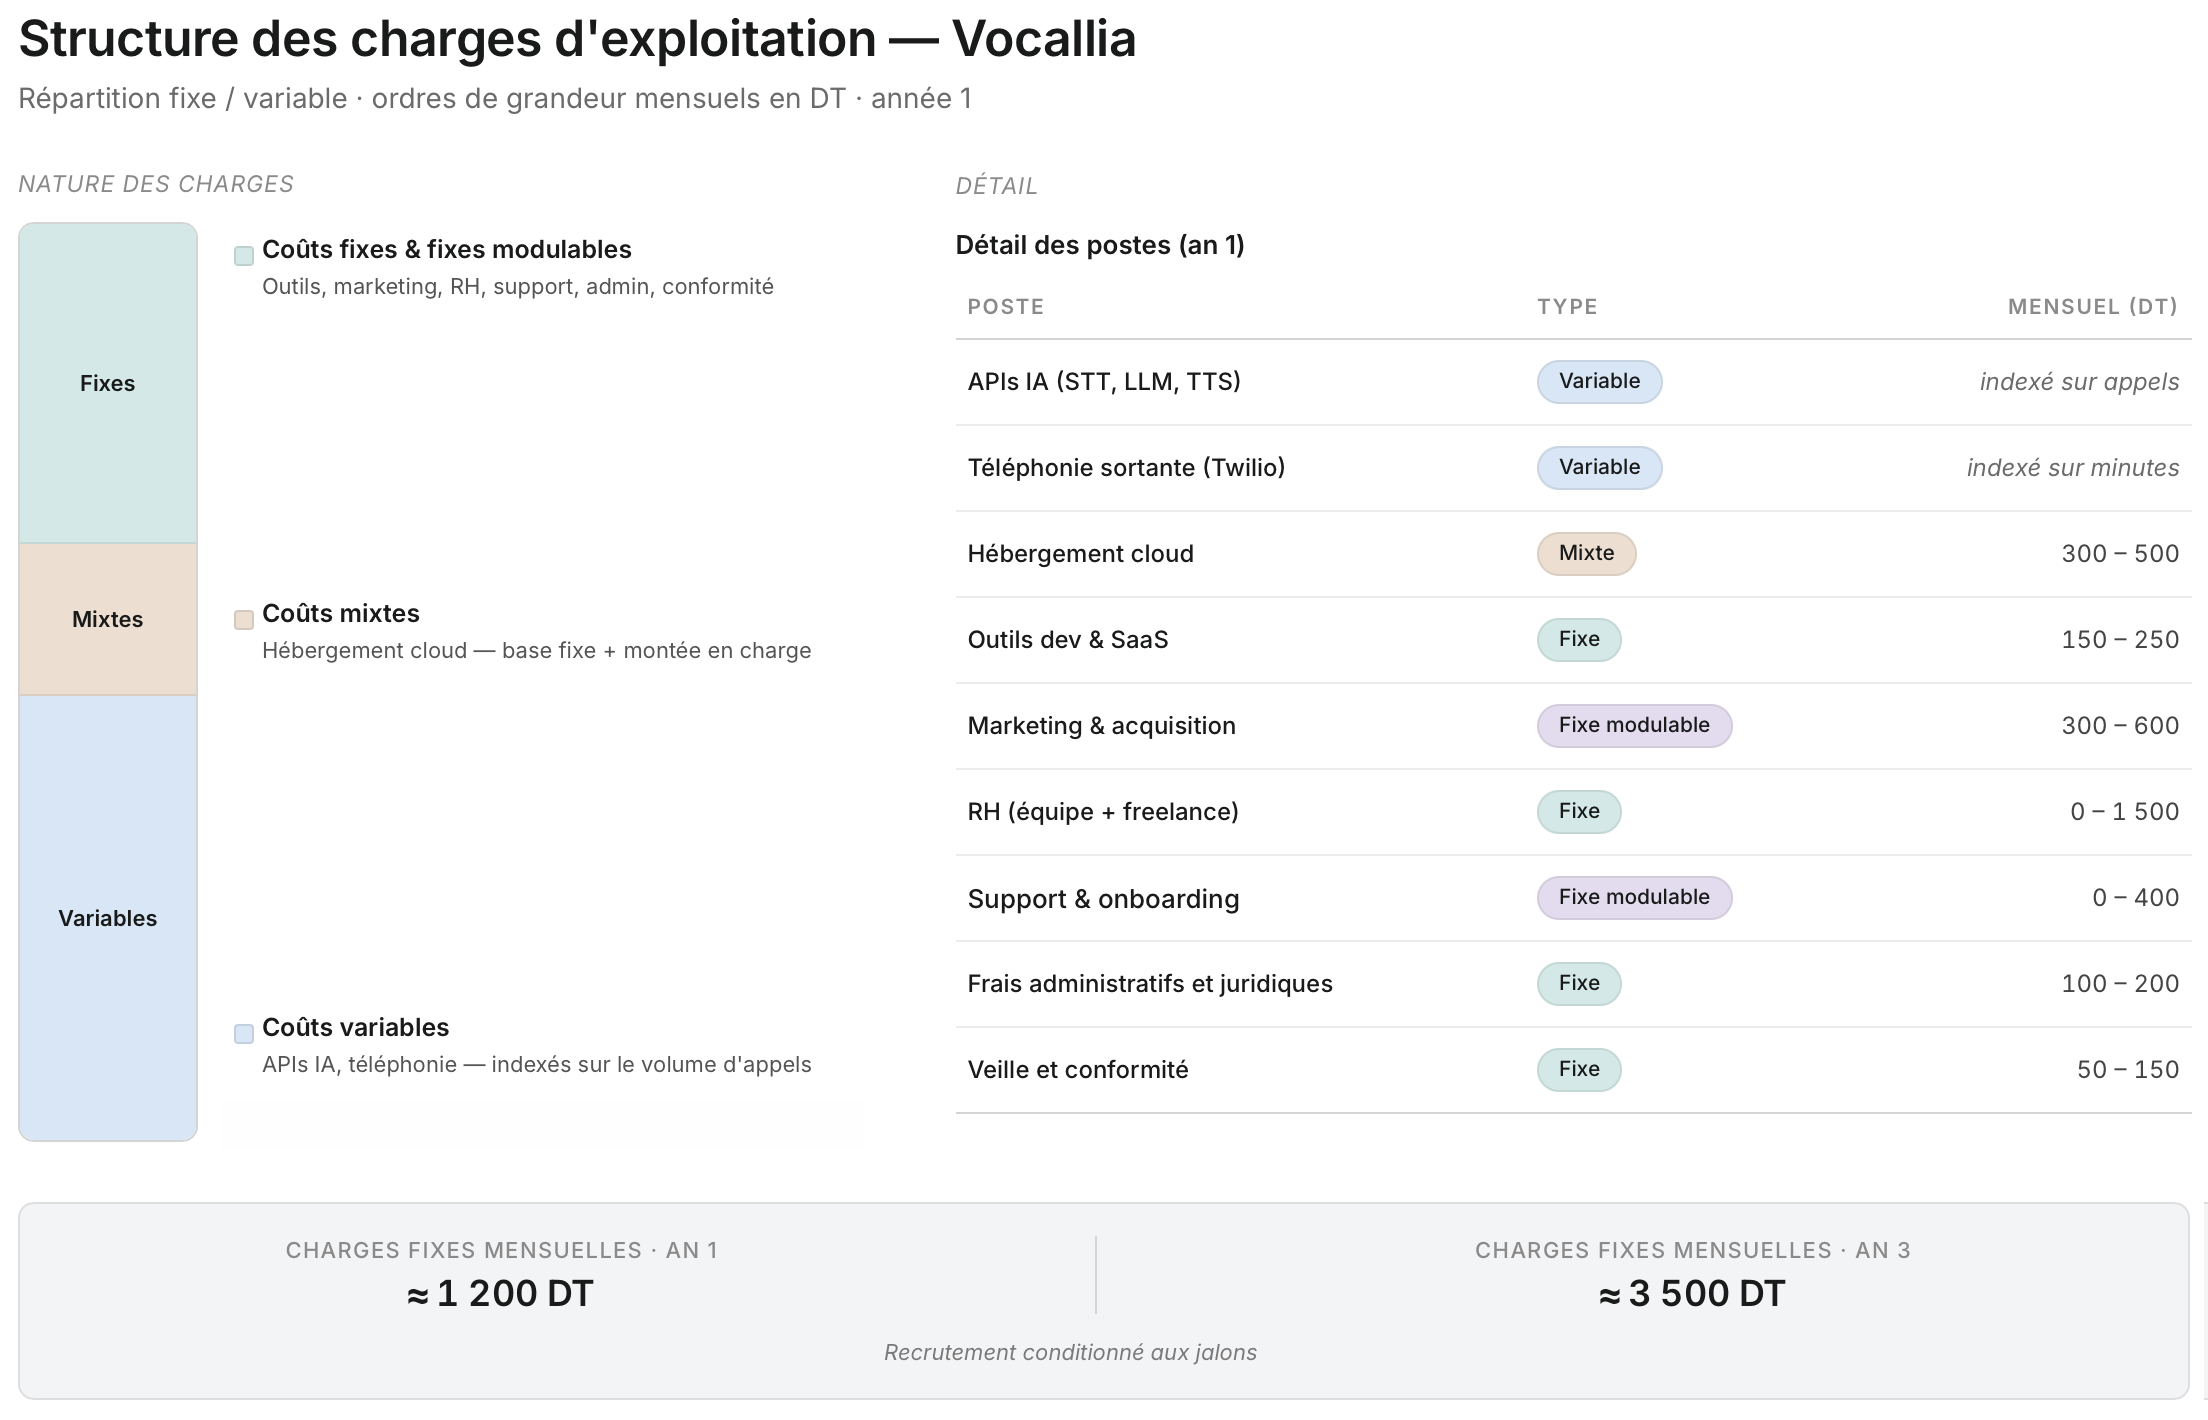
\includegraphics[width=\textwidth]{figures/structure-charges-exploitation-vocallia.png}
\caption{Structure des charges d'exploitation de Vocallia — répartition fixe / variable}
\label{fig:structure_charges}
\end{figure}

\begin{table}[H]
\centering
\caption{Structure des charges d'exploitation — Vocallia (en DT)}
\label{tab:charges_exploitation}
\begin{tabular}{|p{4cm}|p{2.5cm}|p{4cm}|p{4cm}|}
\hline
\textbf{Poste} & \textbf{Type} & \textbf{Ordre de grandeur mensuel (an~1)} & \textbf{Évolution attendue} \\
\hline
APIs IA (STT, LLM, TTS) & Variable & Indexé sur appels & Croît avec le volume, marge stable \\
\hline
Téléphonie sortante (Twilio) & Variable & Indexé sur minutes & Idem, négociable à l'échelle \\
\hline
Hébergement cloud (compute, stockage) & Mixte & 300 — 500 & Faible élasticité avant 200+ clients \\
\hline
Outils de développement et SaaS internes & Fixe & 150 — 250 & Stable \\
\hline
Marketing et acquisition (Meta Ads, SEO) & Fixe modulable & 300 — 600 & Augmente progressivement \\
\hline
Ressources humaines (équipe fondatrice + freelance) & Fixe & 0 — 1\,500 & Croissance conditionnée aux jalons \\
\hline
Support client et onboarding & Fixe modulable & 0 — 400 & À partir du mois~3 \\
\hline
Frais administratifs et juridiques & Fixe & 100 — 200 & Stable \\
\hline
Veille et conformité (INPDP, sécurité) & Fixe & 50 — 150 & Léger renforcement an~2 \\
\hline
\end{tabular}
\end{table}

\paragraph{Analyse de la structure.} Trois constats s'imposent. Les charges fixes mensuelles d'année~1 sont \textbf{volontairement contenues autour de 1\,200~DT}, niveau atteignable grâce à une équipe initiale réduite et à l'absence de loyer commercial. La part variable du coût total est \textbf{absorbée par la marge brute structurellement élevée} du plan Starter (de l'ordre de 65~\%, cf. chapitre~4)~: chaque appel facturé couvre largement son coût marginal. La hausse projetée des charges fixes en année~3 (vers 3\,500~DT/mois) est calibrée pour permettre un premier recrutement (commercial ou customer success) une fois le seuil de rentabilité opérationnel franchi — et non l'inverse. Cette discipline d'embauche conditionnée aux revenus est l'élément le plus important de la soutenabilité financière du modèle.

%%%%%%%%%%%%%%%%%%%%%%%%%%%%%%%%%%%%%%%%%%%%%%%%%%%%%%%%%%%%%%%%%%%%%%%%%%%
\section{Prévisions de chiffre d'affaires}
\label{sec:previsions_ca}
%%%%%%%%%%%%%%%%%%%%%%%%%%%%%%%%%%%%%%%%%%%%%%%%%%%%%%%%%%%%%%%%%%%%%%%%%%%

Le chiffre d'affaires de Vocallia est construit comme la somme de trois flux~: les abonnements mensuels récurrents (MRR), la facturation à l'usage des appels au-delà du forfait, et les frais ponctuels d'onboarding pour le palier Pro. Pour la projection, ces flux sont consolidés via un \textbf{ARPU pondéré} de l'ordre de 120~DT/mois, valeur cohérente avec un mix de portefeuille progressif Starter~$\to$~Croissance. La trajectoire du nombre de clients actifs prolonge directement les projections présentées au chapitre~3, en intégrant l'effet du churn mensuel et le rythme d'acquisition net.

\begin{table}[H]
\centering
\caption{Prévisions de chiffre d'affaires sur 3 ans — trois scénarios}
\label{tab:previsions_ca}
\begin{tabular}{|p{4cm}|p{3cm}|p{3cm}|p{3cm}|}
\hline
\textbf{Indicateur} & \textbf{Prudent} & \textbf{Central} & \textbf{Ambitieux} \\
\hline
\multicolumn{4}{|c|}{\textit{Année 1}} \\
\hline
Clients actifs (fin) & 20 & 40 & 65 \\
\hline
MRR fin d'année (DT) & $\sim$2\,400 & $\sim$4\,800 & $\sim$7\,800 \\
\hline
CA annuel (DT) & $\sim$22\,000 & $\sim$45\,000 & $\sim$72\,000 \\
\hline
\multicolumn{4}{|c|}{\textit{Année 2}} \\
\hline
Clients actifs (fin) & 35 & 70 & 120 \\
\hline
MRR fin d'année (DT) & $\sim$4\,200 & $\sim$8\,400 & $\sim$14\,400 \\
\hline
CA annuel (DT) & $\sim$40\,000 & $\sim$80\,000 & $\sim$140\,000 \\
\hline
\multicolumn{4}{|c|}{\textit{Année 3}} \\
\hline
Clients actifs (fin) & 50 & 100 & 180 \\
\hline
MRR fin d'année (DT) & $\sim$6\,000 & $\sim$12\,000 & $\sim$21\,600 \\
\hline
CA annuel (DT) & $\sim$60\,000 & $\sim$120\,000 & $\sim$220\,000 \\
\hline
\end{tabular}
\end{table}

\paragraph{Synthèse.} Ces projections sont délibérément conservatrices~: même le scénario ambitieux ne suppose qu'environ 5 nouveaux clients nets par mois en année~3, soit une dynamique modérée au regard de ce qui est généralement observé pour les SaaS B2B ayant atteint la traction \emph{product-market fit}. Le scénario prudent, lui, est calibré pour que le projet reste vivant même dans une configuration de croissance lente — propriété essentielle pour une thèse d'investissement défendable. Ces trajectoires restent toutefois des projections~: elles seront recalibrées à la lumière des données réelles d'acquisition et de churn observées en phase pilote.

%%%%%%%%%%%%%%%%%%%%%%%%%%%%%%%%%%%%%%%%%%%%%%%%%%%%%%%%%%%%%%%%%%%%%%%%%%%
\section{Compte de résultat prévisionnel}
\label{sec:compte_resultat}
%%%%%%%%%%%%%%%%%%%%%%%%%%%%%%%%%%%%%%%%%%%%%%%%%%%%%%%%%%%%%%%%%%%%%%%%%%%

Le compte de résultat prévisionnel agrège les hypothèses de revenus et de charges précédentes pour produire une estimation lisible de la marge brute et du résultat opérationnel sur 36~mois. Il est présenté ici dans le scénario central, considéré comme le plus probable. La figure~\ref{fig:projection_36_mois} en représente la trajectoire visuelle~: revenus, coûts variables, charges fixes et résultat opérationnel sur l'horizon complet de projection.

\begin{figure}[H]
\centering
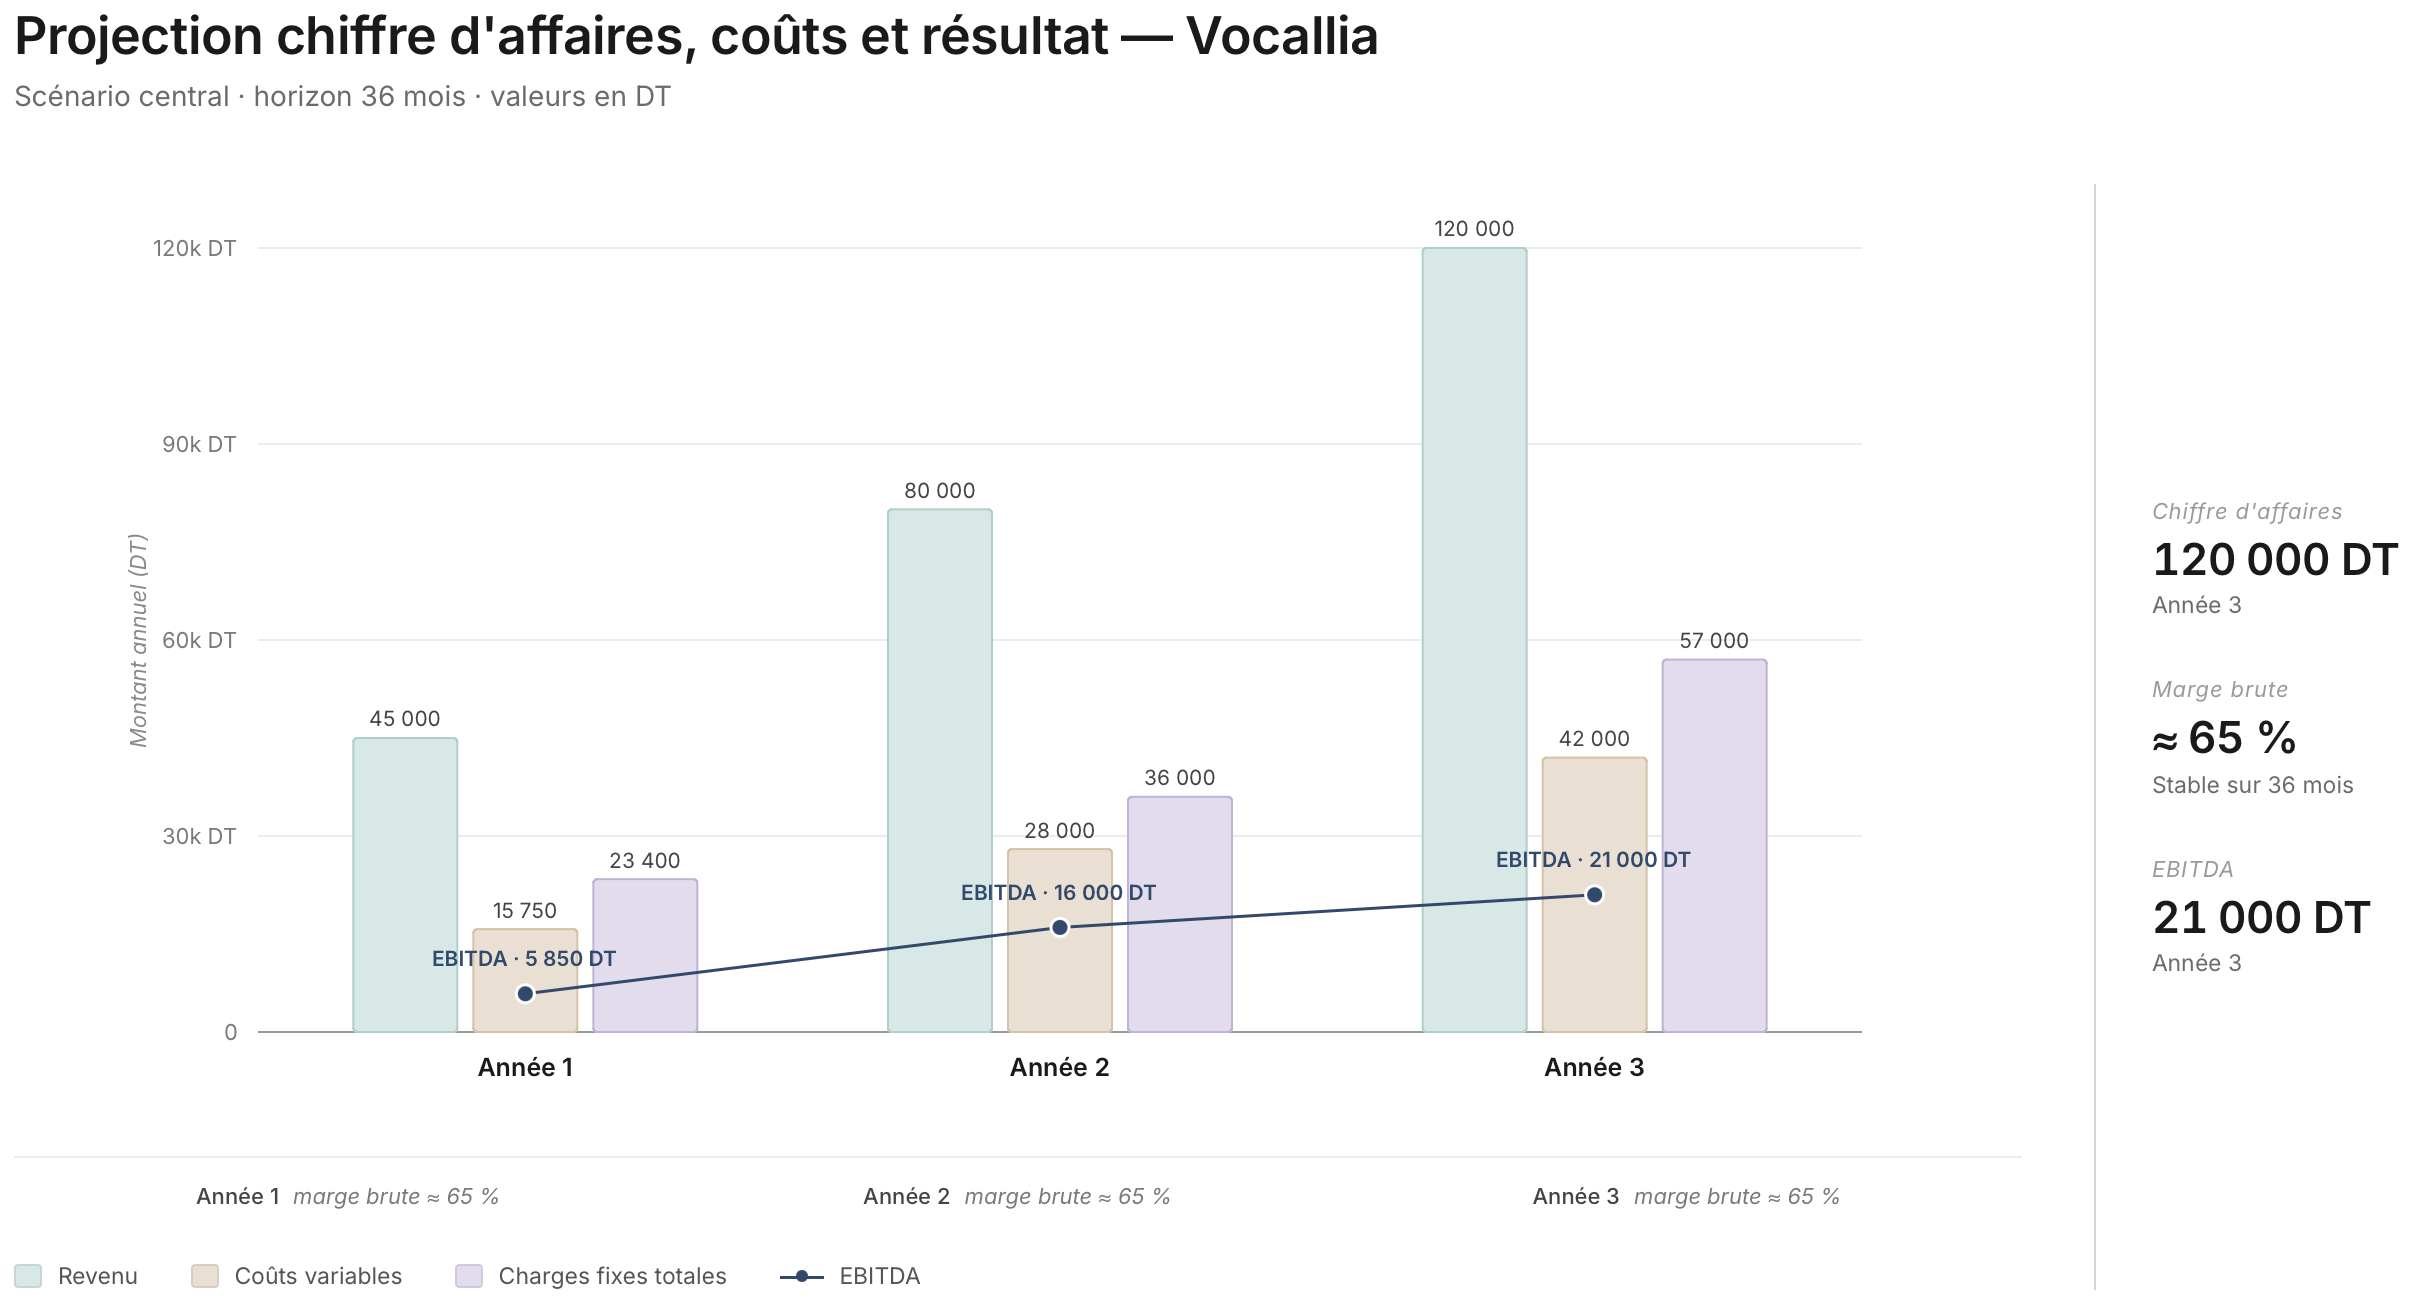
\includegraphics[width=\textwidth]{figures/projection-ca-couts-resultat-36-mois.png}
\caption{Projection chiffre d'affaires, coûts et résultat opérationnel sur 36 mois — scénario central}
\label{fig:projection_36_mois}
\end{figure}

\begin{table}[H]
\centering
\caption{Compte de résultat prévisionnel — scénario central (en DT)}
\label{tab:compte_resultat}
\begin{tabular}{|p{5cm}|p{3cm}|p{3cm}|p{3cm}|}
\hline
\textbf{Poste} & \textbf{Année 1} & \textbf{Année 2} & \textbf{Année 3} \\
\hline
Chiffre d'affaires & $\sim$45\,000 & $\sim$80\,000 & $\sim$120\,000 \\
\hline
Coûts variables (APIs, téléphonie, hébergement marginal) & $\sim$15\,750 & $\sim$28\,000 & $\sim$42\,000 \\
\hline
\textbf{Marge brute} & $\sim$29\,250 & $\sim$52\,000 & $\sim$78\,000 \\
\hline
Charges fixes opérationnelles & $\sim$14\,400 & $\sim$24\,000 & $\sim$42\,000 \\
\hline
Charges marketing et acquisition & $\sim$6\,000 & $\sim$8\,000 & $\sim$10\,000 \\
\hline
Charges administratives et conformité & $\sim$3\,000 & $\sim$4\,000 & $\sim$5\,000 \\
\hline
\textbf{Résultat opérationnel (EBITDA)} & $\sim$\,5\,850 & $\sim$16\,000 & $\sim$21\,000 \\
\hline
Amortissement de l'investissement initial & $\sim$6\,000 & $\sim$6\,000 & $\sim$6\,000 \\
\hline
\textbf{Résultat avant impôt} & $\sim$\,-150 & $\sim$10\,000 & $\sim$15\,000 \\
\hline
Impôts (régime Startup Act) & 0 — exonéré & 0 — exonéré & 0 — exonéré \\
\hline
\textbf{Résultat net estimé} & $\sim$\,-150 & $\sim$10\,000 & $\sim$15\,000 \\
\hline
\end{tabular}
\end{table}

\paragraph{Lecture analytique.} Le scénario central fait apparaître trois enseignements, qu'il convient de présenter avec prudence. D'abord, une marge brute structurellement élevée, qui reflète la dominance des coûts variables et la soutenabilité économique du palier Starter démontrée au chapitre~4. Ensuite, un \textbf{EBITDA légèrement positif dès la première année dans le scénario central}, soutenu par la modération volontaire des charges fixes — résultat conditionné au respect strict de la trajectoire d'acquisition et à la maîtrise des charges fixes. Enfin, un résultat net proche de l'équilibre en année~1 puis modérément positif en années~2 et~3, sous réserve que la trajectoire d'acquisition projetée soit effectivement tenue. En scénario prudent, le résultat net resterait négatif en années~1 et~2 et tendrait vers l'équilibre en année~3~; en scénario ambitieux, l'équilibre serait atteint plus tôt. Ces estimations doivent être lues comme des ordres de grandeur et non comme des engagements de performance.

%%%%%%%%%%%%%%%%%%%%%%%%%%%%%%%%%%%%%%%%%%%%%%%%%%%%%%%%%%%%%%%%%%%%%%%%%%%
\section{Seuil de rentabilité et analyse du point mort}
\label{sec:seuil_rentabilite}
%%%%%%%%%%%%%%%%%%%%%%%%%%%%%%%%%%%%%%%%%%%%%%%%%%%%%%%%%%%%%%%%%%%%%%%%%%%

\subsection{Méthodologie et calcul du point mort}
\label{subsec:methodo_seuil}

Le seuil de rentabilité opérationnel est défini comme le niveau de chiffre d'affaires — et donc de clients actifs — à partir duquel la marge brute couvre intégralement les charges fixes opérationnelles. Avec un ARPU pondéré d'environ 120~DT/mois et une marge brute de l'ordre de 65~\%, chaque client actif contribue à hauteur d'environ \textbf{78~DT/mois} à la couverture des charges fixes. Il s'agit ici d'un seuil de rentabilité \emph{opérationnel}, hors amortissement de l'investissement initial.

En appliquant cette contribution unitaire aux charges fixes mensuelles projetées, on obtient les seuils synthétisés dans le tableau~\ref{tab:seuil_rentabilite}, dont la figure~\ref{fig:seuil_rentabilite} fournit la lecture visuelle.

\begin{table}[H]
\centering
\caption{Seuil de rentabilité opérationnelle — Vocallia}
\label{tab:seuil_rentabilite}
\begin{tabular}{|p{3cm}|p{3.5cm}|p{4cm}|p{3.5cm}|}
\hline
\textbf{Année} & \textbf{Charges fixes mensuelles (DT)} & \textbf{Contribution par client (DT/mois)} & \textbf{Clients actifs au point mort} \\
\hline
Année 1 & $\sim$1\,200 & $\sim$78 & $\sim$15 — 16 \\
\hline
Année 2 & $\sim$2\,000 & $\sim$78 & $\sim$25 — 27 \\
\hline
Année 3 & $\sim$3\,500 & $\sim$78 & $\sim$45 \\
\hline
\end{tabular}
\end{table}

\begin{figure}[H]
\centering
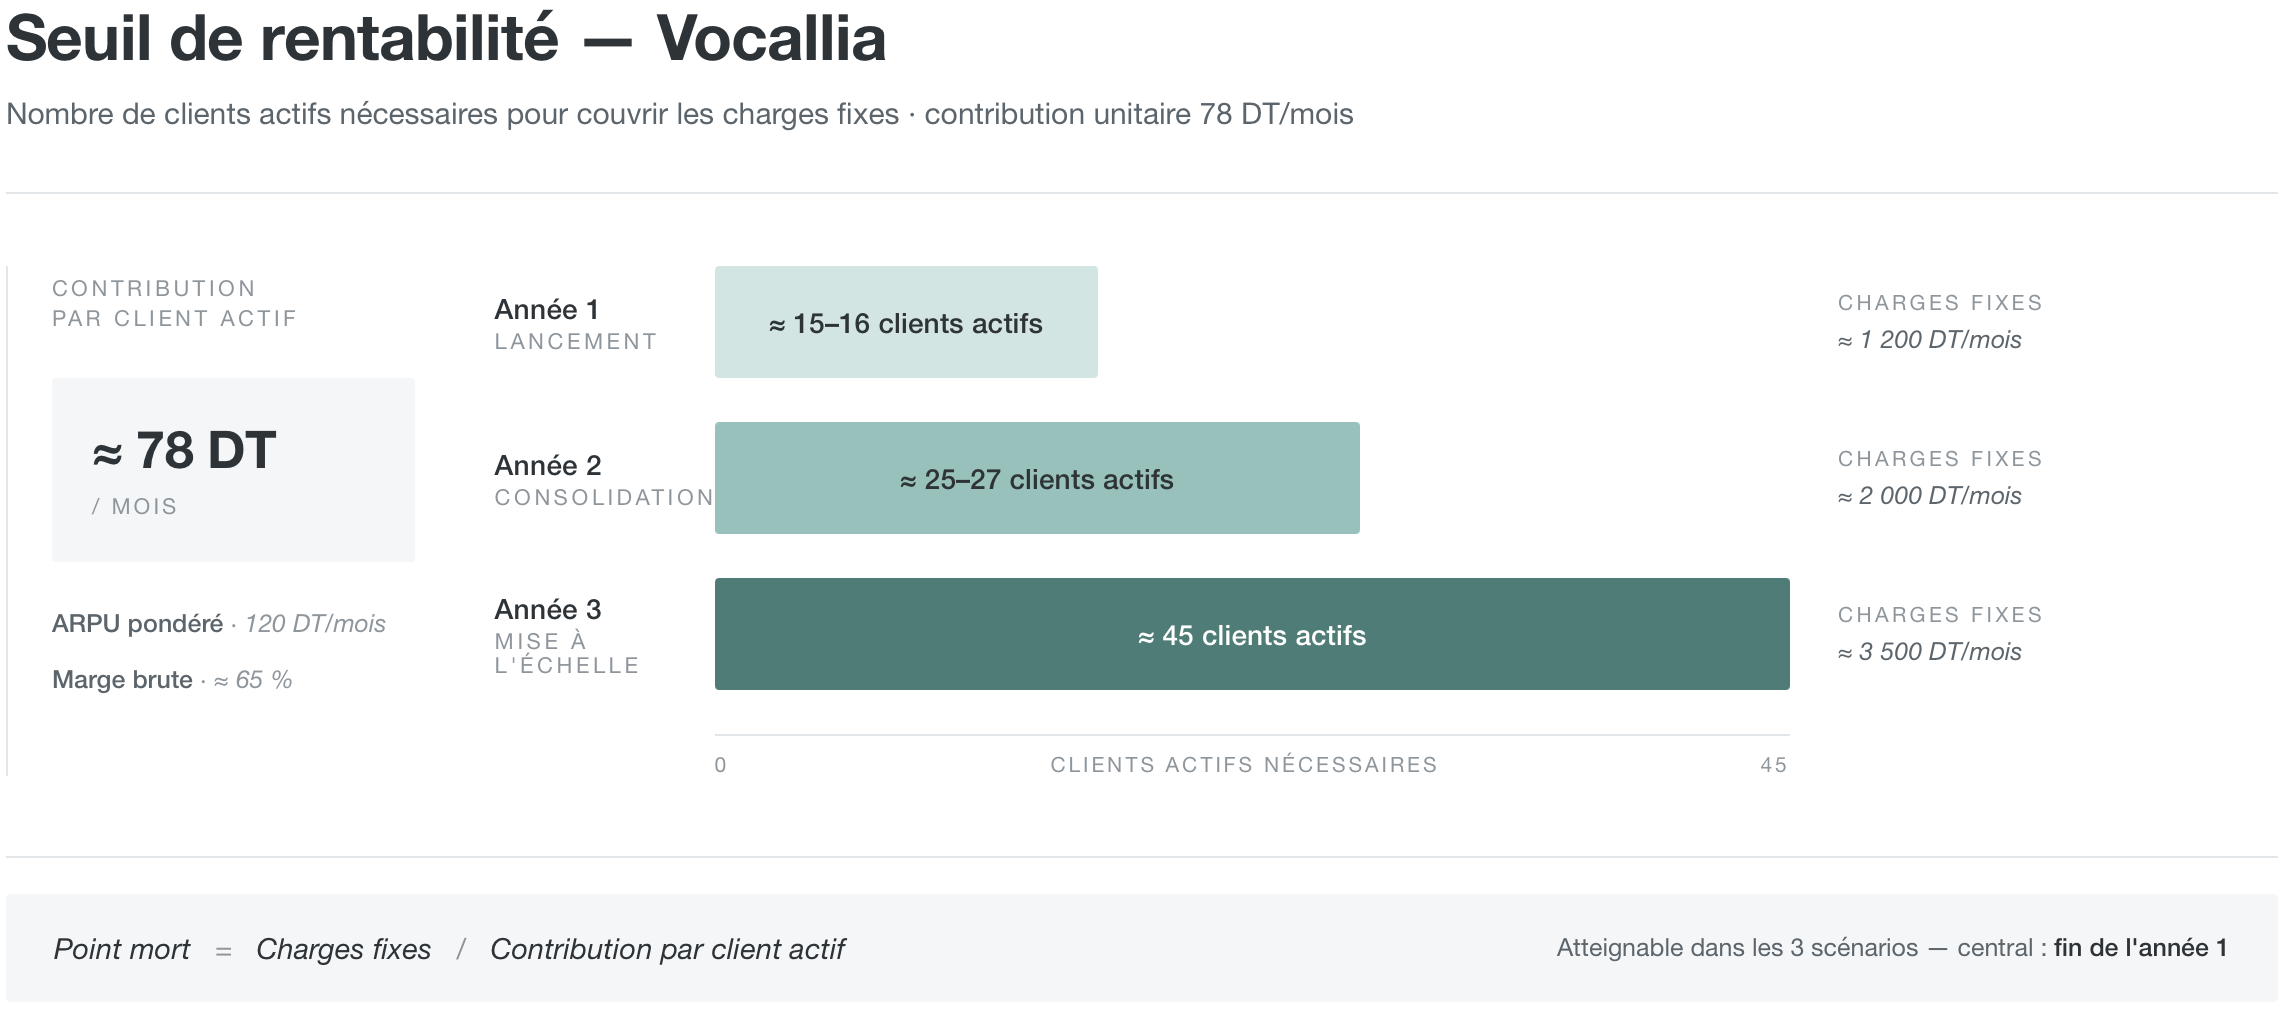
\includegraphics[width=\textwidth]{figures/seuil-rentabilite-clients-actifs.png}
\caption{Seuil de rentabilité — clients actifs nécessaires par année}
\label{fig:seuil_rentabilite}
\end{figure}

\begin{quote}
\textbf{Lecture stratégique.} Le seuil opérationnel apparaît atteignable dans tous les scénarios sous réserve de tenue de la trajectoire commerciale~: vers la fin du mois~12 dans le scénario central, plus tôt dans le scénario ambitieux, en cours d'année~3 dans le scénario prudent. Cette propriété est précisément le résultat de la discipline d'architecture frugale du chapitre~4 et du modèle PLG du chapitre~3~: en limitant volontairement les charges fixes en phase d'amorçage, Vocallia rend son point mort opérationnel accessible avec un nombre de clients qui correspond à la borne basse crédible des projections commerciales. Il convient toutefois de rappeler que ce seuil ne couvre pas l'amortissement de l'investissement initial, qui exigera une période plus longue pour être pleinement absorbé.
\end{quote}

\subsection{Sensibilité du point mort}
\label{subsec:sensibilite_seuil}

Trois variables affectent directement la trajectoire du point mort. Une \textbf{hausse de 20~\%} des coûts API (volatilité tarifaire) réduirait la marge brute d'environ 6~points et augmenterait le seuil de quelques clients seulement — sensibilité faible. Une \textbf{augmentation de 50~\%} des charges fixes (par exemple un recrutement anticipé) repousserait le point mort de 7 à 8 clients — sensibilité moyenne. Un \textbf{churn dégradé à 10~\%/mois} éroderait la LTV et exigerait un rythme d'acquisition brut sensiblement supérieur pour maintenir le même nombre de clients actifs nets — sensibilité élevée. Le churn est donc le levier le plus critique~: c'est lui qui doit faire l'objet de la surveillance la plus attentive en phase d'exécution.

%%%%%%%%%%%%%%%%%%%%%%%%%%%%%%%%%%%%%%%%%%%%%%%%%%%%%%%%%%%%%%%%%%%%%%%%%%%
\section{Plan de financement}
\label{sec:plan_financement}
%%%%%%%%%%%%%%%%%%%%%%%%%%%%%%%%%%%%%%%%%%%%%%%%%%%%%%%%%%%%%%%%%%%%%%%%%%%

La philosophie de financement retenue est résolument \textbf{progressive et non dilutive en priorité}. Plutôt que de lever un capital important en phase prématurée — ce qui imposerait une dilution significative et une pression de croissance disproportionnée — Vocallia structure son financement en couches superposées, chacune activée lorsque la précédente est consommée et que les jalons associés sont franchis. La figure~\ref{fig:plan_financement} en illustre le séquencement.

\begin{figure}[H]
\centering
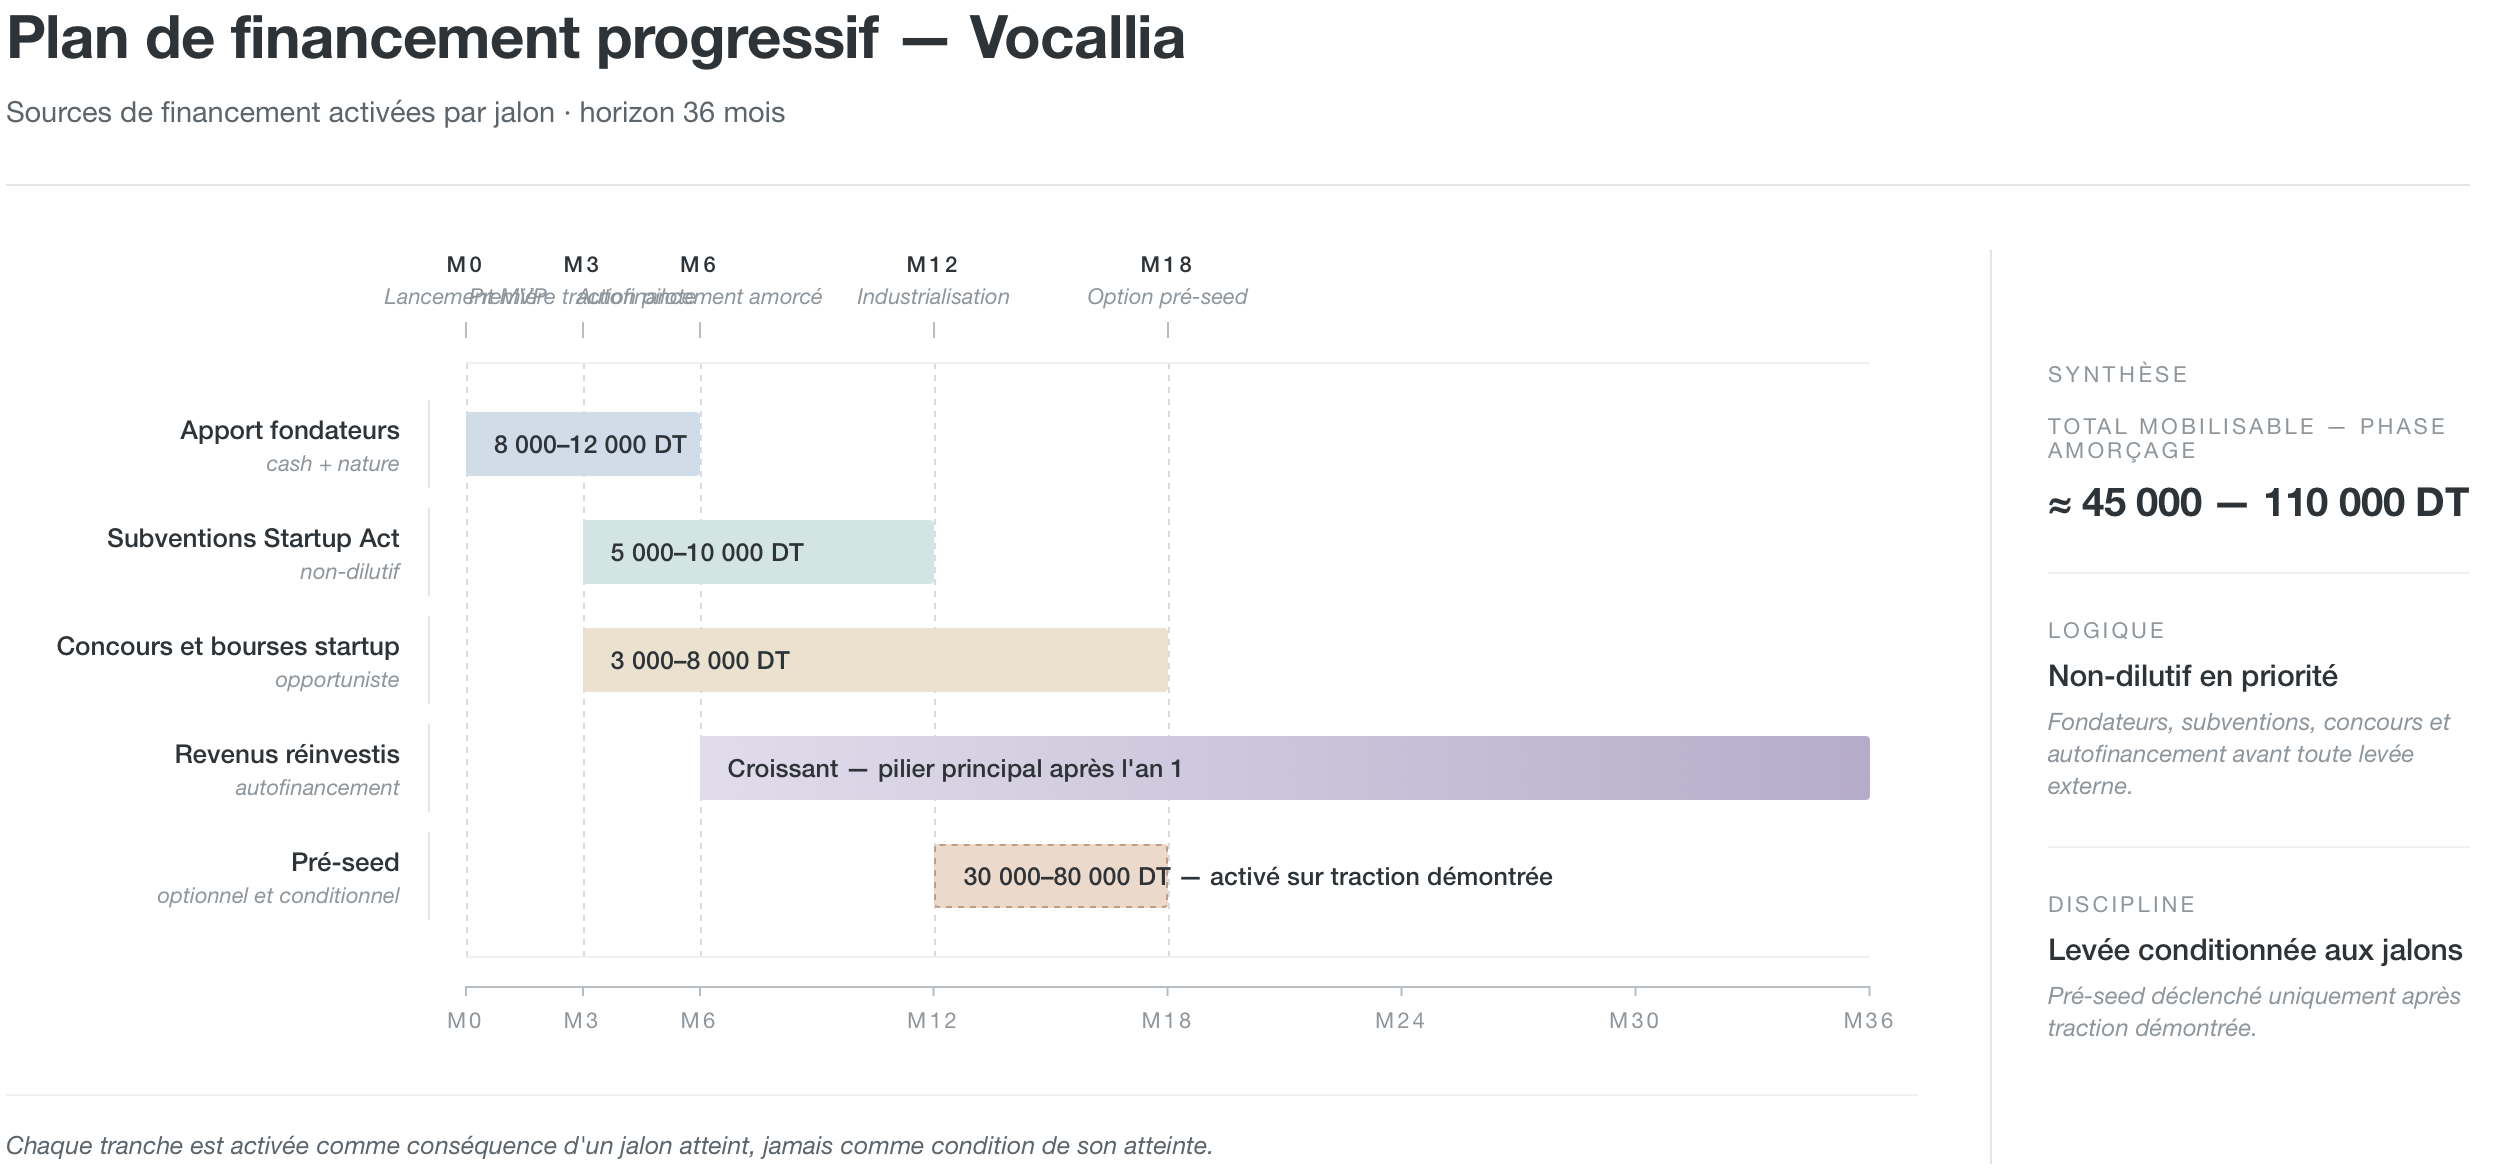
\includegraphics[width=\textwidth]{figures/plan-financement-progressif-vocallia.png}
\caption{Plan de financement progressif de Vocallia — sources et activation par jalon}
\label{fig:plan_financement}
\end{figure}

\begin{table}[H]
\centering
\caption{Plan de financement structuré — Vocallia (horizon 36 mois)}
\label{tab:plan_financement}
\begin{tabular}{|p{4cm}|p{3cm}|p{3cm}|p{4cm}|}
\hline
\textbf{Source} & \textbf{Montant cible (DT)} & \textbf{Horizon} & \textbf{Conditions / logique} \\
\hline
Apport fondateurs (cash + nature) & 8\,000 — 12\,000 & Mois~0 & Développement MVP, premiers tests \\
\hline
Subventions et appuis Startup Act & 5\,000 — 10\,000 & Mois~3 — Mois~12 & Labellisation, BFG, primes mensuelles \\
\hline
Concours et bourses startup & 3\,000 — 8\,000 & Mois~3 — Mois~18 & Conditionné à la traction démontrée \\
\hline
Revenus réinvestis (autofinancement) & Croissant & À partir du mois~6 & Pilier principal après l'an~1 \\
\hline
Pré-seed potentiel (optionnel) & 30\,000 — 80\,000 & Mois~12 — Mois~18 & Activé seulement si trajectoire ambitieuse \\
\hline
\textbf{Total mobilisable phase amorçage} & \textbf{$\sim$45\,000 — 110\,000} & — & Modulé selon scénario \\
\hline
\end{tabular}
\end{table}

\paragraph{Justification du séquençage.} Trois raisons fondent ce séquençage. Le \textbf{Startup Act} (loi n°2018-20) offre un dispositif particulièrement avantageux dont l'activation précoce — labellisation dès la phase MVP — peut débloquer exonérations fiscales, accès devises et primes mensuelles, sans dilution. Le modèle économique permet une \textbf{contribution progressive de l'autofinancement à partir du mois~6}, dans la mesure où la marge brute couvre déjà à ce stade une part des charges fixes~: chaque client actif réduit alors progressivement la dépendance aux financements externes pour les charges courantes. Le recours à un \textbf{tour pré-seed} n'est envisagé que de manière conditionnelle, lorsqu'une traction documentée (15 à 25 clients actifs payants, MRR autour de 3\,000~DT, churn maîtrisé) permet de négocier des conditions favorables — situation très différente d'une levée prématurée.

\begin{quote}
\textbf{Discipline de financement.} Lever trop tôt est l'un des risques les plus sous-estimés des startups SaaS d'amorçage~: cela impose des objectifs de croissance déconnectés des fondamentaux du produit. Vocallia inverse délibérément cette logique~: chaque tranche de financement est activée comme conséquence d'un jalon atteint, et non comme condition préalable de son atteinte.
\end{quote}

%%%%%%%%%%%%%%%%%%%%%%%%%%%%%%%%%%%%%%%%%%%%%%%%%%%%%%%%%%%%%%%%%%%%%%%%%%%
\section{Indicateurs de rentabilité}
\label{sec:indicateurs_rentabilite}
%%%%%%%%%%%%%%%%%%%%%%%%%%%%%%%%%%%%%%%%%%%%%%%%%%%%%%%%%%%%%%%%%%%%%%%%%%%

\subsection{Approche méthodologique et précautions}
\label{subsec:methodo_indicateurs}

Calculer une VAN ou un TRI rigoureux à ce stade exigerait des hypothèses précises sur le taux d'actualisation, la structure de capital, la valeur terminale et la durée d'extrapolation, dont aucune n'est aujourd'hui suffisamment stabilisée pour produire un chiffre défendable au centième près. Plutôt que d'inventer une fausse précision, ce chapitre présente un \textbf{cadre indicatif} fondé sur les flux du scénario central, en identifiant clairement les paramètres qui devront être affinés à l'issue de la phase pilote.

\subsection{Indicateurs estimés}
\label{subsec:indicateurs_estimes}

\paragraph{Période de retour estimée de l'investissement initial.} Avec un investissement initial estimé autour de 25\,000~DT et un EBITDA cumulé estimé d'environ 42\,000~DT sur 3~ans en scénario central, l'investissement initial pourrait, en première approche, être absorbé entre la fin de l'année~2 et le milieu de l'année~3, soit une période de retour indicative \textbf{de l'ordre de 24 à 30 mois}. Cette estimation suppose toutefois que l'EBITDA généré soit intégralement disponible pour absorber l'investissement initial, ce qui ne tient pas compte d'éventuels besoins en fonds de roulement ou réinvestissements produit qui pourraient l'allonger. Cette durée reste néanmoins cohérente avec ce qui est généralement attendu sur les SaaS B2B en phase d'amorçage.

\paragraph{Cash-flow opérationnel et cash-flow cumulé.} Il convient de distinguer deux notions souvent confondues. Le \textbf{cash-flow opérationnel} (généré par l'exploitation courante hors investissement initial) pourrait devenir légèrement positif dès la fin de l'année~1 dans le scénario central, dans la continuité du résultat opérationnel projeté. Le \textbf{cash-flow cumulé} (intégrant l'investissement initial de l'ordre de 25\,000~DT) resterait en revanche négatif sur la majeure partie de l'horizon~: il devrait progressivement converger vers l'équilibre au cours de l'année~2 dans le scénario central, et n'atteindrait une trajectoire franchement positive qu'en année~3. En scénario prudent, le cash-flow cumulé resterait négatif plus longtemps, ce qui justifie la mobilisation des subventions et concours en complément.

\paragraph{LTV/CAC et CAC payback — cadre indicatif.} Comme indiqué au chapitre~3, le ratio LTV/CAC visé se situe au-dessus du seuil minimal de 3~:~1 généralement attendu par les investisseurs SaaS, et le CAC payback est ciblé en deçà de 6~mois. Ces ratios reposent toutefois sur des hypothèses de churn, d'ARPU et de coût d'acquisition qui devront être confirmées par les données réelles de la phase pilote. À ce stade, le CPL de l'ordre de 0{,}36~euro observé pendant la phase Muvaka constitue un signal favorable de génération de leads, mais ne préjuge pas du coût d'acquisition client effectif, qui dépendra du taux de conversion observé une fois le pilote engagé.

\paragraph{VAN et TRI — cadre indicatif.} À titre purement indicatif, et sous réserve de stabilisation des hypothèses, une projection à 5~ans avec un taux d'actualisation de l'ordre de 15~\% (cohérent avec un risque pays / risque early-stage en zone MENA) ferait apparaître une VAN potentiellement positive en scénario central, sous l'hypothèse explicite que la trajectoire d'acquisition soit prolongée au-delà de l'horizon de 36~mois et que les hypothèses de marge soient confirmées. Le TRI ne peut pas être chiffré de manière crédible avant l'achèvement de la phase pilote, qui fournira les données réelles d'acquisition, de churn et d'expansion nécessaires. Ces deux indicateurs doivent donc être présentés ici comme un \emph{cadre méthodologique}, et non comme des résultats de calcul.

%%%%%%%%%%%%%%%%%%%%%%%%%%%%%%%%%%%%%%%%%%%%%%%%%%%%%%%%%%%%%%%%%%%%%%%%%%%
\section{Plan d'exécution opérationnelle}
\label{sec:plan_execution}
%%%%%%%%%%%%%%%%%%%%%%%%%%%%%%%%%%%%%%%%%%%%%%%%%%%%%%%%%%%%%%%%%%%%%%%%%%%

Le plan d'exécution opérationnelle articule en quatre phases la transformation du projet en activité économique pérenne. Il croise quatre familles de jalons~: \textbf{technique} (cf.~chapitre~4), \textbf{commercial} (cf.~chapitre~3), \textbf{financier} (présent chapitre) et \textbf{réglementaire} (engagement INPDP, labellisation Startup Act). La figure~\ref{fig:roadmap_execution} en propose une représentation séquentielle.

\begin{figure}[H]
\centering
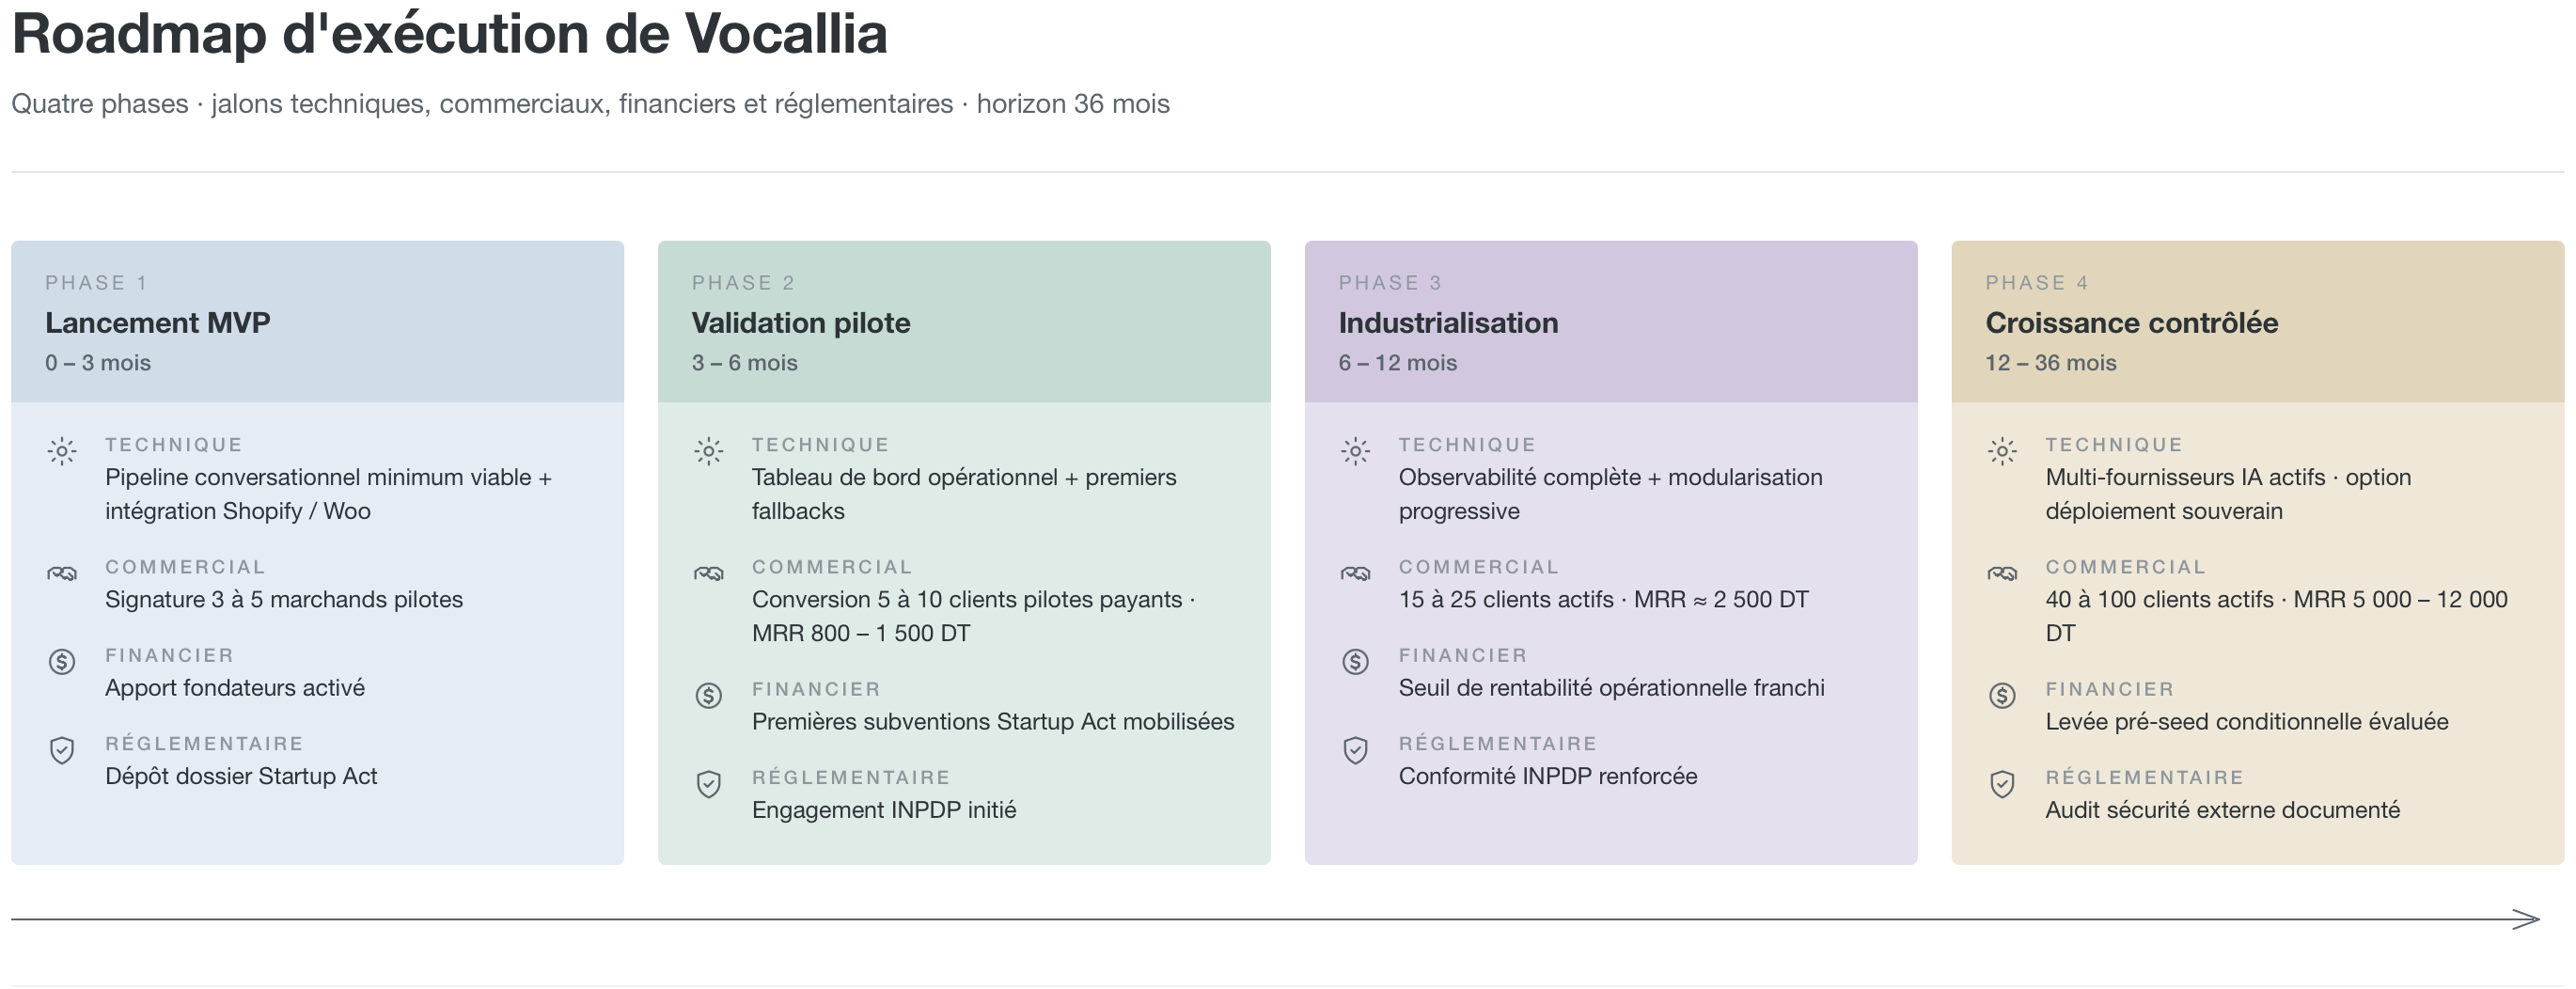
\includegraphics[width=\textwidth]{figures/roadmap-execution-vocallia.png}
\caption{Roadmap d'exécution de Vocallia — du MVP à la production (0--36 mois)}
\label{fig:roadmap_execution}
\end{figure}

\subsection{Phase 0--3 mois — Lancement du MVP}
\label{subsec:phase_0_3}

L'objectif est de mettre en service un MVP fonctionnel intégré à une plateforme e-commerce et utilisable par 1 à 3 marchands pilotes. Jalons critiques~: livraison du pipeline conversationnel minimum viable, mise en place du tableau de bord et des intégrations de base, dépôt du dossier Startup Act, lancement des premières campagnes Meta Ads, signature des 3 à 5 premiers pilotes.

\subsection{Phase 3--6 mois — Validation pilote}
\label{subsec:phase_3_6}

Le pilote vise à transformer les premiers utilisateurs gratuits en clients payants, en démontrant la valeur économique mesurable côté marchand. Jalons~: conversion de 5 à 10 clients pilotes en abonnements payants, atteinte d'un MRR de 800 à 1\,500~DT, premier rapport mensuel automatisé livré, engagement INPDP initié, premier témoignage client publié.

\subsection{Phase 6--12 mois — Industrialisation}
\label{subsec:phase_6_12}

L'objectif est de stabiliser le produit en production, viser le seuil de rentabilité opérationnelle et structurer les processus commerciaux et techniques. Jalons~: 15 à 25 clients actifs en scénario central, MRR autour de 2\,500~DT, mise en place de l'observabilité complète, modularisation progressive de l'architecture, premier recrutement freelance customer success conditionné au seuil franchi, lancement du programme de parrainage.

\subsection{Phase 12--36 mois — Croissance contrôlée}
\label{subsec:phase_12_36}

La trajectoire de moyen terme combine élargissement vertical (relance après abandon, prise de RDV, qualification de leads) et densification horizontale (acquisition de nouveaux marchands e-commerce). Jalons~: 40 à 100 clients actifs en scénario central, MRR entre 5\,000 et 12\,000~DT, premier recrutement permanent (commercial), évaluation conditionnelle d'une levée pré-seed, déploiement éventuel de l'option d'hébergement souverain pour comptes institutionnels.

\paragraph{Synthèse.} La séquence est calibrée pour que chaque investissement (recrutement, levée, expansion sectorielle) soit la \emph{conséquence} d'un jalon atteint, jamais sa \emph{condition} de financement. C'est précisément ce qui distingue un plan d'exécution discipliné d'un plan d'exécution optimiste.

%%%%%%%%%%%%%%%%%%%%%%%%%%%%%%%%%%%%%%%%%%%%%%%%%%%%%%%%%%%%%%%%%%%%%%%%%%%
\section{Impact économique et social}
\label{sec:impact_economique_social}
%%%%%%%%%%%%%%%%%%%%%%%%%%%%%%%%%%%%%%%%%%%%%%%%%%%%%%%%%%%%%%%%%%%%%%%%%%%

L'impact attendu de Vocallia dépasse la stricte performance financière de l'entreprise. Cinq dimensions méritent d'être explicitées, dans la continuité de l'analyse PESTEL conduite au chapitre~2.

\paragraph{Réduction des pertes pour l'écosystème e-commerce tunisien.} En contribuant à diminuer le taux de retours non anticipés et de ventes perdues faute de joignabilité, Vocallia peut produire un effet d'économie agrégée pour les marchands~: à l'échelle de quelques dizaines de PME équipées, les économies cumulées sur les coûts logistiques et le temps opérationnel libéré atteindraient des ordres de grandeur significatifs au regard de la taille du marché.

\paragraph{Gains de productivité et formalisation des opérations.} Pour le marchand, la confirmation automatisée pourrait libérer une part notable du temps gérant — capital humain réinjecté dans des tâches à plus forte valeur (croissance, achats, expérience client). Au-delà du gain individuel, le tableau de bord et les rapports mensuels participent d'une \textbf{formalisation progressive} des opérations e-commerce locales, contribution non négligeable à la professionnalisation du secteur.

\paragraph{Soutien à l'entrepreneuriat numérique tunisien.} Vocallia s'inscrit dans la dynamique du Startup Act et participe à l'émergence d'une nouvelle génération de startups SaaS tunisiennes développant des produits adaptés au contexte local — par opposition à une logique de simple intégration de solutions étrangères.

\paragraph{Création potentielle d'emplois qualifiés.} Au-delà du noyau fondateur, la trajectoire prévoit un premier recrutement en année~2 (customer success ou commercial), puis l'élargissement progressif de l'équipe, conditionné à l'atteinte des jalons financiers. L'écosystème d'intégrateurs, de consultants et de partenaires commerciaux pourrait également générer des opportunités indirectes.

\paragraph{Renforcement des capacités locales en IA appliquée.} Le corpus dialectal propriétaire que Vocallia construit progressivement constitue, à terme, un actif d'intérêt stratégique pour la communauté technologique locale~: il documente le darija dans un format exploitable par d'autres applications (santé, services publics, éducation) et représente un ancrage concret du développement de l'IA appliquée au contexte tunisien.

%%%%%%%%%%%%%%%%%%%%%%%%%%%%%%%%%%%%%%%%%%%%%%%%%%%%%%%%%%%%%%%%%%%%%%%%%%%
\section{Analyse des risques financiers et opérationnels}
\label{sec:risques_financiers}
%%%%%%%%%%%%%%%%%%%%%%%%%%%%%%%%%%%%%%%%%%%%%%%%%%%%%%%%%%%%%%%%%%%%%%%%%%%

Aucun plan financier ne tient sans une cartographie lucide de ses risques. Vocallia identifie huit risques principaux, classés selon leur probabilité et leur impact, et associe à chacun une mesure de mitigation directement opérationnelle. La figure~\ref{fig:matrice_risques} en propose une représentation matricielle.

\begin{figure}[H]
\centering
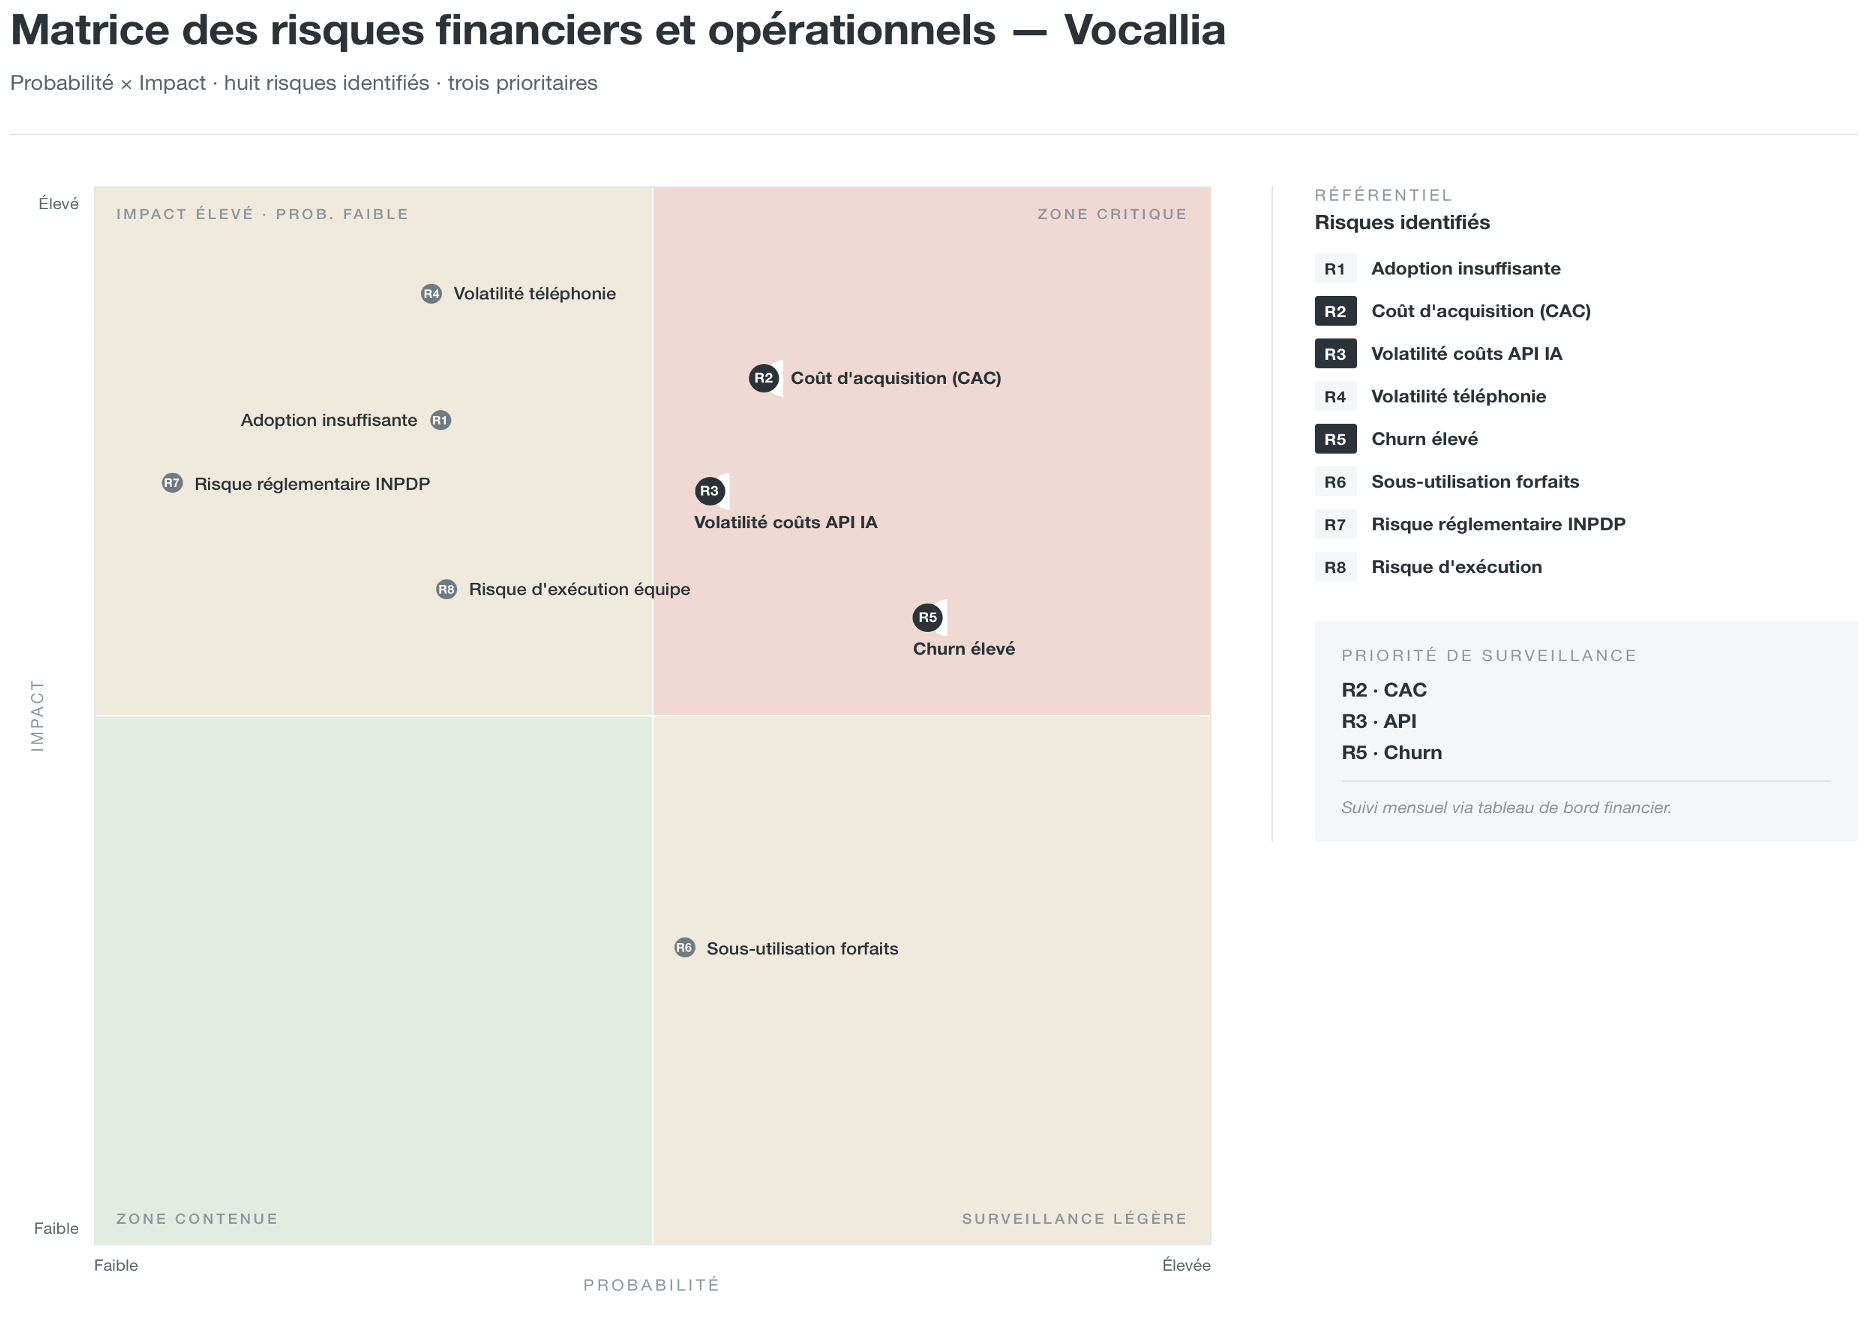
\includegraphics[width=\textwidth]{figures/matrice-risques-financiers-vocallia.png}
\caption{Matrice des risques financiers et opérationnels — Vocallia}
\label{fig:matrice_risques}
\end{figure}

\begin{table}[H]
\centering
\caption{Risques financiers et opérationnels — mesures de mitigation}
\label{tab:risques}
\begin{tabular}{|p{3.5cm}|p{4cm}|p{6cm}|}
\hline
\textbf{Risque} & \textbf{Nature et impact} & \textbf{Mesures de mitigation} \\
\hline
Adoption insuffisante & Rythme d'acquisition inférieur aux hypothèses, MRR sous-cible & Pilote gratuit, démonstration directe, programme de parrainage, focus Segment~A \\
\hline
Coût d'acquisition (CAC) dérapant & Dégradation du LTV/CAC, payback allongé & Suivi hebdomadaire du CPL, optimisation continue des campagnes Meta, canaux gratuits (SEO, bouche-à-oreille) \\
\hline
Volatilité des coûts API IA & Compression de la marge brute & Architecture multi-fournisseurs, veille tarifaire mensuelle, négociation à l'échelle dès an~2 \\
\hline
Volatilité des coûts de téléphonie & Idem, impact direct sur le coût par appel & Multi-opérateurs, partenariat futur potentiel avec opérateur local tunisien \\
\hline
Churn élevé & Dégradation de la LTV, point mort plus difficile à tenir & Onboarding renforcé, dashboard de valeur, rapport mensuel automatique, NPS suivi \\
\hline
Sous-utilisation des forfaits & Clients qui n'épuisent pas leurs appels inclus, frein à l'upgrade & Animation produit, suggestions automatiques d'extensions de cas d'usage \\
\hline
Risque réglementaire (INPDP) & Délais d'agrément, contraintes ajoutées en cours de route & Engagement proactif dès la phase pilote, conformité by design \\
\hline
Risque d'exécution (équipe restreinte) & Surcharge fondateurs, retards techniques ou commerciaux & Scoping strict du MVP, recours mesuré à freelances, recrutement conditionné aux jalons \\
\hline
\end{tabular}
\end{table}

\paragraph{Hiérarchisation des risques.} Trois risques se distinguent par leur probabilité et leur impact combinés~: le \textbf{churn}, le \textbf{coût d'acquisition} et la \textbf{volatilité des coûts API}. Ce sont eux qui doivent faire l'objet d'un suivi rapproché par un tableau de bord financier mensuel dès la phase pilote. Les autres risques sont structurellement contenus par les choix d'architecture et de gouvernance présentés dans les chapitres précédents, sans qu'aucun ne puisse être considéré comme totalement neutralisé.

%%%%%%%%%%%%%%%%%%%%%%%%%%%%%%%%%%%%%%%%%%%%%%%%%%%%%%%%%%%%%%%%%%%%%%%%%%%
\section{Conclusion}
\label{sec:conclusion_chap5}
%%%%%%%%%%%%%%%%%%%%%%%%%%%%%%%%%%%%%%%%%%%%%%%%%%%%%%%%%%%%%%%%%%%%%%%%%%%

L'analyse financière conduite dans ce chapitre établit quatre conclusions qui complètent et nuancent la démonstration de viabilité globale de Vocallia.

\textbf{Le modèle paraît financièrement viable, sous condition de discipline d'exécution.} La marge brute soutenable de l'ordre de 65~\% sur le palier Starter, combinée à une structure de coûts fixes volontairement contenue en phase d'amorçage, rend le seuil de rentabilité opérationnelle atteignable vers la fin de la première année dans le scénario central. Cette propriété n'est cependant pas automatique~: elle suppose le respect de la trajectoire d'acquisition et la maîtrise du churn, qui en constituent les deux conditions critiques.

\textbf{Le modèle paraît financièrement soutenable, à condition d'une adoption progressive et d'une exécution rigoureuse.} Le scénario prudent montre que même avec un rythme d'acquisition lent, le projet ne s'effondre pas~: il tend vers l'équilibre en année~3 plutôt qu'en année~1. Cette résilience financière distingue précisément un plan défendable d'un plan optimiste.

\textbf{Le modèle est structurellement scalable, parce que sa structure de coûts est dominée par les variables.} Chaque client supplémentaire améliore la marge sans déclencher de saut de coûts fixes immédiat. C'est la traduction financière directe de la modularité technique du chapitre~4 et de la stratégie PLG du chapitre~3.

\textbf{Le modèle est finançable de manière progressive, parce que l'investissement initial peut être étalé.} Le séquençage du financement — apport fondateurs, Startup Act, autofinancement progressif, levée conditionnelle — évite le piège de la sur-capitalisation prématurée et permet à chaque tranche de financement d'être justifiée par un jalon atteint plutôt que par une promesse à tenir.

L'ensemble de ces conclusions converge vers un constat nuancé~: \emph{Vocallia paraît financièrement viable dans des hypothèses prudentes, et porte un potentiel significatif dans des hypothèses centrales ou ambitieuses, sous réserve de validation par les données réelles de la phase pilote}. La viabilité n'est ni acquise ni garantie — aucune startup ne peut prétendre l'être — mais elle est construite sur des fondations cohérentes avec l'analyse de marché, le modèle commercial et l'architecture technique défendus dans les chapitres précédents.

Le chapitre suivant — et conclusion générale du rapport — synthétise l'ensemble de la démonstration, replace Vocallia dans son contexte stratégique, et trace les perspectives d'évolution au-delà de l'horizon des 36~mois couverts par le présent plan.
%%%%%%%%%%%%%%%%%%%%%%%%%%%%%%%%%%%%%%%%%%%%%%%%%%%%%%%%%%%%%%%%%%%%%%%%%%%
\chapter*{Conclusion}
\addcontentsline{toc}{chapter}{Conclusion}
%%%%%%%%%%%%%%%%%%%%%%%%%%%%%%%%%%%%%%%%%%%%%%%%%%%%%%%%%%%%%%%%%%%%%%%%%%%

La conclusion générale doit d'abord synthétiser les points clés du rapport en rappelant brièvement les réalisations principales et les objectifs atteints, en soulignant la valeur ajoutée apportée. Elle doit ensuite ouvrir sur les perspectives futures du projet et les axes d'amélioration potentiels.



\begin{tcolorbox}[
    enhanced,
    title={\textbf{Attention}},
    colback=white,
    colframe=red!75!black,
    colbacktitle=red!85!black,
    coltitle=white,
    fonttitle=\large\bfseries,
    sharp corners,
    boxrule=1pt,
    left=10pt,
    right=10pt,
    top=10pt,
    bottom=10pt,
    arc=0pt
]
N'oubliez pas d'inclure à la fin de votre rapport :

\textbf{Une bibliographie et une webographie complètes comprenant} :
\begin{itemize}
    \item Les références des ouvrages et articles consultés
    \item Les liens des sites web consultés avec leurs dates de consultation
    \item Les noms des auteurs lorsqu'ils sont disponibles
\end{itemize}

\textbf{Important} : Évitez de citer des sources non fiables comme Wikipédia. Privilégiez les sources académiques, les sites officiels des éditeurs de logiciels, les documentations techniques vérifiées et les publications professionnelles reconnues.
\end{tcolorbox}

\printbibliography[nottype=online, title=Bibliographie]
\printbibliography[type=online, title=Webographie}

\end{document}